\documentclass[10pt, letterpaper]{report}
% !TeX program = xelatex
%==================PREAMBOLO=======================%
\usepackage[utf8]{inputenc}
\usepackage{psvectorian}
\usepackage{pgfplots}
\usepackage[Rejne]{fncychap}
\usepackage[export]{adjustbox}
\usepackage[T1]{fontenc}
\usepackage{lmodern}
\usepackage{blindtext}
\usepackage{pdfpages}
\usepackage[shortlabels]{enumitem}
\usepackage{moresize}
\usepackage{stmaryrd}
\usepackage{graphicx} % Required for inserting images
\usepackage{hyperref}
\usepackage{listings}
\usepackage{mathtools}
\usepackage[table,xcdraw]{xcolor}
\usepackage{amssymb}
\usepackage{amsmath}
\usepackage[english]{babel}
\usepackage{nicefrac, xfrac}
\usepackage{tikz}
\usepackage{tikz-3dplot}
\usepackage{tikz-cd}
\usepackage{mathrsfs} 
\usepackage{titletoc}
\usepackage{fancyhdr}
\usepackage{psvectorian,lipsum}
\usepackage{fourier-orns}
\usepackage{lipsum}
\usepackage{wrapfig}
\usepackage{multicol}
\usepackage{titlesec}
\usepackage[paper=a4paper,left=25mm,right=25mm,bottom=25mm,top=25mm]{geometry}
\usepackage[most]{tcolorbox}
\usepackage{amsfonts}

\definecolor{light-gray}{gray}{0.95}
\definecolor{cop}{HTML}{f7ecd7}
\definecolor{copAut}{HTML}{ababab}
\definecolor{copAut2}{HTML}{c3c3e6}
\definecolor{purcop}{HTML}{d0d3db}
\definecolor{sapienza}{HTML}{660f1d}
\definecolor{lightSapienza}{HTML}{e3d3d5}
\definecolor{darkgreen}{HTML}{008000}
\definecolor{cartaRiciclata}{HTML}{fcfcf7}
\newcommand{\quadBrack}[1]{ \llbracket #1 \rrbracket }
\newcommand{\redText}[1]{\color{red}#1\color{black}}
\newcommand{\sapText}[1]{\color{sapienza}#1\color{black}}
\newcommand{\blueText}[1]{\color{blue}#1\color{black}}
\newcommand{\greenText}[1]{\color{darkgreen}#1\color{black}}
\newcommand{\code}[1]{\colorbox{light-gray}{\texttt{#1}}}
\newcommand{\codee}[1]{\colorbox{white}{\texttt{#1}}}
\newcommand{\K}{{\mathbb K}}
\newcommand{\notimplies}{%
  \mathrel{{\ooalign{\hidewidth$\not\phantom{=}$\hidewidth\cr$\implies$}}}}
\newcommand{\flowerLine}{ \begin{center}\decofourleft\hphantom{ }\decoone\hphantom{ }\decofourright\hphantom{}\hphantom{aa}
\decofourleft\hphantom{ }\decoone\hphantom{ }\decofourright\hphantom{}\hphantom{aa}
\decofourleft\hphantom{ }\decoone\hphantom{ }\decofourright\hphantom{}\hphantom{aa}
\decofourleft\hphantom{ }\decoone\hphantom{ }\decofourright\hphantom{}\hphantom{aa} 
\decofourleft\hphantom{ }\decoone\hphantom{ }\decofourright\hphantom{}\hphantom{aa}
\decofourleft\hphantom{ }\decoone\hphantom{ }\decofourright\hphantom{}\hphantom{aa}
\decofourleft\hphantom{ }\decoone\hphantom{ }\decofourright\hphantom{}\hphantom{aa}
\decofourleft\hphantom{ }\decoone\hphantom{ }\decofourright\hphantom{}\hphantom{aa}
\decofourleft\hphantom{ }\decoone\hphantom{ }\decofourright\hphantom{}\hphantom{aa}
\end{center}}
\definecolor{g}{RGB}{60, 50, 50}
\newcommand{\textg}[1]{\color{g}{\textbf{#1}}\color{black}}
\newcommand{\teo}[1]{{\large\color{sapienza}\textbf{Teorema #1 :\hphantom{a}}}}
\newcommand{\defi}[1]{{\large\color{sapienza}\textbf{Definizione #1 :\hphantom{a}}}}
\newcommand{\claim}[1]{{\color{sapienza}\textbf{Claim #1 :\hphantom{a}}}}
\newcommand{\lemma}[1]{{\color{sapienza}\textbf{Lemma #1 :\hphantom{a}}}}
\newcommand{\dimo}[1]{{\color{sapienza}\textbf{Dimostrazione #1 :\hphantom{a}}}}
\newcommand{\prop}[1]{{\color{sapienza}\textbf{Proposizione #1 :\hphantom{a}}}}
\newcommand\greybox[1]{%
  \vskip\baselineskip%
  \par\noindent\colorbox{light-gray}{%
    \begin{minipage}{\textwidth}#1\end{minipage}%
  }%
  \vskip\baselineskip%
}
\newcommand\sapbox[1]{%
  \vskip\baselineskip%
  \par\noindent\colorbox{lightSapienza}{%
    \begin{minipage}{\textwidth}#1\end{minipage}%
  }%
  \vskip\baselineskip%
}
\newcommand{\ridFunc}{{f:\Sigma^*\rightarrow \Sigma^*}}
\newcommand{\rid}{{\le_m^P}}
\newcommand{\Z}{{\mathbb Z}}
\newcommand{\blank}{{\sqcup}}
\newcommand{\Prob}{{\mathbb P}}
\newcommand{\R}{{\mathbb R}}
\newcommand{\VA}{{\mathbb E}}
\newcommand{\btheta}{{\boldsymbol{\theta}}}
\newcommand{\btau}{{\boldsymbol{\tau}}}
\newcommand{\bomega}{{\boldsymbol{\omega}}}
\newcommand{\bmu}{{\boldsymbol{\mu}}}
\newcommand{\brho}{{\boldsymbol{\rho}}}
\newcommand{\N}{{\mathbb N}}
\newcommand{\quat}{{\mathbb H}}
\newcommand{\C}{{\mathbb C}}
\newcommand{\Sn}{{\mathcal S_n}}
\newcommand{\An}{{\mathcal A_n}}
\newcommand{\E}{{\mathcal E}}
\newcommand{\B}{{\mathcal B}}
\newcommand{\mcm}{{\text{mcm}}}
\newcommand{\rg}{{\text{rg}}}
\newcommand{\dq}{{\dot{\mathbf q}}}
\newcommand{\de}{{\dot{\mathbf e}}}
\newcommand{\dy}{{\dot{\mathbf y}}}
\newcommand{\ddq}{{\ddot{\mathbf q}}}
\newcommand{\ddy}{{\ddot{\mathbf y}}}
\newcommand{\ve}{{\bar v}}
\newcommand{\spaz}{{\text{\hphantom{aa}}}}
\newcommand{\MCD}{{\text{MCD}}}
\newcommand{\tc}{{\text{ tale che }}}
\newcommand{\supp}{{\text{Supp}}}
\newcommand{\acc}{\\\hphantom{}\\}
\newcommand{\esempio}[1]{{\acc\large\color{sapienza}\textbf{Esempio #1 \hphantom{a}}\acc}}
\newcommand{\bra}[1]{\langle #1 \rangle}
\newcommand{\aut}{{\text{Aut}}}
\newcommand{\Span}{{\text{Span}}}
\newcommand{\End}{{\text{End}}}
\newcommand{\cen}{{\text{Centro}}}
\newcommand{\norm}{{\unlhd}}
\newcommand{\ciclS}{{\left \langle }}
\newcommand{\ciclE}{{\right \rangle }}
\newcommand{\boxedMath}[1]{\begin{tabular}{|c|}\hline \texttt{#1} \\ \hline\end{tabular} :} 
\newcommand{\shell}[1]{\colorbox{black}{\textcolor{white}{\texttt{#1}}}}
\newcommand{\eqImportante}[1]{\begin{center}\huge\lefthand\hphantom{a}
    \normalsize\texttt{#1}
    \hphantom{aaa}\huge\righthand\end{center}}

\fancyhf{}
\pagestyle{fancy}
\usepackage{pgf-pie}  
\usetikzlibrary{positioning}

\renewcommand{\headrule}{%
\vspace{-8pt}\hrulefill
\raisebox{-2.1pt}{\quad\decothreeleft\decotwo\decothreeright\quad}\hrulefill}

%sta roba serve per il codice C
\definecolor{mGreen}{rgb}{0,0.6,0}
\definecolor{mGray}{rgb}{0.5,0.5,0.5}
\definecolor{mPurple}{rgb}{0.58,0,0.82}
\definecolor{backgroundColour}{rgb}{0.95,0.95,0.92}

\lstdefinestyle{CStyle}{
    backgroundcolor=\color{backgroundColour},   
    commentstyle=\color{mGreen},
    keywordstyle=\color{magenta},
    numberstyle=\tiny\color{mGray},
    stringstyle=\color{mPurple},
    basicstyle=\footnotesize,
    breakatwhitespace=false,         
    breaklines=true,                 
    captionpos=b,                    
    keepspaces=true,                 
    numbers=left,                    
    numbersep=5pt,                  
    showspaces=false,                
    showstringspaces=false,
    showtabs=false,                  
    tabsize=2,
    language=C
}
\lstdefinestyle{CppStyle}{
    backgroundcolor=\color{backgroundColour},   
    commentstyle=\color{mGreen}\ttfamily,
    morecomment=[l][\color{magenta}]{\#}
    keywordstyle=\color{blue}\ttfamily,
    numberstyle=\tiny\color{mGray},
    stringstyle=\color{red}\ttfamily,
    basicstyle=\ttfamily,
    breakatwhitespace=false,         
    breaklines=true,                 
    captionpos=b,                    
    keepspaces=true,                 
    numbers=left,                    
    numbersep=5pt,                  
    showspaces=false,                
    showstringspaces=false,
    showtabs=false,                  
    tabsize=2,
    language=C
}
\lstset{language=C++,
                basicstyle=\ttfamily,
                keywordstyle=\color{blue}\ttfamily,
                stringstyle=\color{red}\ttfamily,
                commentstyle=\color{green}\ttfamily,
                morecomment=[l][\color{magenta}]{\#}
}
%fine roba che serve per il codice C
\usepackage{minted}
\usepackage[scaled]{helvet}
\usepackage{needspace}
\tcbuselibrary{theorems}

%TEOREMI ECC 
\newtcbtheorem[number within=section]{boxdefinition}{Definition}{
    enhanced,
    before skip=15pt, after skip=15pt,
    colback=white, % Fondo bianco per il testo
    colframe=sapienza!50!black!30, % Colore del bordo (verde chiaro/grigio)
    fonttitle=\bfseries,
    coltitle=black,
    % Stile della "linguetta" superiore
    attach boxed title to top left={xshift=10mm, yshift=-3.5mm, yshifttext=-1mm},
    boxed title style={
        colframe=sapienza!50!black!30,
        arc=3mm,
        outer arc=3mm,
        left=10pt, right=10pt,
        top=2pt, bottom=2pt,
        % Sfumatura di verde (gradient) come nell'immagine
        interior style={left color=sapienza!20, right color=sapienza!40}
    },
    % Arrotondamento del box principale
    arc=4mm,
    separator sign none, % Rimuove i due punti automatici se vuoi scriverli tu nel titolo
    description font=\normalfont\bfseries,
    description delimiters={: }{ } % Formatta il titolo come "Definition 2.1: Titolo"
}{def}

\newtcbtheorem[number within=section]{boxtheorem}{Theorem}{
    enhanced,
    before skip=15pt, after skip=15pt,
    colback=white, % Fondo bianco per il testo
    colframe=sapienza!50!black!30, % Colore del bordo (verde chiaro/grigio)
    fonttitle=\bfseries,
    coltitle=black,
    % Stile della "linguetta" superiore
    attach boxed title to top left={xshift=10mm, yshift=-3.5mm, yshifttext=-1mm},
    boxed title style={
        colframe=sapienza!50!black!30,
        arc=3mm,
        outer arc=3mm,
        left=10pt, right=10pt,
        top=2pt, bottom=2pt,
        % Sfumatura di verde (gradient) come nell'immagine
        interior style={left color=sapienza!20, right color=sapienza!40}
    },
    % Arrotondamento del box principale
    arc=4mm,
    separator sign none, % Rimuove i due punti automatici se vuoi scriverli tu nel titolo
    description font=\normalfont\bfseries,
    description delimiters={: }{ } % Formatta il titolo come "Definition 2.1: Titolo"
}{def}

\newtcbtheorem[number within=section]{boxproposition}{Proposition}{
    enhanced,
    before skip=15pt, after skip=15pt,
    colback=white, % Fondo bianco per il testo
    colframe=sapienza!50!black!30, % Colore del bordo (verde chiaro/grigio)
    fonttitle=\bfseries,
    coltitle=black,
    % Stile della "linguetta" superiore
    attach boxed title to top left={xshift=10mm, yshift=-3.5mm, yshifttext=-1mm},
    boxed title style={
        colframe=sapienza!50!black!30,
        arc=3mm,
        outer arc=3mm,
        left=10pt, right=10pt,
        top=2pt, bottom=2pt,
        % Sfumatura di verde (gradient) come nell'immagine
        interior style={left color=sapienza!30, right color=sapienza!50}
    },
    % Arrotondamento del box principale
    arc=4mm,
    separator sign none, % Rimuove i due punti automatici se vuoi scriverli tu nel titolo
    description font=\normalfont\bfseries,
    description delimiters={: }{ } % Formatta il titolo come "Definition 2.1: Titolo"
}{def}

\newtcbtheorem[number within=section]{boxequation}{Equation}{
    enhanced,
    before skip=15pt, after skip=15pt,
    colback=white, % Fondo bianco per il testo
    colframe=sapienza!50!black!30, % Colore del bordo (verde chiaro/grigio)
    fonttitle=\bfseries,
    coltitle=black,
    % Stile della "linguetta" superiore
    attach boxed title to top left={xshift=10mm, yshift=-3.5mm, yshifttext=-1mm},
    boxed title style={
        colframe=sapienza!50!black!30,
        arc=3mm,
        outer arc=3mm,
        left=10pt, right=10pt,
        top=2pt, bottom=2pt,
        % Sfumatura di verde (gradient) come nell'immagine
        interior style={left color=sapienza!30, right color=sapienza!50}
    },
    % Arrotondamento del box principale
    arc=4mm,
    separator sign none, % Rimuove i due punti automatici se vuoi scriverli tu nel titolo
    description font=\normalfont\bfseries,
    description delimiters={: }{ } % Formatta il titolo come "Definition 2.1: Titolo"
}{def}

\newtcbtheorem[number within=section]{boxlemma}{Lemma}{
    enhanced,
    before skip=15pt, after skip=15pt,
    colback=white, % Fondo bianco per il testo
    colframe=sapienza!50!black!30, % Colore del bordo (verde chiaro/grigio)
    fonttitle=\bfseries,
    coltitle=black,
    % Stile della "linguetta" superiore
    attach boxed title to top left={xshift=10mm, yshift=-3.5mm, yshifttext=-1mm},
    boxed title style={
        colframe=sapienza!50!black!30,
        arc=3mm,
        outer arc=3mm,
        left=10pt, right=10pt,
        top=2pt, bottom=2pt,
        % Sfumatura di verde (gradient) come nell'immagine
        interior style={left color=sapienza!30, right color=sapienza!50}
    },
    % Arrotondamento del box principale
    arc=4mm,
    separator sign none, % Rimuove i due punti automatici se vuoi scriverli tu nel titolo
    description font=\normalfont\bfseries,
    description delimiters={: }{ } % Formatta il titolo come "Definition 2.1: Titolo"
}{def}

\newtcbtheorem[number within=section]{boxobservation}{Observation}{
    enhanced,
    before skip=15pt, after skip=15pt,
    colback=white, % Fondo bianco per il testo
    colframe=sapienza!50!black!30, % Colore del bordo (verde chiaro/grigio)
    fonttitle=\bfseries,
    coltitle=black,
    % Stile della "linguetta" superiore
    attach boxed title to top left={xshift=10mm, yshift=-3.5mm, yshifttext=-1mm},
    boxed title style={
        colframe=sapienza!50!black!30,
        arc=3mm,
        outer arc=3mm,
        left=10pt, right=10pt,
        top=2pt, bottom=2pt,
        % Sfumatura di verde (gradient) come nell'immagine
        interior style={left color=sapienza!30, right color=sapienza!50}
    },
    % Arrotondamento del box principale
    arc=4mm,
    separator sign none, % Rimuove i due punti automatici se vuoi scriverli tu nel titolo
    description font=\normalfont\bfseries,
    description delimiters={: }{ } % Formatta il titolo come "Definition 2.1: Titolo"
}{def}

\newtcbtheorem[number within=section]{boxpostulate}{Postulate}{
    enhanced,
    before skip=15pt, after skip=15pt,
    colback=white, % Fondo bianco per il testo
    colframe=sapienza!50!black!30, % Colore del bordo (verde chiaro/grigio)
    fonttitle=\bfseries,
    coltitle=black,
    % Stile della "linguetta" superiore
    attach boxed title to top left={xshift=10mm, yshift=-3.5mm, yshifttext=-1mm},
    boxed title style={
        colframe=sapienza!50!black!30,
        arc=3mm,
        outer arc=3mm,
        left=10pt, right=10pt,
        top=2pt, bottom=2pt,
        % Sfumatura di verde (gradient) come nell'immagine
        interior style={left color=sapienza!30, right color=sapienza!50}
    },
    % Arrotondamento del box principale
    arc=4mm,
    separator sign none, % Rimuove i due punti automatici se vuoi scriverli tu nel titolo
    description font=\normalfont\bfseries,
    description delimiters={: }{ } % Formatta il titolo come "Definition 2.1: Titolo"
}{def}

\titleformat{\section}
  {\needspace{3\baselineskip} % <--- Chiede almeno 3 righe di spazio libero
   \fontfamily{phv}\selectfont\huge\bfseries} 
  {\color{sapienza}\fontsize{20}{20}\selectfont\thesection} 
  {12pt} 
  {} 
  [\vspace{2pt}\nopagebreak\color{sapienza!40}\hrule height 3pt]

% Per la Sottosezione
\titleformat{\subsection}
  {\needspace{2\baselineskip} % <--- Chiede almeno 2 righe di spazio libero
   \fontfamily{phv}\selectfont\Large\bfseries} 
  {\color{sapienza}\fontsize{16}{16}\selectfont\thesubsection} 
  {12pt} 
  {} 
  [\vspace{2pt}\nopagebreak\color{sapienza!40}\hrule height 1.5pt]
\usepackage{multirow}
\usepackage{booktabs}
\newcommand{\titolo}{Neuroengineering }

 %TOGLI COMMENTO SE USI XELATEX
%\usepackage{fontspec}
\title{\titolo} %========TITOLO========%
\author{Marco Casu}
\date{\vspace{-5ex}}
\begin{document}

%==================COPERTINA=======================%
\begin{titlepage}
    \centering
     
    
\includegraphics[width=0.6\textwidth]{../../preamble/Stemma_sapienza.png} 
    \par\vspace{2.5cm}
    
    {\huge \textsc{``Sapienza'' University of Rome}}
    \par\vspace{0.5cm}
    {\Large \textsc{Faculty of Information Engineering,\\ Computer Science and Statistics}} \\[1.5ex]
    {\Large \textsc{Department of Computer, Control\\ and Management Engineering}}
    \\[1.5ex]
    {\Large \textsc{Master's degree in Artificial Intelligence and Robotics
}}
    
    \vspace{2.5cm} % Spazio verticale regolabile
    
    \rule{\textwidth}{2pt} \\
    \vspace{0.5cm}
    {\fontsize{35}{70} \selectfont \textbf{\titolo}} \\
    \vspace{0.35cm}
    \rule{\textwidth}{2pt}
    
    \vspace{0.5cm}
    {\Large Lecture notes}
    
    \vfill % Spinge il contenuto successivo in basso
    
    {\textit{Author}} \\
    {\large{Marco Casu}}
    
    \vspace{2cm}
    
    {\large \today}
    
\end{titlepage}

%===================FINE COPERTINA======================%
\newpage
%\pagecolor{cartaRiciclata}%\setmainfont{Algerian}
\Large
This document summarizes and presents the topics for the \titolo course for the Master's degree in Artificial Intelligence and Robotics at Sapienza University of Rome. The document is free for any use. If the reader notices any typos, they are kindly requested to report them to the author.
\vfill
\begin{figure}[h!]
    \raggedright
    
\includegraphics[width=0.4\textwidth,right ]{../../preamble/tomodachi.pdf} 
\end{figure}
\newpage %\setmainfont{Times New Roman}
\normalsize

\tableofcontents 
\newpage

%==================FOOTER e HEADER=======================%
\fancyhf{}
\fancyhead[L]{\nouppercase{\leftmark}}
\fancyhead[R]{Section \thesection}
\fancyfoot[C]{\thepage}
\fancyfoot[L]{\titolo}
\fancyfoot[R]{ Marco Casu}
%\fancyfoot[R]{\setmainfont{Palace Script MT}\huge Marco Casu \setmainfont{Times New Roman}}
%==================FOOTER e HEADER=======================%
\newtheorem{definition}{Definition}
\newtheorem{proposition}{Proposition}
\newtheorem{theorem}{Theorem}
%==================INIZIO======================%
\chapter{The Neural Cell}
\section{Electrical Properties of the Neuron}
\begin{boxdefinition}{Neuron}{}
     A neuron, also known as a nerve cell, is the fundamental building block of the brain and nervous system. It is a specialized cell designed to transmit information to other nerve cells, muscle, or gland cells through electrical and chemical signals.
\end{boxdefinition}
A neuron has three main functions:\begin{itemize}
     \item To \textbf{collect} the information from multiple sources, like other neural cells or receptors.
     \item To \textbf{integrate} in time and space the incoming information to provide a binary decision.
     \item To \textbf{generate} and \textbf{propagate} a bit of information up to a target cell.
\end{itemize}
\begin{figure}[H]
     \centering
     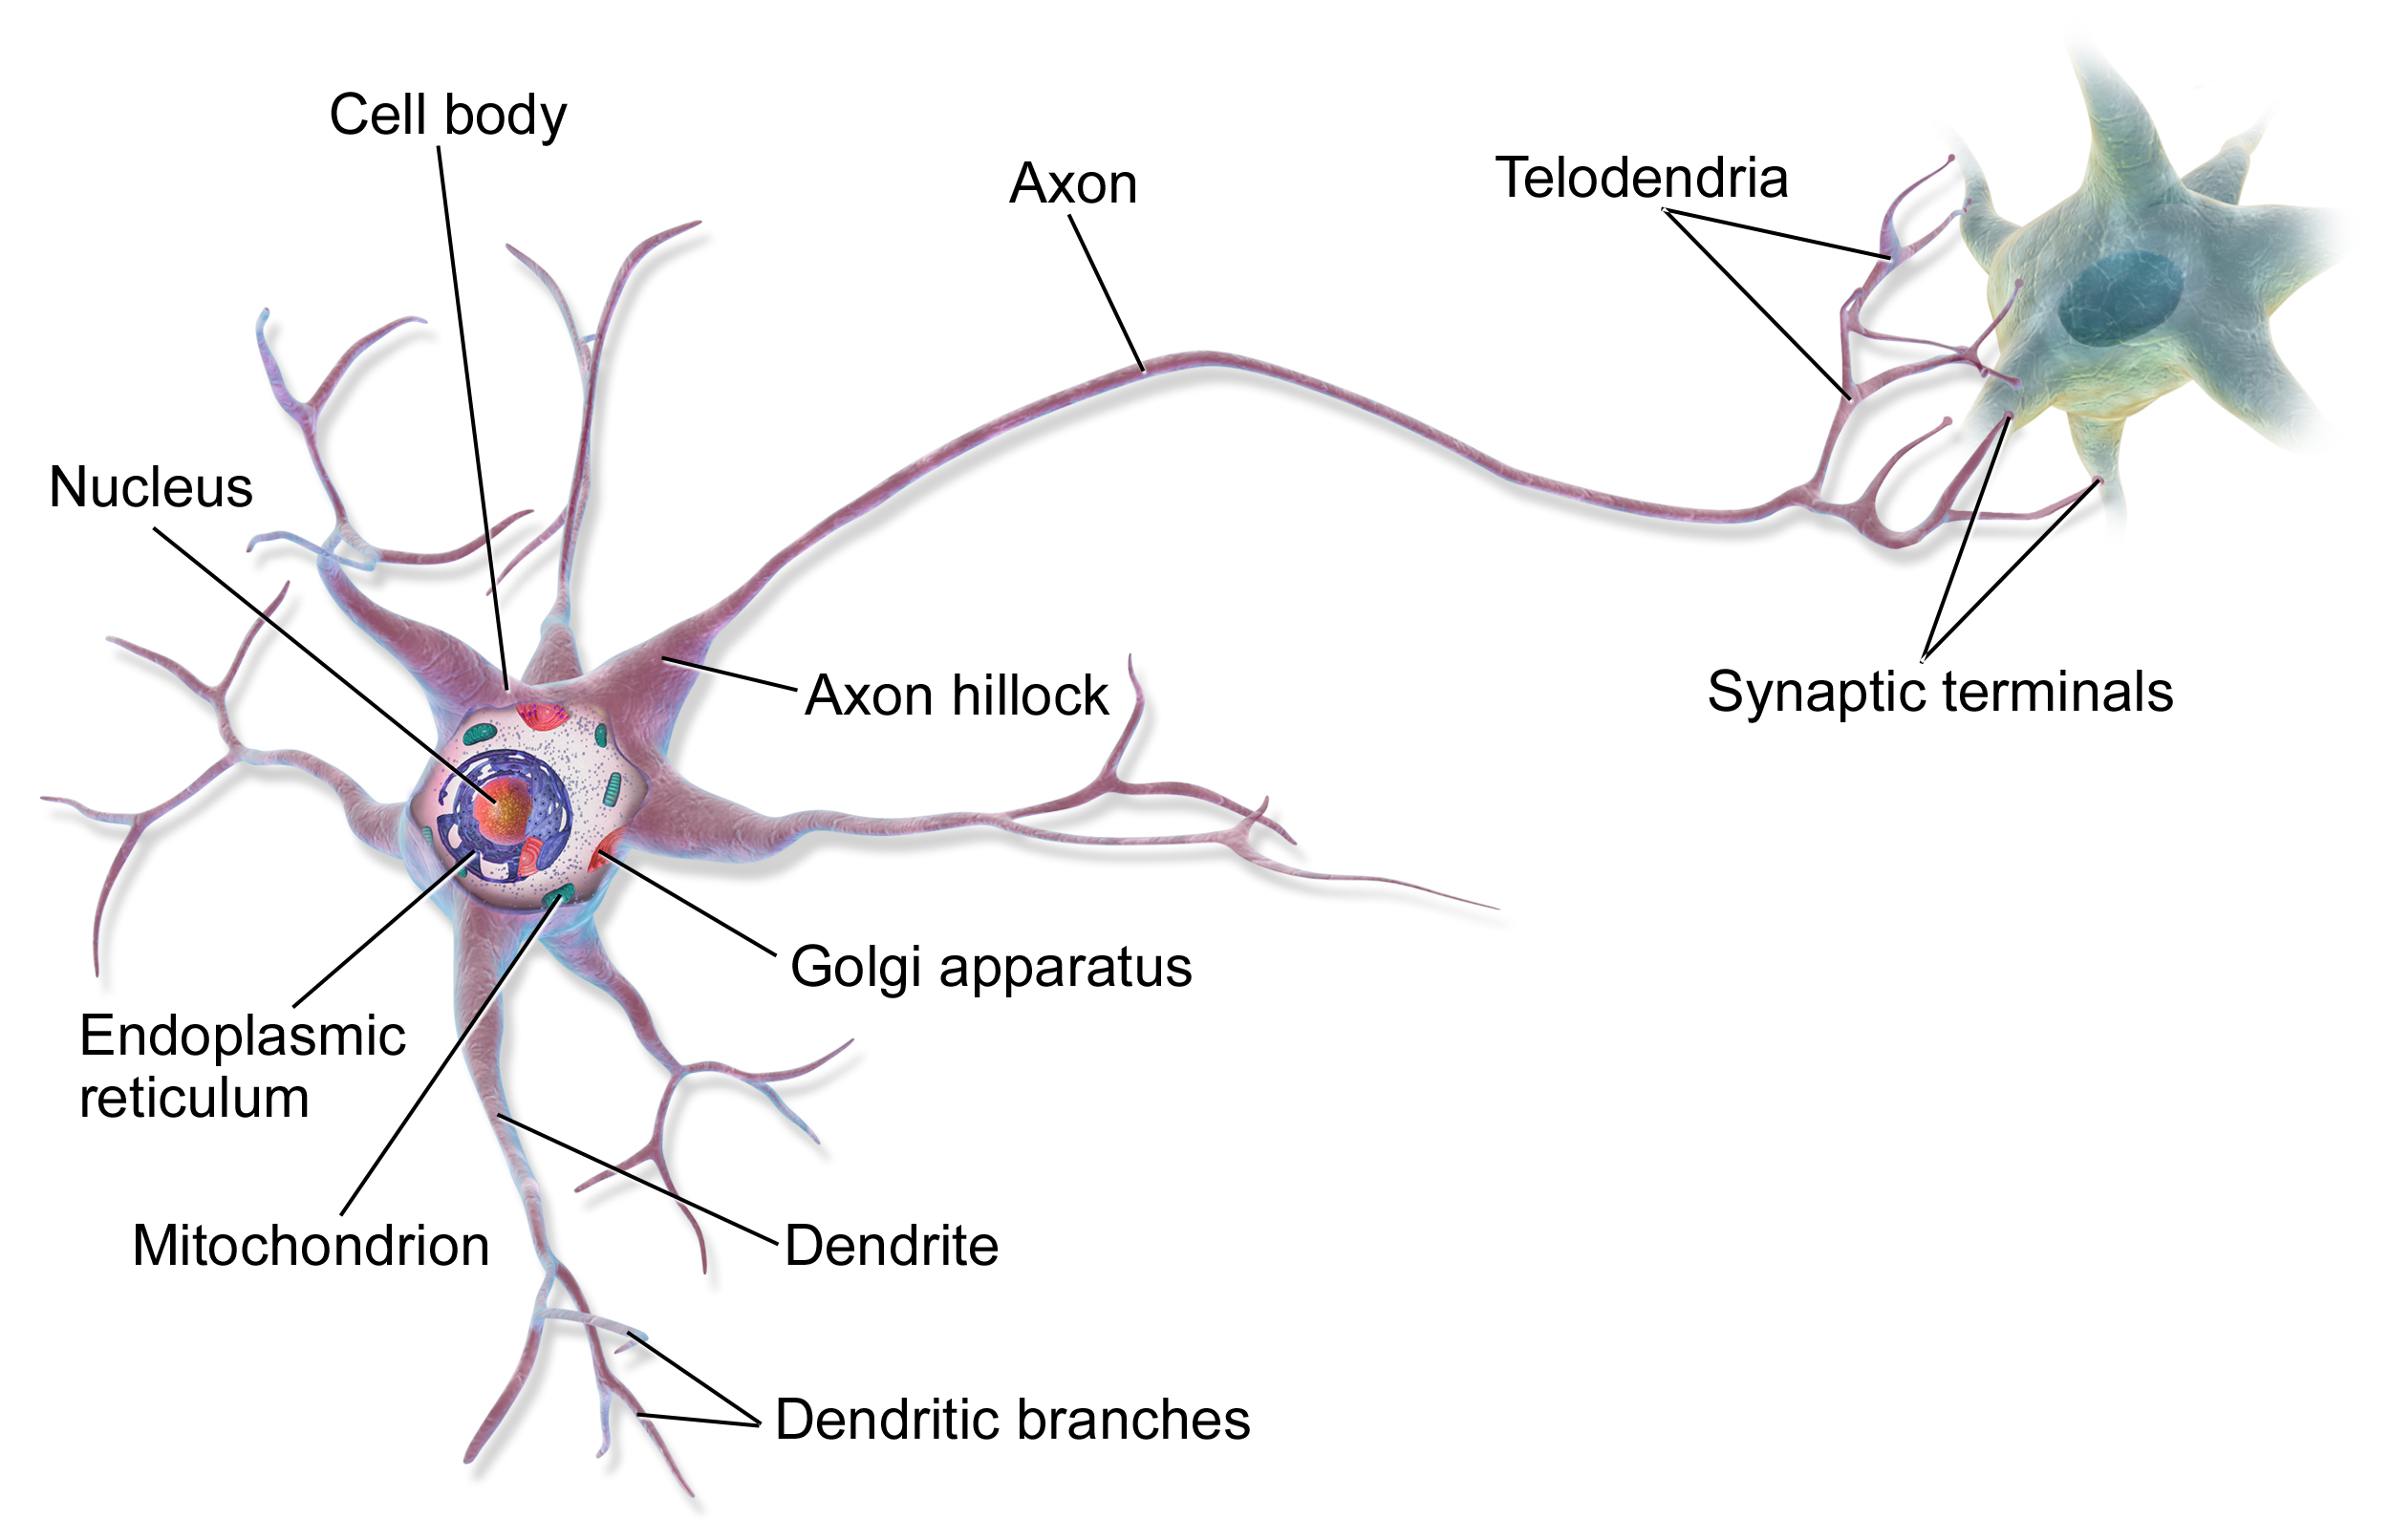
\includegraphics[width=0.5\textwidth]{images/neuron.png}
\end{figure}
The neuron is covered by the \textbf{neuronal membrane}, a phospholipid bilayer\footnote{A phospholipid bilayer is a two-layered arrangement of phosphate and lipid molecules that form a cell membrane. It serves as a continuous barrier around cells and organelles, separating the internal contents from the outside environment.}  which acts as a fatty barrier between the inside of the cell (cytoplasm) and the outside environment. This membrane is \textit{selectively permeable}: charged ions cannot pass through the bilayer, this allows the neuron to maintain different concentrations of chemicals on either side.

Since the membrane forms a barrier between the inside and the outside of the cell, the membrane uses specialized proteins to bridge the gap: The \textbf{Ion Channels} are ''tunnels'' that allow specific ions to flow in or out the membrane. By controlling the flow of positive and negative ions, the membrane creates an \textit{electrical difference} (voltage).\bigskip 

\noindent The main ion families that act in the neural cell are:\begin{itemize}
     \item Na$^+$: Sodium 
     \item K$^+$: Potassium 
     \item Cl$^-$: Chloride
     \item Ca$^{++}$: Calcium
\end{itemize}
The notation for the \textbf{valence} is the following, if an elements have $n$ $^+$ as supscript, it means that the atom is a positively charged ion that has lost $n$ electrons. Similarly, an element with $n$ $^-$ as supscript, is negatively charged, and had obtained $n$ electrons.
\begin{boxdefinition}{Ion Channels}{}
     An ion channel is a passive transportation channel where the ions can flow driven by electrochemical forces.
\end{boxdefinition}
\begin{figure}[H]
     \centering
     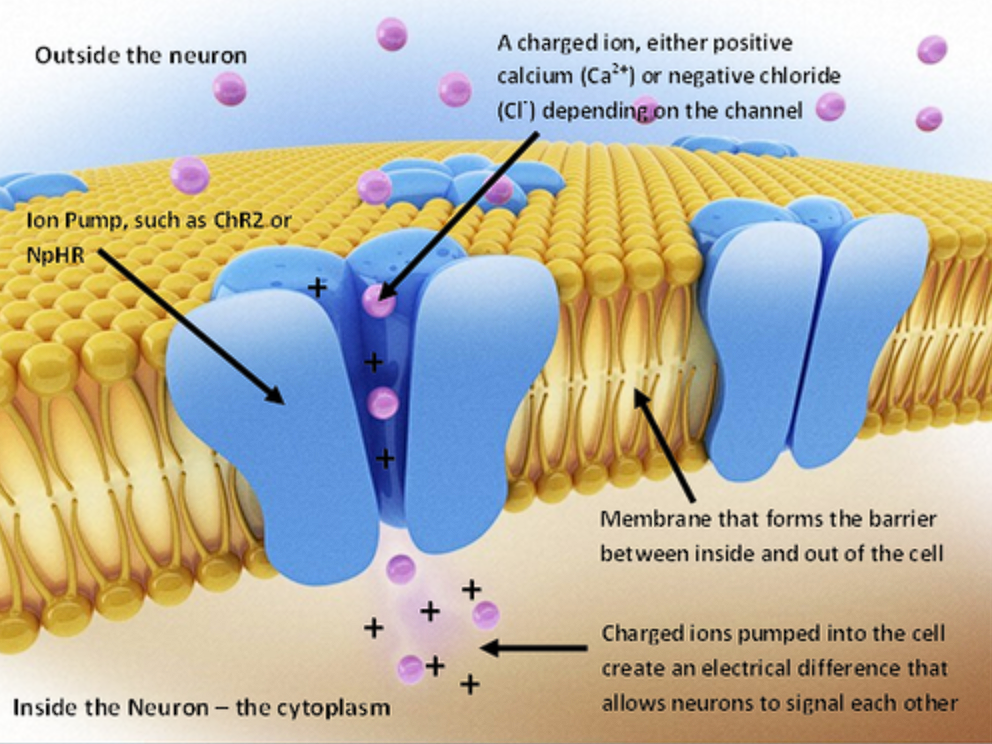
\includegraphics[width=0.5\textwidth]{images/neuralMembrane.png}
     \caption{A representation of the neural membrane.}
\end{figure}
An \textbf{Ion Pump} is an active transportation that requires an energy expenditure by
the cell, it allow ions to move into
and out of the cell by \textit{opening and
closing} in response to voltage
changes and to both internal and
external signals. 
\subsection{The Electrochemical Potential}
The movement of the ions in the neural cell is determined by two forces:\begin{itemize}
     \item \textbf{diffusional forces}: It is the natural tendency of substances to move from where they are highly concentrated to where they are less concentrated. We call this force the \textit{chemical gradient}. For example, if inside the cells the concentration of Potassium is 125 mM, and outside is 5mM, the diffusional force will push the Potassium K$^+$ outside.
     \item \textbf{electrical forces}: Since the ions are charged particles, they are attracted to the areas with opposite charge, we call this force the \textit{electrical gradient}. 
\end{itemize}
Each single ion will have an electrical gradient and a chemical gradient, equilibrium is reached when the (chemical) diffusion push is exactly equal and opposite to the electrical push. In this state, the net flux of that ion across the membrane is zero.
\begin{figure}[H] 
     \centering
     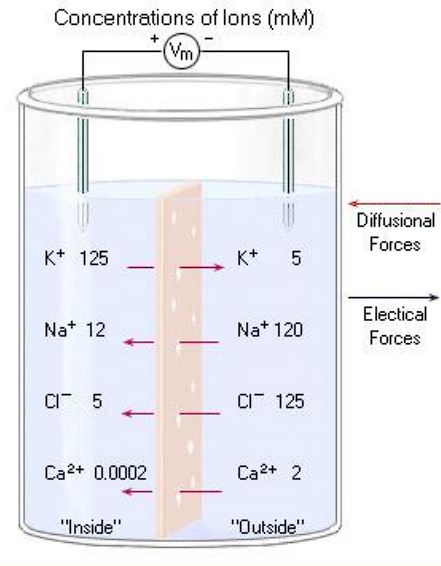
\includegraphics[width=0.3\textwidth]{images/membranePotential.png}
     \caption{A simple model of a neural cell.}
\end{figure}
\begin{boxdefinition}{Nernst Equation}{}
     The total gradient $\Delta\mu$ is given by the following equation:\begin{equation}
          \Delta\mu=RT\ln\frac{[X]_A}{[X]_B}+zF(E_A-E_B).
     \end{equation}
\end{boxdefinition}
$\Delta\mu$ is a scalar value that represents the difference in energy between the inside and the outside.\begin{itemize}
     \item $R$ is the universal gas constant.
     \item $T$ is the temperature in Kelvin. 
     \item $[X]_A$ is the ion concentration of the $A$ side of the membrane.
     \item $[X]_B$ is the ion concentration of the $A$ side of the membrane. Clearly $[X]_A$ and $[X]_B$  must share the same unit of measurement (usually mM).
     \item $z$ is the ion valence (e.g: +2 for Ca$^{++}$; -1 for Cl$^-$).
     \item $E_A-E_B$ is the energy resulting from the electric potential difference between the two sides.
\end{itemize}
Note how we are generally talking about a side $A$ and a side $B$, to distinguish between the outside and the inside of a membrane. There is an \textbf{electrochemical equilibrium} when $\Delta\mu=0$. For each family of ions $j$, we can compute the electrochemical equilibrium potential:\begin{align}
     &RT\ln\frac{[X]_A}{[X]_B}+zF(E_A-E_B)=0\implies\\
     &-zF(E_A-E_B)=RT\ln\frac{[X]_A}{[X]_B}\implies\\
     &E_j=E_A-E_B=-\frac{RT}{zF}\ln\frac{[X]_A}{[X]_B}.
\end{align}
$E_j$ is usually measured in mV and represents the exact electrical voltage value needed to stop the net movement of a specific ion across the membrane. Is the voltage at which the diffusional forces balance the electrical ones for the $j$ ions. Typical values are:\begin{itemize}
     \item Potassium: $E_{\text{K}^+}=-90$mV.
     \item Sodium: $E_{\text{Na}^+}=50$mV.
     \item Calcium: $E_{\text{Ca}^{++}}=-150$mV.
\end{itemize}
Remember that, despite the gradients, an ions is not always free to cross the membrane. For a given ion family with electrochemical equilibrium potential $E_j$, if the current potential is $E_j+\epsilon$ with $\epsilon\in \R$, in the moment that the ions are free to cross the
membrane, they will flow with net currents that move the membrane
potential to that value.\begin{enumerate}
     \item The cell is at $-70 $mV, but the Sodium (Na$^+$) would like to be at $+60 $mV ($E_j$). As long as the channels are closed, Sodium is blocked.
     \item Opening of the sodium channels: Since the current potential ($-70$) is not the equilibrium potential ($+60$), there is a huge push. Sodium ions begin to enter the cell en masse.
     \item This flow of positive charges (current) changes the membrane voltage, ''dragging'' it from $-70$ towards $+60$.
\end{enumerate}
\begin{boxdefinition}{Ion Pumps}{}
     The ion pumps are specialized proteins inside the membrane that actively push the ions against their gradient, to have a rest potential different than zero, an active transporter for the ions is needed, if not, the ions would move towards the gradient direction so as to set to zero the gradient.
\end{boxdefinition}

This is why at ''rest'', the potential is not zero. These ion pumps are constantly working and transforming ATP\footnote{
     ATP (adenosine triphosphate) is the main energy exchange molecule of the cell, acting as a sort of universal ''energy currency''.
} to push the ions.
\begin{quote}
    The resting potential (about -70 mV) is the result of a delicate balance: the membrane passively lets out some potassium, while the sodium-potassium pump constantly works as a ''maintenance machine'' to put the ions back where they belong, keeping the inside of the cell negative compared to the outside.
\end{quote}
\begin{figure}[H] 
     \centering
     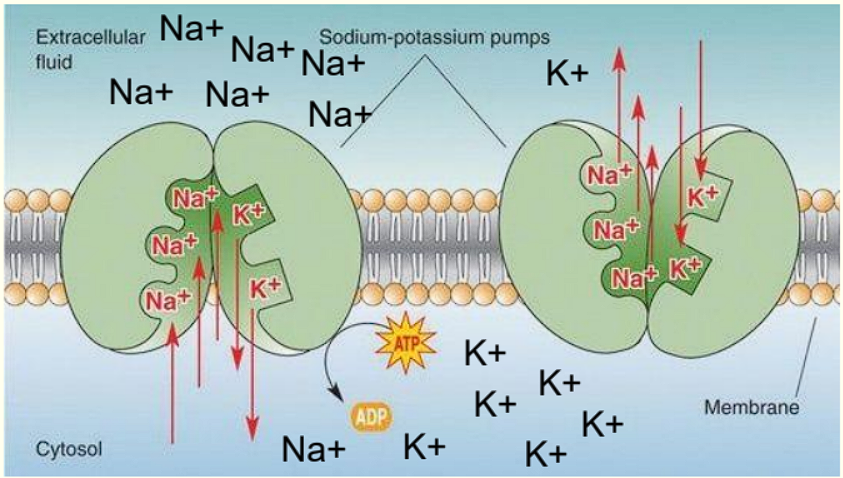
\includegraphics[width=0.5\textwidth]{images/ionPumps.png}
     \caption{The sodium-potassium pumps.}
\end{figure}
We already explained that any single family of ions have a electrochemical equilibrium potential (the potential needed to counter back the diffusional forces). 
\begin{boxdefinition}{Membrane Potential}{}
     The \textbf{membrane potential} is the \textit{difference in electrical potential} between the interior of a neuron and the surrounding extracellular fluid, given by the different ion concentration on the two ends of the membrane. At rest, this potential is around $-70$mV, so it's \textit{polarized}.
\end{boxdefinition}
The membrane potential is the weighted average of the equilibrium potentials of all the ions present, based on the permeability of the membrane to each of them.
\begin{figure}[H] 
     \centering
     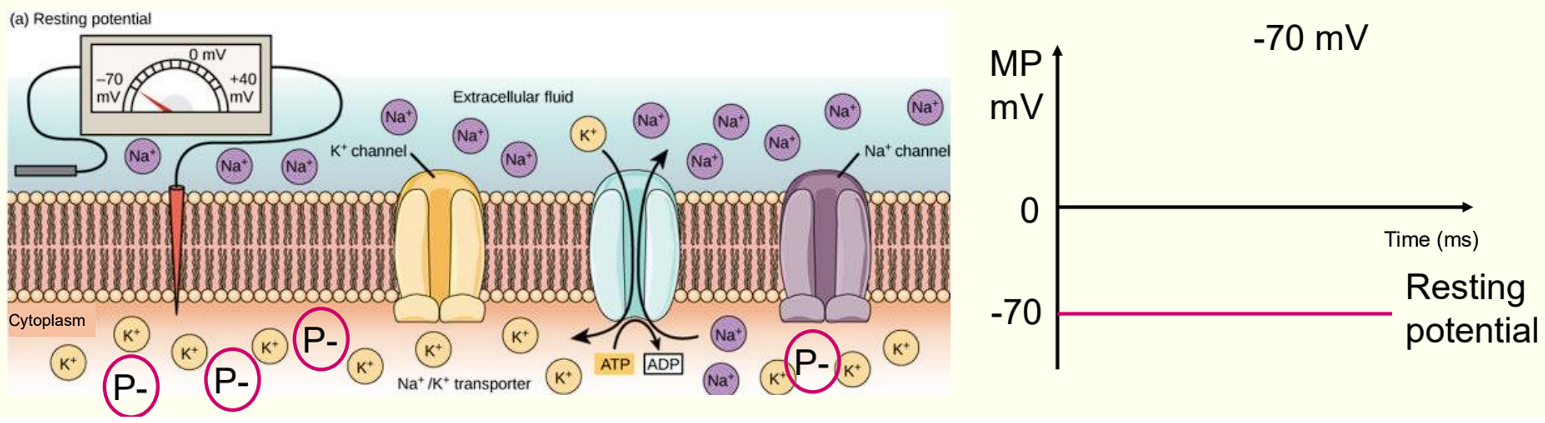
\includegraphics[width=\textwidth]{images/membranePotential2.png}
     \caption{Membrane potential.}
\end{figure}
When a current of positively charged ions flows into the cell, or a current of negatively charged ions flows out, the membrane potential arise becoming less negative or even positive, this phenomena is called \textbf{depolarization}. Similarly, if a current of positively charged ions flows out, or a current of negatively charged ions flows into the cell, there is a \textbf{repolarization}, or an \textbf{hyperpolarization} if the potential goes below the rest $-70$mV.
\begin{figure}[H] 
     \centering
     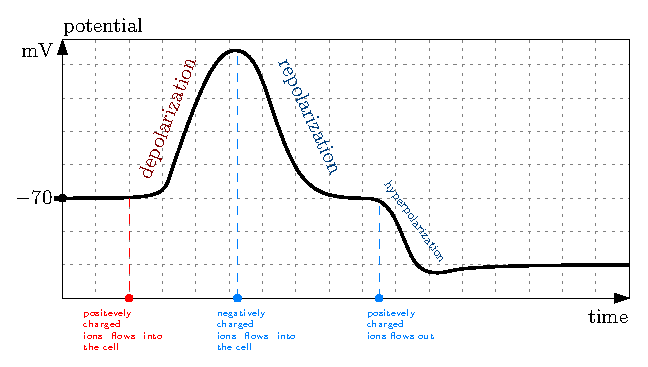
\includegraphics[width=0.8\textwidth]{images/polarization.eps}
\end{figure}
\section{Communication Between the Neurons}
\subsection{Synapses}
The neuron is structured as a ramified structure called \textbf{dendritic tree}, the branches called dendrite have the task to collect and propagate information from the other neural cells. A \textbf{synapses} is the structure that allows the communication between different neurons, a single neuron receives thousands of input (synapses) signals.

To a neuron, might arrive a burst of signals from the same synapses near in time, or different signals coming from different synapses, in this way the neuron receives a signal that is a \textit{summation} in time and space.\bigskip

In an exchange of information, the neuron that send the signal is called \textit{presynaptic neuron}, the one that receives is the \textit{postsynaptic neuron}. 
There are two types of synapses:\begin{itemize}
     \item \textbf{Electrical synapses}: The ions pass directly from the presynaptic to the postsynaptic cell. Is the fastest type of communication and is almost instantaneous.
     \item \textbf{Chemical synapses}: The chemical signals are mediated by the \textit{neurotransmitters} that cause the opening of specific ion gates channels, making the ions pass from a neuron to the other, pushed by the gradient.
\end{itemize}



\begin{figure}[H] 
     \centering
     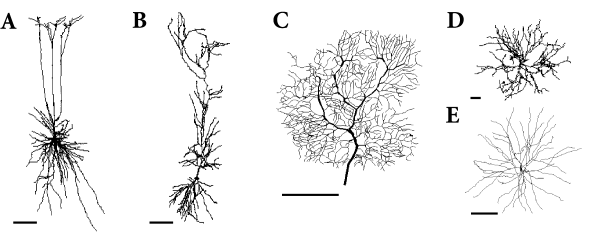
\includegraphics[width=0.6\textwidth]{images/tree.png}
     \caption{Different kinds of dendritic tree configurations.}
\end{figure}


The two membranes of different neurons that have to communicate aren't in contact, there is a \textit{Gap Junction}. This gap is around $3.5$nm for the electrical synapses and $20-40$nm for the chemical synapses.


\begin{figure}[H] 
     \centering
     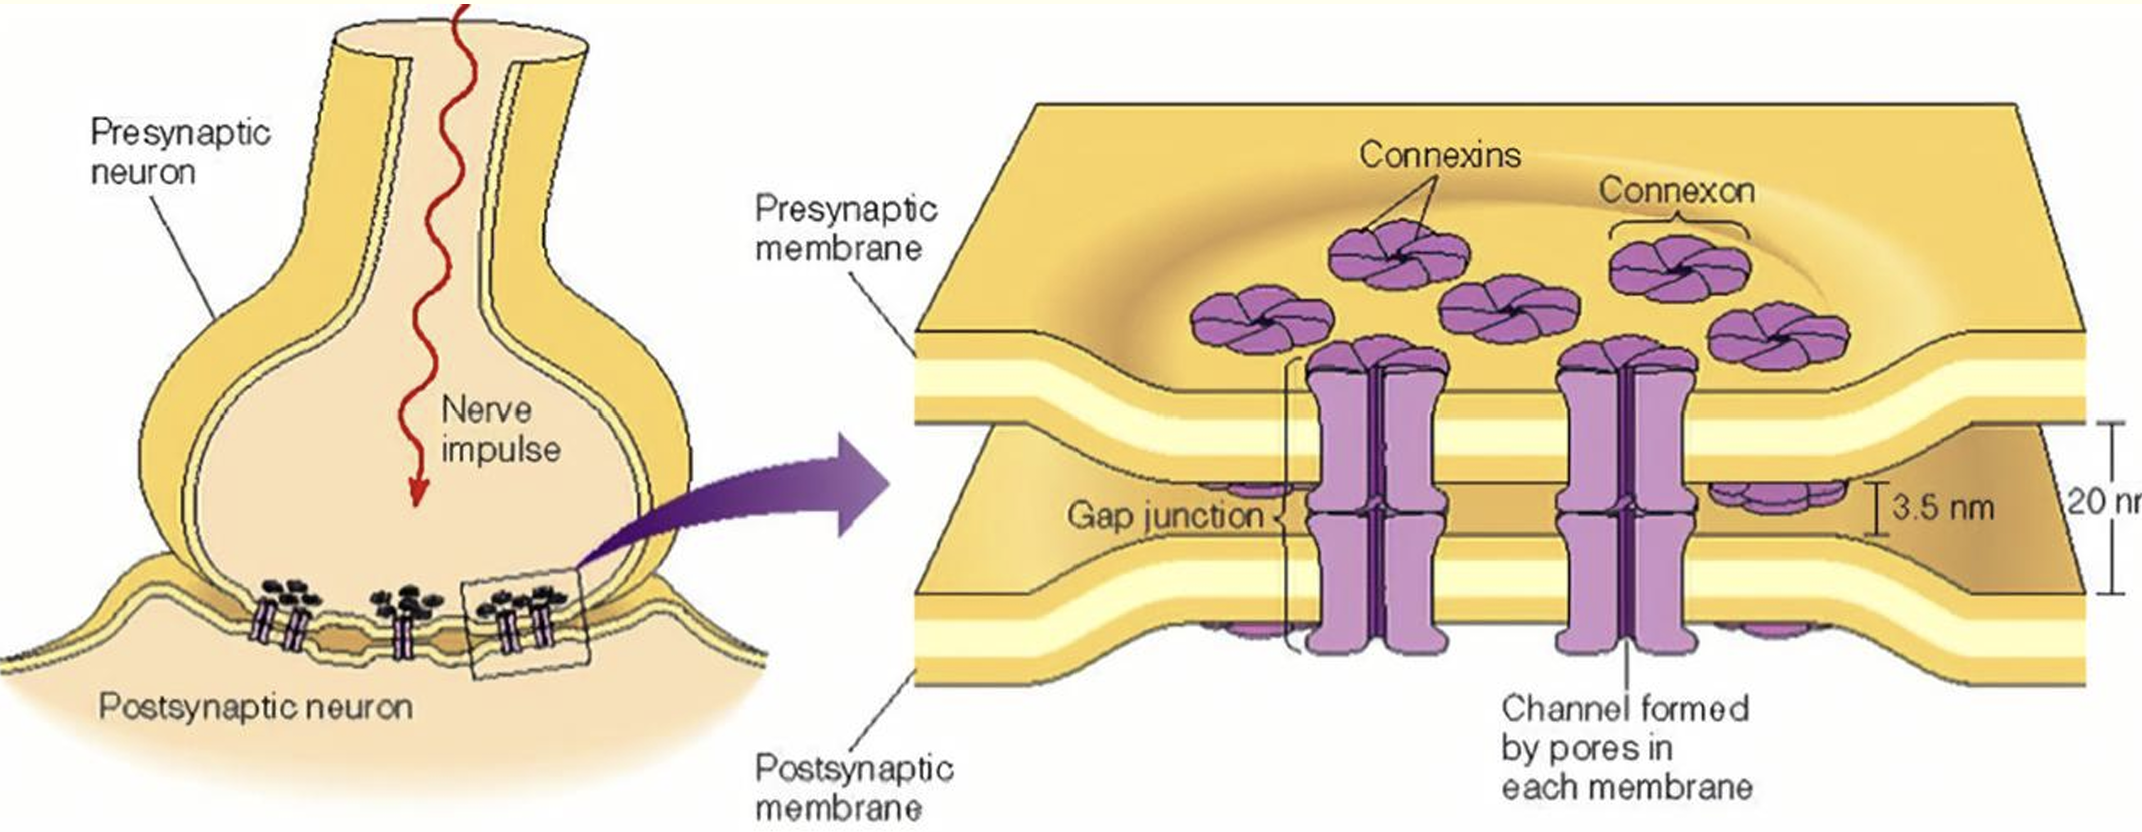
\includegraphics[width=0.6\textwidth]{images/neuronCommunication.png}
     \caption{Electrical synapses.}
\end{figure}

After a synapses, some ions pass from a neural cell to an other, causing these two to change their potential.\begin{itemize}
     \item \textbf{Excitatory synapses}: When some ions pass to the postsynaptic cell by depolarizing the potential.
     \item \textbf{Inhibitory synapses}: The opposite case, when the communication cause an hyperpolarization of the postsynaptic neuron potential.
\end{itemize}
\begin{figure}[H] 
     \centering
     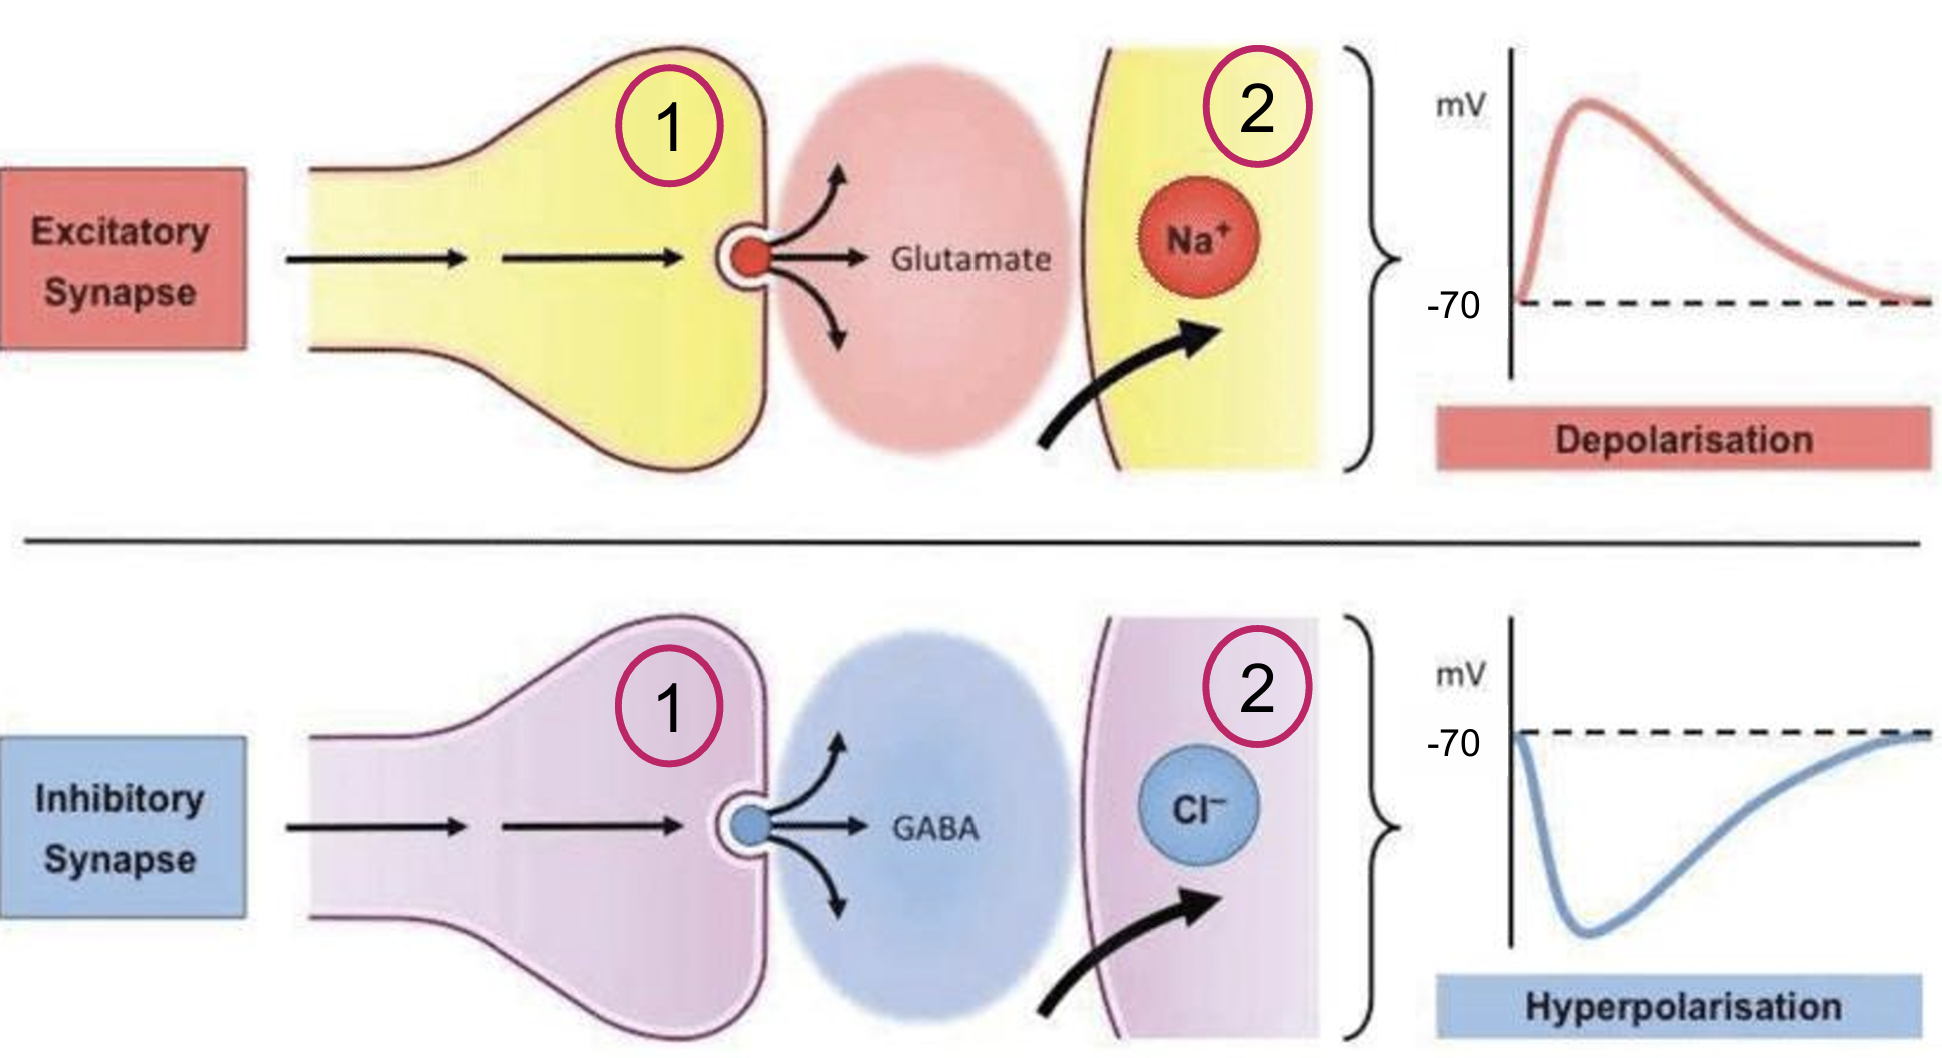
\includegraphics[width=0.5\textwidth]{images/exc_and_inh.png}
\end{figure}
\subsection{Action Potential}
When a single neuron release neurotransmitters, generates a potential that depolarize the membrane, but is not enough to create an \textit{action potential}, the signal returns back to the rest condition at $-70$ mV.  
If more presynaptic neurons fires a signal through different points of the dendrite to the same postsynaptic neuron, there is a \textbf{spatial summation effect}, these small potentials sum, generating a much higher potential.
If a single presynaptic neuron fires a burst of potential near in time, there is a \textbf{temporal summation effect}, since the ion channels have not yet closed completely from the first stimulus, the second EPSP is added to the ''tail'' of the previous one.
\begin{figure}[H] 
     \centering
     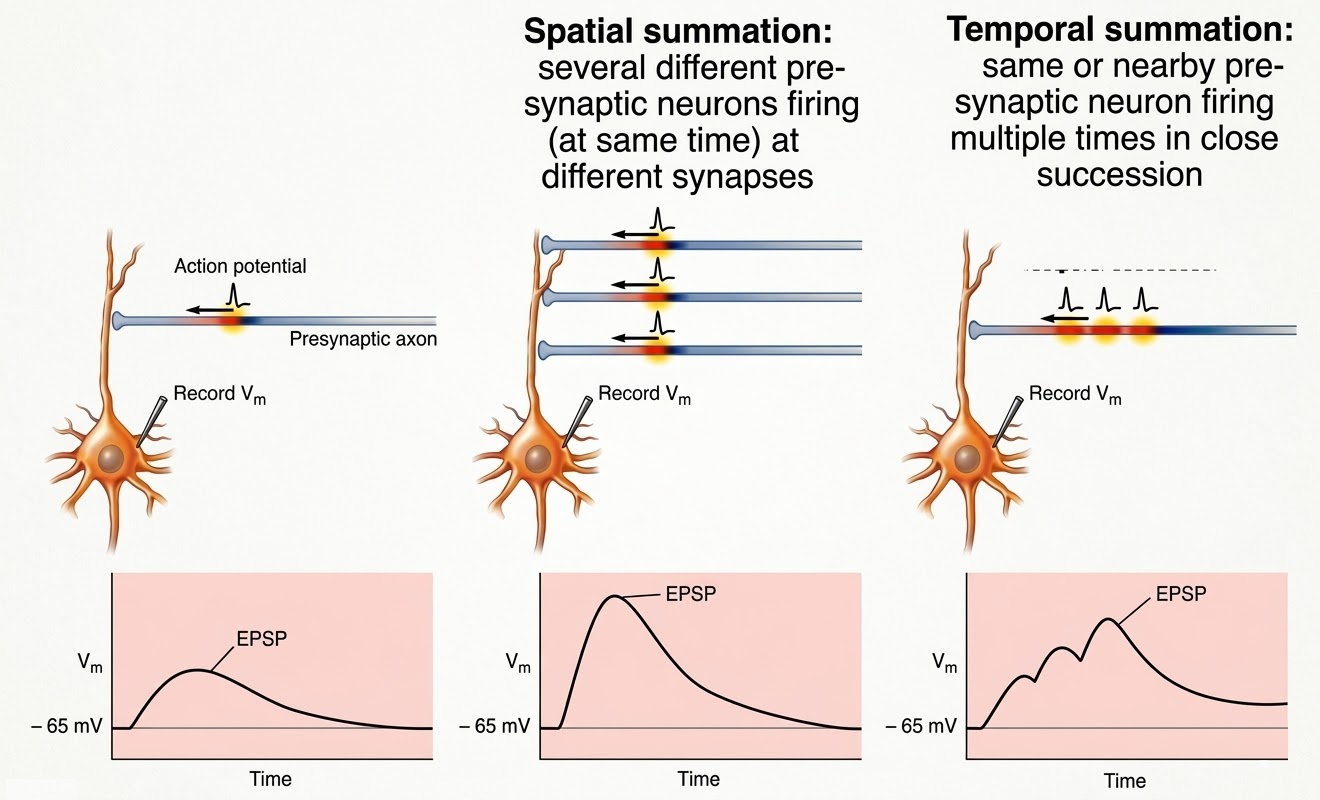
\includegraphics[width=0.7\textwidth]{images/summation_synapses.png}
\end{figure}
The presynaptic signals sent to a neuron are binary, these action potentials are spikes, that can be inhibitory or excitatory, all these signals are summed in the postsynaptic neuron creates a potential that changes continuously over time.
\begin{figure}[H] 
     \centering
     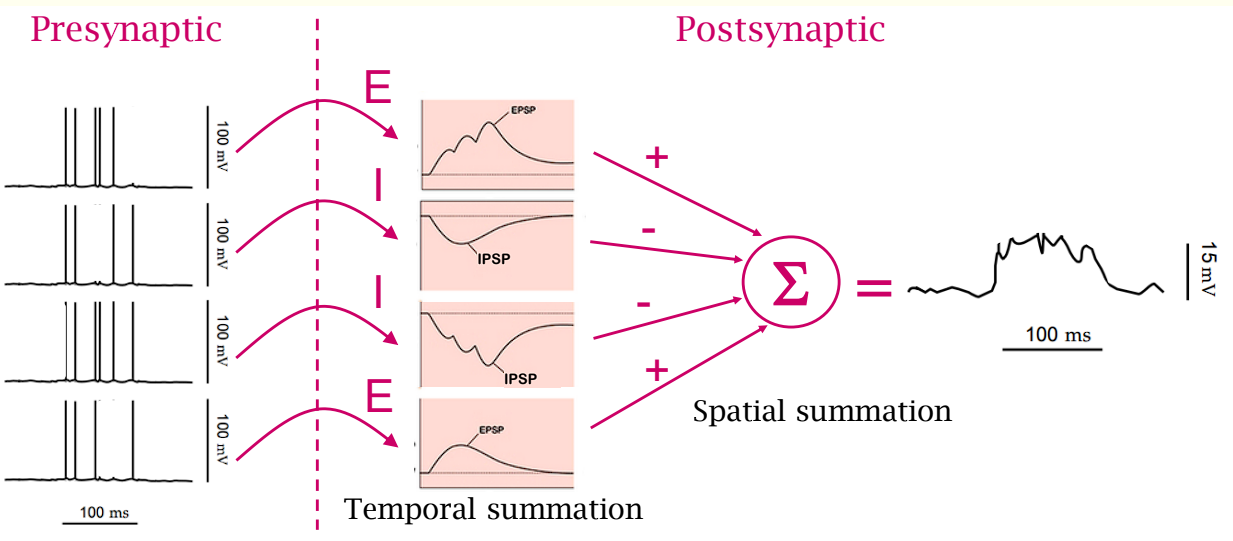
\includegraphics[width=0.7\textwidth]{images/summation_synapses2.png}
\end{figure}
So, the information processed by the neurons is composed by the sum of these excitatory and inhibitory post synaptic signals, the spatial and temporal summation produce the membrane polarization/depolarization, and this result is propagated along the membrane up the axon hillock (the physical point where all the EPSPs and IPSPs collected by the dendrites and soma converge. Here the algebraic sum of the signals takes place). According to the result of this summation, the cell may or not may fire an \textit{action potential}.
\begin{boxdefinition}{Action Potential}{}
     The action potential (or spike) is a rapid, temporary, self-reflexive reversal of a neuron's resting membrane potential.
\end{boxdefinition}
The potential abruptly goes from about $-70\text{ mV}$ (rest) to about $+30$ or $+40\text{ mV}$, and then rapidly returns to the negative state. This process occurs in approximately 1-2 milliseconds.
If the sum of EPSPs at the axon hillock exceeds the threshold (about $-55\text{ mV}$), the voltage-gated sodium ($Na^+$) channels open wide. Sodium enters massively into the cell, making it positive.\bigskip

It's a \textit{all or none} process, if the stimulus does not reach the given threshold, nothing happens, else, the spike have always the same shape, duration and intensity, it's a \textbf{binary decision}.\begin{itemize}
     \item \textbf{The Sodium Channel}:\begin{enumerate}
          \item At the resting potential $-70\text{ mV}$, the gate is closed, the ions Na$^+$ can't pass. 
          \item When the membrane depolarize and reach the threshold (about $-55\text{ mV}$), the sodium gates open, and the ions pass quickly in the gates following the electrochemical gradient, producing a raise in the action potential. 
          \item At the peak of this spike, an \textit{inactivation port} activates, closing the gates from the inside, the channel is closed and can't be re-opened immediately. This is called \textbf{absolute refractory period}: No
new action potential can be
produced (under any
circumstances).
     \end{enumerate}
     \item  \textbf{The Potassium Channel}:\begin{enumerate}
          \item It is closed during rest and during the first rising phase of the spike.
          \item It opens with a certain delay compared to that of sodium, typically when the spike has reached it's peak.
          \item When it opens, the potassium K$^+$ leaves the cell (because it is less concentrated outside). This release of positive charges causes the membrane potential to collapse, bringing it back down (repolarization).
          \item Because it closes slowly, too much potassium often escapes, bringing the membrane to a more negative value than rest (e.g. -80 mV), causing post-potential hyperpolarization (undershoot).
     \end{enumerate}
\end{itemize}
\begin{figure}[H] 
     \centering
     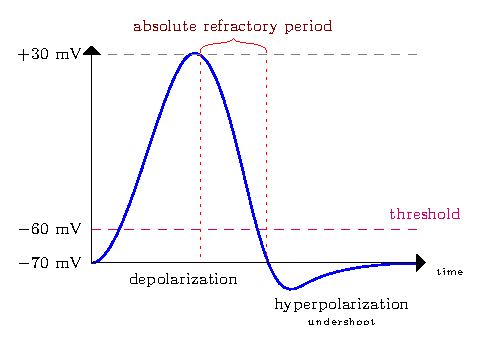
\includegraphics[width=0.6\textwidth]{images/spike.eps}
\end{figure}
All the spikes have the same shape, the same duration (2 milliseconds) and the same amplitude (100 mV), are fast and intense. Once the action potential is generated in the axon hillock, it needs to be propagated along the axon towards other cells. There are two main mechanisms.\bigskip 

In \textbf{Continuous Conduction}, the action potential is continuously generated at each membrane section , the fast membrane depolarization induces an intra and extra cellular ionic currents, that propagate the perturbation to close membrane regions. If it finds Na$^+$ channels ready to open, the depolarizing perturbation produces
again an action potential (active generation).
\bigskip

If the close membrane region has just produced an action potential, the Na$^+$ channels will be in their absolute refractory period, if so, a new action potential will be impossible to produce. The propagation speed is around 1 meter per second.

The absolute refractory causes the \textbf{unidirectional} of the action potential propagation:  As the action potential propagates forward towards the ''closed'' (ready to fire) channels, the membrane segment just passed through is in the refractory period. Even if the electric charges (local currents) try to diffuse backwards, they find inactivated Na$^+$ channels that do not respond. 

\begin{figure}[H]
     \centering
     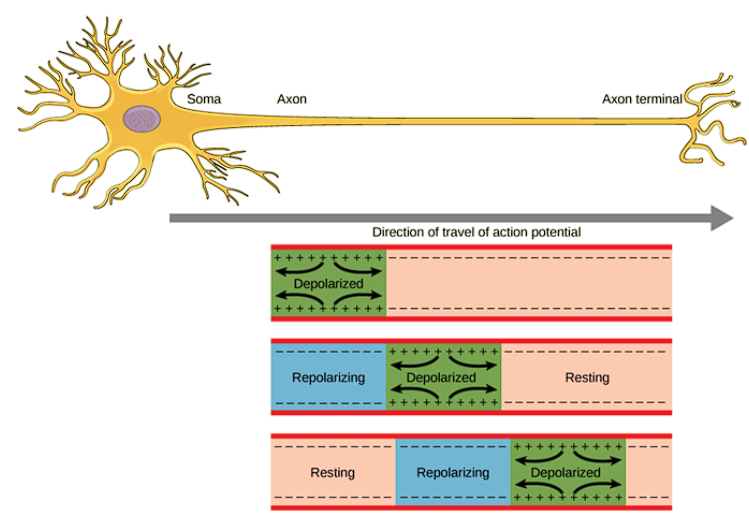
\includegraphics[width=0.5\textwidth]{images/ContinuousConduction.png}
     \caption{Continuous Conduction.}
\end{figure}

\textbf{Saltatory Conduction} is the mechanism by which an action potential propagates along a myelinated axon. Instead of flowing continuously across the entire membrane, the pulse ''jumps'' from one non-isolated point to another.\bigskip

In axons, the membrane is surrounded by an insulating sheath called myelin (formed by Schwann cells in the PNS and oligodendrocytes in the CNS).

The myelin sheath functions as an electrical insulator which dramatically increases the membrane's resistance ($R_m$) and reduces it's capacitance ($C_m$).
The \textit{nodes of Ranvier} are short breaks in the sheath (about 1-2 $\mu$m) where the axon membrane is exposed to extracellular fluid. Only here is a very high density of voltage-gated sodium (Na$^+$) channels found.\bigskip 

When a spike is generated in a node of Ranvier, sodium ions enter the cell. Because myelin prevents charges from ''leaking'' across the membrane (high $R_m$), electric current flows almost instantaneously within the axon to the next node.
The speed is much higher than that of sequential opening of channels.
Before the electrical signal fades too much, it reaches the next Ranvier node. Here, the depolarization is still sufficient to exceed the threshold, triggering the opening of local Na$^+$ channels.

\begin{figure}[H]
     \centering
     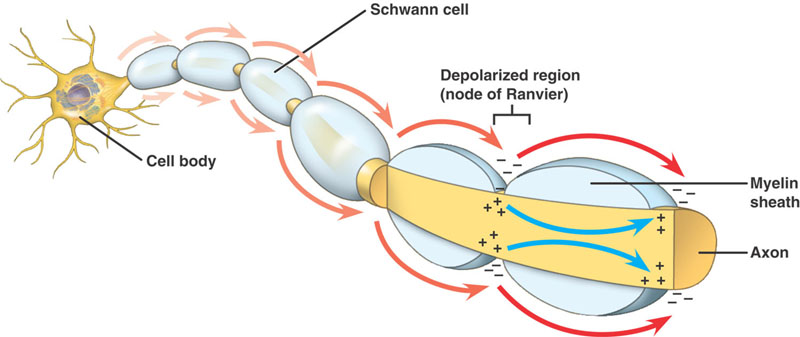
\includegraphics[width=0.6\textwidth]{images/SaltatoryConduction.jpg}
     \caption{Saltatory Conduction.}
\end{figure}

\chapter{Principles of Neuroanatomy}
The brain processes incoming information to guide decisions by integrating sensory inputs with encoded and retrieved past experiences.\bigskip

Scientific study of the brain dates back centuries, with evidence of Ancient Egyptian trepanation. Historically, cerebral architecture was mapped primarily through \textbf{lesions} analysis, identifying functional specialization by observing the specific impairments caused by brain damage. \bigskip


Modern neuroscience employs a variety of approaches to study neural activity:
\begin{itemize}
    \item \textbf{Invasive Procedures:} Historically, animal studies allowed for invasive techniques that are ethically and practically unfeasible for human subjects. These studies provided the groundwork for understanding cellular-level interactions.
    \item \textbf{Neuroimaging Techniques:} In recent decades, non-invasive methods have revolutionized the field. A prominent example is the \textbf{EEG (Electroencephalography)}, which measures fluctuations in the electrical fields perturbed by neuronal activity.
\end{itemize}
Modern technology enables active brain modulation using external electrical or magnetic fields to temporarily interfere with neural circuits. These ''reversible lesions'' allow researchers to study behavioral contributions of specific areas without permanent damage. \bigskip

The brain's primary role is processing information for decision-making, a cycle based on receiving, encoding, and retrieving data from past experiences. While interest in the brain dates back to Ancient Egyptian neurosurgery, for centuries our understanding of cerebral architecture relied on observing clinical \textbf{lesions} to map functional specialization through compromised abilities.

\bigskip

In neuroengineering, no single spatial or temporal scale suffices for a complete brain study. The brain functions across a vast spectrum; while neural activity is generally measured in milliseconds, the kinetics of ion channel gates—specifically their opening and closing—occur in fractions of a millisecond. This sub-millisecond range defines the highest resolution necessary for sophisticated neural analysis. \bigskip

Spatially, investigation reaches the micrometer ($\mu m$) level, essential for analyzing the soma or the nanometer-scale ($nm$) neuronal membrane. While global brain analysis rarely requires such granularity, it is vital for understanding cellular neurobiology. Moreover, the brain is dynamic, evolving through species-wide and individual neuroplasticity. This lifelong characteristic enables learning, memory, spontaneous recovery, and neurorehabilitation. \bigskip

Modern research employs both invasive (mostly animal-based) and non-invasive methods, such as Electroencephalography (EEG), to study electrical field perturbations from neuronal firing. Beyond observation, researchers can actively modulate brain activity using external electrical fields to simulate ''reversible lesions.'' This allows for the real-time study of how specific circuits contribute to behavior without causing permanent impairment.

\section{Brain Organization}
The brain's anatomical composition is divided into \textbf{grey matter} (cell bodies and dendrites) and \textbf{white matter} (myelinated axons), characterized by a high lipid content. These tissues are visualized \textit{in vivo} using MRI, while \textbf{Diffusion Tensor Imaging (DTI)} specifically enables white matter tractography to map neural fiber trajectories.

\begin{figure}[H] 
     \centering
     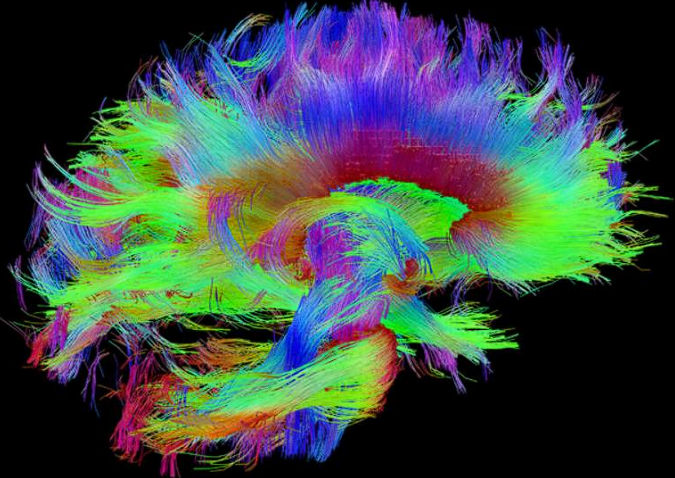
\includegraphics[width=0.5\textwidth]{images/DTIimage.png}
     \caption{DTI scan.}
     \label{DTI}
\end{figure}
The \textbf{corpus callosum} is the primary white matter tract ensuring inter-hemispheric connectivity; its degradation is a key clinical indicator of neural network breakdown. \bigskip

The \textbf{cerebral cortex} maximizes its surface area within the skull through a folded architecture of \textbf{gyri} and \textbf{sulci}, with the latter accounting for two-thirds of the total area. Despite representing only 1.5\% of body weight, the cortex's high-level processing requires 15\% of total blood flow, underscoring its significant metabolic demands. \bigskip
\begin{figure}[H] 
     \centering
     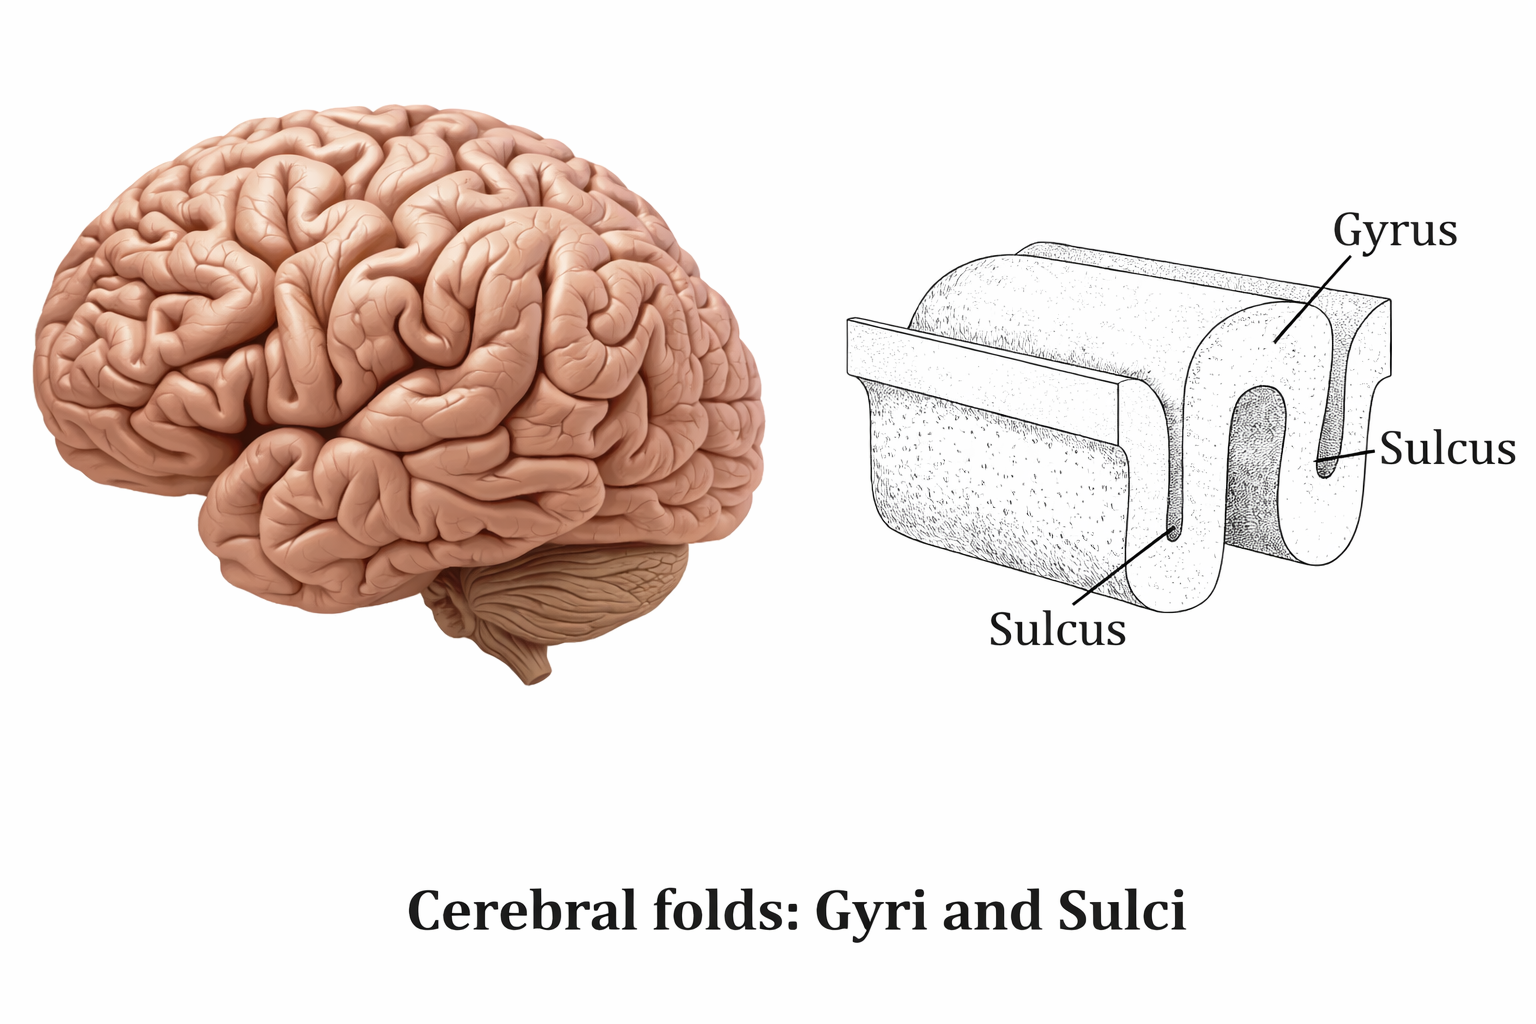
\includegraphics[width=0.7\textwidth]{images/gyry_sulci.png}
\end{figure}
The internal cortical architecture follows a modular organization of \textbf{six vertical layers} and \textbf{cortical columns} ($\approx$ 0.5 mm diameter). These layers facilitate the outward spread of information, while the columns serve as the basic functional unit. Neurons within a single column exhibit identical responses to specific stimuli, collaborating on a computational task while adjacent columns process different aspects of that function.
\begin{figure}[H] 
     \centering
     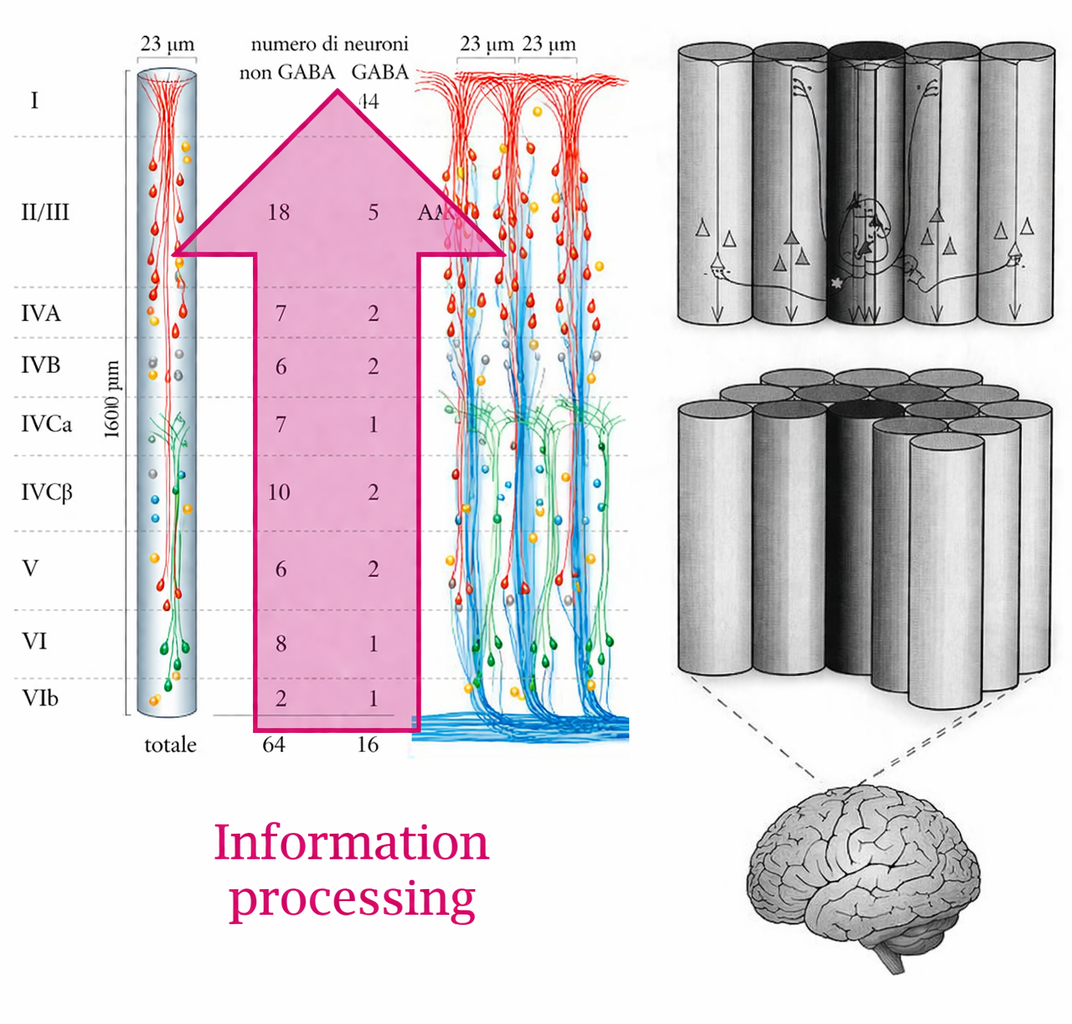
\includegraphics[width=0.5\textwidth]{images/cortical_columns.png}
\end{figure}
Neural communication is facilitated by three primary connection types, which can be either \textbf{excitatory} or \textbf{inhibitory}. \textbf{Feedforward (bottom-up)} connections transmit signals to subsequent processing stages, while \textbf{feedback (top-down)} connections relay information back to earlier regions. The majority of neural circuitry consists of \textbf{lateral} connections, which link regions at the same processing level, essential for local integration and modulating neighboring functional units.
\begin{figure}[H] 
     \centering
     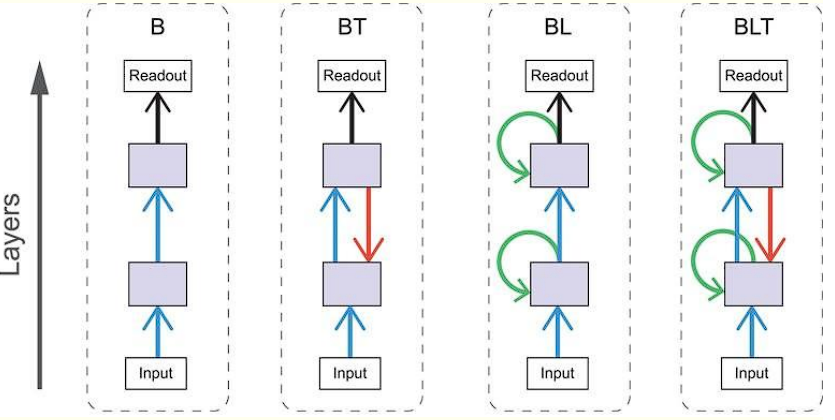
\includegraphics[width=0.5\textwidth]{images/bottom_up.png}
\end{figure}
\section{Functional Mapping and Specialization}
\begin{figure}[H]
  \centering
  \begin{minipage}{0.4\textwidth}
    \centering
    \includegraphics[width=\textwidth]{images/zonecervello.png}
  \end{minipage}
  \hfill
  \begin{minipage}{0.5\textwidth}
    To navigate brain topography, standardized anatomical axes are utilized for precise regional identification. Primary longitudinal descriptors include \textbf{Anterior/Posterior} (front/behind), \textbf{Superior/Inferior} (above/below), and \textbf{Rostral/Caudal} (nose/tail). Spatial orientation relative to the midline is defined by \textbf{Medial/Lateral} axes, while lateralized functions are termed \textbf{Ipsilateral} (same side) or \textbf{Contralateral} (opposite side). Finally, the \textbf{Dorsal/Ventral} axis distinguishes between the ''back'' and ''belly'' aspects, accounting for the neuroaxis curvature relative to the spinal cord.
  \end{minipage}
\end{figure}
At a macro-anatomical level, the brain is divided into four lobes named after their protecting cranial bones. While structurally symmetrical, functional asymmetries exist, such as language processing in the \textbf{frontal lobe}, which governs executive functions like reasoning and motor planning. \bigskip

The other lobes specialize in distinct domains: the \textbf{parietal lobe} integrates somatosensory data and spatial orientation; the \textbf{occipital lobe} interprets visual stimuli; and the \textbf{temporal lobe} processes auditory information and receptive language. The latter also houses the \textbf{hippocampus}, vital for memory, emotion, and spatial mapping. This lobar division serves as a functional map of a highly interconnected system. \bigskip
\begin{figure}[H] 
     \centering
     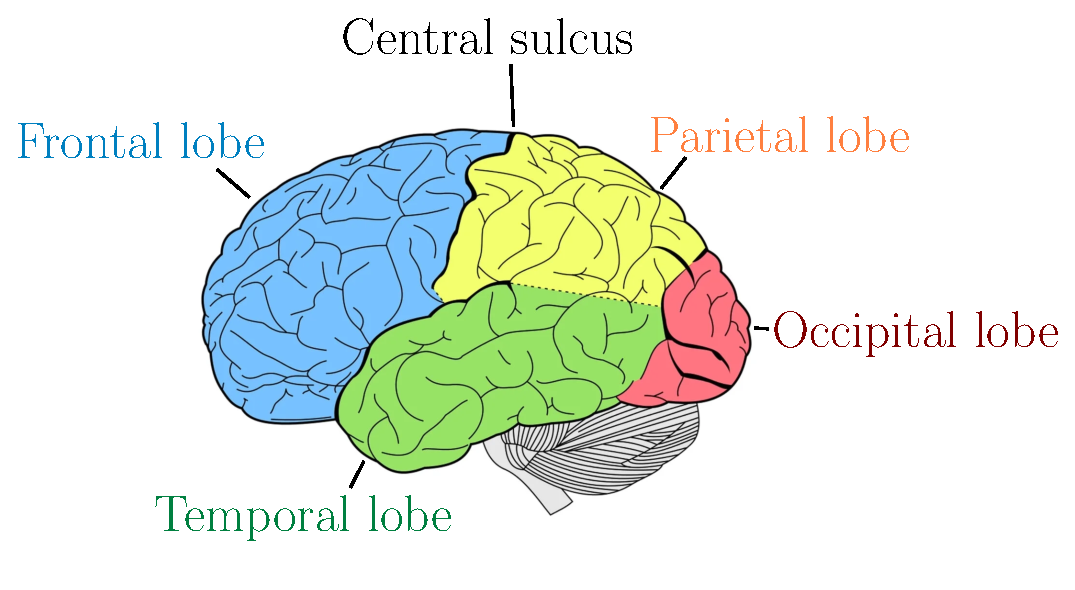
\includegraphics[width=0.6\textwidth]{images/lobes}
\end{figure}
For granular classification, neuroscience utilizes \textbf{Brodmann areas}, a system of approximately 50 regions defined by their \textbf{cytoarchitecture} (the specific morphology and organization of neuronal cells). These anatomical variations reflect functional specialization: while some functions are highly localized (e.g., Area 4 as the primary motor cortex), others require the integration of multiple zones, such as Areas 3, 1, and 2 forming the primary somatosensory cortex.
\begin{figure}[H] 
     \centering
     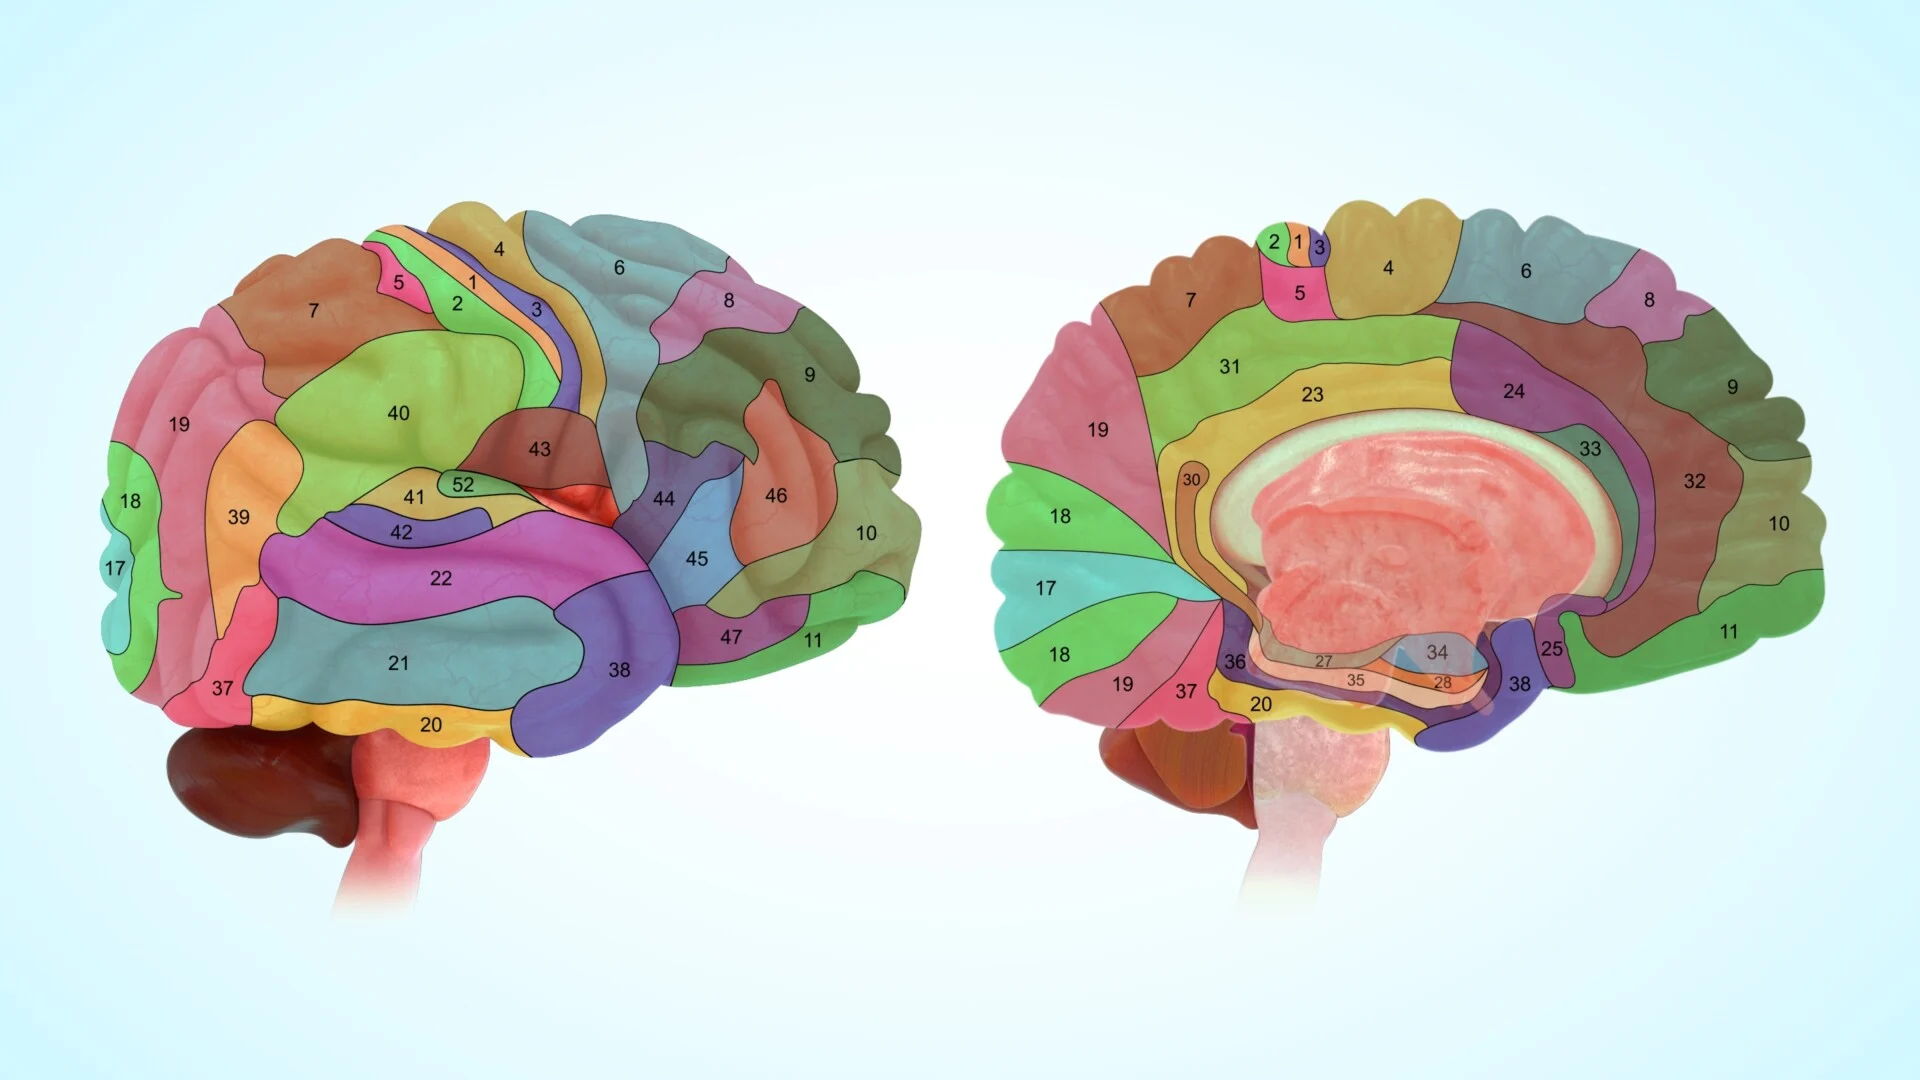
\includegraphics[width=0.6\textwidth]{images/BrodmannAreas.png}
\end{figure}
Functional specialization is exemplified by \textbf{retinotopic mapping} in the visual cortex, which transforms retinal images into a direct map in V1. Visual input is bifurcated so that stimuli from one visual field are processed by the \textbf{contralateral} brain regions, where parallel neuronal families independently analyze shape, movement, and color. \bigskip

Similarly, \textbf{somatotopic mapping} organizes the motor (pre-central gyrus, Area 4) and somatosensory (post-central gyrus, Areas 3, 1, 2) cortices. This is illustrated by the \textbf{Penfield Homunculus}, where cortical representation is proportional not to physical size, but to the density of sensory receptors and the complexity of motor control. Areas requiring high precision, such as the hands and face, occupy disproportionately large cortical territories compared to the torso. \bigskip
\begin{figure}[H] 
     \centering
     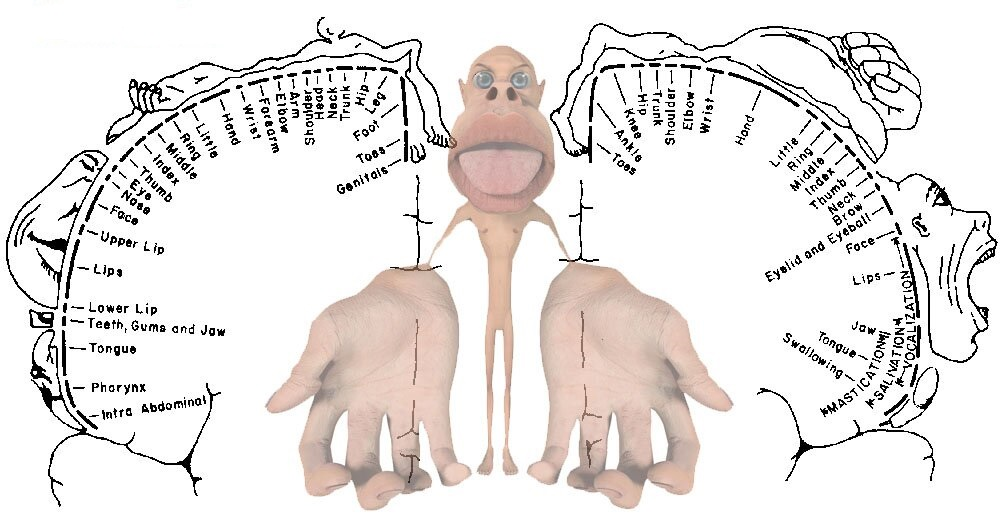
\includegraphics[width=0.6\textwidth]{images/homunculus.jpg}
     \caption{The Penfield Homunculus.}
\end{figure}
\begin{figure}[H]
  \centering
  \begin{minipage}{0.4\textwidth}
    \centering
    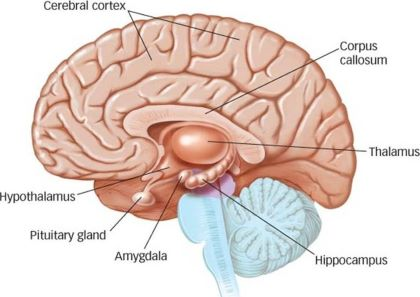
\includegraphics[width=0.9\textwidth]{images/subcortical.jpg}
  \end{minipage}
  \hfill
  \begin{minipage}{0.5\textwidth}
    Beneath the cortex lie \textbf{subcortical areas}—including the thalamus, brainstem, basal ganglia, and cerebellum—which are evolutionarily ancient regions responsible for survival and emotional regulation. The \textbf{thalamus} serves as a sophisticated relay station, directing sensory afferents to the cortex. Although deeply integrated with cortical networks, these structures pose a major challenge for neuroengineering: their depth makes measuring and monitoring their activity via non-invasive methodologies exceedingly difficult.
  \end{minipage}
\end{figure}
The brain's spatial organization is a multi-level hierarchy spanning from micrometers to centimeters. At the granular level, neural \textbf{layers} define the cytoarchitecture, which integrates into \textbf{cortical columns} as fundamental functional units. These columns form specialized \textbf{Brodmann areas} governing specific domains, which finally interconnect into complex \textbf{circuits}. This nested architecture ensures that while tasks are localized, the brain operates as a globally integrated system through predictive and generative models.
\begin{figure}[H] 
     \centering
     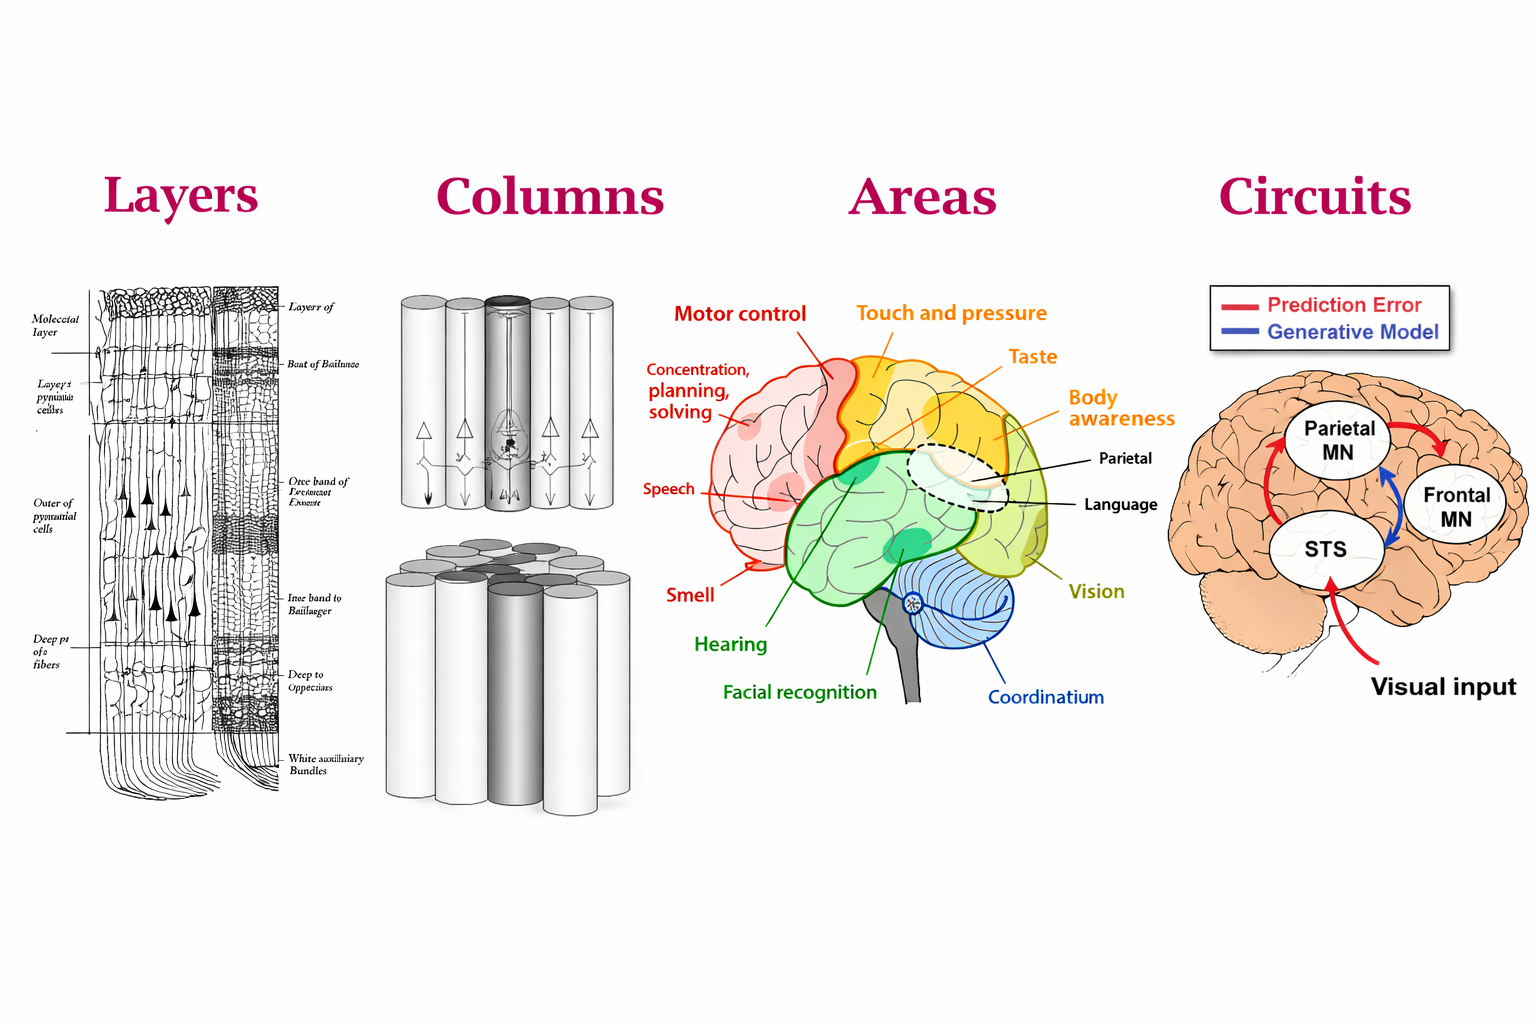
\includegraphics[width=0.5\textwidth]{images/brainStructure.png}
\end{figure}

\section{Brain Plasticity}\label{Plasticity}
\textbf{Brain plasticity} is the organ's ability to modify it's structure and function based on experience, a concept first hypothesized by William James in 1890. In 1949, Donald Hebb formalized this through \textbf{Hebbian Learning}, governed by the principle: ''cells that fire together, wire together.'' This theory states that repeated simultaneous activation of neurons increases \textbf{synaptic efficiency}, reinforcing neural pathways. This physical adaptation serves as the biological foundation for learning, habit formation, and memory throughout the lifespan.\bigskip

Neural plasticity evolves throughout the lifespan, peaking during the \textbf{critical period} (ages 0--2) when fundamental, often irreversible, connections are formed. While most potent in youth—enhancing the efficiency of neurorehabilitation—plasticity persists into adulthood and seniority through learning and memory consolidation. This adaptability is further evidenced by functional reorganization following \textbf{sensory deprivation} or limb loss. Ultimately, the brain's lifelong capacity to restructure in response to lesions or physiological changes provides the foundational principle for clinical neurorehabilitation.\bigskip

Plasticity mechanisms vary by temporal scale: while neurogenesis is mostly limited to the critical period, \textbf{synaptic plasticity} persists throughout life, governed by neurotransmitter release and postsynaptic receptor density.
\begin{figure}[H] 
     \centering
     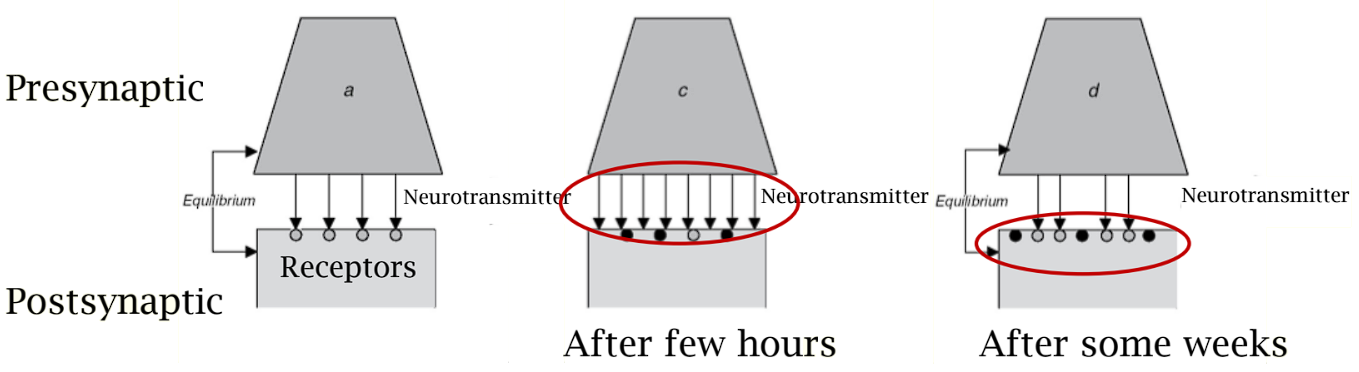
\includegraphics[width=0.8\textwidth]{images/plasticity.png}
\end{figure}
Short-term practice leads to \textbf{functional facilitation}, a transient increase in neurotransmitter release that enhances synaptic effectiveness without anatomical changes. Conversely, consistent long-term repetition induces \textbf{structural plasticity}, involving physical modifications such as increased receptor density. These stable anatomical changes provide the biological basis for long-term skill retention and expertise.\bigskip 

Plasticity also involves architectural changes through \textbf{axonal sprouting} (forming new synapses) and \textbf{pruning} (selective removal of redundant ones). During early development, the brain undergoes massive ''over-sprouting,'' which is metabolically unsustainable. Consequently, between ages 2 and 10, extensive \textbf{synaptic pruning} occurs. This is an optimization strategy rather than a loss of information: by eliminating unnecessary connections, the brain maximizes metabolic efficiency and ensures high-performance processing without excessive energy consumption.
\begin{figure}[H] 
     \centering
     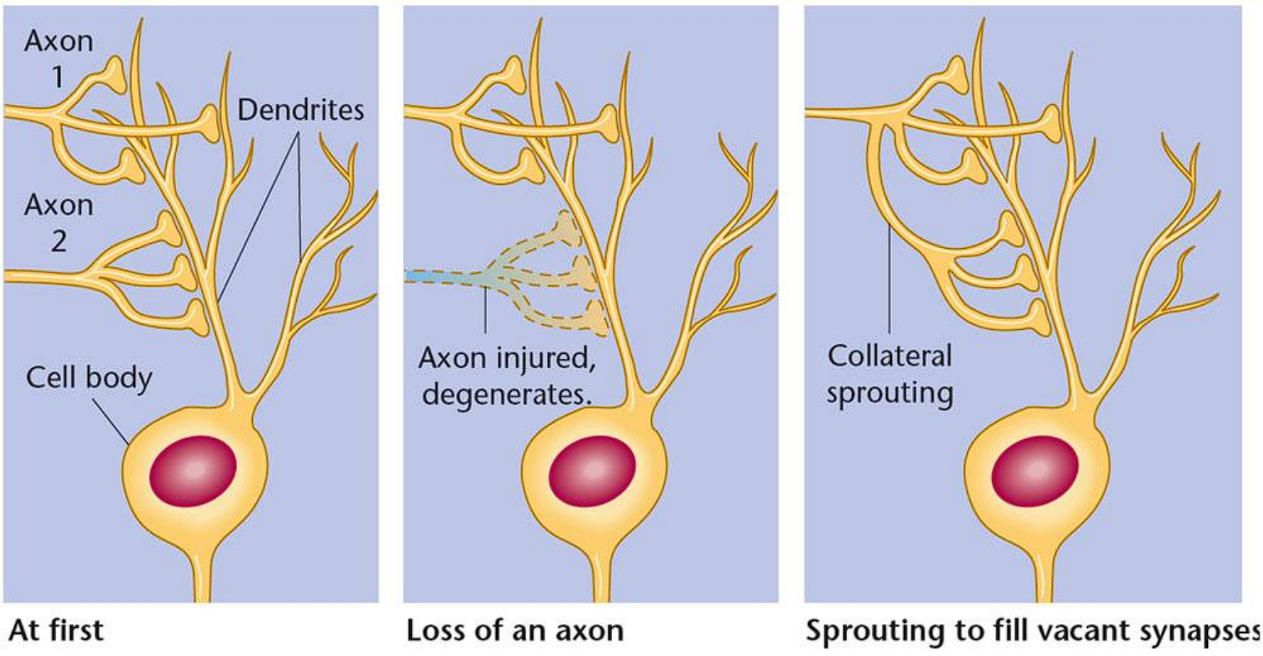
\includegraphics[width=0.7\textwidth]{images/reconstructionAxon.png}
\end{figure}
\textbf{Axonal regeneration} is a critical but limited recovery mechanism, primarily associated with early development. In the event of a lesion, the process begins with \textbf{Wallerian degeneration}, where macrophages clear the distal axon segment. Subsequently, \textbf{Schwann cells} align to form a guiding pathway for the slow regrowth of the axon toward it's target. Unlike rapid functional adaptations, successful reinnervation is a complex biological repair that can span months or years.
\begin{figure}[H] 
     \centering
     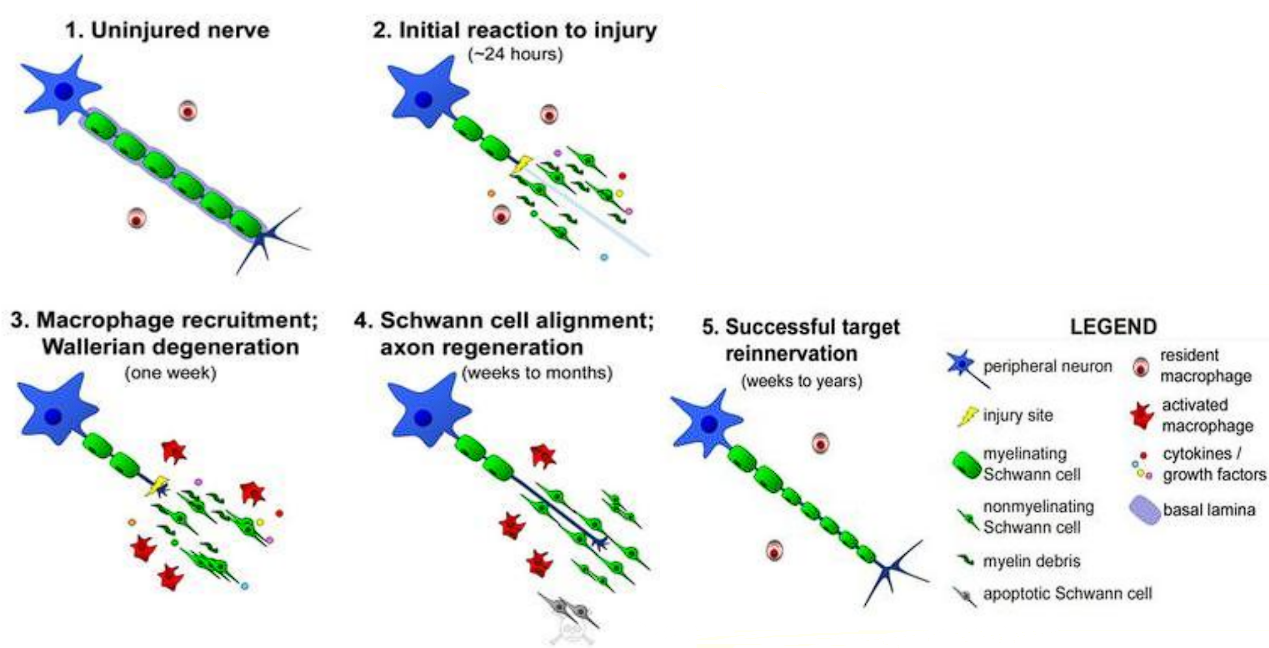
\includegraphics[width=0.7\textwidth]{images/axonal_regeneration.png}
\end{figure}
\begin{figure}[H]
  \centering
  \begin{minipage}{0.4\textwidth}
    \centering
    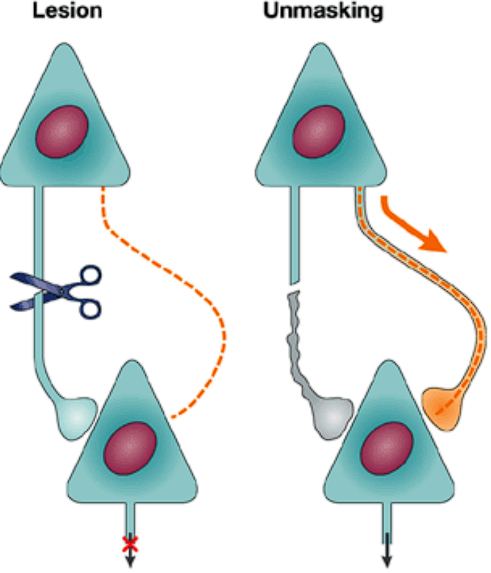
\includegraphics[width=0.8\textwidth]{images/unmasking.png}
  \end{minipage}
  \hfill
  \begin{minipage}{0.5\textwidth}
    \textbf{Neural redundancy} involves latent, inactive synaptic connections that serve as a functional backup. When a primary pathway is disrupted by a \textbf{lesion}, these dormant circuits are activated through a process called \textbf{unmasking}. Unlike the slow timeline of axonal regeneration, unmasking allows for rapid functional compensation by utilizing pre-existing structural over-provisioning, demonstrating the brain's inherent resilience to damage.
  \end{minipage}
\end{figure}
\chapter{Signals, Encoding and Decoding}
\section{Electrical Correlates of the Brain Activity}
Neuroengineering techniques for monitoring brain activity are governed by a trade-off between spatial resolution and invasiveness, spanning from direct Intracellular Potentials (IP) to non-invasive Electroencephalography (EEG). Intermediate approaches include Extracellular Potentials (EP), Local Field Potentials (LFP), Stereo-electroencephalography (S-EEG), and Electrocorticography (ECoG). Notably, while IP provides a direct measurement, the other listed methods capture only physiological correlates—phenomena influenced by, rather than equivalent to, actual brain activity.
\subsection{Single-Cell Recordings}
Intracellular recordings utilize hollow glass electrodes filled with an electrolyte, paired with a reference electrode placed in the extracellular medium. There are two primary techniques: sharp electrodes, which penetrate the membrane, and patch electrodes, which establish a seal on the membrane surface to contact the cell's interior. Although these methods are technically challenging to execute, they provide the most accurate measurement of actual membrane potential, offering exceptionally high temporal resolution.
\begin{figure}[H] 
     \centering
     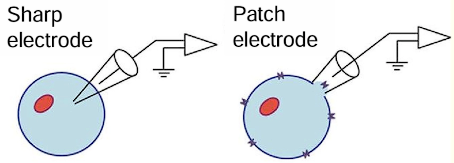
\includegraphics[width=0.4\textwidth]{images/sharp_path_electr.png}
\end{figure}
Intracellular recordings are technically more complex than extracellular methods and are typically conducted in in vitro experiments. They are primarily performed on the soma or dendrites to record graduate and action potentials, as capturing signals along the axon is notably difficult due to it's extreme thinness and the high risk of structural damage. Despite these technical challenges and the difficulty of maintaining precise measurements, this technique has been instrumental in advancing our fundamental understanding of cellular neurophysiology.\bigskip 

\textbf{Extracellular} recording involves positioning electrodes in the extracellular fluid near the cell membrane to monitor neural activity. While this method cannot detect subtle sub-threshold voltage changes or waveform details, it is highly effective at identifying the exact timing of action potentials. It is particularly valuable for in vivo studies, as it allows for reliable event detection without disrupting the cell's natural environment.

The intracellular recordings captures the subthreshold and the action potentials, the extracellular records a signal temporally correlated with the action potential.
\begin{figure}[H] 
     \centering
     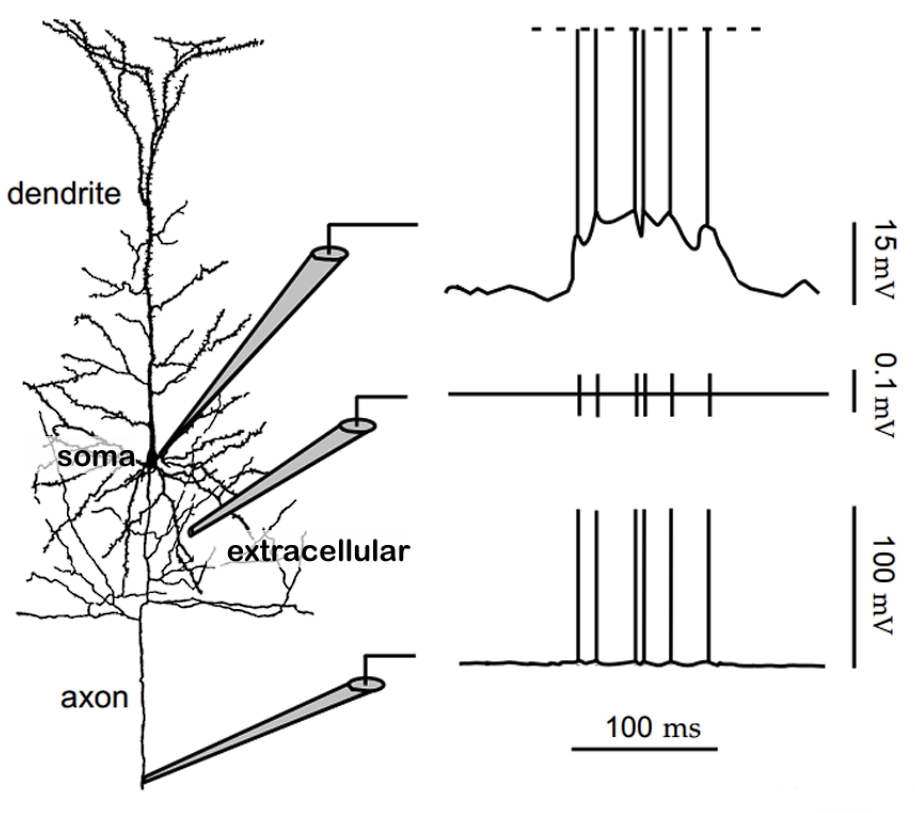
\includegraphics[width=0.4\textwidth]{images/intraextrarec.png}
\end{figure}
\subsection{Recordings from Neural Population}
\textbf{Local Field Potentials} (LFPs) represent the aggregate electrical activity within a local tissue volume, specifically reflecting the summation of postsynaptic potentials rather than individual action potentials. These signals are characterized by low-frequency oscillations, typically below 300 Hz. Because they capture the synchronized activity of neural populations and reflect regional inputs, LFPs serve as a critical tool for investigating large-scale circuit dynamics and neural oscillations within the brain.
\bigskip 

Electroencephalography (EEG) operates at a macroscopic scale, recording the synchronous postsynaptic activity of large populations of neurons. By utilizing the principle of volume conduction—where electrical fields propagate through brain tissue, cerebrospinal fluid, and the skull—EEG enables the non-invasive measurement of neural activity from the scalp. While this technique provides exceptional temporal resolution for investigating global brain dynamics, the summation of signals across diverse cortical regions significantly limits it's spatial precision compared to localized recording methods.
\begin{itemize}
     \item \textbf{Stereo-Electroencephalography (S-EEG)}: Invasive way to record the neuron activity with electrodes placed inside the brain, the spatial resolution is quite high, the weakness is that the surgeon has to make holes on the skulls, so this is not done routinely, since it would require a surgery only to acquire data, so is ethically allowed only when it's in the interest of the patient. The most common application of this is epilepsy.
     \begin{figure}[H] 
          \centering
          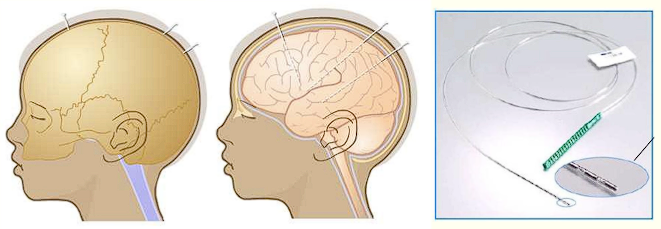
\includegraphics[width=0.6\textwidth]{images/SEEG.png}
     \end{figure}
     \item \textbf{Electrocorticography (ECoG)}: This method is similar but focused on the cortex, is slightly less invasive since requires the electrodes to be put on the cortex, it can be very detailed. The subcortical activity is spread through the head so this method measure both cortical (more clearly) and subcortical activity. The advantages of this measure is the spatial resolution and is clear the activity of the cortex. As cons, is invasive and is focused on specific regions (not all the brain).
     \begin{figure}[H] 
          \centering
          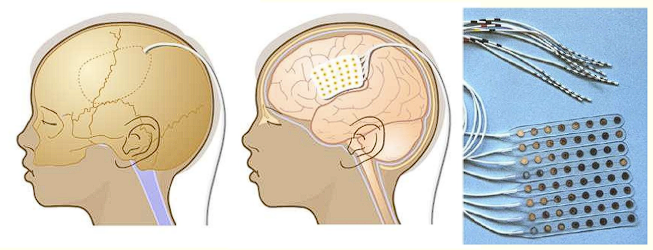
\includegraphics[width=0.6\textwidth]{images/ECoG.png}
     \end{figure}
     \item The \textbf{scalp EEG} is the only method that is completely non invasive, since the electrodes are just placed on the scalp, the first measurement of electrical signals from the scalp occurred in 1929 by the German psychiatrist Hans Berger. The easiest signal to detect through this method is the alpha rhythm.
\end{itemize}
The quality of the scalp EEGs acquired in the last century was not much different to the actual registrations.
\begin{figure}[H] 
          \centering
          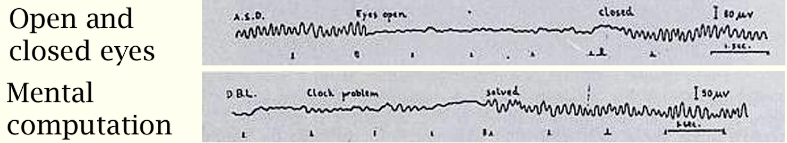
\includegraphics[width=0.6\textwidth]{images/1929.png}
\end{figure}
\subsection{Generation of the EEG Signals}
The \textbf{pyramidal neurons} are named for their pyramid-shaped soma and possess both apical and basal dendrites, with the apical dendrites extending towards the cortical surface. Importantly, these neurons are arranged in parallel groups called ''palisades'' that are oriented perpendicular to the surface of the cortex. This specific alignment and structure are fundamental for the generation of EEG signals.
\begin{figure}[H] 
          \centering
          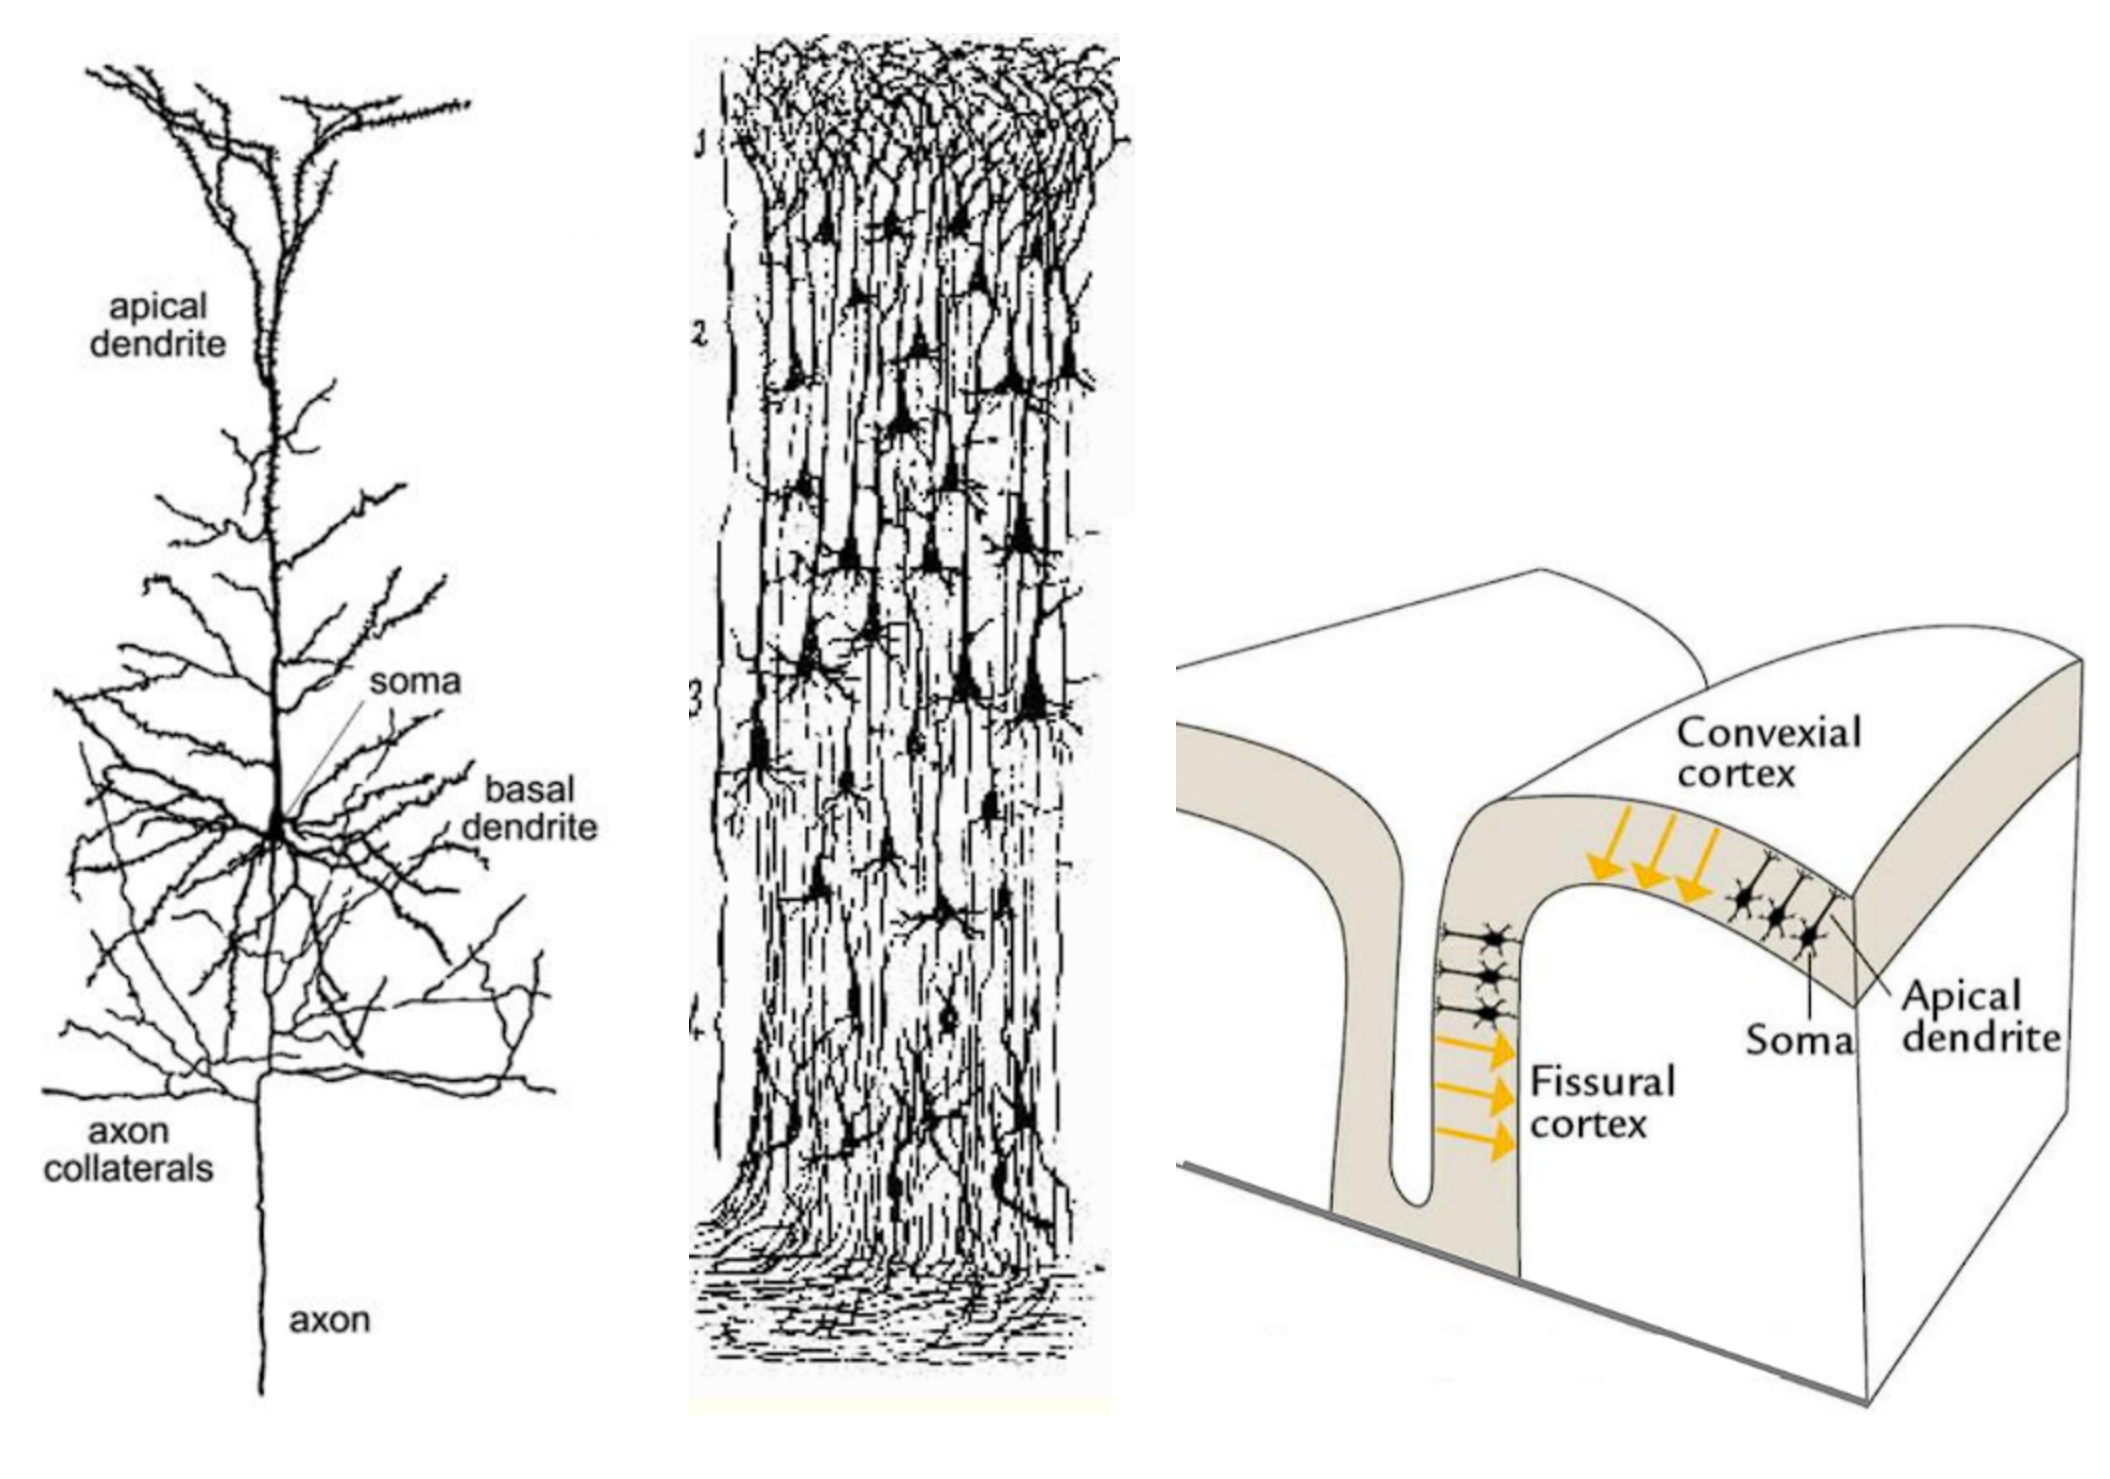
\includegraphics[width=0.6\textwidth]{images/pyramidalNeurons.eps}
\end{figure}
The neural electrical activity functions like a ''current dipole'', which is essential for understanding how brain signals are captured by EEG. When synapses are active, they cause local changes in electrical charge, creating both intracellular and extracellular ''return'' currents. These currents generate a dipole potential field that is strong enough to be detected at a distance, such as on the scalp. However, because a single neuron produces a very weak signal, the EEG readings we observe are the result of the combined, synchronized activity of many neurons rather than a single one.
\begin{figure}[H] 
          \centering
          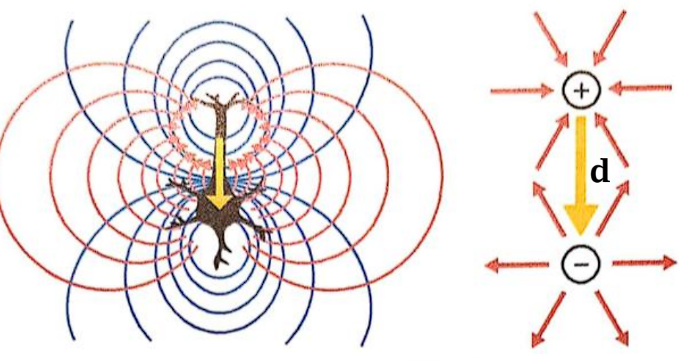
\includegraphics[width=0.4\textwidth]{images/dipole.png}
\end{figure}
The apical and basal dendrites function as a ''point source'' and ''sink'' for electrical current. Furthermore, the extracellular charges and currents are the reverse of the intracellular ones. The orientation of this dipole is not fixed; if the input synapse is inhibitory, the resulting dipole is reversed.
\begin{figure}[H] 
          \centering
          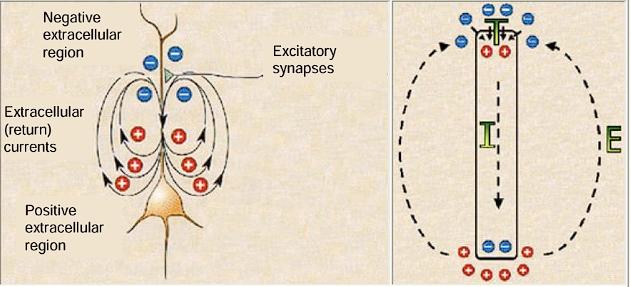
\includegraphics[width=0.45\textwidth]{images/dipole2.png}
\end{figure}
\begin{figure}[H] 
          \centering
          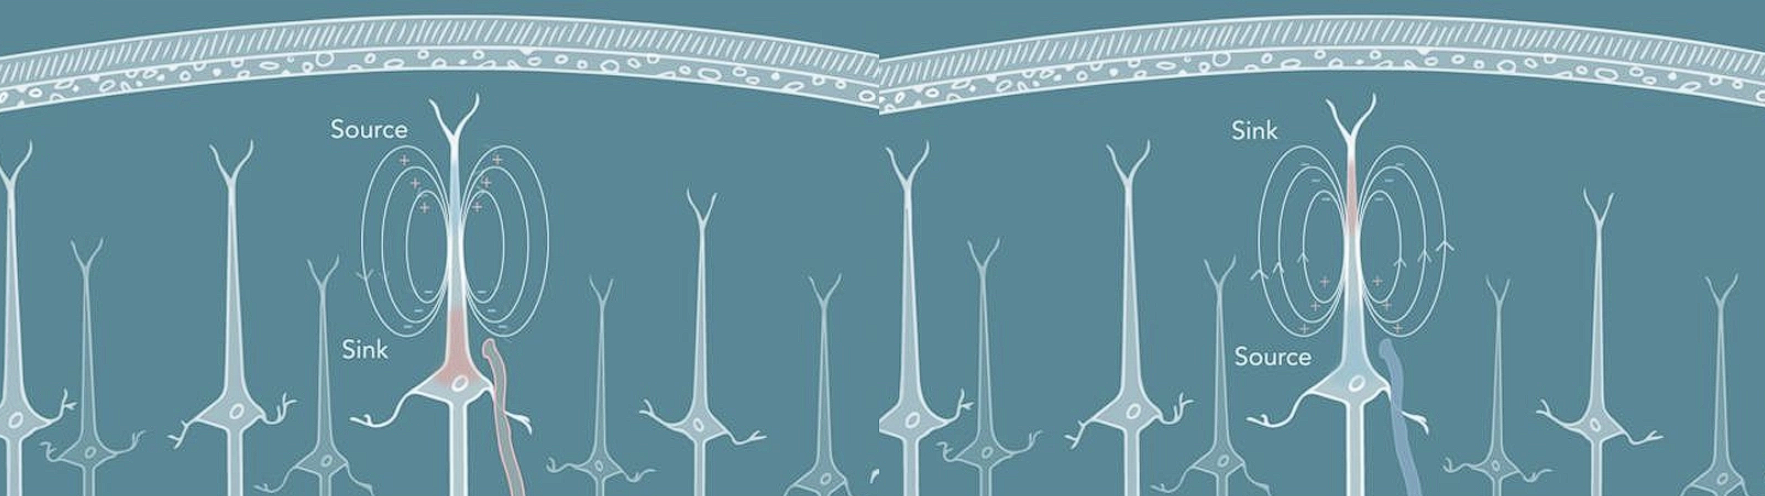
\includegraphics[width=0.6\textwidth]{images/source_sink.png}
\end{figure}
The direction of the dipole depends on where the synapses contact the neuron:\begin{itemize}
     \item \textbf{talamo-cortical (TC)}: these connection comes for the talamo, they connect directly with the basal dendrite. 
     \item \textbf{cortical-cortical (CC)}: these comes from the cortex, these connections tends to connect to the apical dendrite, since the contact point is far from the cell body, the resulting dipole has a different orientation than that generated by the thalamic input.
\end{itemize}
\begin{figure}[H] 
          \centering
          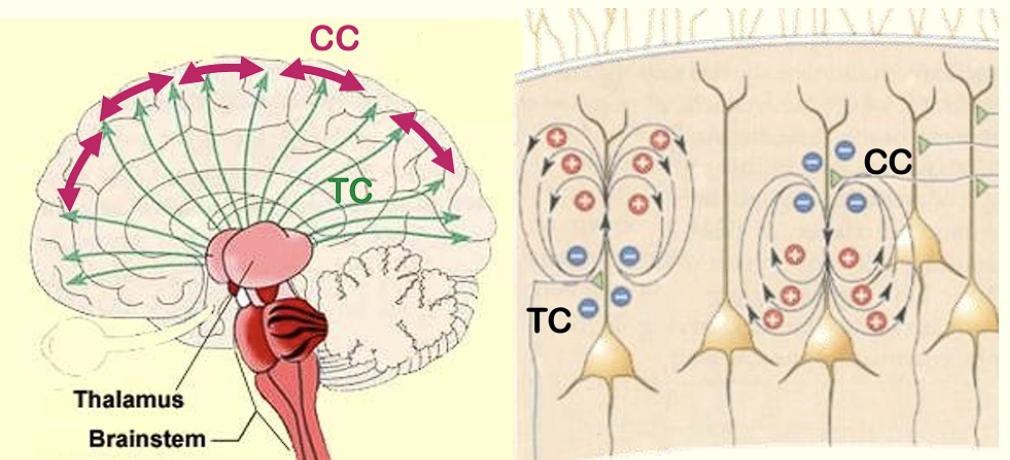
\includegraphics[width=0.6\textwidth]{images/TC_CC.png}
\end{figure}
Because the cortex's pyramidal neurons are aligned parallel to each other, when many neurons receive the same type of input simultaneously, their small dipoles add up. If the dipoles were disordered, they would cancel each other out. Thanks to this neat geometric organization, the signals become strong enough to be detected by electrodes placed on the scalp.\bigskip 

To determine the direction of the dipole, the nervous system combines two factor:\begin{itemize}
     \item Nature of the synapse: inhibitory or excitatory.
     \item Position of the synapse: CC or TC.
\end{itemize}
\begin{table}[H]
     \centering
\begin{tabular}{l|l|l|}
\cline{2-3}
                        & CC   & TC   \\ \hline
\multicolumn{1}{|l|}{E} & down & up   \\ \hline
\multicolumn{1}{|l|}{I} & up   & down \\ \hline
\end{tabular}
\end{table}
Despite they exists four different configurations, we can observe only two results (up or down direction). If a scalp electrode detects an ''up'' oriented dipole, it cannot know for sure whether it is caused by an excitatory TC input OR an inhibitory DC input.\begin{quote}
     \textbf{Conclusion}: The same signal measured externally can be produced by profoundly different cellular mechanisms.
\end{quote} 

The EEG is much more sensitive to activity that occurs in the gyri  than that that occurs in the sulci:\begin{itemize}
     \item \textbf{Gyri}: Their orientation is ''favorable'', because the top of the gyrus faces directly toward the scalp, the dipole is oriented perpendicular to the surface of the skull. This creates an electrical potential that points straight towards the electrode.
     \item \textbf{Sulci}: Here a physical problem arises. Neurons in the sulci are oriented ''sideways'' (tangentially) to the surface of the skull. Furthermore, because the sulcus is made up of two opposite walls, the neurons on the left wall point to the right and those on the right wall point to the left. The dipoles of the two opposite walls of the groove tend to cancel each other out (vector sum close to zero).
\end{itemize}
\begin{figure}[H] 
          \centering
          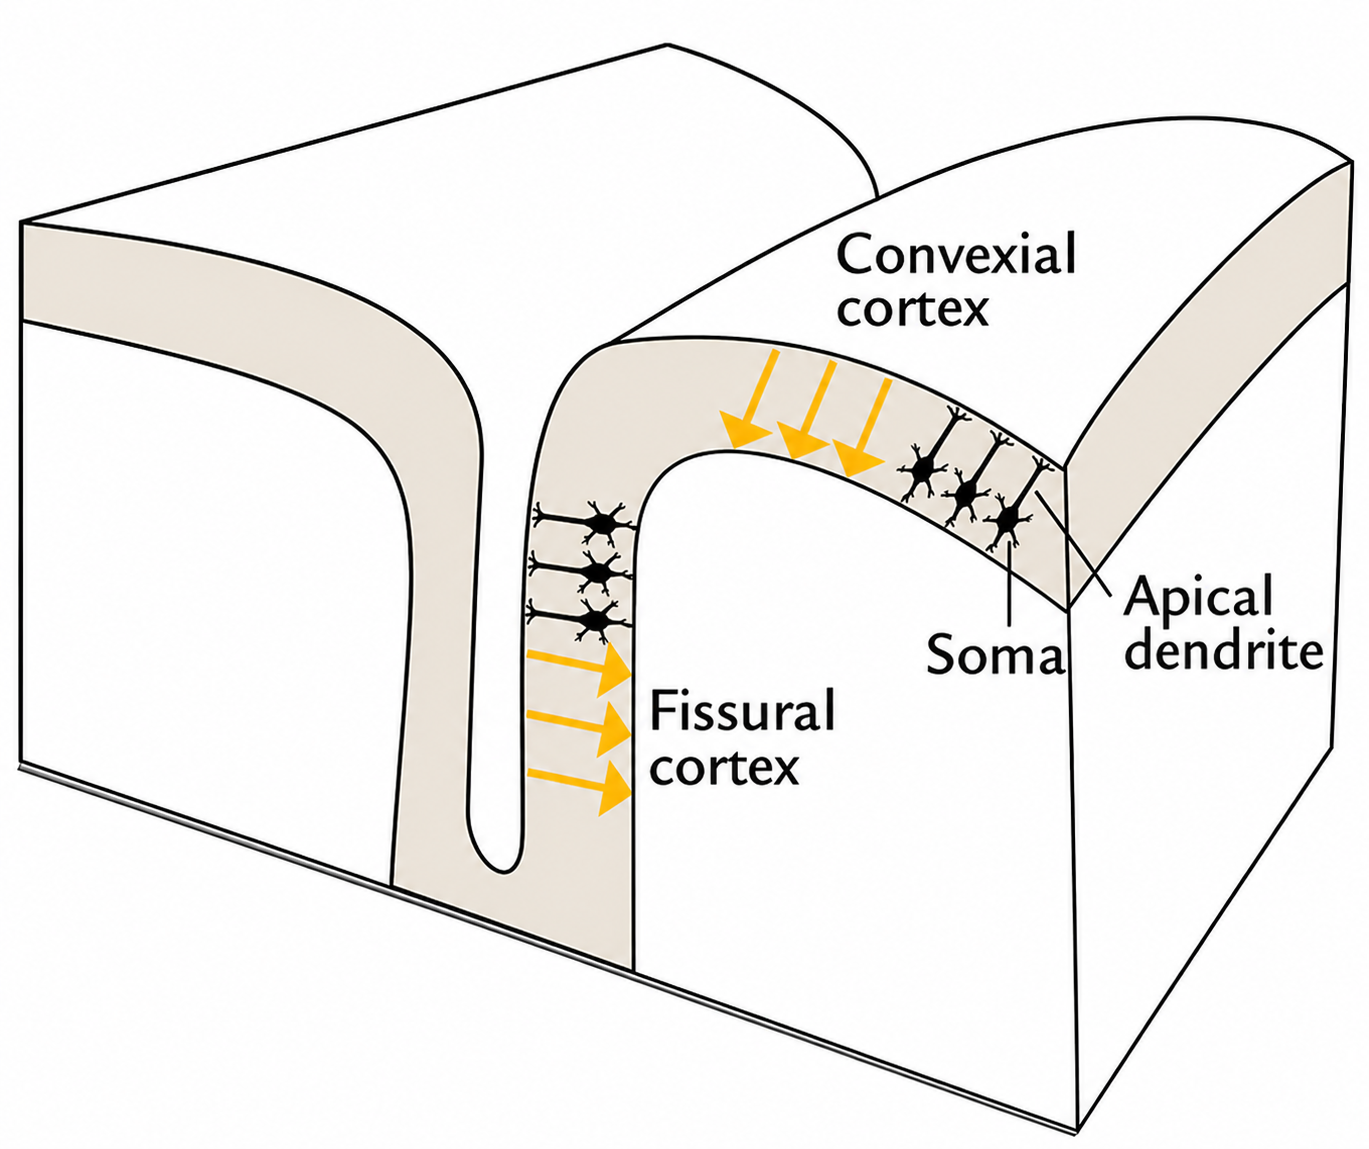
\includegraphics[width=0.4\textwidth]{images/gyrysulci2.png}
\end{figure}
Furthermore, the sulci are deeper. Since the electric field decays with the square (or cube, depending on the model) of the distance, being deeper means that the signal reaches the scalp much more attenuated.\bigskip 

The EEG doesn't simply measure the brain activity, but the \textbf{synchronized activity}:\begin{itemize}
     \item If millions of neurons fire at random times, their electric fields cancel each other out (destructive interference). The resulting signal is minimal. In this situation the signal is proportional to the square root of the number of neurons that are firing. 
     \item When neurons ''agree'' and fire at the same time (constructive interference), the signal becomes proportional to the linear number of neurons.
\end{itemize}
The electrical signal on the EEG is huge not because there are ''more'' active neurons, but because they are \textbf{coordinated}. Synchrony acts as a natural amplifier. As already mentioned, sulci produce little or no EEG signals, the orientation is not favorable to the scalp surface, the gyri produce most of the EEG signal, thanks to the summation due to the palisade disposition.\bigskip 

To determine if the signal produced by the neurons will reach the electrode, we introduce the concept of closed and open field:\begin{itemize}
     \item A \textbf{closed field} is produced by neurons that have a symmetric or radial structure, even if the neurons are active, if they are asynchronous the signal received is practically null, the electric field is ''trapped'', and the signal can't reach the scalp.
     \item When the neurons are in a pyramidal structure, parallel aligned and synchronized, their electric dipoles add constructively (\textbf{open field}). The electric field propagates outward, making the signal measurable in the EEG.
\end{itemize}
As a resume, an open field is measurable by the EEG on the scalp, instead a closed field do not reach the scalp.\bigskip 

\noindent Now the question is: \textit{What are we measuring when we observe an EEG trace?} The answer is that the EEG is almost exclusively the effects of post synaptic potentials (PSPs).

Because PSPs last much longer than action potentials (APs), it is much more likely that the activities of many different neurons overlap over time.

\subsection{Limitations and Advantages of the Scalp EEG}
The EEG is not a perfect way to measure the brain activity, but at the same time it is irreplaceable. The limitations of the EEG are the following:\begin{itemize}
     \item \textbf{Spatial Blur}: As the signal must pass through tissue, bone and skin, the potential lines ''spread out'' and become attenuated. It's like trying to understand who's speaking in a room through a closed door: the sound becomes muffled and less localizable.
     \item \textbf{Correlation and Overlap}: Because the electrodes are close together, they often measure the same background signal. This makes it difficult to understand which specific area the activity is coming from.
     \item \textbf{Reference Problem}: Every voltage measurement is relative. EEG measures the potential difference between an active electrode and a ''reference''. If the reference is not truly neutral (and there is no truly neutral point in the body), it contaminates the entire signal.
     \item \textbf{Deep Source}: As we have seen, neurons must be arranged in an ''open'' manner to be seen. Deep sources (subcortical structures) often generate closed fields or are too far away, being ''turned off'' by signal attenuation.
\end{itemize}
\begin{figure}[H] 
          \centering
          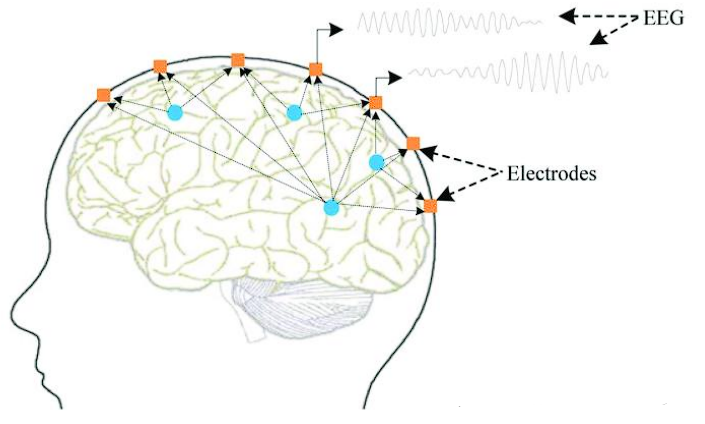
\includegraphics[width=0.4\textwidth]{images/LimitationEEG.png}
\end{figure}
Despite the limitations listed above, EEG remains the standard in many clinical and research fields for practical and technical reasons:\begin{itemize}
     \item \textbf{Temporal Resolution}:EEG has a temporal resolution of milliseconds. For studying the rapid dynamics of the brain, there is nothing better.
     \item \textbf{Practicality}: It is non-invasive, economical, portable and easy to use. It allows recording brain activity in real-life contexts or in patients where other technologies would be too cumbersome or dangerous.
     \item \textbf{Coverage}: It provides an overview of the entire cortical surface simultaneously, allowing the connectivity between different brain areas to be studied.
\end{itemize}
\section{Neural Encoding}
With \textbf{encoding} we describe the process of how an external stimuli (light, sounds) is transformed by the nervous system in a series of electrical signals. The \textbf{decoding} is the inverse process: we take the series of spikes (the raw data coming out of the brain) and try to reconstruct the original information.
\begin{figure}[H] 
          \centering
          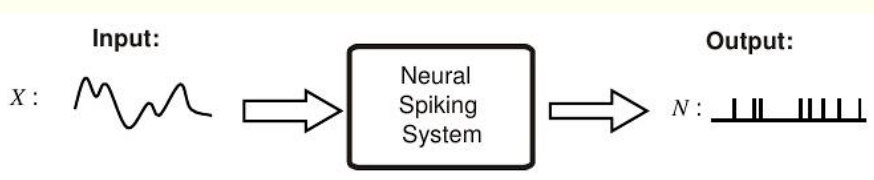
\includegraphics[width=0.6\textwidth]{images/encoding.png}
\end{figure}
Let $R$ to be the neural response, $S$ the stimulus and $f$ the function describing how the neural system respond to that stimulus:\begin{equation}
     R=f(S)
\end{equation}
Our goal is to find a mathematical model that approximate $f$, in that way we no longer need to test every single possibility. I can insert a new stimulus $S_{new}$ and predict (calculate) what the neuron's response $R$ will be. This is the ''Holy Grail'' of brain-computer interfaces (BCIs). The neural decoding is the inverse process\begin{equation}
     S=f^{-1}(R)
\end{equation}
that aim to find a model of $f^{-1}$. We will live under the assumption of \textbf{Rate-Coding Hypothesis}:\begin{itemize}
     \item Neurons communicate electrical ''shoots'' called action potentials (spikes).
     \item The content of the information is encoded in the frequency with which these spikes are repeated.
     \item More spikes in one second = More intense stimulus.
\end{itemize}
\begin{figure}[H] 
          \centering
          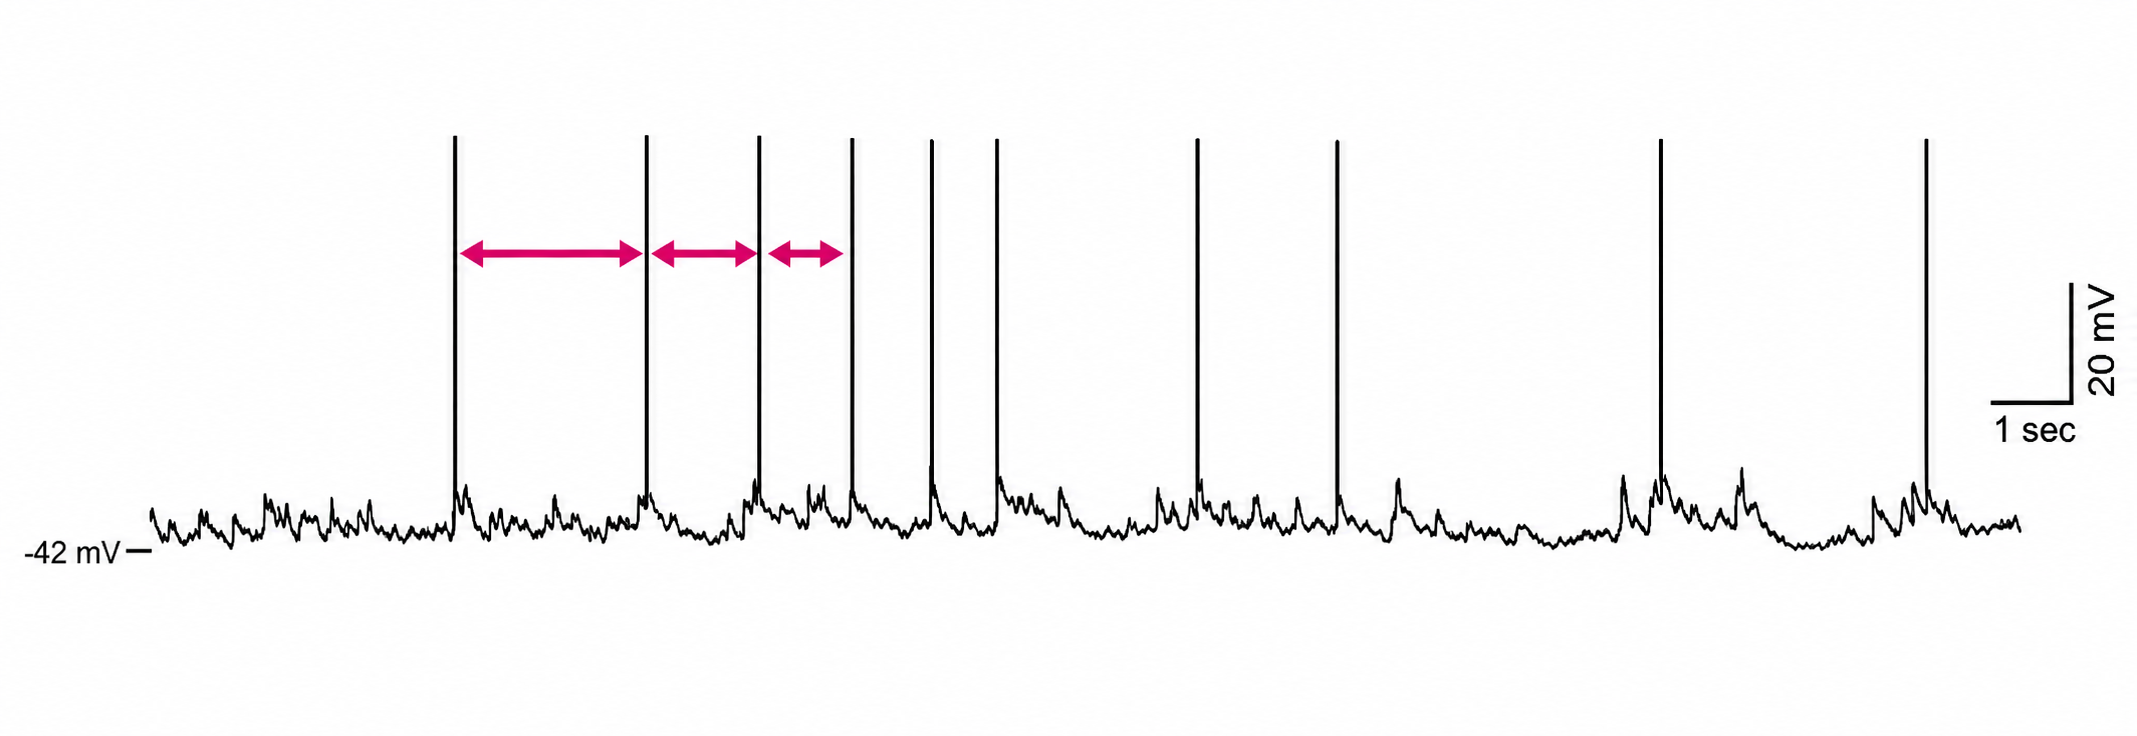
\includegraphics[width=0.6\textwidth]{images/firingNeurons.png}
\end{figure}
\begin{boxdefinition}{Spike Train}{}
     Let $\delta(t)$ to be the Dirac delta function, let $t_i$ to be the time in which the $i$-th spike of the $n$ total spikes occurred. The \textbf{spike train} is defined as follows:\begin{equation}
          \rho(t)=\sum_{i=1}^n\delta(t-t_i).
     \end{equation}
     $\rho$ is called \textbf{neural response function}.
\end{boxdefinition}
We recall that $\delta$ is defined\footnote{
     This is a ''practical'' and not formal definition of the Dirac delta, the formal definition requires theory of distributions.
} as the function null everywhere except on the origin, such that \begin{equation}
     \int_\R\delta(t)dt=1. 
\end{equation}
Suppose that we have recorded a spike train from time 0 to $T$, the number of spikes is given by\begin{equation}
     \int_0^T\rho(t)dt=n 
\end{equation}
and the \textbf{spike-count firing rate} is the time average of the neural response function over the duration of the trial:\begin{equation}
     r=\frac{n}{T}=\frac{1}{T} \int_0^T\rho(t)dt.
\end{equation}
When we analyze the data (spike train) we are not directly seeing the stimulus response, but the stimulus \textbf{filtered} by the biological property of the neuron. We have to make a distinction between different stimuli:\begin{itemize}
     \item \textbf{Stationary Stimulus}: If the stimulus is constant (e.g. a fixed light), the firing rate of the neuron is stable. In this case, you can simply count how many spikes occur in a time interval $T$ (the ''spike-count'').
     \item \textbf{Dynamic Stimulus}: If the stimulus changes quickly (e.g. a sequence of images or sounds), counting the spikes over a long period of time is useless, because you would ''spread'' the information and lose the quick details. In this case, a time-resolved definition is needed.
\end{itemize}
A single neuron is noisy and unreliable: We need to examine the relationships (correlations) between the discharge patterns of the entire population. If many neurons ''say'' the same thing at the same time, the signal becomes robust and the information is encoded with much more precision than a single cell would.\bigskip 

Neural responses can vary across repetitions (trials) even
when the same stimulus is presented repeatedly. We can't define a single rate $r$ to a stimulus, instead, we use a probabilistic approach, denoting $\langle r\rangle$ the \textbf{average firing rate} computed by averaging different trials.
\begin{figure}[H] 
          \centering
          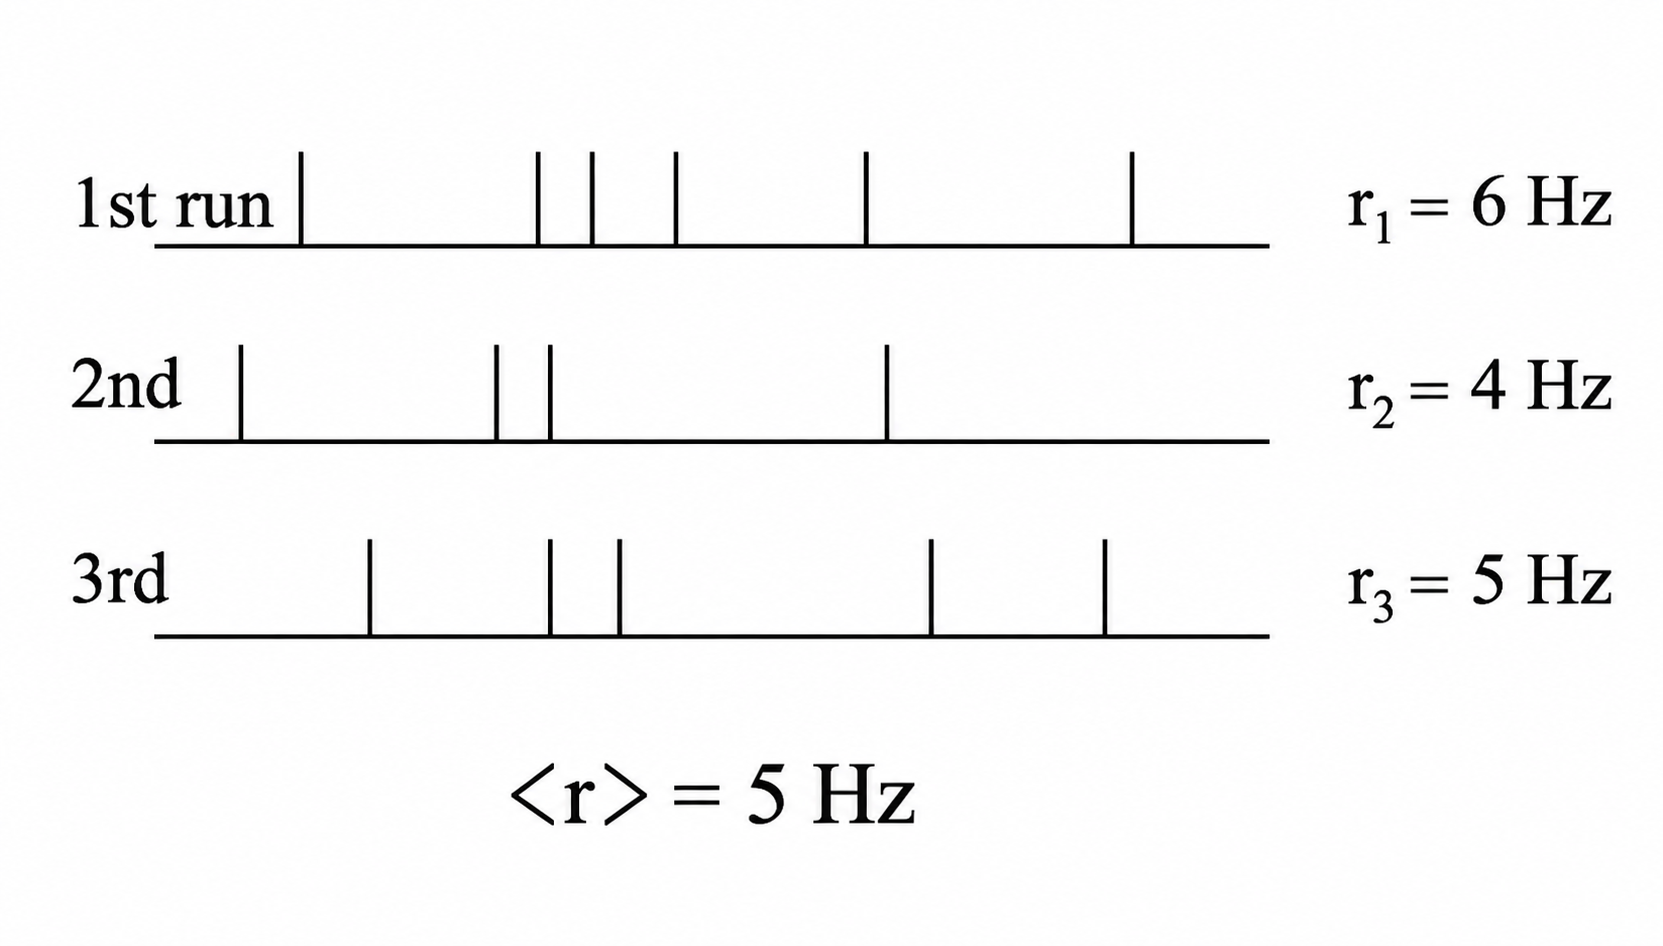
\includegraphics[width=0.5\textwidth]{images/averageRate.png}
\end{figure}
The brain does not treat all stimuli the same. A neuron in the visual cortex, for example, could fire lots of impulses when it sees a line oriented at 45 degrees, but remain almost silent if the line is horizontal.
\subsection{Tuning Curve}
The \textbf{Tuning Curve} is the mathematical function that describes this relationship: How much does the neuron fire ($y$-axis) in response to a given value of a stimulus property ($x$-axis)?\bigskip

We focus on a single property $s$ of a stimulus (for example, the degree of a line of light captured by the eyes), and define $f$ as the tuning curve of the neural response, that relates the average firing rate given the property $s$:\begin{equation}
     \langle r \rangle = f(s)
\end{equation}
we assume that $s$ is stationary along each trial.\bigskip


\noindent\textbf{Example 1}: An example of tuning curve is represented in Figure \ref{TunCurve}, in that case the analytic definition of $f$ is\begin{equation}
     f(s)=r_{max}\exp\left(
          -\frac{1}{2}\left(\frac{s-s_{max}}{\sigma_f}\right)^2
     \right).
\end{equation}
\begin{figure}
          \centering
          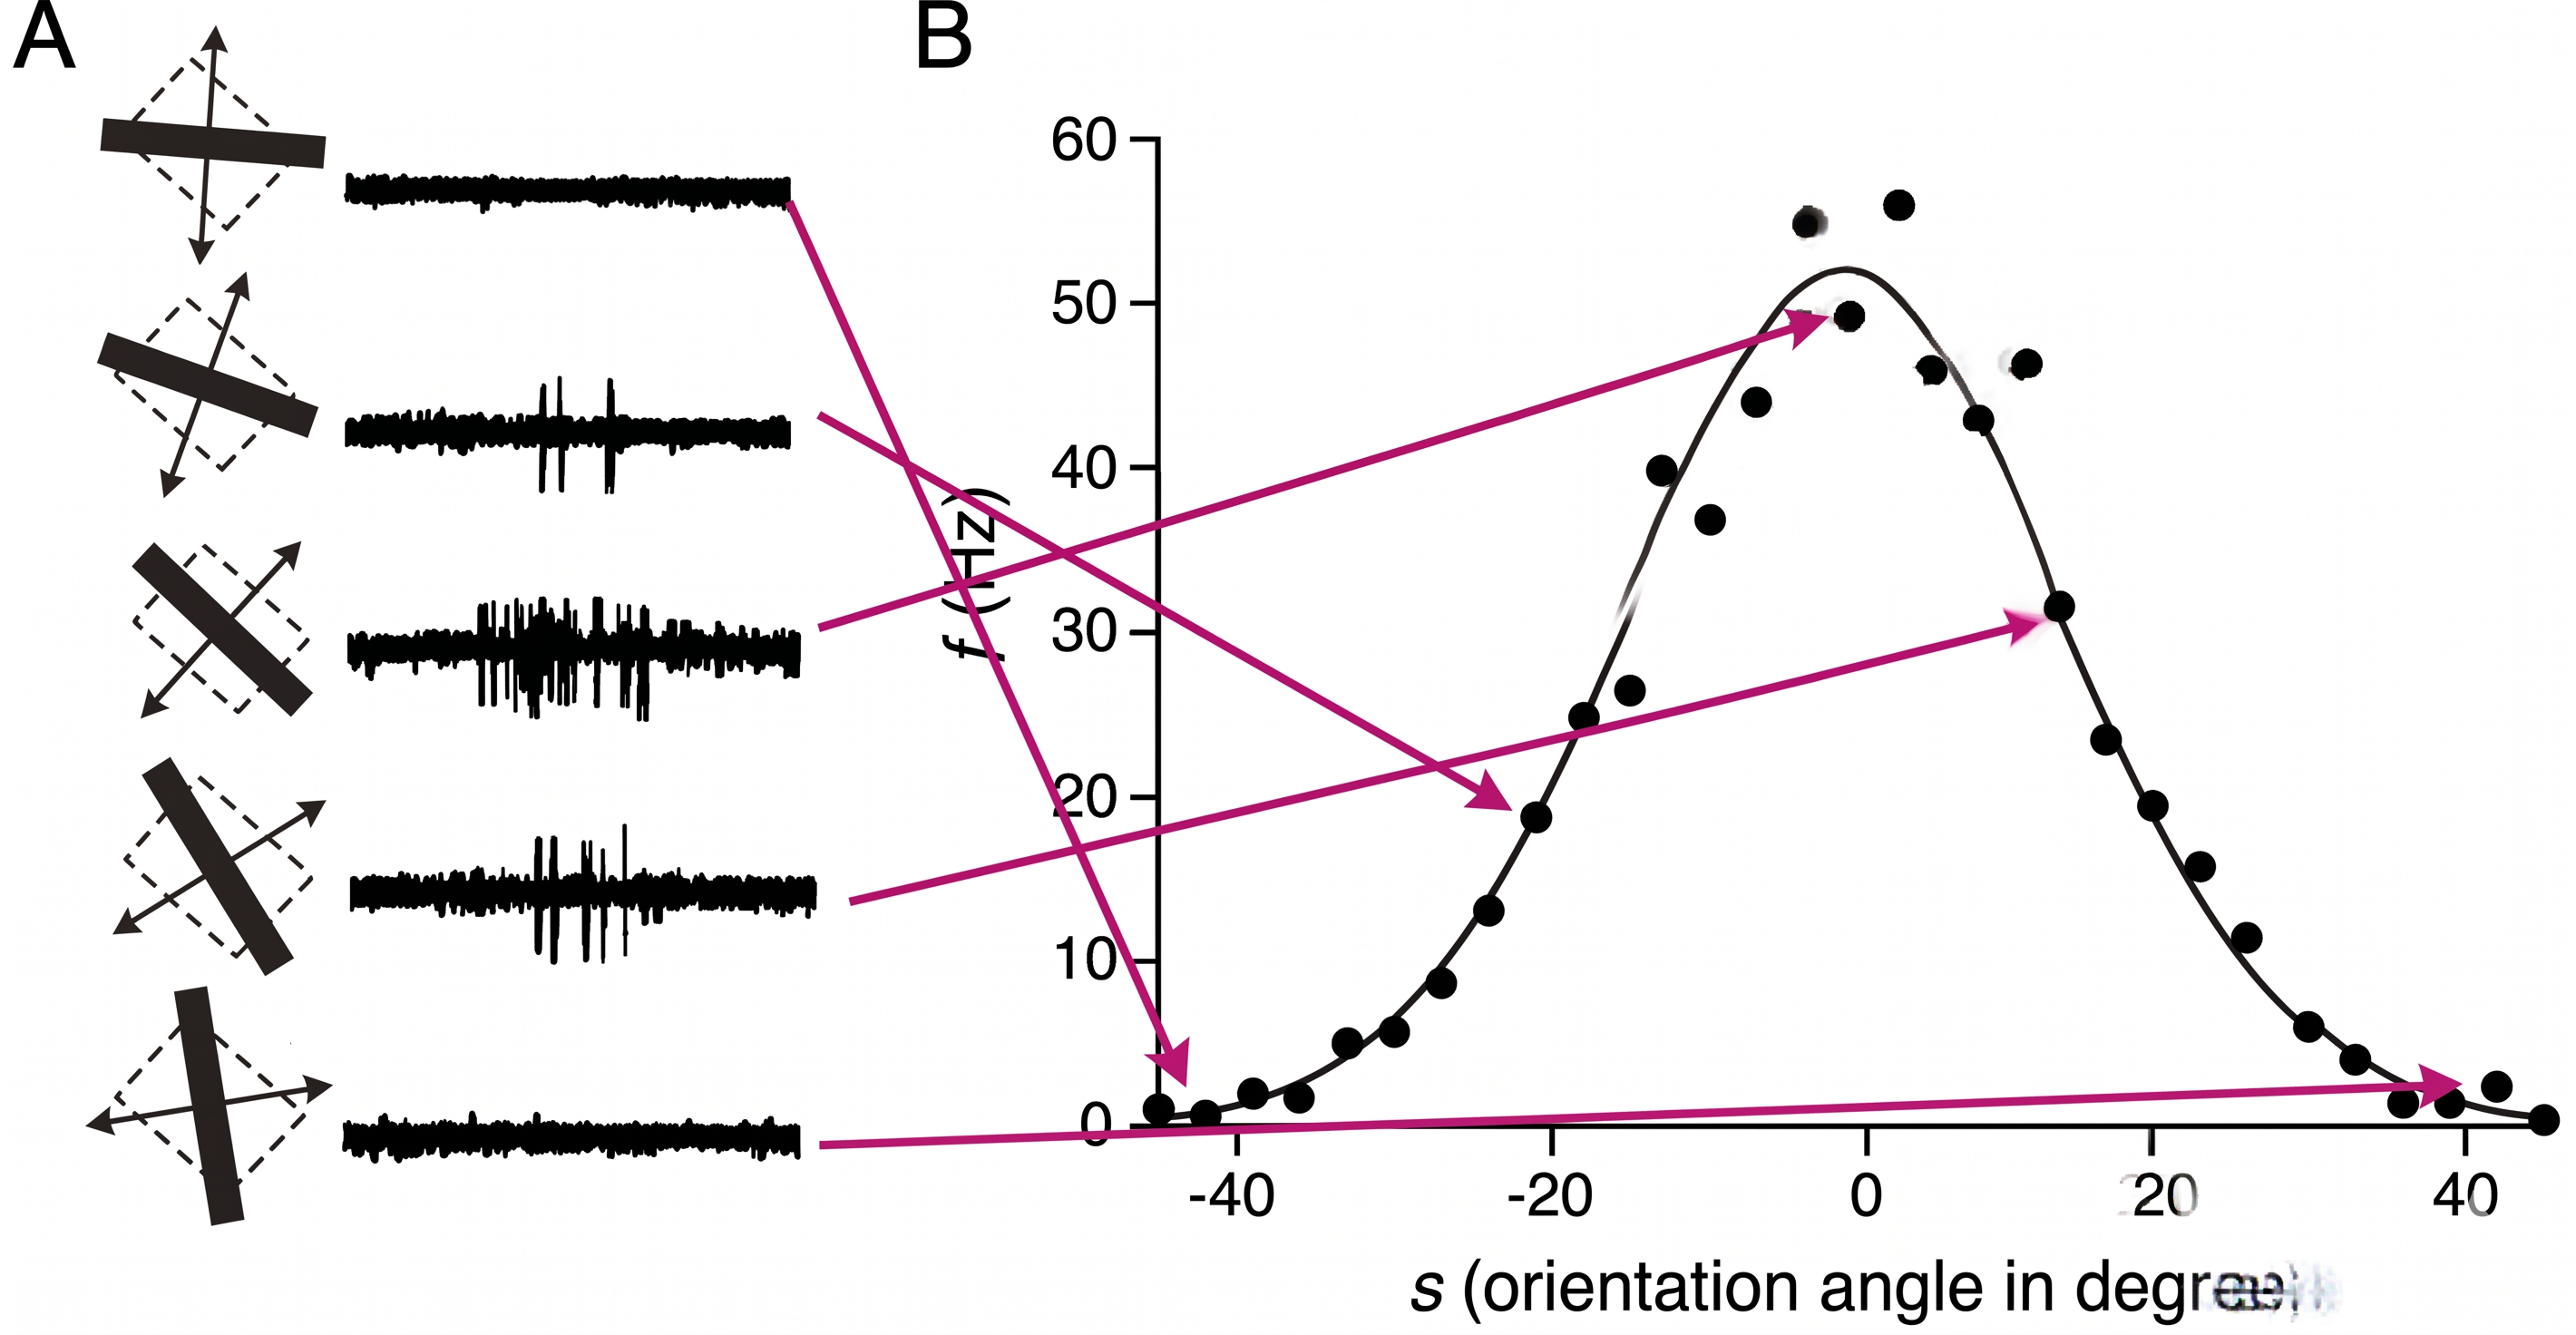
\includegraphics[width=0.55\textwidth]{images/tuningCurve.png}
          \caption{Example (1) of tuning curve.}
          \label{TunCurve}
\end{figure}
This curve have been estimated by experimentation on an animal subject (monkey) on the primary visual cortex, $s_{max}$ is the angle evoking the maximum response, and $\sigma_f$ is the amplitude of the tuning curve.\bigskip

\noindent\textbf{Example 2}: This example regards the neuron in the primary motor cortex of a monkey trained to reach in different directions. The firing rate of the cell is correlated with the direction of arm movement $s$ (in degrees). 
\begin{figure}
          \centering
          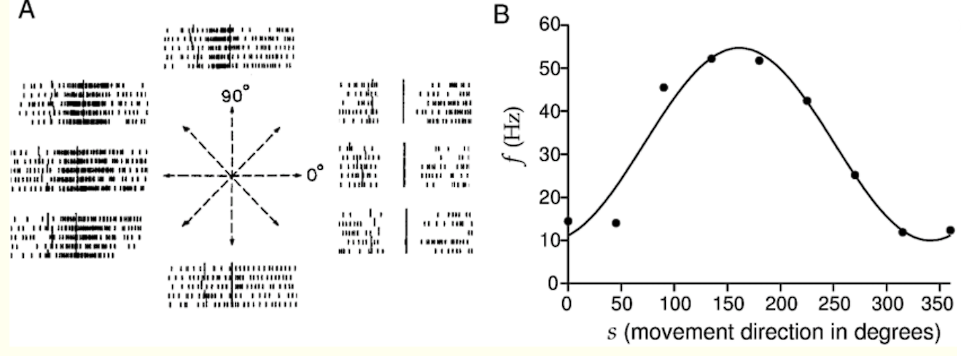
\includegraphics[width=0.8\textwidth]{images/tuningCurve2.png}
          \caption{Example (2) of tuning curve.}
          \label{TunCurve2}
\end{figure}
The curve shown in figure \ref{TunCurve2} is defined as follows:\begin{equation}
     f(s)=r_0+(r_{max}-r_0)\cos(s-s_{max})
\end{equation}
where $s_{max}$ is the angle evoking the maximum response, and $r_0$ is an offset to avoid negative firing rate.\bigskip

\noindent\textbf{Example 3}: This experiment is done on the primary visual cortex of a cat, reacting to \textit{retinal disparity} (a
difference in the retinal
location of an image
between the two eyes). The curve in figure \ref{TunCurve3} represent the tuning curve, where $s$ is the binocular retinal disparity in degrees, $\Delta_s$ controls how quickly the firing rate increases as a function of $s$ and $s_{\nicefrac{1}{2}}$ is the disparity inducing a response equal to $\frac{1}{2}$ of the maximum rate $r_{max}$.\begin{equation}
     f(s)=\frac{r_{max}}{1+\exp\left(
          \frac{s_{\nicefrac{1}{2}}-s}{\Delta_s}
     \right)}.
\end{equation}
\begin{figure}
          \centering
          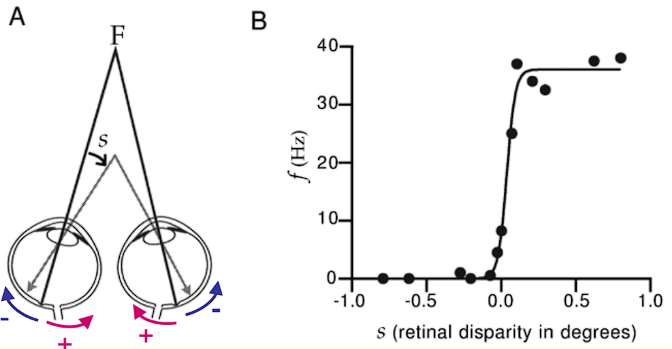
\includegraphics[width=0.5\textwidth]{images/tuningCurve3.png}
          \caption{Example (3) of tuning curve.}
          \label{TunCurve3}
\end{figure}
\subsection{The Poisson Spike Generator}
We want to build a stochastic model of the neuronal response. The Figure \ref{Hodgkin} represents the famous Hodgkin-Huxley model. It is an equivalent electrical circuit that perfectly describes the neuronal membrane:\begin{itemize}
     \item Each ion channel ($Na^+, K^+, Cl^-$, etc.) is modeled as a conductance (variable resistance) and a battery (reversal potential).
     \item To calculate exactly when a neuron fires an action potential, you would have to solve a system of nonlinear differential equations for every single bit of membrane on every single neuron in the network you are studying.
\end{itemize}
\begin{figure}[H]
          \centering
          \includegraphics[width=0.4\textwidth]{images/Hodgkin.png}
          \caption{Hodgkin-Huxley model.}
          \label{Hodgkin}
\end{figure}
To simulate an entire cortical network in this way is computationally impossible: We need a statistical model that allows us to estimate the
probability of an arbitrary spike sequence occurring, based on
our knowledge of the responses actually recorded.
\begin{figure}[H]
          \centering
          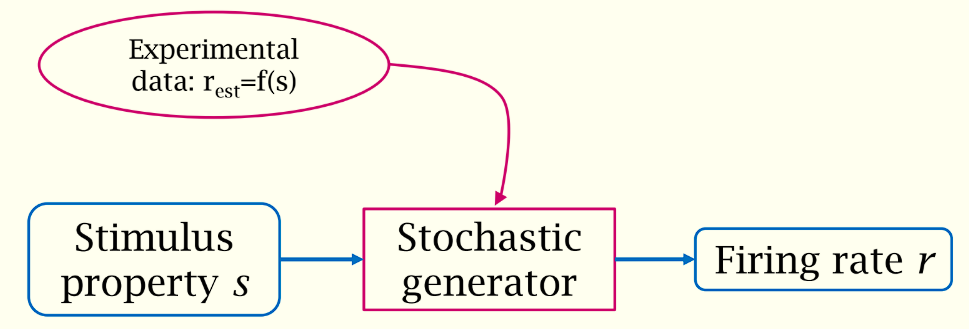
\includegraphics[width=0.5\textwidth]{images/stochGen.png}
\end{figure}
If the probability of generating an action potential is independent of the presence or timing of other spikes the firing rate $r$ is all we need to compute the probabilities for all possible action potential sequences.
Our statistical model is called \textbf{Poisson Process}:\begin{itemize}
     \item In biological reality, neurons have a ''refractory period'' (after a spike, the neuron needs an instant to ''recharge''). The Poisson model ignores this biological detail for simplicity. It's an approximation, but it's incredibly useful because it allows us to use very simple mathematical tools to calculate the probability of entire sequences of spikes.
\end{itemize}
We focus on the \textbf{homogeneous} model where the firing rate $r$ is constant over time. Imagine a neuron that, in a resting state, fires an average of 10 spikes per second. Since the rate is fixed, the probability calculation is immediate.\bigskip

We treat the action potentials as \textbf{discrete event}, a Poisson stochastic process produces an integer non-negative number of statistically independent events. We divide the trial duration $T$ in small intervals $\Delta t$ such that no more than a single spike occurs in a single interval.
\begin{figure}[H]
          \centering
          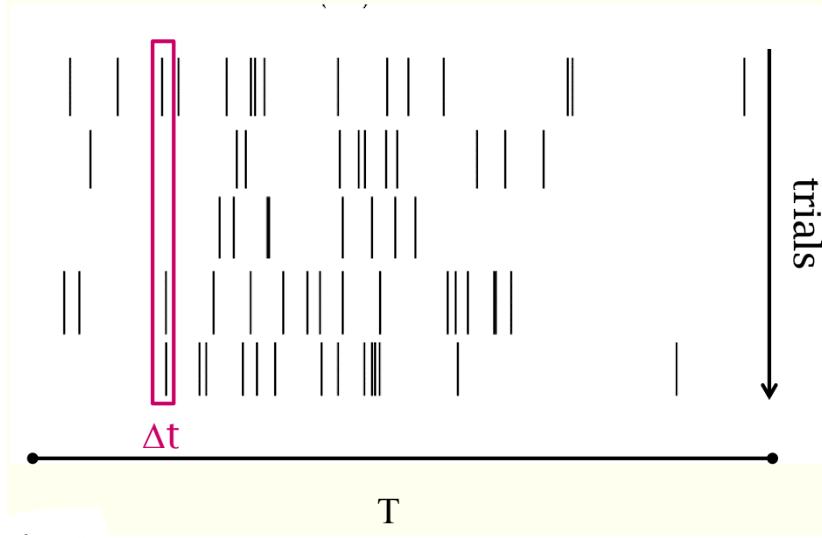
\includegraphics[width=0.4\textwidth]{images/spikes.png}
\end{figure}
The \textbf{Poisson Spike Generator} is a stochastic model of the neural response to a stimulus property $s$, it produces a spike trains with the same firing rate $r$ of the neural response:\begin{enumerate}
     \item We estimate the firing rate $r_{est}$ with experiments, and approximate the tuning curve $f$. 
     \item We build the spike generator based on a Poisson distribution with $r=r_{est}$.
\end{enumerate} 
The generator will produce a spike train that seems irregular and random, exactly like the activity of many real neurons. The following algorithm simulates the statistical results of the membrane:\bigskip

\noindent\textbf{Hypothesis}: The probability to generate a spike during the time interval $\Delta t$ is $r_{est}\Delta t$.
\begin{enumerate}
     \item We discretize the time in small intervals $\Delta t$. 
     \item At each time step, a random number $x_{rand}\in [0,1]$ is generated, with uniform probability. 
     \item For each time step $\Delta t$, if $r_{est}\Delta t>x_{rand}$, a spike is fired, otherwise not.
\end{enumerate}
By running this algorithm in a time interval $[0,T]$ divided in small step each of lenght $\Delta t$, we generate a spike train similiar to the original one measured by the sensors. We recall that $r_{est}$ depends on the stimulus property $s$ according to the experiments done.\bigskip 

This simulator is easy to setup but have an issue, in the real cell, having to consecutive spikes is impossible due to the refractory period of the ion channels, the generator does not take into account this phenomena, so it produces results slightly different from the real data:\begin{quotation}
     In the actual neuron the minimum inter spike distance is constrained, in the Poisson spike generator not.
\end{quotation}
We can build a more complex generator that includes such constraint.
\begin{figure}[H]
          \centering
          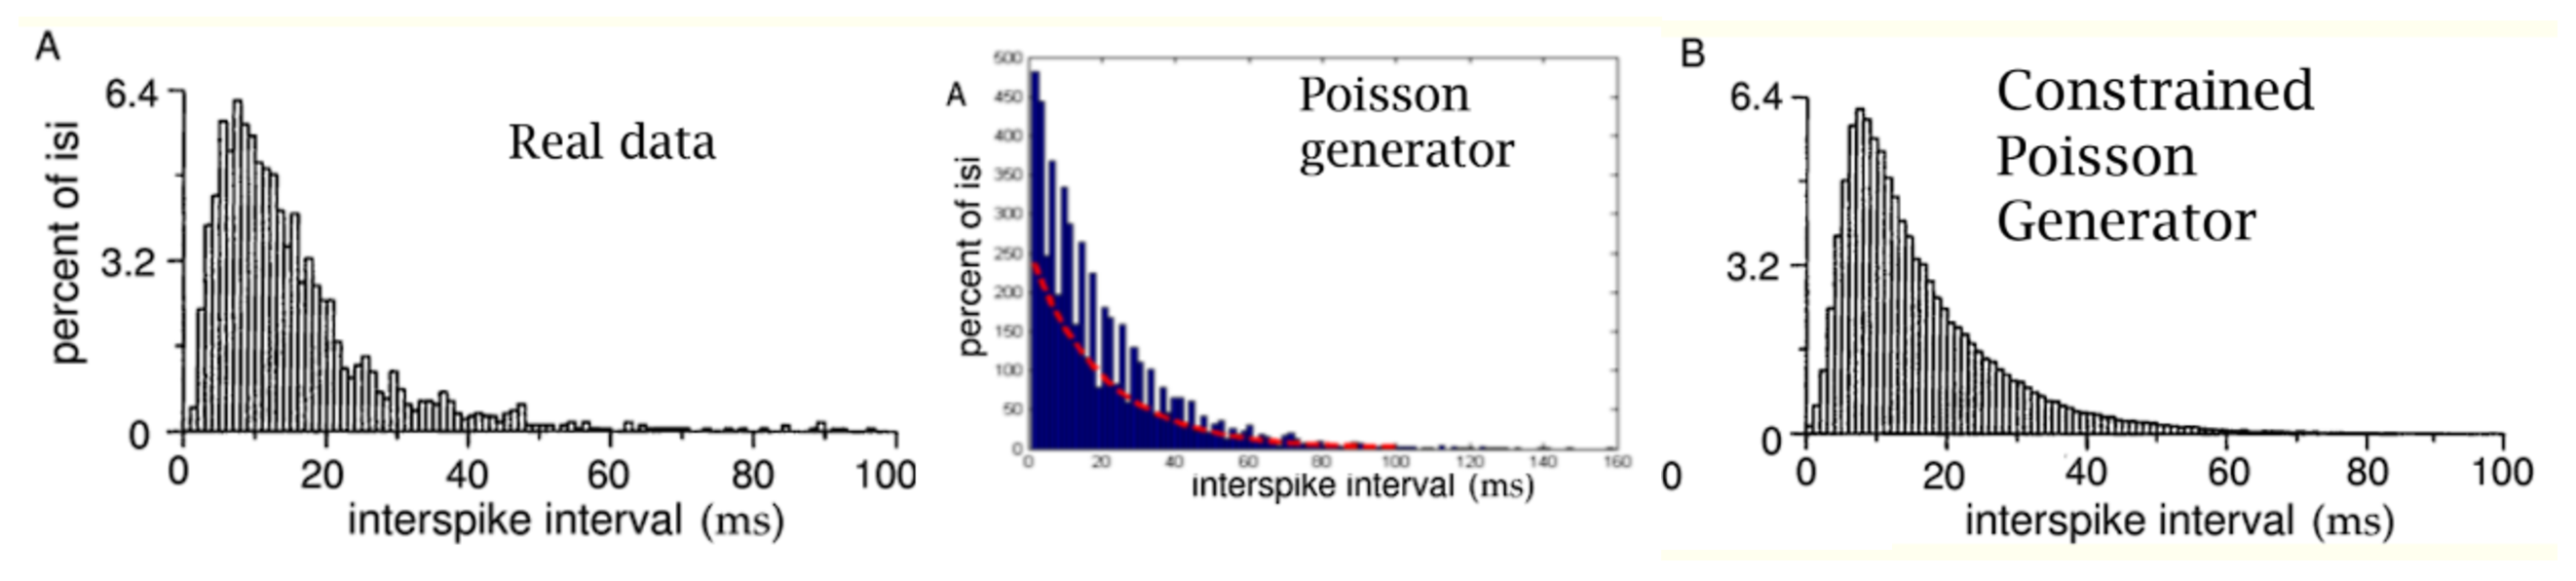
\includegraphics[width=\textwidth]{images/p_isi.eps}
          \caption{isi: Inter Spike Interval. }
\end{figure}
\section{Neural Decoding}
The input (stimulus) of the brain can be either external or internal, the output is a series of spike, with \textbf{neural decoding} we want to go back from the effect to the cause.
\begin{figure}[H]
          \centering
          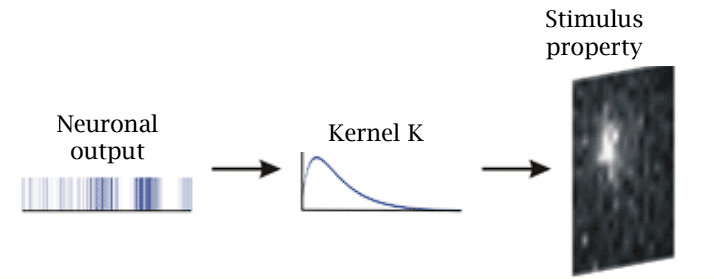
\includegraphics[width=0.5\textwidth]{images/decoding.png}
\end{figure}
Our goal is to compute the probability $\Prob(s|r)$ that a given stimulus $s$ produced the firing rate $r$. To explain the decoding process, we will use for the rest of the discussion the following case study: We have a human subject trained to recognize the \textit{motion direction} of dots on a screen. At each trial, the subject have to guess if the dots are moving upwards ($+$) or downward ($-$), in addition of that, there are a set of dots that moves randomly (neither upward or downward) and represents ''noise'' in the experiments. We call \textbf{coherence} the percentage of dots that moves  up (or downward), when the coherence is 0\%, all points moves randomly, when is 100\%, all dots moves together upward (or downward).\begin{figure}[H]
          \centering
          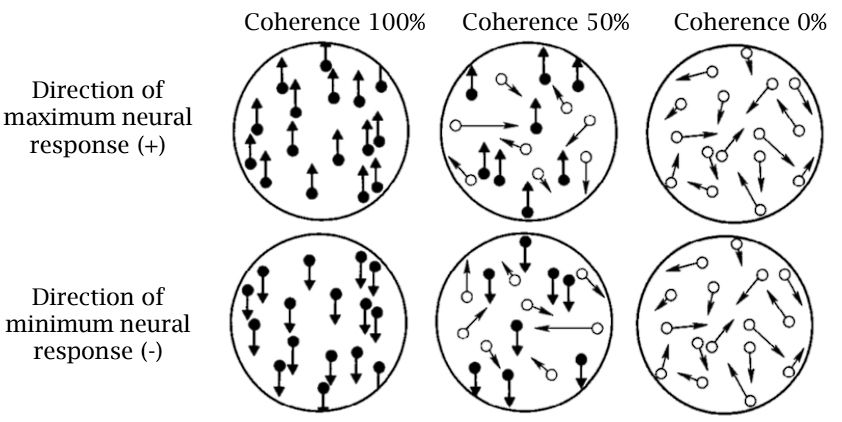
\includegraphics[width=0.6\textwidth]{images/dots.png}
\end{figure}
We observe in the behavioral data that the percentage of correct answer by a subject heavily depends on the coherence: If the coherence is 100\%, the percentage of correct answer is 100\%: the subject always discriminate the correct direction. When the coherence is 0\%, the subject guess the correct direction only in half of the trials. The ratio between correct answer and coherence is not linear:\begin{figure}[H]
          \centering
          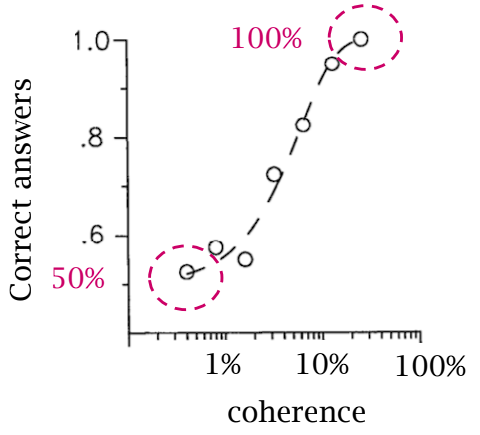
\includegraphics[width=0.3\textwidth]{images/coherence.png}
\end{figure}
With 90\% of dots that moves randomly, the subject is still able to correct identify more than 80\% of the trial: our brain recognize movement even in presence of noise. \bigskip 

The \textbf{goal of our neural decoder} is to guess if the dots were moving upward or downward \textbf{by observing the neural response} from the behavioral data.
Observe the hystogram in figure \ref{his_dot}, that have been constructed from behavioral data after 60 trials for each combination of the two factors (direction and coherence).
\begin{figure}
          \centering
          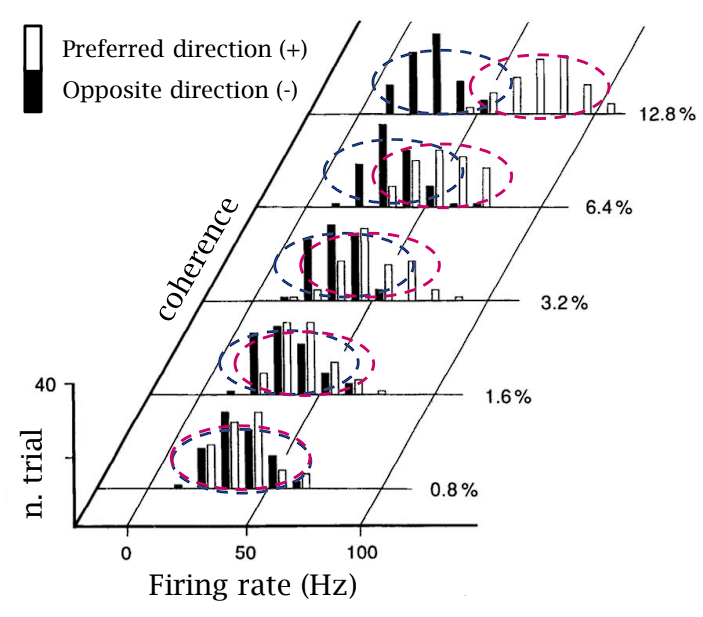
\includegraphics[width=0.6\textwidth]{images/histoDots.png}
          \caption{Dots experiment hystogram.}
          \label{his_dot}
\end{figure}
When the coherence rise, from 0\% to 12.8\%, the stimulus becomes more clear, the white curve shows how the neurons increase the firing rate while increasing the strength of the stimulus (from noise to precise direction).\begin{itemize}
     \item When the coherence is low, the two curves (representing the different directions) overlaps, the neuron behaves exactly the same.
     \item When the coherence increase the neurons start to show a difference in the response, in particularly, when the direction is $(+)$, the firing rate increases: The cells are able to respond to the upward direction and the distribution shift to the right. 
\end{itemize}
The hystogram shows that the response of the neurons when the dots moves downward is identical to the response when the dots moves randomly, instead when the dots moves upward, the firing rate of the neurons increases respect to the random noise. The two curves are both Gaussians with the same variance $\sigma_r^2$ but different means $\langle r\rangle_+$ and $\langle r\rangle_-$. The hystogram shows how $\langle r\rangle_-$ doesn't depend on the coherence, while $\langle r\rangle_+$ yes.\bigskip 

We define the \textbf{Discriminability}  $d'$ as follows\begin{equation}
     d'=\frac{\langle r\rangle_+-\langle r\rangle_-}{\sigma_r}
\end{equation}
and is the capacity of distinguish between different stimuli, when the coherence increase, $\langle r\rangle_+$ increase, and so also the discriminability becomes larger, $d'$ is a measure of the quality of the neuronal signal. \bigskip

In the hystogram, when the coherence is law, there is an overlap between the neuronal response when the direction is upward or downward. In this case, our decoder can't easily guess what was the preferred direction. Our neural decoder uses a threshold $z$ (decided by the designer) to guess the direction:\begin{itemize}
     \item Let $r$ to be the observed firing rate.
     \item If  $r\ge z$, the inferred direction is $+$.
     \item If  $r< z$, the inferred direction is $-$.
\end{itemize}
When the coherence is low and there is overlap, the decoder will makes more mistake.
\begin{figure}[H]
          \centering
          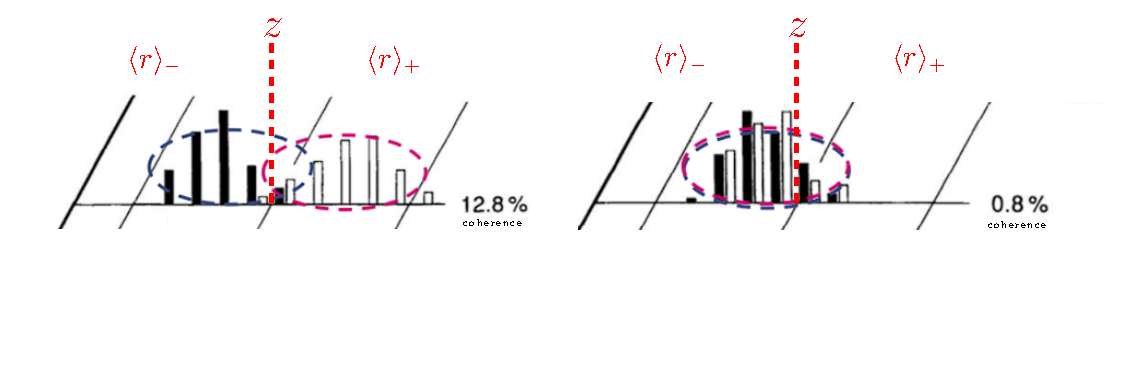
\includegraphics[width=\textwidth]{images/separator.eps}
          \caption{When the coherence is 12.8\%, the given threshold $z$ correctly separates the two classes of stimuli. Instead, when the coherence is 0.8\%, the threshold misclassify the majority of trials with $(+)$ direction.}
\end{figure}
\begin{itemize}
     \item true positive: The trial involved \textit{upward direction} and the threshold $z$ classified \textit{correctly} the trial.
     \item false positive: The trial involved \textit{downward direction} and the threshold $z$ classified \textit{wrongly} the trial.
     \item false negative: The trial involved \textit{upward direction} and the threshold $z$ classified \textit{wrongly} the trial.
     \item true positive: The trial involved \textit{downward direction} and the threshold $z$ classified \textit{correctly} the trial.
\end{itemize}
We denote $\beta(z)=\Prob(r\ge z|+)$ the probability of classifying a trial correctly, when the trial involved upward direction (the probability of guessing true positives), while $\alpha(z)=\Prob(r\ge z|-)$ is the probability of classifying a trial wrongly, when the trial involved downward direction (the probability of guessing true negatives). 

Ideally we would like $\beta(z)=1$ and $\alpha(z)=0$, we have to tune $z$ in order to reach this result.
\begin{table}[H]
     \centering
\begin{tabular}{|c|cc|}
\hline
\multirow{2}{*}{probability} & \multicolumn{2}{c|}{stimulus}                     \\ \cline{2-3} 
                             & \multicolumn{1}{c|}{+}            & -             \\ \hline
$r\ge z$                     & \multicolumn{1}{c|}{$\beta(z)$}   & $\alpha(z)$   \\ \hline
$r<z$                        & \multicolumn{1}{c|}{$1-\beta(z)$} & $1-\alpha(z)$ \\ \hline
\end{tabular}
\end{table}
A nice way to plot the performance of the decoder, with a given threshold $z$ is through the \textbf{Receiver Operating Characteristic (ROC) curves}: We consider a plane where the $x$-axis represents the value of $\alpha(z)$ and the $y$-axis the value of $\beta(z)$, both going from 0 to 1, given a choice for $z$, we plot on the plane the point relative to that choice, for example:
\begin{figure}[H]
          \centering
          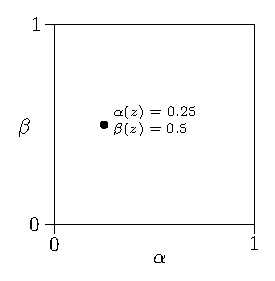
\includegraphics[width=0.3\textwidth]{images/ROC1.eps}
\end{figure}
We let $z$ to change for 0 toa certain frequency, and plot different ROC curves for different values of coherence:
\begin{figure}[H]
          \centering
          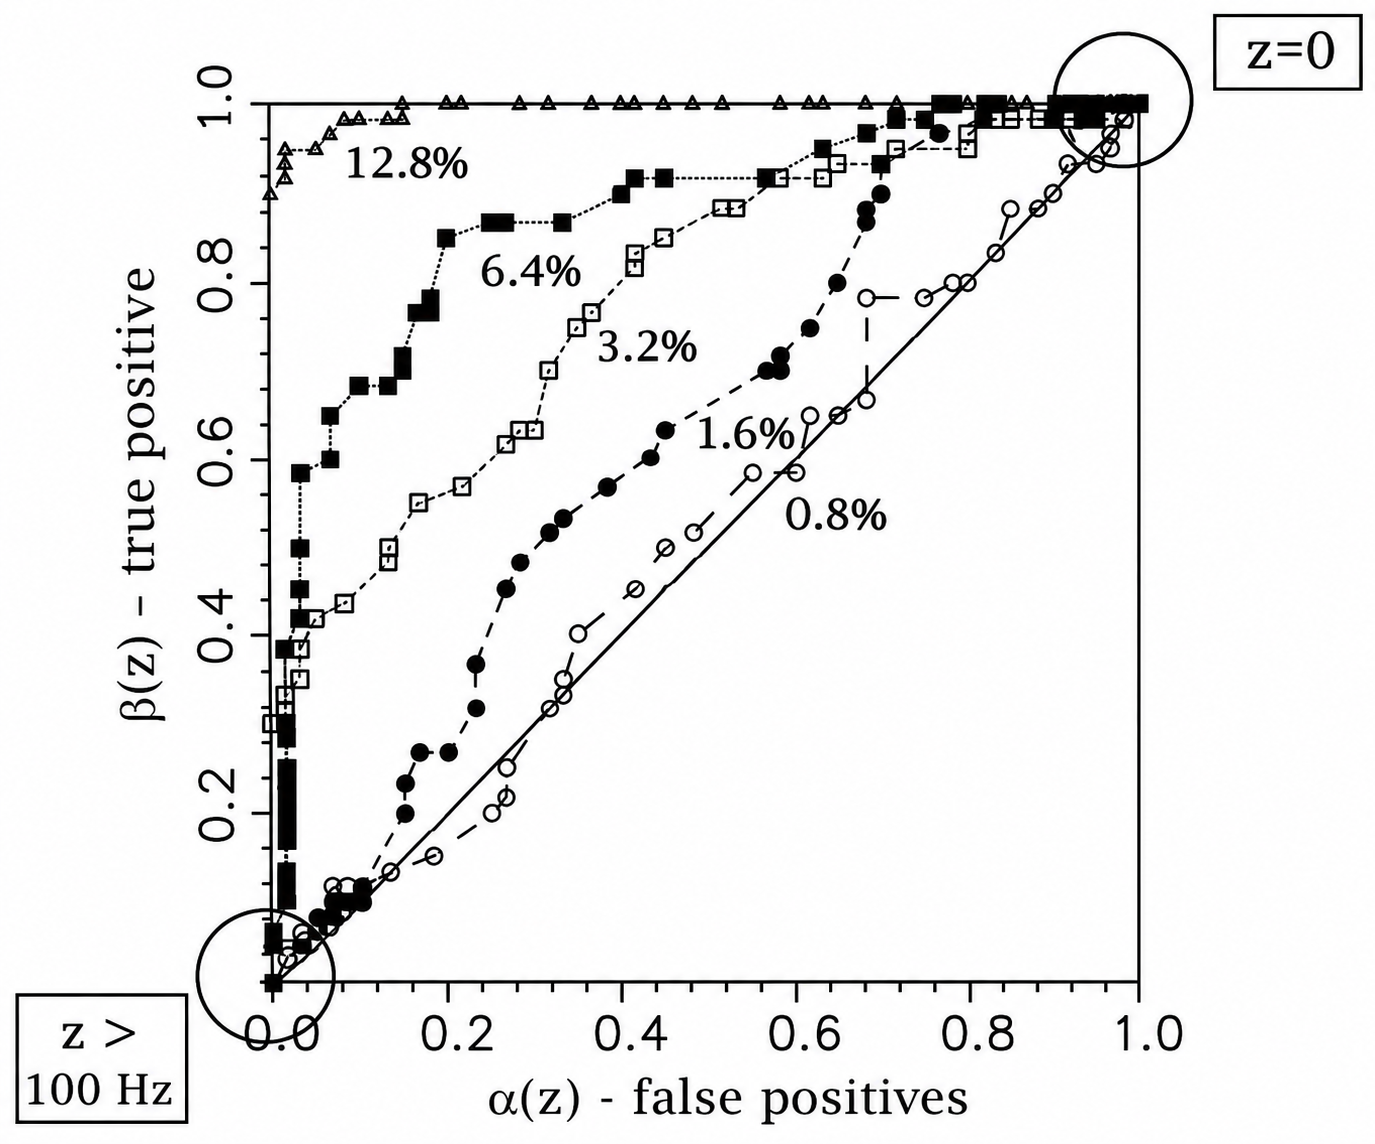
\includegraphics[width=0.5\textwidth]{images/ROC2.png}
\end{figure}
All the curves shares the same starting and ending point, of course the best value of $z$ is the one relative to the point nearest to $(0,1)$.

When the coherence is near to 0\%, the curve is near the line $\alpha=\beta$, in this case choosing different values of $z$ does not increase performance and the points remain close to this line. The increasing coherence makes the ROC curves to be ''attracted'' by the point $(0,1)$. Given a certain curve, the best choice of $z$ can be derived just by looking at the point nearest to the top left corner.
\begin{figure}[H]
          \centering
          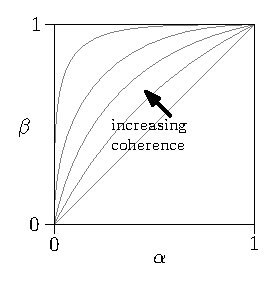
\includegraphics[width=0.25\textwidth]{images/ROC3.eps}
\end{figure}
The performances of a classifier are evaluated by the area under the ROC curve (AUC), and represents the percentage of correct classifications. Of course the best possible value for the AUC is 1, and the worst possible value is the area under the curve $\alpha=\beta$ that is $\nicefrac{1}{2}$: That is also the result of trying to guess randomly.
\bigskip

This classifier is not sophisticated, but performs similar to the behavioral data fetched from the human experiments. The neural decoding task is involved, we need to study how the brain works in a probabilistic fashion, we need to understand how the neurons works and build distributions, in order to develop a strategy to decode the information. An accurate decoder would require complex computation, a conflicting requirement with respect to the bit rate (how fast we can decode the data), so in real applications there is a trade of between these two requirements.
\chapter{Brain Networks}
To extract useful information from biological signals such as EEG, we must decide with which ''lens'' to observe these signals. The fundamental distinction in neuroengineering is that between univariate and multivariate approaches.\begin{itemize}
     \item \textbf{Univariate Analysis}: We treat each signal as a single entity, we calculate statistics, averages or variations on that signal without worrying about what the other signals are doing at the same time.
     \item \textbf{Multivariate Analysis}: The human brain is a complex system with communicating parts. Multivariate analysis doesn't just look at the signals, but looks for the relationships, correlations and interdependencies between them.
\end{itemize}
\section{Network Neuroscience}
In \textbf{Network Neuroscience} the nervous system is seen as a complex network, this discipline aims to map, record, analyze and model the elements and interactions between neurobiological systems.

The objective is to estimate \textit{dynamic brain networks} at all levels  (among molecules, neurons, brain areas and social systems). In this discipline there is the intersection of two fundamental approaches:\begin{itemize}
     \item Empirical Approach: It is based on the collection of real data (neuroimaging, electrophysiology, microscopy).
     \item Computational Approach: It is based on mathematical modeling. Once we have the data, we use algorithms and simulations to predict how the system will behave in the future or how it will react to an injury or stimulus.
\end{itemize}

The functionally specialized regions of neurons are physically connected between them, through the axons, and interact within and between themselves, forming brain networks.
\begin{figure}[H]
          \centering
          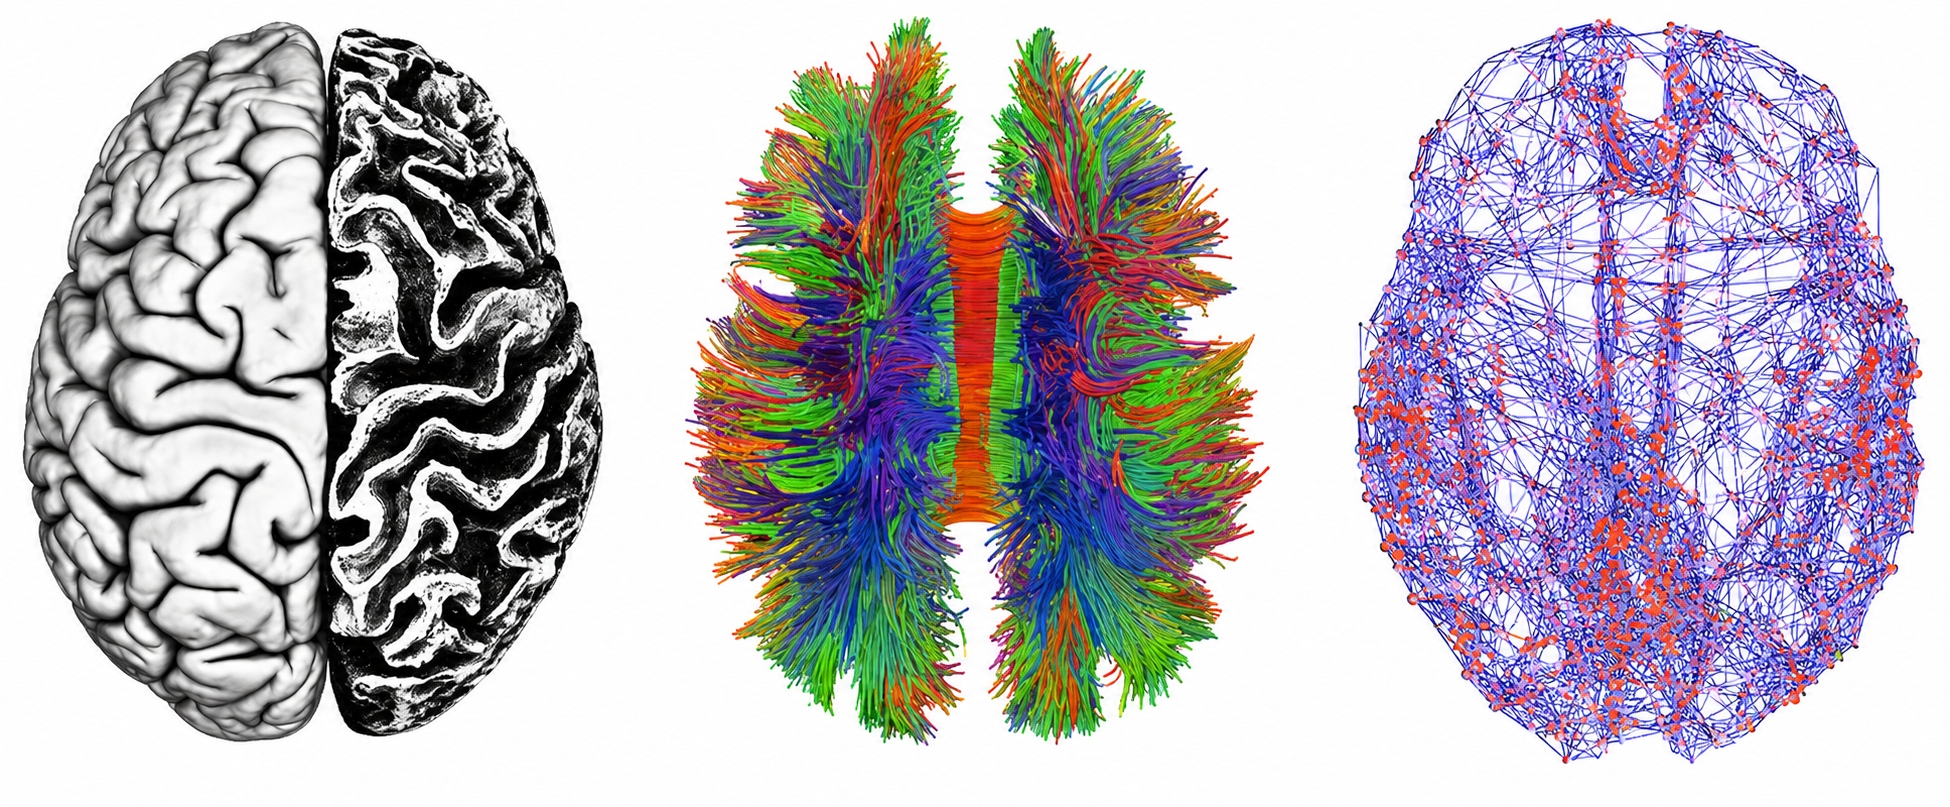
\includegraphics[width=0.6\textwidth]{images/brain_network.png}
\end{figure}
To correctly model the brain, we need two types of information, represented by the two incoming flows to the modeling center:\begin{itemize}
     \item \textbf{Brain Activity}: It is the dynamic component. It tells us what is happening in the brain at any given moment (e.g. voltage fluctuations, changes in blood flow).
     \item \textbf{Brain Connectivity}:  It is the structural and organizational component. It is the map of interactions. As you can see in the diagram, this is divided into \textit{three levels} of increasing complexity.
\end{itemize}
\subsection{Anatomical, Functional and Causal Connectivity}
The \textbf{three levels} of brain connectivity are:\begin{enumerate}
     \item Anatomical: It represents the white matter tracts, the axons that physically connect two brain areas. It is the static structure.
     \item Functional: Represents a statistical dependency. If area $A$ and area $B$ show signals that vary together over time (correlation), we say they are ''functionally connected''.
     \item Causal: It's the highest level. Here we model the directionality of influence. Does area $A$ have a causal influence on area $B$? It is the level necessary to understand the flow of information and control dynamics.
\end{enumerate}
The modeling of the brain have four main domains of applications: Understand the cognitive functions, understand how the brain evolves over time (plasticity), clinical applications and industrial applications.\bigskip

The \textbf{anatomical connectivity} is the physical layer (like the axons) that physically connects the brain areas, or single neurons between them. This structure is stable in the short time, and does not change. Can change only at a longer time scale (plasticity), as already described in Section \ref{Plasticity}. There are two ways to study this layer:\begin{itemize}
     \item Invasive (Tracing): Chemical tracers are used that are injected into neurons and ''go up'' or ''down'' along the axons to map the connections. It is very precise, but obviously it can only be done in pre-clinical studies (on animal models).
     \item Non Invasive (Diffusion Weighted Imaging): A result of this technique is shown in figure \ref{DTI}. It exploits the way water molecules move within axons. Since water tends to diffuse along the direction of the nerve fibers, the computer can reconstruct the path of the fiber bundles. It is the technique that allows us to ''see'' the wiring of the human brain in vivo.
\end{itemize}
\begin{figure}[H]
          \centering
          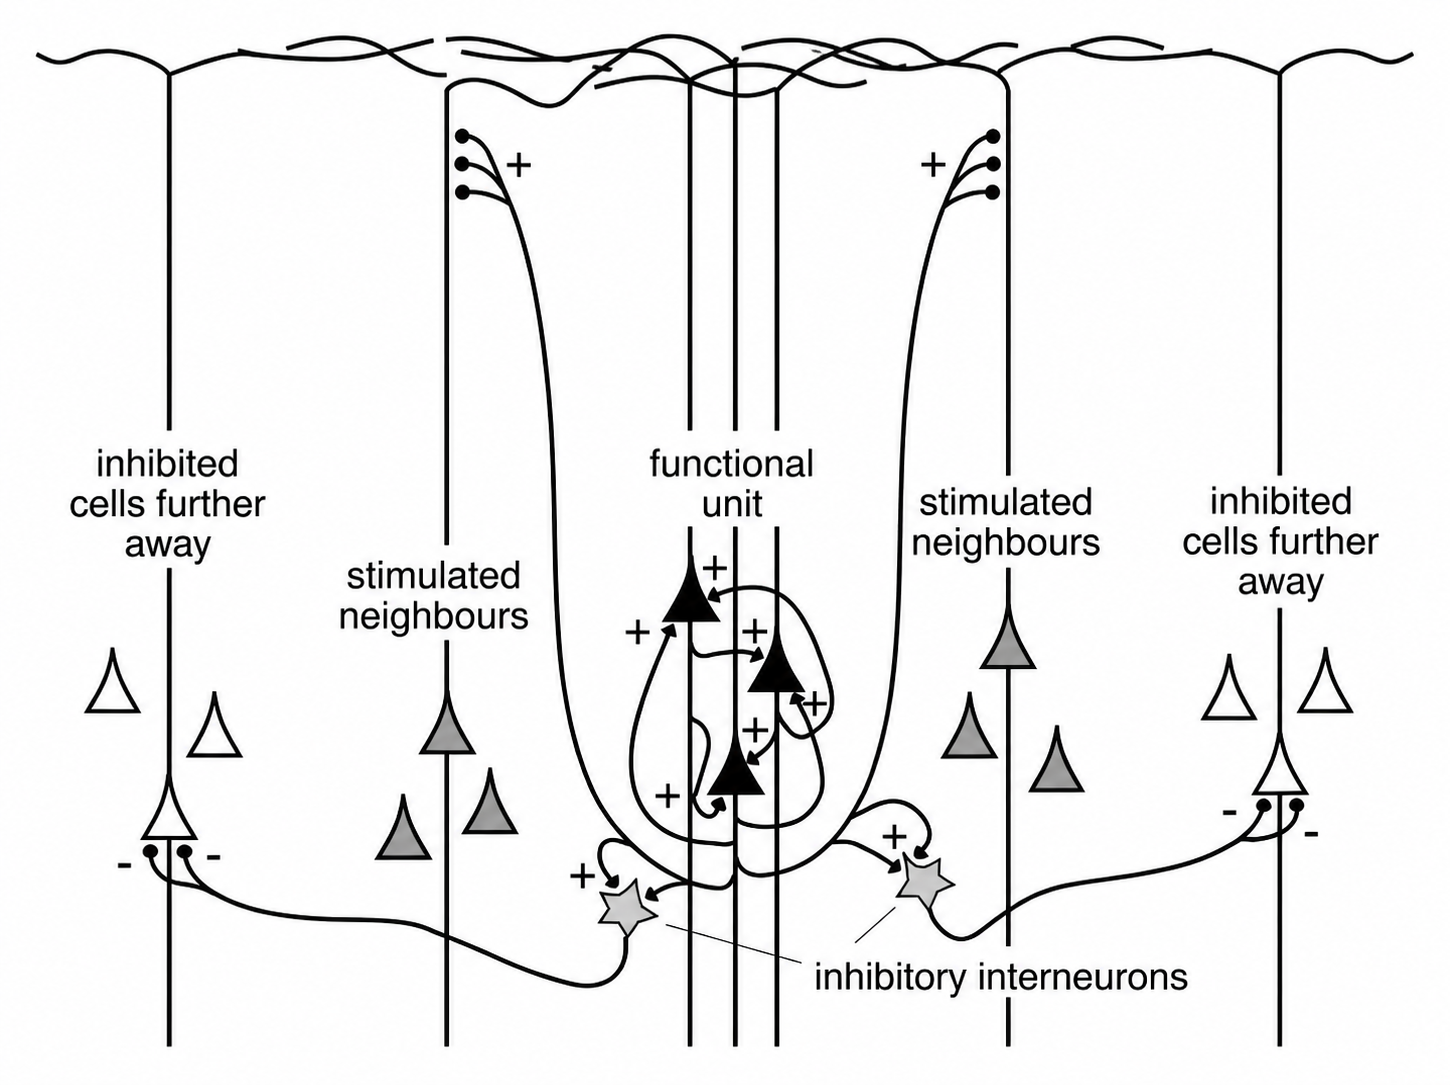
\includegraphics[width=0.4\textwidth]{images/anatomicalConn.png}
\end{figure}
Anatomical connectivity is at the basis of 
functional/effective connectivity, but cannot 
explain it.\bigskip

While with anatomical connectivity we try to understand how the brain is built, with \textbf{functional connectivity} we try to understand how it is working at a given moment. The key distinction here is that, unlike other methods, functional connectivity is a purely statistical measure. At this level the principle of non-causality applies: if two brain areas ($A$ and $B$) show synchronized activity (e.g. their electrical signals rise and fall together), functional connectivity simply records this fact. It does not assume that $A$ is controlling $B$, nor that $B$ is controlling $A$. Being ''essentially descriptive'', this technique does not attempt to explain the biological mechanism behind the connection. It simply describes the state of the system through mathematical measurements. We quantify this synchrony trough:\begin{itemize}
     \item Correlation: Calculates how linear the fluctuations of two signals are to each other.
     \item Coherence: Measures the synchrony between two signals in the frequency domain.
     \item Transfer Entropy: A more advanced measure that seeks to quantify how much the uncertainty about one signal is reduced by knowing the history of the other.
\end{itemize}

The highest level is the \textbf{causal connectivity}. Effective connectivity describes the direct and directional influence that one brain area has on another. We are no longer satisfied with saying ''$A$ and $B$ are active together''; we want to prove that ''$A$'s activity is causing a change in $B$'s activity''.
Causal connectivity is guided by models, we need a model that describes how the area $A$ interacts with the area $B$, and then test this model with respect to the real data. In this approach we need an hypothesis \textbf{at priori} of how the system might work: We try different models from a wide model space, and check which model performs better (sticks better to the real data).
\begin{figure}[H]
          \centering
          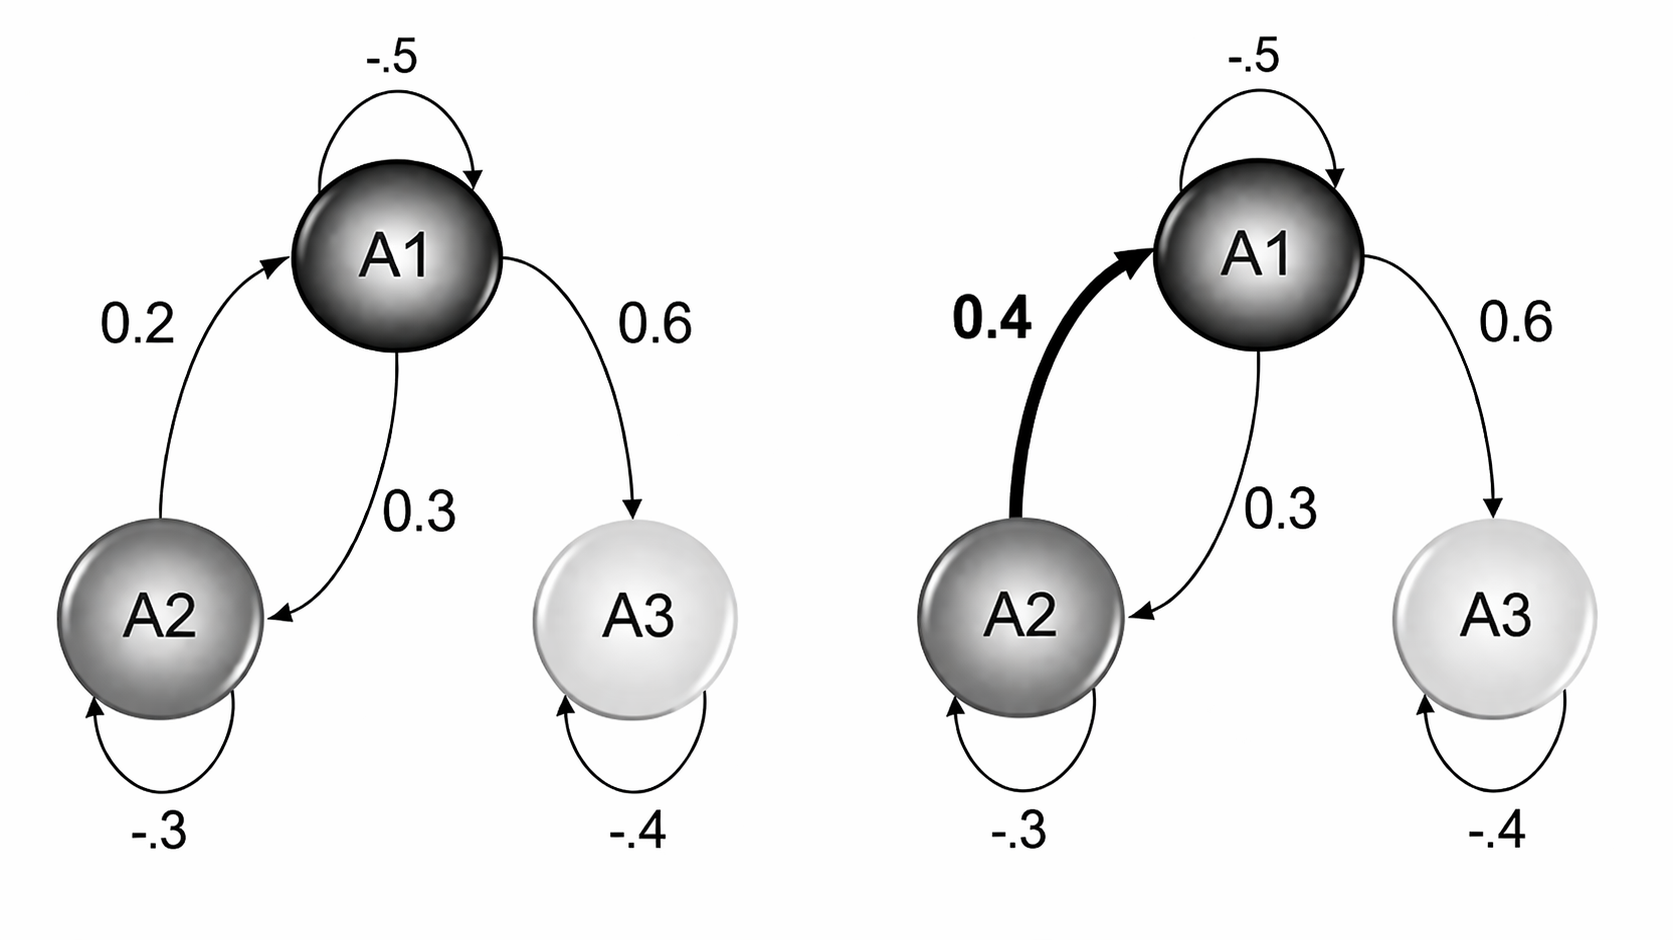
\includegraphics[width=0.5\textwidth]{images/causality_graph.png}
          \caption{Causality graph.}
          \label{causality_graph}
\end{figure}
\noindent A simple model of causality is shown in figure \ref{causality_graph}. The nodes A1, A2 and A3 represents units of the system (populations of neurons or specific brain areas). If there is an edge from A2 to A1, it means: \textit{the activity of the population A2 causes a change in the activity of A1}. It's not a simple correlation; it is a dynamic impact hypothesis.

The numbers on the edges represents weights or coupling parameters, they represent the ''strength'' of the influence. The two different graphs represents two different models (hypothesis). A comparison with the data will determine which of the two models better describes the brain. 
\subsection{Correlation and Coherence}
The \textbf{Hebbian Theory}  states that:\begin{quote}
     ''Cells that fire together wire together''.
\end{quote}
Hence, region correlation (physical) can be associated to synchronization (and viceversa). The brain organize information on multiple dimensions, one of them is the following:\begin{itemize}
     \item \textbf{Spectral}: The brain oscillates at different frequencies. Low frequencies (e.g. Delta, Theta) tend to coordinate distant areas and are involved in global integration processes or in sleep. High frequencies (e.g. gamma) are typical of local, fast and computationally intensive processes.
\end{itemize}
Due to their excellent temporal resolution, neuroelectrical measures (from invasive to scalp recorded EEG) keep the information coded in the brain rhythms.
\begin{figure}[H]
          \centering
          \includegraphics[width=0.5\textwidth]{images/spectral.png}
\end{figure}
In this section we provide mathematical procedure to describe the correlation and coherence between two signals. For example, a trace of the EEG is stored as a discrete time signal: A time series $x[n]$ with sampling interval $T$.
\begin{figure}[H]
          \centering
          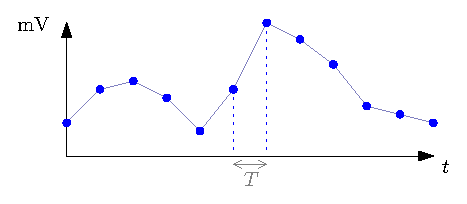
\includegraphics[width=0.4\textwidth]{images/eegTrace.eps}
\end{figure}
We need two definitions.
\begin{boxdefinition}{Auto Correlation Function}{}
     Given a time series $x[n]$, the auto correlation function is the time series:\begin{eqnarray}
          r_{xx}[k]=\sum_{n=-\infty}^{+\infty}x^*[n]x[n+k].
     \end{eqnarray}
\end{boxdefinition}
\begin{boxdefinition}{Cross Correlation Function}{}
      Given two time series $x[n]$ and $y[n]$, the cross correlation function is the time series:\begin{eqnarray}
          r_{xy}[k]=\sum_{n=-\infty}^{+\infty}x^*[n]y[n+k].
     \end{eqnarray}
\end{boxdefinition}
With $x^*[n]$ we denoted the complex conjugate of $x[n]$, for real signals like the EEG (that is measured in mV), the immaginary part is null, hence the complex conjugate is identical to the original sample. In the mathematical definitions the signals are defined from $t=-\infty$ to $t=+\infty$, of course the real signals are defined only in a limited time window.\bigskip 

The auto correlation function describes the internal structure of the signal, while the cross correlation describe the interaction between two signals, the latter requires (obviously) tha the two signals are recorded simultaneously.
\begin{boxdefinition}{Fourier Transform}{}
     The Fourier transform of a time series $x[n]$ with sampling interval $T$ is the continuous function:\begin{equation}
          X(f)=\sum_{n=-\infty}^{+\infty}x[n]\exp(-j2\pi fnT).
     \end{equation}
\end{boxdefinition}
This definition is also given in the Chapter \ref{sig_proc}. As we know, it describes the signal in the frequency domain. We denoted $j$ the imaginary unit.
\begin{boxdefinition}{Power Spectral Density}{}
     The Power Spectral Density (PSD) of the time series $x[n]$ is the square amplitude of it's Fourier transform:\begin{equation}
          S_{xx}(f)=|X(f)|^2.
     \end{equation}
\end{boxdefinition}
The PSD is a fundamental measurement in signal analysis that indicates how the power (or energy) of a signal is distributed over frequency.
In practical terms, looking at a PSD graph allows you to immediately identify the dominant frequencies of a system. For example, if you analyze a signal, the PSD will show you high peaks at the frequencies where most of the activity is concentrated, while flatter areas indicate frequencies with less energy or simple background noise.
\begin{boxtheorem}{Wiener-Khinchin (auto correlation)}{}
     The PSD of a time series $x[n]$ can be computed by evaluating the Fourier transform of the auto correlation function of $x[n]$:\begin{equation}
          S_{xx}(f)=\sum_{n=-\infty}^{+\infty}r_{xx}[n]\exp(-j2\pi fnT).
     \end{equation}
\end{boxtheorem}
\noindent Another important quantity for two signals $x[n]$ and $y[n]$ is the \textbf{mutual PSD}.\begin{boxdefinition}{Mutual Power Spectral Density}{}
     The mutual PSD of two time series  $x[n]$ and $y[n]$ is the following real function:\begin{equation}
          S_{xy}(f)=X(f)Y^*(f)=Y(f)X^*(f)=S_{yx}(f).
     \end{equation}
\end{boxdefinition}
\noindent The mutual PSD tells how much power two signals share at each frequency.
\begin{boxtheorem}{Wiener-Khinchin (cross correlation)}{}
     The mutual PSD of two time series $x[n]$ and $y[n]$ can be computed by evaluating the Fourier transform of the cross correlation function:\begin{equation}
          S_{xy}(f)=\sum_{n=-\infty}^{+\infty}r_{xy}[n]\exp(-j2\pi fnT).
     \end{equation}
\end{boxtheorem}
\noindent Given two signal $x[n]$ and $y[n]$ we can define the symmetrical \textbf{spectral matrix}:\begin{equation}
     S(f)=\begin{pmatrix}
          S_{xx}(f)&S_{xy}(f)\\
          S_{yx}(f)&S_{yy}(f)
     \end{pmatrix}.
\end{equation}
So the relations of these two signals in the frequency domain is embedded in this matrix $S(f)$, for each frequency $f$.
As we already mentioned, with \textbf{coherence} measures the synchrony between two signals in the frequency domain.

\begin{boxdefinition}{Ordinary Coherence}{}
     The \textbf{Ordinary Coherence} $C_{xy}(f)$ is the \textit{linear correlation} between two signals at a given frequency:\begin{equation}
          C_{xy}(f)\frac{|S_{xy}|^2}{S_{xx}(f)S_{yy}(f)}.
     \end{equation}
\end{boxdefinition}


It's the Mutual Power Spectral Density divided by the 
product of their individual power spectral densities. The ordinary coherence is a spectral function (depends on the frequency $f$) and it's normalized between 0 and 1. For a given frequency $f'$:\begin{itemize}
     \item $C_{xy}(f')=0 \ \implies$ the two signals are \textbf{independent} at that frequency.
     \item $C_{xy}(f')=1 \ \implies$ the two signals are \textbf{maximally correlated} at that frequency. 
\end{itemize}
The ordinary coherence does not contain any information about the direction of the interaction, it measures only the synchronicity but not causality. this is a problem since a simple correlation between two events does not directly imply that one of these cause the other (and viceversa). For example, if the two events are the effects of a common source, these two will have an high correlation, although they have no causal relationship between them.

\subsection{Causality}

The determination of causal relationships in neural networks is mainly articulated through two distinct approaches. The first, defined \textit{Physical Influence} (or interventional approach), is based on direct experimental manipulation (e.g. via electrical stimulation or ultrasound) of a node in the network; this physical intervention isolates the influence of the manipulated node, allowing it's distal effects to be measured, representing the \textit{gold standard} for defining causality, although it is limited by constraints of experimental practicality. The second approach, based on \textit{Temporal Precedence}, is observational in nature and postulates that the cause must temporally precede the effect; in this context, causality is inferred via computational analyzes that evaluate the predictive ability of temporally distinct neural events, allowing directional influences to be derived from raw data without the need for invasive physical manipulations.\bigskip


The first definition of causality in a statistical framework was given by Norbert Wiener in 1956.\begin{boxdefinition}{Causality}{}
Given two simultaneously measured signals, if one can 
predict the first signal better by incorporating the past 
information from the second signal than using only 
information from the first one, then the second signal 
can be called \textbf{causal} to the first one.
\end{boxdefinition}
Granger introduced a new concept of causality, at it's core, his theory states that:\begin{quotation}
     ''Causality is a matter of prediction.''
\end{quotation} 
If the activity of a signal $x[n]$ helps you predict the future of signal $y[n]$ better than you can by looking only at the past history of $y[n]$, then $x$ \textbf{Granger-cause} $y$. In an informal way:\begin{itemize}
     \item i have the time series $x[n],y[n]$ for $0\le n\le T$. I want to predict $y[T+1]$
     \item i use $y[0]\dots y[T]$ to have a prediction $\hat y[T+1]$, having an error $e_y=|\hat y[T+1]-y[T+1]$|.
     \item i use $y[0]\dots y[T]$ and $x[0]\dots x[T]$ to have a prediction $\hat y'[T+1]$ (for now we do not specify how the signal $x$ should be used to predict $y$), having an error $e_{yx}=|\hat y'[T+1]-y[T+1]|$
     \item if $e_{yx}<e_y$, then $x$ \textbf{Granger-cause} $y$.
\end{itemize}
\begin{figure}[H]
          \centering
          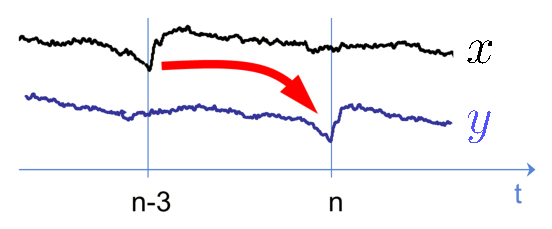
\includegraphics[width=0.7\textwidth]{images/grangerCause.eps}
\end{figure}
We have to define how to perform the prediction.
If we have to use only the past values of $x$ from 0 to $n-1$, the value of $x[n]$ can be predicted by the previous $p$ samples $x[n-1],x[n-2]\dots x[n-p]$ by a \textbf{Linear Autoregressive Model}:\begin{align}\label{lin_autore}
     &\hat x[n]=\sum_{k=1}^pa[k]x[n-k] \ + e[n]
     \\
     &=a[1]x[n-1]+a[2]x[n-2]+\dots +a[p]x[n-p]+e[n]
\end{align}
where $a[1]\dots, a[p]$ are real coefficients, and $$e[n]=x[n]-\hat x[n]$$ is the error between the prediction and the real value. $p$ is the \textbf{order} of the model (how many previous step we use to predict the future). We assume that the error $e[n]$ is a zero mean uncorrelated white noise.

To define a good model we have to determine the coefficients $a[k]$ that minimizes the squared error $e[n]$, this can be done by solving an optimization problem over experimental data.\bigskip 

Now, the Granger-causality is modeled through a \textbf{Bivariate Autoregressive Model}, let $x$ to be the signal that we want to predict, we have also another signal $y$. We want to use $x[0]\dots, x[n-1]$ and $y[0]\dots, y[n-1]$ to predict $x[n]$, the bivariate autoregressive model (of order $p$) for the prediction $\hat x[n]$ is defined as follows:\begin{equation}\label{biv_autore}
     \hat x[n]=\sum_{k=1}^p a_{xy}[k]x[n-k] 
     +\sum_{k=1}^p b_{xy}[k]y[n-k]  \ +e_{xy}[n].
\end{equation}
The regressive model to predict $y[n]$ using $x$ and $y$ is defined in a similar way as follows:
\begin{equation}
     \hat y[n]=\sum_{k=1}^p a_{yx}[k]y[n-k] 
     +\sum_{k=1}^p b_{yx}[k]x[n-k]  \ +e_{yx}[n].
\end{equation}
If we use experimental data to define two models to predict $x[n]$, one using just $x$ (linear autoregressive) as defined in equation \eqref{lin_autore}, and the other using both $y$ and $x$ (bivariate autoregressive) as defined in equation \eqref{biv_autore}, and we observe that $e_{xy}[n]<e[n]$, then we know that $y$ Granger-cause $x$.
\begin{figure}[H]
          \centering
          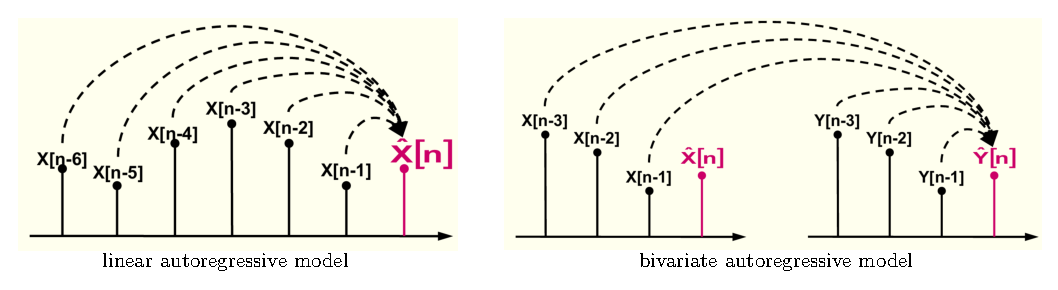
\includegraphics[width=0.9\textwidth]{images/predictions.eps}
\end{figure}
\noindent\textbf{Causality Test}: The prediction performances for both models can be assessed by the \textit{variances} of the prediction errors:$$\begin{matrix}
     V_{x|x}=\text{var}(e_x)& &  V_{x|x,y}=\text{var}(e_{xy})\\
     V_{y|y}=\text{var}(e_y)& &  V_{y|y,x}=\text{var}(e_{yx})
\end{matrix}$$
$x|x$ indicate predicting $x$ by its past values alone and $x|x,y$ indicate predicting $x$ bt its past values and the past values of $y$. If $V_{x|x,y}<V_{x|x}$ then $y$ Granger-cause $x$ in the sense of Granger causality, and a measure of this causality is given by:\begin{equation}
     G_{y\rightarrow x}=\ln\left(
          \frac{V_{x|x}}{V_{x|x,y}}
     \right)
\end{equation}
that measures ''how much'' $y$ cause $x$. To measure how $x$ cause $y$ we have:\begin{equation}
     G_{x\rightarrow y}=\ln\left(
          \frac{V_{y|y}}{V_{y|y,x}}
     \right).
\end{equation}
If the past of $y$ does not improve the prediction of $x$, then $V_{x|x,y}\simeq V_{x|x}\implies G_{y\rightarrow x}\simeq 0$. Any improvement in prediction of $x$ by the inclusion of $y$ makes $V_{x|x,y}$ decrease, and consequently $G_{y\rightarrow x}$ increase. Any addition of information should never decrease the model accuracy: $V_{x|x,y}$  should not be greater than $V_{x|x}$ (if it does, there's probably something wrong with the modelling):\begin{equation}
     G_{y\rightarrow x}\in [0,+\infty].
\end{equation}
\textbf{Advantages}:\begin{itemize}
     \item Directionality: $G_{y\rightarrow x}\ne  G_{x\rightarrow y}$. 
     \item Statistical meaning.
\end{itemize}
\textbf{Limitations}:\begin{itemize}
     \item Defined in the time domain (in the time window we used to
identify the model) provided that the signals are stationary in
that window.
     \item True causality can only be assessed if the set of two time series
contains all possible relevant information and sources of
activities for the problem.
\end{itemize}
\section{Pairwise and Multivariate Approaches}
Let's consider a set of signals that we have sampled from a process:\begin{equation}
     x_1[n], \ x_2[n] \ \dots \ x_i[n] \ \dots \ x_N[n]
\end{equation}
We might analyze all these signals pairwise and assess causality between each couple. The problem is that any pairwise model analyzing the relation between two signals cannot recognize the statistical link between them is due
to the common effect of a third signal,
which is not included in the model.\begin{center}
     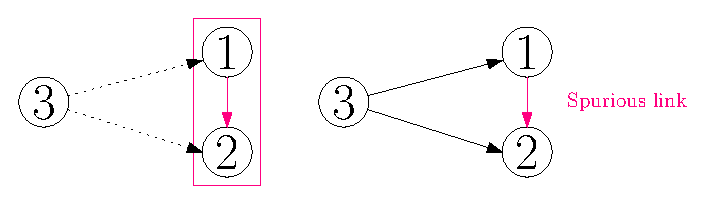
\includegraphics[width=0.6\textwidth]{images/Spurious_link.eps} 
\end{center} 
An \textbf{example} of this concept is the following: In summer the whether is hot, this means that ice cream shops sell more ice creams and that at three in the afternoon there are fewer people around: These two effects are related as they come from the same cause (the heat), despite this, they are not directly caused by each other.
\begin{figure}[H]
     \centering
     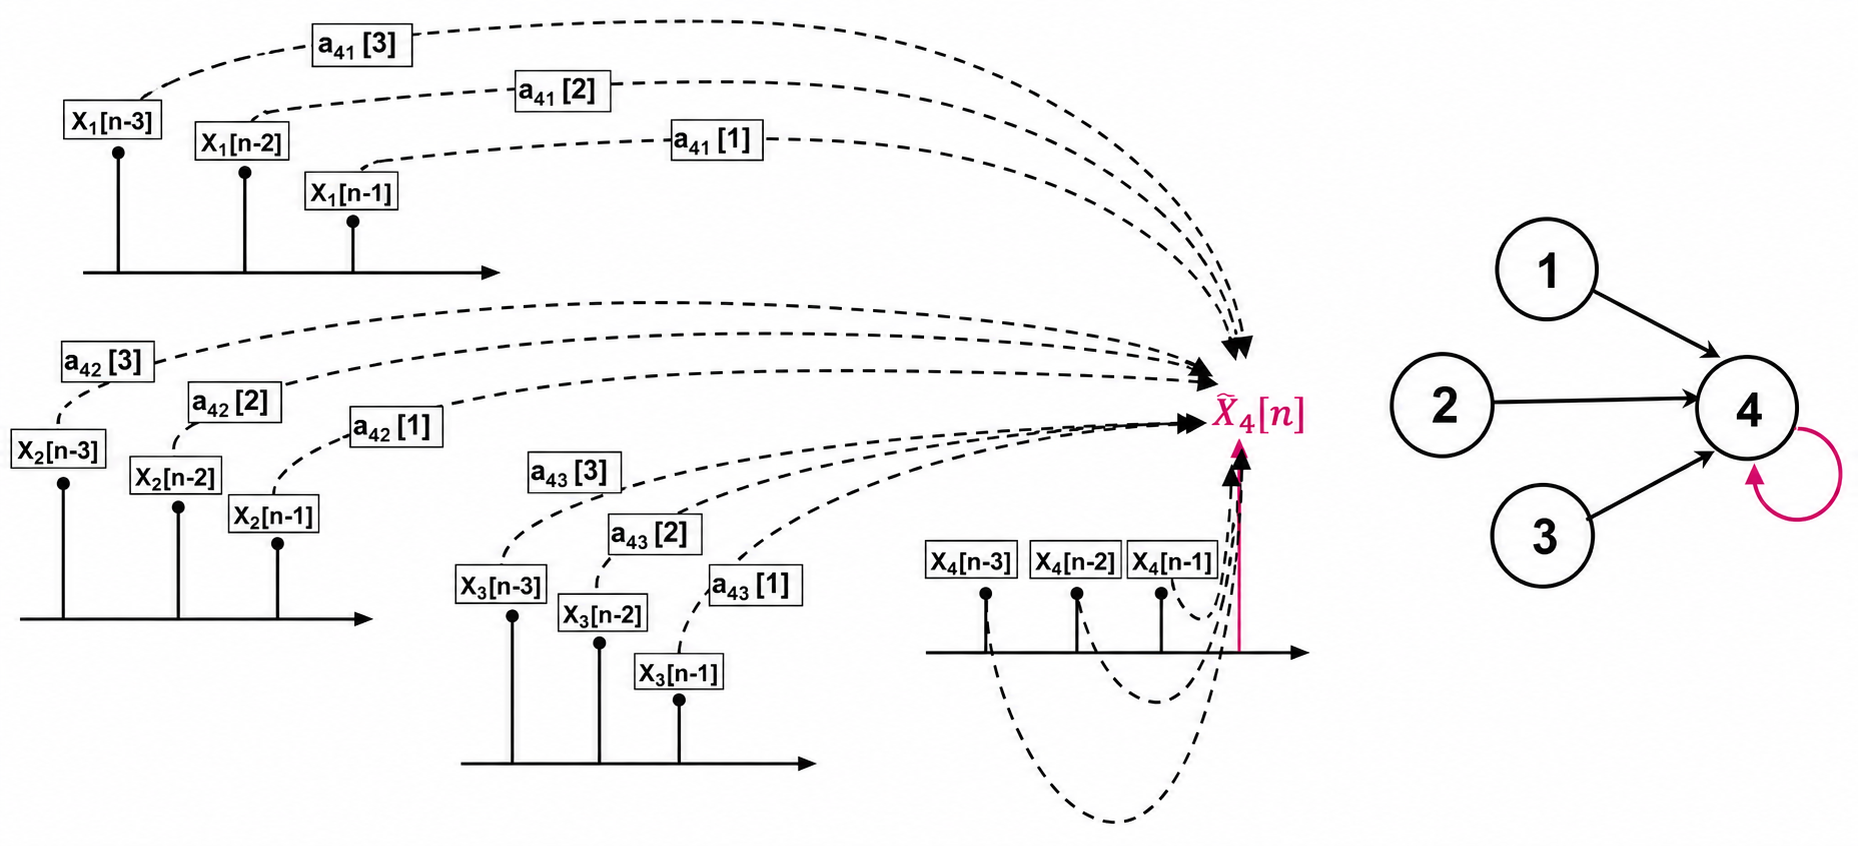
\includegraphics[width=0.8\textwidth]{images/MVAR.png}
\end{figure} 
In a \textbf{Multivariate autoregressive model (MVAR)}, the prediction of each signal $x_i$ is take by considering all the available $N$ signals, the mathematical regressor (that analyze the past $p$ observations) is defined as follows:\begin{align}
     & x_1[n]=-\sum_{k=1}^pa_{11}[k]x_1[n-k]-\sum_{k=1}^pa_{12}[k]x_2[n-k]-\dots -\sum_{k=1}^pa_{1N}[k]x_N[n-k]+e_1[n]\\ 
     & x_2[n]=-\sum_{k=1}^pa_{21}[k]x_1[n-k]-\sum_{k=1}^pa_{22}[k]x_2[n-k]-\dots -\sum_{k=1}^pa_{2N}[k]x_N[n-k]+e_2[n]\\ &\vdots \\
     & x_N[n]=-\sum_{k=1}^pa_{N1}[k]x_1[n-k]-\sum_{k=1}^pa_{N2}[k]x_2[n-k]-\dots -\sum_{k=1}^pa_{NN}[k]x_N[n-k] +e_N[n]
\end{align}
of course the estimations $\hat x_i[n]$ are defined in this way by removing the residual errors $e_i[n]$. The model parameters are:\begin{align}
     &\bar a[1]=\begin{pmatrix}
          a_{11}[1]&\dots & a_{1N}[1]\\ 
          \vdots &\ddots&\vdots\\ 
          a_{N1}[1]&\dots&a_{NN}[1]
     \end{pmatrix}\\ &\vdots\\ 
     &\bar a[p]=\begin{pmatrix}
          a_{11}[p]&\dots & a_{1N}[p]\\ 
          \vdots &\ddots&\vdots\\ 
          a_{N1}[p]&\dots&a_{NN}[p]
     \end{pmatrix}
\end{align}
and are exactly $pN^2$. The $N$ variances of the residual are\begin{equation}
     S_e=\begin{pmatrix}
          \sigma_1\\ \sigma_2\\\vdots \\ \sigma_N
     \end{pmatrix}
\end{equation}
so the total number of parameters are $N(pN+1)$. Let's group the $N$ signals in vectors:\begin{equation}
     \mathbf x[n]=\begin{pmatrix}
          x_1[n]\\ \vdots \\ x_N[n]
     \end{pmatrix}, \ \ \ \mathbf e[n]=\begin{pmatrix}
          e_1[n]\\ \vdots \\ e_N[n]
     \end{pmatrix}
\end{equation}
in this way the MVAR model can be rewritten in matrix form as follows:\begin{equation}
     \mathbf x[n]+\sum_{k=1}^p\bar a[k]\mathbf x[n-k]=\mathbf e[n]
\end{equation}
We can rewrite the model in the homogeneous form by pushing $\mathbf x[n]$ inside the matrix multiplication and obtaining:\begin{equation}
    \sum_{k=0}^pA[k]\mathbf x[n-k]=\mathbf e[n]
\end{equation}
where \begin{itemize}
     \item $A[0]=I$
     \item $\bar a[i]=A[i]$ for $i>0$.
\end{itemize}
Not how in the model is present a convolution between $A[k]$ and $\mathbf x[n-k]$, this in the frequency domain is a multiplication, the model after the Fourier transform is:\begin{equation}
     \sum_{k=0}^pA[k]\mathbf x[n-k]=\mathbf e[n] \xrightarrow{\mathcal F}\tilde A(f)\tilde {\mathbf x}(f)=\tilde{\mathbf e}(f)
\end{equation}
where\begin{equation}
     \tilde A_{ij}(f)=\sum_{k=0}^p a_{ij}[k]e^{-j2\pi fT k}.
\end{equation}
The \textbf{partial directed coherence (PDC)} between signal $i$ and $j$ is the squared norm of the element $i,j$ of the matrix $A$ in the frequency domain:\begin{equation}
     \pi_{ij}(f)=|\tilde A_{ij}(f)|^2.
\end{equation}
Usually the PDC are normalized, for example:\begin{equation}
     \pi_{ij}(f)=\frac{|\tilde A_{ij}(f)|^2}{\sum_{m=1}^N |\tilde A_{im}(f)|^2}
\end{equation}
where\begin{equation}
     \sum_{n=1}^N\pi_{in}(f)=1.
\end{equation}
The PDC is directed since $\tilde A_{ij}(f)\ne\tilde A_{ji}(f)$, the value of the PDC $\pi_{ij}$ at a certain frequency represents the existence
of a causality link directed from signal $j$ to signal $i$. As a recap:\begin{itemize}
     \item The ordinary coherence $C_{ij}$ is a spectral bivariate quantity and is undirected.
     \item The Granger causality index $G_{ij}$ is directed and bivariate, is not defined in the frequency domain. 
     \item The PDC is a multivariate, directed spectral index.
\end{itemize}
\textbf{Bivariate Approach}:\begin{itemize}
     \item Advantages:\begin{itemize}
          \item No limit to the number of signals.
          \item To be used when short data segments are available.
     \end{itemize}
     \item \textit{Limitations}:\begin{itemize}
          \item Reduced accuracy.
     \end{itemize}
\end{itemize}
\textbf{Multivariate Approach}:\begin{itemize}
     \item Advantages:\begin{itemize}
          \item Better estimation performances.
          \item Allows for inserting all data sources in the model.
     \end{itemize}
     \item \textit{Limitations}:\begin{itemize}
          \item Limitation in the number of channels/signal that can be
modeled $\implies$ more data required.
     \end{itemize}
\end{itemize}
\section{Graph Theory Recap}
In the realm of network neuroscience, complex systems are abstracted and represented as graphs (or adjacency matrices). A graph comprises a set of vertices, commonly referred to as nodes, and edges that establish connections between these vertices. Within the specific context of neuroengineering, nodes typically represent distinct brain regions or individual electrodes, whereas edges denote a quantified measure of connectivity, such as functional correlation or directional causality.

The application of graph theory to brain networks is imperative for several reasons:
\begin{itemize}
    \item It facilitates the comprehension of network structures and properties across local, global, and mesoscopic scales.
    \item It enables the extraction of quantifiable, objective, and concise metrics. These metrics can subsequently be utilized for statistical comparisons across different experimental conditions, time points, or subject cohorts.
    \item Graph-based indices serve as crucial biomarkers for specific pathological conditions, thereby assisting in diagnosis, prognosis, and the evaluation of clinical interventions.
    \item They provide robust features for classification algorithms aimed at decoding brain activity.
\end{itemize}
Graphs can be categorized based on two primary properties: directionality and weight.\bigskip

\noindent \textbf{Directionality}:
\begin{itemize}
    \item \textbf{Undirected Graphs:} Edges represent bidirectional or symmetric connections (e.g., social relationships or highway networks).
    \item \textbf{Directed Graphs:} Edges possess a specific orientation, indicating a directional flow or causal relationship from one node to another.
\end{itemize}

\noindent \textbf{Weight}:
\begin{itemize}
    \item \textbf{Binary Graphs:} Connections are unweighted, simply indicating the presence ($1$) or absence ($0$) of an edge.
    \item \textbf{Weighted Graphs:} Edges are assigned numerical values (e.g., ranging from $0.5$ to $1$) that denote the strength, capacity, or intensity of the connection.
\end{itemize}


A graph can be mathematically encoded as an adjacency matrix, denoted as $A$. For a network with $N$ nodes, $A$ is an $N \times N$ matrix where the element $a_{ij}$ dictates the connectivity between node $i$ and node $j$.
\begin{itemize}
    \item $a_{ij} = 0$ indicates the absence of a link between $i$ and $j$.
    \item $a_{ij} \neq 0$ signifies the presence of a link.
    \item In a \textit{binary graph}, $a_{ij} \in \{0, 1\}$.
    \item In a \textit{weighted graph}, $a_{ij} = w$, where $w$ is the designated weight of the edge.
\end{itemize}
Crucially, the structural properties of the graph govern the symmetry of the adjacency matrix. An undirected graph invariably yields a symmetrical adjacency matrix ($a_{ij} = a_{ji}$), whereas a directed graph corresponds to an asymmetrical matrix.

\section{Common Graph Indices}
Graph theoretical analysis relies on a variety of topological measures, broadly classified into basic measures (density, degree, distance), global measures (global and local efficiency), and mesoscale measures (modularity, divisibility). The foundational basic measures are detailed below.


Density ($k$) measures the proportion of actual edges in a binary graph relative to the maximum possible number of edges. It ranges from $0$ (a completely disconnected network) to $1$ (a fully connected, or complete, network).
\begin{equation}
    k = \frac{L}{L_{tot}}
\end{equation}
where $L$ is the number of existing edges and $L_{tot}$ is the maximum possible number of edges.
For a graph with $N$ nodes:
\begin{itemize}
    \item Undirected graphs: $L_{tot} = \frac{N(N-1)}{2}$
    \item Directed graphs: $L_{tot} = N(N-1)$
\end{itemize}


A node's degree quantifies its level of involvement or centrality within the network. A higher degree implies a greater interactive role.
\begin{itemize}
    \item \textbf{Undirected Graphs:} The degree $g_i$ of node $i$ is the total number of edges connected to it:
    \begin{equation}
        g_i = \sum_{\substack{j=1 \\ j \neq i}}^{N} a_{ij}
    \end{equation}
    where $g_i \in [0, N-1]$.
    \item \textbf{Directed Graphs:} The degree is parsed into incoming and outgoing connections:
    \begin{itemize}
        \item \textit{In-degree} ($g_i^{IN}$): Number of edges directed towards node $i$.
        \item \textit{Out-degree} ($g_i^{OUT}$): Number of edges originating from node $i$.
        \item \textit{Total Degree} ($g_i$): $g_i = g_i^{IN} + g_i^{OUT}$, bounded by $g_i \in [0, 2(N-1)]$.
    \end{itemize}
\end{itemize}

In graph theory, a path constitutes any valid sequence of edges linking two distinct nodes. The path length is strictly defined by the number of edges traversed, independent of any physical distance. 
The \textbf{distance} $d(i, j)$ between node $i$ and node $j$ is defined as the \textit{shortest path} connecting them. Distance serves as a proxy for communicability; shorter distances signify more efficient interactions between node pairs. If no viable path exists between two nodes, the distance is mathematically defined as infinite ($\infty$).
\begin{boxdefinition}{Global Efficiency}{}
     The \textbf{global efficiency} $E_g\in [0,1]$ of a graph $G$ is the average of the
reciprocal of the distances between any pair of nodes. For directed graphs:\begin{equation}
     E_g=\frac{1}{N(N-1)}\sum_{i=1}^{N}\sum_{j\ne i}^{N}\frac{1}{d_{ij}}
\end{equation}
for undirected graphs:\begin{equation}
     E_g=\frac{2}{N(N-1)}\sum_{i=1}^{N}\sum_{j\ne i}^{N}\frac{1}{d_{ij}}.
\end{equation}
\end{boxdefinition}
$E_g$ tends to zero the less connected the graph is, while tends to one when the graphs tends to be fully connected. Global Efficiency measures \textit{how efficiently} the information is
exchanged in the network. For the following graph:
\begin{figure}[H]
     \centering
     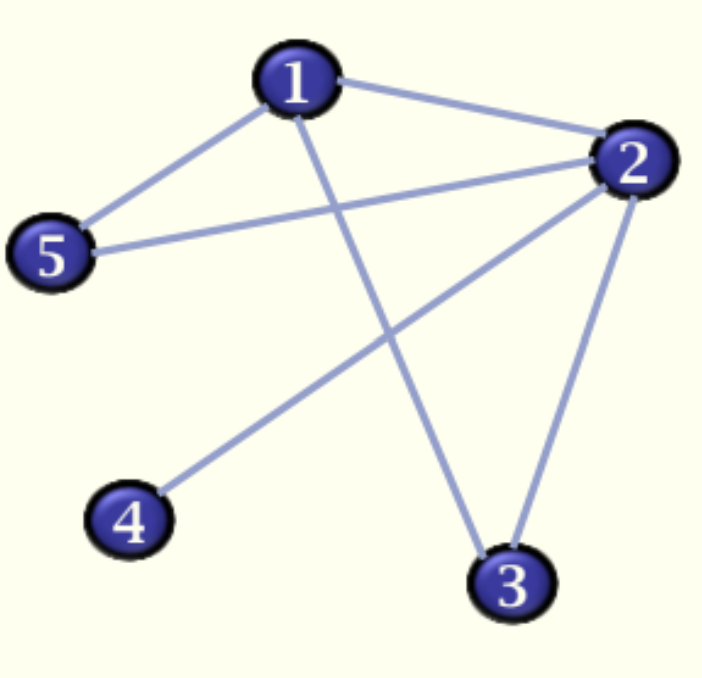
\includegraphics[width=0.2\textwidth]{images/graph_example.png}
\end{figure}
the efficiency is\begin{equation}
     E_g=\frac{2}{20}\left(
          1+1+\frac{1}{2}+1+1+1+1+\frac{1}{2}+\frac{1}{2}+\frac{1}{2}
     \right)=0.8.
\end{equation}
Given a specific node $i$ of a graph, we consider the graph composed by all the nodes directly connected to $i$ (but not including $i$ itself), denoted $S_i$ and compute its global efficiency $E_g(S_i)$.

The average of $E_g(S_i)$ across all the nodes is called \textbf{Local Efficiency} $E_l$ and measures the tendency of the network to form strongly connected
subgroups. It is also a measure of the robustness of the network to the removal of $i$.\begin{equation}
     E_l=\frac{1}{N}\sum_{i=1}^{N}E_g(S_i).
\end{equation}
\subsection{Graph Indices Used in Neuroscience}
For some applications it may be interesting to measure how well a
network can be divided into \textbf{communities}.
\begin{figure}[H]
     \centering
     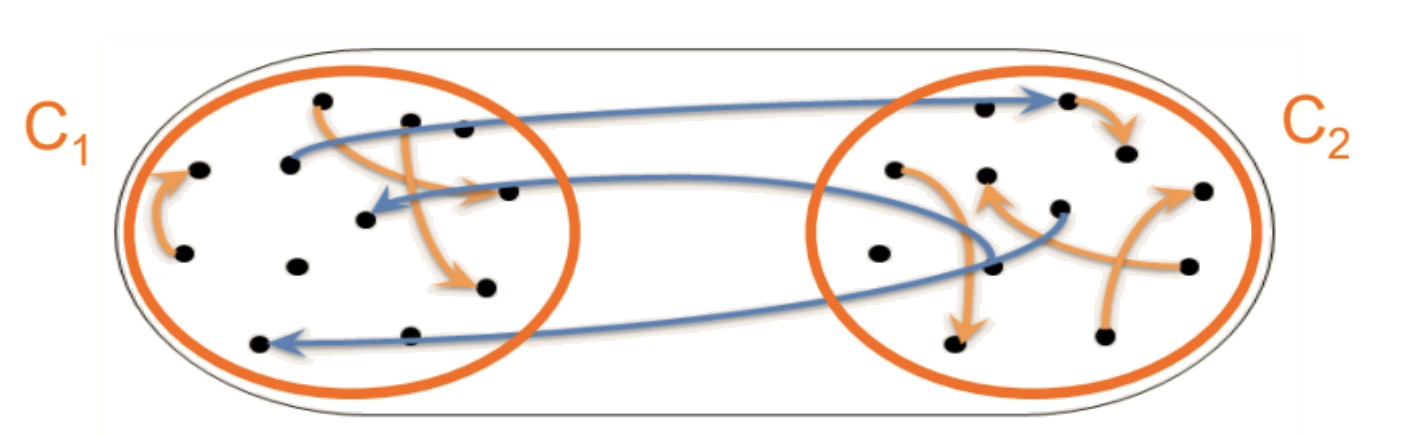
\includegraphics[width=0.5\textwidth]{images/community.png}
\end{figure} 
A subnetwork is a community if it shows an organized structure with
respect to the entire network. Measures useful to determine if two or
more subnetworks act as communities are \textit{Divisibility} and \textit{Modularity}.\bigskip 

The \textbf{Divisibility} $D$ is a measure of the \textit{segregation} between two given communities, for directed graphs is computed as:\begin{equation}
     D=\frac{2L}{\displaystyle 2L+\sum_{i=1}^{N}
     \sum_{j\ne i}^{N}a_{ij}(1-\delta(C_i,C_j))}
\end{equation}
for undirected graphs:
\begin{equation}
     D=\frac{L}{\displaystyle L+\sum_{i=1}^{N}
     \sum_{j\ne i}^{N}a_{ij}(1-\delta(C_i,C_j))}
\end{equation}
where \begin{itemize}
     \item $L$ is the number of edges in the network 
     \item $a_{ij}$ are the elements of the adjacency matrix
     \item $C_i$ is the community to which node $i$ belongs
     \item $\delta(C_i,C_j)=1$ if $C_i=C_j$, 0 otherwise.
\end{itemize}
Divisibility focuses on inter-community links.\bigskip

The \textbf{Modularity} $Q$ measures the tendency of the subnetworks to form communities. For undirected graphs:\begin{equation}
     Q=\frac{1}{2L}\sum_{i=1}^{N}
     \sum_{j\ne i}^{N}\left(
          a_{ij}-\frac{g_ig_j}{2L}  \right)\delta(C_i,C_j)
\end{equation}
for directed graphs:
\begin{equation}
     Q=\frac{1}{L}\sum_{i=1}^{N}
     \sum_{j\ne i}^{N}\left(
          a_{ij}-\frac{g_i^{IN}g_j^{OUT}}{2L}  \right)\delta(C_i,C_j)
\end{equation}
$g_i$ is the degree of a node  (can be of type $IN$ or $OUT$). Modularity focuses on intra-community links, gor each pair of nodes belonging to the same community, modularity $Q$ compares the
existence (or not) of a link between them with the probability of having a connection between them in a random distribution of the links:\begin{equation}
    \underbrace{ a_{ij}}_{\text{Existence of the
intra-community link}}-\underbrace{\frac{g_ig_j}{2L}}_{\text{Probability of a random link
between the nodes}}.
\end{equation}
If there are more intra-community links than in a random division, $Q>0$, otherwise $Q\le 0$.
We recap the properties of a graph under two labels:\begin{itemize}
     \item \textbf{Integration}:\begin{itemize}
          \item high global efficiency
          \item low local efficiency 
          \item low divisibility 
          \item low modularity.
     \end{itemize}
     \item \textbf{Segregation}:\begin{itemize}
          \item low global efficiency
          \item high local efficiency 
          \item high divisibility 
          \item high modularity.
     \end{itemize}
\end{itemize}
In general there are two \textit{reference structures} that describe  two different type of network:
\begin{center}
     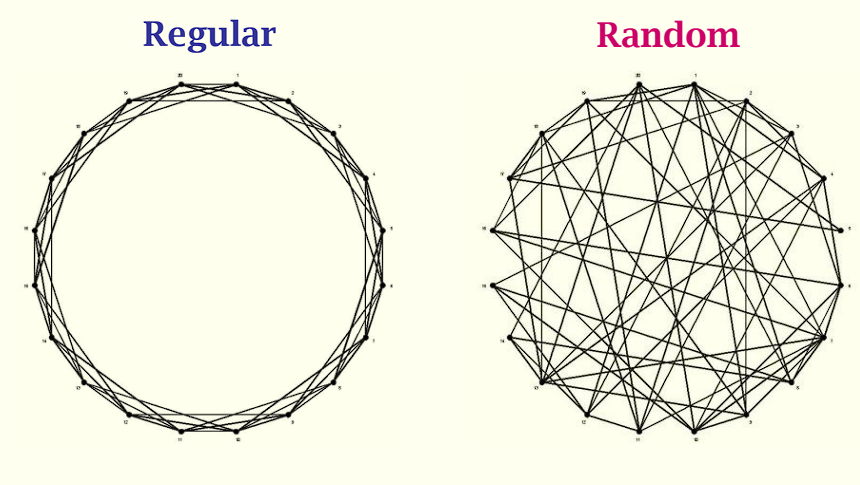
\includegraphics[width=0.45\textwidth]{images/regular_random.png} 
\end{center} 
\begin{itemize}
     \item Regular networks: Each node is linked to a small number of
other nodes.
The degree is the same for all nodes.
Efficient communications between small
groups, unefficient communications at the
entire network level.\begin{itemize}
     \item low Global Efficiency
     \item high Local Efficiency.
\end{itemize}
     \item Random networks: Each node is linked to the others
randomly. There are no small groups
with a strong internal communication.\begin{itemize}
     \item high Global Efficiency
     \item low Local Efficiency.
\end{itemize}
\end{itemize} 
Real world networks are neither like the random nor like the regular graphs.
\section{Multiple-Subject Systems}
Human-to-human interactions are important in:\begin{itemize}
     \item human cognition, development, well-being, society
\end{itemize}
and are extremely complex, due to unpredictable time trajectory, they require social settings and include dynamic stimulation involving a
large set of complex sensory features (face expressions,
gestures, postures, actions, intonation). These are usually based on alignment:\begin{itemize}
     \item bodily synchrony 
     \item turn taking during conversation 
     \item similar orientation of attention 
     \item empathy.
\end{itemize}
These interactions can be non verbal, dynamic and bilateral, they can have a leader-follower setting or can be symmetrical.\begin{itemize}
     \item A complex system (group) cannot be
     fully understood by analyzing its
     single elements (single subjects): we
     need to study their interaction.
     \item The content and timing of natural
social interaction are unpredictable
and differ from experiment to
experiment.
     \item Interdependencies between the two
sets of brain signals can reveal brain
processes that support the interaction.
\end{itemize}
\begin{center}
     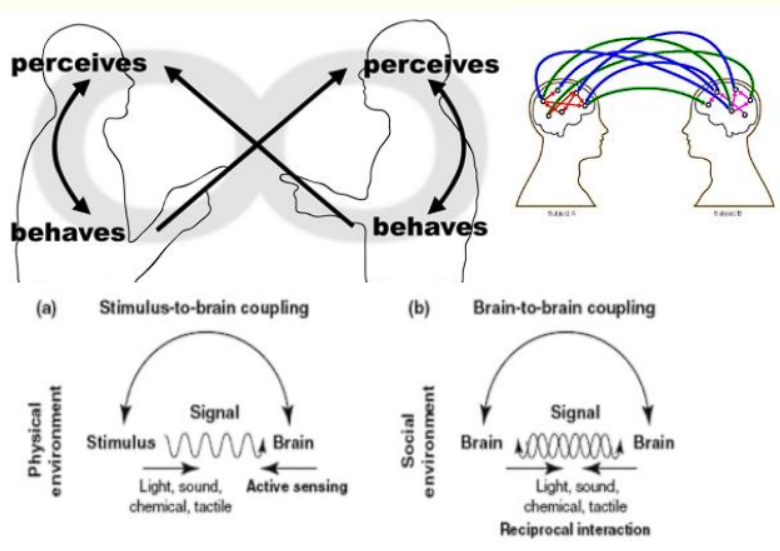
\includegraphics[width=0.5\textwidth]{images/human_interaction.png} 
\end{center} 
We can use the tools of graph theory and apply them to the analysis of multi-subject systems, with the aim of quantifying brain interaction not only within the brain of a single individual, but between the brains of two or more subjects interacting with each other.
\begin{center}
     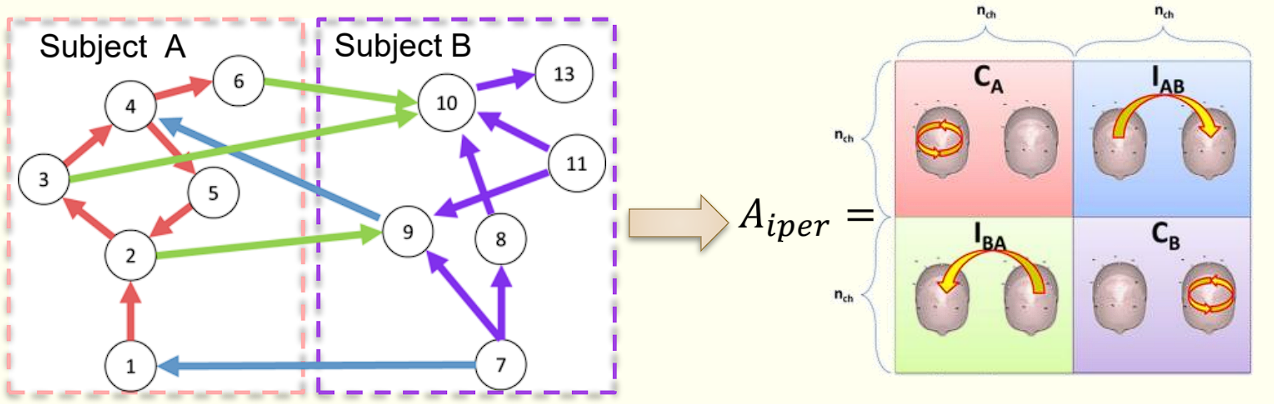
\includegraphics[width=0.6\textwidth]{images/multisubject.png} 
\end{center} 
the brain activity of two subjects can be modeled as a single large interconnected system: The nodes represent the channels or electrodes (e.g. EEG) positioned on the scalp of the two subjects, the arcs represent connectivity (e.g. synchronization or information flow). To extract biological and behavioral information from this hyper-graph, the properties seen previously (modularity, divisibility, efficiency) are considered.\bigskip
\subsection{Cooperation and Competition}
Observe the following picture:
\begin{figure}[H]
     \centering
     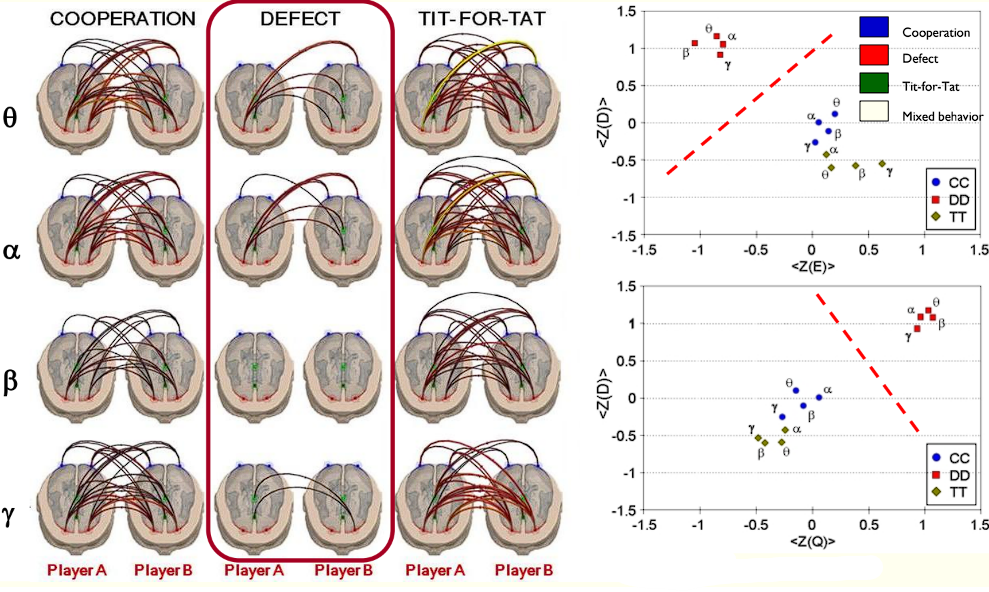
\includegraphics[width=0.8\textwidth]{images/game_theory_system.png} 
     \caption{Application in game theory.}
     \label{coperation_defect}
\end{figure} 
This picture shows the practical application of the inter-subject graph concepts seen previously, applied to a game theory context (typically the repeated Prisoner's Dilemma), analyzing how brain connectivity patterns change depending on social behavior.
The left part of Figure \ref{coperation_defect} shows the connectivity networks calculated between two players (Player A and Player B) based on four different EEG frequency bands (brain waves):\begin{itemize}
    \item $\theta$ (Theta): Linked to complex cognitive processes and working memory.\item $\alpha$ (Alpha): Linked to attention and resting/alert states.\item $\beta$ (Beta): Linked to motor activity and active concentration.\item $\gamma$ (Gamma): Linked to multisensory integration and high-level cognitive processes.
\end{itemize}\begin{itemize}
     \item \textbf{Cooperation and Tit-for-Tat}: They show a dense network of lines (graph arcs) that intensely connect the brain of Player A with that of Player B. This indicates strong inter-subject synchronization and a continuous exchange of information; the two brains ''work together''.
     \item \textbf{Defect}: When players compete or cheat on each other, the lines between the two brains decrease dramatically in all frequency bands. There is very little inter-subject connectivity: each acts independently and selfishly, disrupting the shared ''super-brain''.
\end{itemize}
On the right side of Figure \ref{coperation_defect}, the two graphs show how, using graph metrics calculated on the networks, it is possible to mathematically separate and classify the three behaviors.
On the abscissas and ordinates we find the normalized values ($Z$-score) of the metrics seen in the previous picture:\begin{itemize}
     \item $<Z(D)>$:Average divisibility. \item $<Z(E)>$: Average global efficiency. \item $<Z(Q)>$: Average modularity.
\end{itemize}
The red squares (DD - Mutual Defection) are positioned in a completely different area compared to the blue circles (CC - Cooperation) and the green diamonds (TT - Tit-for-Tat).

The red dotted line represents a linear separation hyperplane (decision boundary). It shows that graph theory metrics applied to hyperscanning are so powerful that they allow us to clearly distinguish cooperative behavior from competitive behavior.

\textbf{Conclusion}: By combining these frequency bands ($\theta, \alpha, \beta, \gamma$) and network metrics, a machine learning algorithm can guess with 91\% accuracy whether the pair is cooperating, competing, or implementing a tit-for-tat strategy, based solely on the combined electrical activity of their brains.
\subsection{Empathy}
Empathy is here divided and mapped into two distinct macro-phenomena:\begin{itemize}
     \item Compassion: it is the emotional response we feel when we see another human being suffer or suffer an injustice. It is defined as ''negative'' because it is linked to sharing a state of discomfort or pain in others.
     \item Vicarious Reward: it is the feeling of gratification we feel when we see the other person doing well or receiving a fair reward/treatment. It is defined as ''positive'' because it activates the brain's reward systems even if the benefit is not directed to us.
\end{itemize}
\begin{figure}[H]
     \centering
     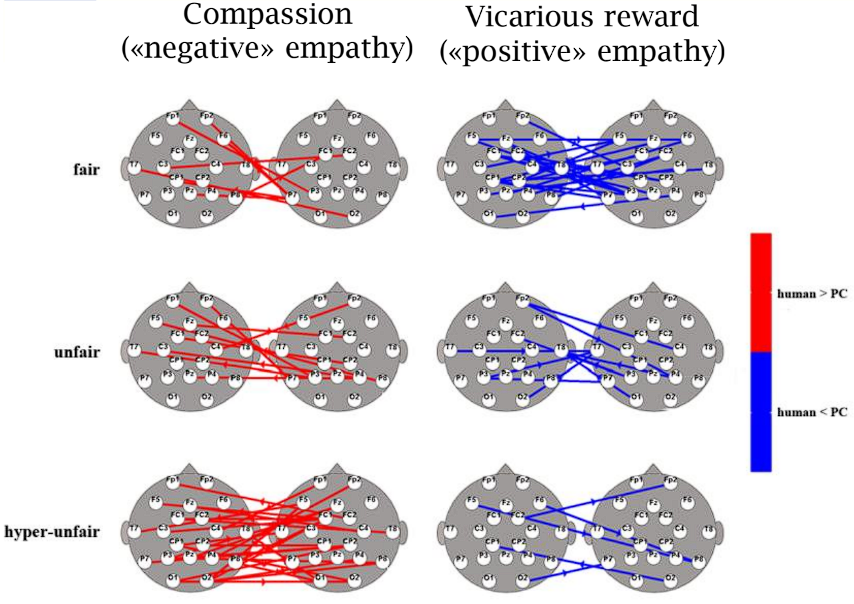
\includegraphics[width=0.6\textwidth]{images/empathy.png} 
     \caption{Empathy effects on the EEG.}
     \label{empathy}
\end{figure} 
The experiment in Figure \eqref{empathy} evaluates how inter-subject brain connections change by manipulating the level of fairness of the economic or social treatment suffered by one of the participants:\begin{itemize}
     \item Fair: Correct and balanced treatment.
 \item Unfair: Slightly unfair treatment.
 \item Hyper-unfair (Extremely unfair): Blatantly and grossly unfair treatment.
\end{itemize}
As iniquity increases (going down the lines): You notice a dramatic increase in red connections in the Compassion column. In the hyper-unfair condition, the network of inter-subject connectivity linked to compassion becomes very dense. The brain of the observer becomes strongly attuned to the brain of the victim of injustice.
On the contrary, for Vicarious Reward (blue lines): Connections tend to reduce when the situation becomes extremely unfair, as the shared gratification component disappears.\bigskip

The indices of the brain graph are modulated by the level of empathy between the subjects (measured by the level of fairness of the treatment suffered by one of them and by the consequent altruistic help provided by the other).

\begin{boxobservation}{}{}
      The connectivity between the two brains is not static, but varies in a predictable and quantifiable way.
\end{boxobservation}
The more unfair the treatment suffered by a subject, the greater the cerebral empathy measured by the graphs.

This emotional ''hyper-graph'' is directly proportional to subsequent behavior: a strong brain tuning linked to compassion predicts how inclined the second subject will be to offer altruistic help to defend or compensate his partner.
\subsection{Joint Action}
Joint action can be analyzed by studying how two people's brains coordinate at a neural level when they have to perform a motor or cognitive task together, compared to when they do it alone or against a computer.
\begin{figure}[H]
     \centering
     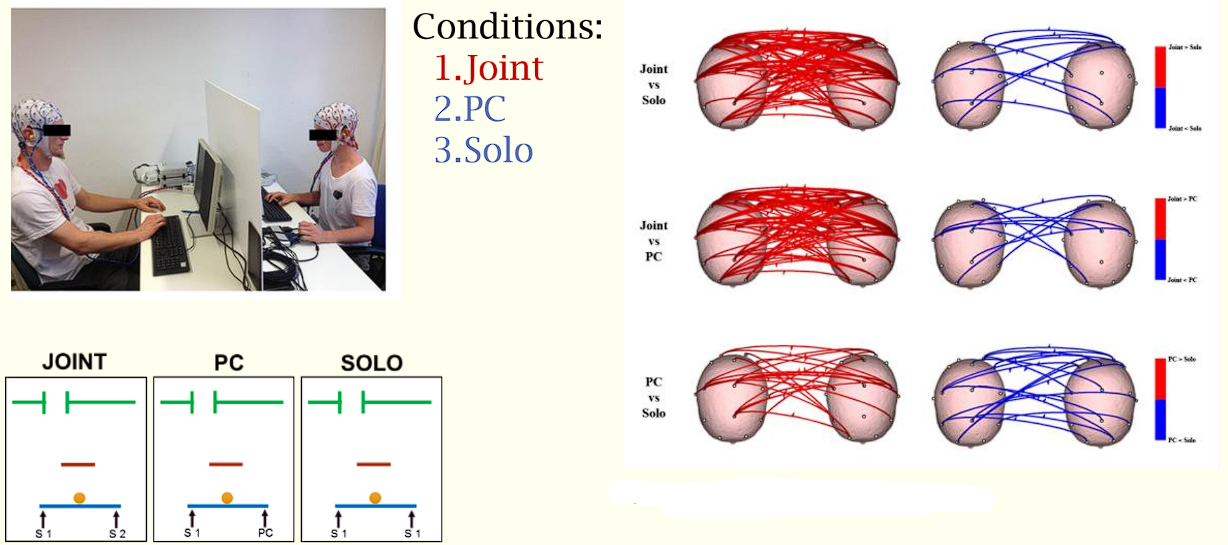
\includegraphics[width=0.8\textwidth]{images/joint_action.png} 
     \caption{Recording EEG during joint action (1).}
     \label{jointaction}
\end{figure} 
In Figure \ref{jointaction} are reported three configurations:\begin{itemize}
     \item Joint vs Solo: In red ($Joint > Solo$): Shows a huge density of inter-subject connections. When people act together, their brains show a hyper-coordinated level of synchronization that is biologically absent when they act alone. In blue ($Joint < Solo$): Shows very few connections, confirming that the solo condition breaks down the network synchrony between the two EEG heads.\item Joint vs PC: This is the most important contrast: it shows that the human brain recognizes the intentionality of the other human being. Even if the task performed with the PC is identical from a motor point of view, the inter-subject connectivity is significantly stronger and more extensive in the Joint case (morphology in red). Interacting with artificial intelligence or software does not evoke the same level of brain attunement.
     \item PC vs Solo (Third row):Shows the difference between playing with a computer and playing alone. There is a slight increase in connectivity due to the presence of an external agent (the PC that responds to actions), but the effect is decidedly smaller than the contrast with real human interaction (Joint).
\end{itemize}
\begin{boxobservation}{}{}
     Joint action between humans creates a unique and specialized neural coupling. Our brain does not simply process stimuli and produce motor responses, but ''locks'' to that of our social partner, establishing a shared and extensive neural network that is not activated when we interact with a machine.
\end{boxobservation}
\begin{figure}[H]
     \centering
     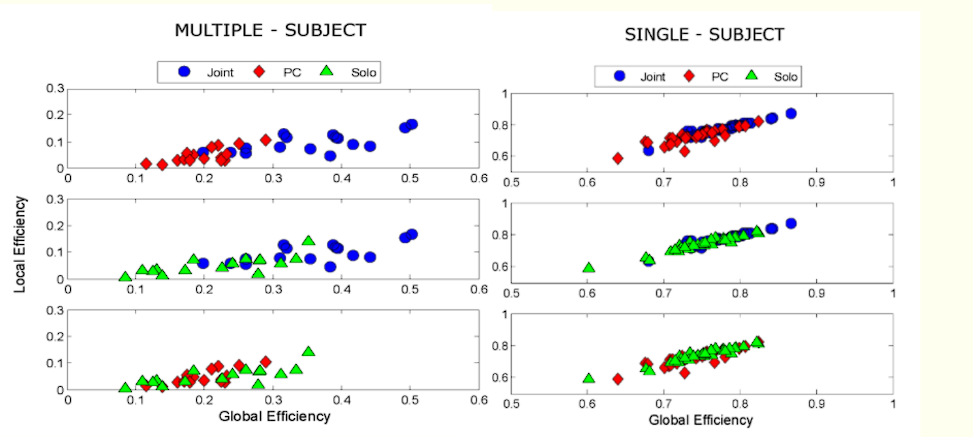
\includegraphics[width=0.6\textwidth]{images/joint_action2.png} 
     \caption{Recording EEG during joint action (2).}
     \label{jointaction2}
\end{figure} 
Figure \ref{jointaction2} shows the quantitative results of the Joint Action study, comparing two different graph analysis methods: Multiple-Subject analysis (Hyper-brain on the left) and Single-Subject analysis (Single-brain on the right).\begin{itemize}
     \item Multiple-Subject Analysis: By treating the two brains as a single ''hyper-graph'', the Joint condition (cooperation between humans) clearly separates itself from the others. It shows much higher Global and Local Efficiency values, highlighting a unique and optimized information exchange that does not occur when playing alone or with a computer.
     \item Single-Subject Analysis: If the brain of only one subject is analyzed at a time, the points of the three conditions (Joint, PC, Solo) are completely overlapped and indistinguishable.
\end{itemize}
The classic analysis on the single subject fails to detect social cooperation. Human neural coupling becomes visible and measurable only through the mathematical metrics of the Hyper-brain.\bigskip

One experiment involved 4 subjects simultaneously recorded via EEG while they played cards:
\begin{figure}[H]
     \centering
     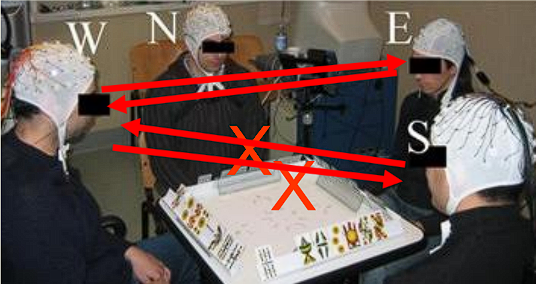
\includegraphics[width=0.5\textwidth]{images/cardgame1.png} 
\end{figure} 
\noindent Two conditions were compared:\begin{itemize}
     \item Baseline: The analysis of all possible pairs sitting at the table in the same session.
\item Cooperation: The targeted analysis of pairs that belong to the same team. The task is asymmetrical and is divided between a ''first player'' (Leader) and a ''second player'' (Follower). The red arrows with the ''X'' in the photo indicate that the relevant connectivity is not between opponents, but between teammates.
\end{itemize}
The graphs show the directional connectivity between the brain areas (e.g. ACC - Anterior Cingulate Cortex, BA8, BA9, BA10, BA7) of the two teammates in two frequency bands: the Beta band (concentration/motor task) and the Gamma band (complex cognitive integration).
\begin{itemize}
\item Information flow (Directed arrows): There is a clear directionality of the arrows starting from the top (Leader's brain areas) and going downwards (Follower's brain areas).
\item Biological meaning: In cooperating couples, the brain of the person leading the action (Leader) ''modulates'' and directly influences the brain activity of the person who must respond or follow the strategy (Follower).
\end{itemize}
\begin{figure}[H]
     \centering
     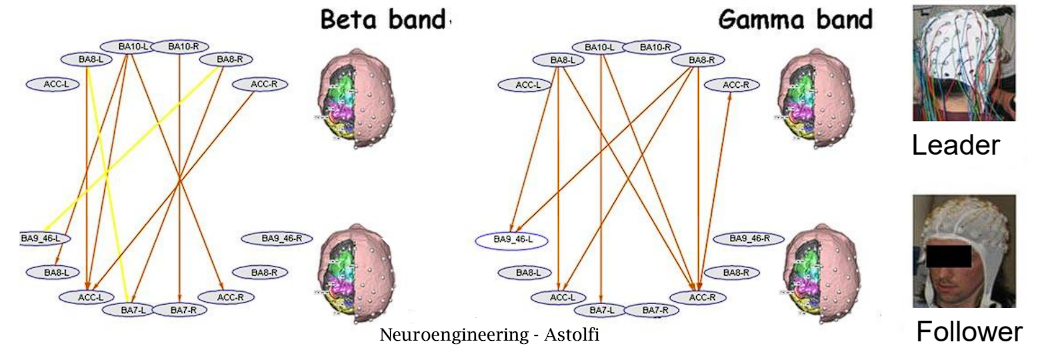
\includegraphics[width=0.8\textwidth]{images/cardgame2.png} 
\end{figure} 
In summary: Even in complex real-world 4-player contexts, graph theory applied to hyperscanning is able to map inter-personal information flows, revealing the implicit functional hierarchy (Leader-Follower) within a cooperating team.\bigskip 

Another study was performed outside the classical laboratory to analyze brain synchronization in a realistic scenario:\begin{itemize}
     \item The Subjects: 12 professional pilots, divided into 6 pairs each made up of a Captain and a First Officer.

\item The Instrumentation: Each pilot is monitored simultaneously with 15 EEG and ECG electrodes during a 90-minute simulated flight session.

\item The Objective: Manipulate the instrumentation and insert unexpected events during the flight to induce different levels and types of interaction and cooperation between the two pilots.
\end{itemize}
I grafi mettono a confronto l'attività cerebrale combinata della coppia in base alle fasi di volo e al livello di cooperazione richiesto\begin{itemize}
     \item  High Cooperation : During the critical phases of take-off and landing, a dense network of connections (colored lines) is observed that connect the two brains. There is a clear directionality of information flows that move mainly from the First Officer to the Captain or vice versa, depending on the specific coordination and communication tasks necessary to maneuver the aircraft safely.
     \item  No Cooperation: In the phases of rest or execution of individual decoupled tasks (Rest-BCI and BCI-rest), the inter-subject connections almost completely disappear. The two brains return to functioning as isolated entities.
\end{itemize}
\begin{figure}[H]
     \centering
     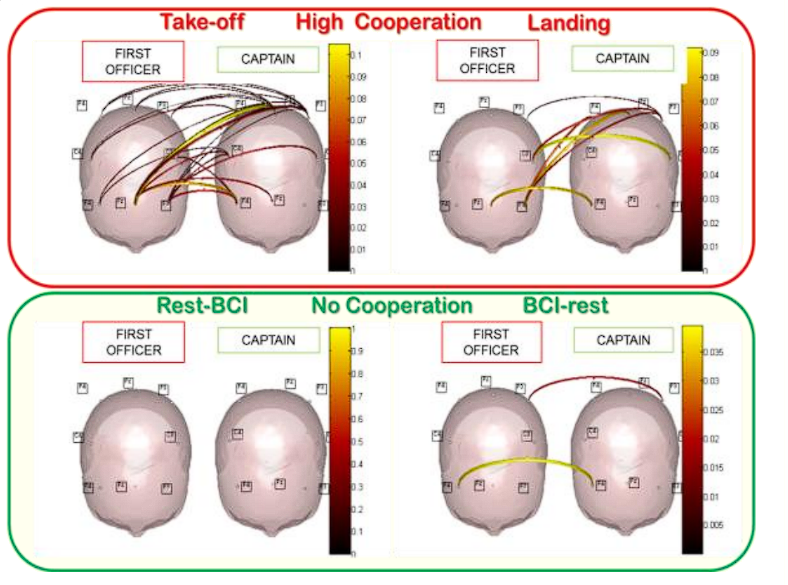
\includegraphics[width=0.6\textwidth]{images/pilots.png} 
\end{figure} 
\subsection{Future Directions}
\begin{itemize}
     \item Study of the development of cognitive functions in
children and their modifications in psychiatric and
behavioral disorders (Autism Spectrum Disorders).
\item New approaches to:\begin{itemize}
\item Rehabilitation of cognitive functions in
pathological conditions.
\item Enhancement of social skills.\end{itemize}
\item Definition of brain indices as outcome measures to
quantify/describe the effect of a
rehabilitative/enhancement intervention.
\item Social robotics: robots with human-like skills
(able to mimic but also to interact with humans
in a natural way).
\end{itemize}
\chapter{Neuroscience Applications}
\section{Introduction}
Neuroengineering operates at the intersection of neuroscience, bioengineering, robotics, control engineering, and computer science. Its primary overarching aim is the design and development of innovative devices capable of replacing or restoring motor, cognitive, or sensory functions that have been compromised due to pathological conditions or traumatic events. A defining characteristic of neuroengineering solutions is the direct interfacing of these technological devices with the central or peripheral nervous system. This chapter explores the major applications of this multidisciplinary field, organized into four primary pillars: neurorehabilitation, neuroprosthetics and orthotics, and assistive technologies.

\section{Neurorehabilitation and Motor Learning}
Neurorehabilitation strategies are fundamentally anchored in the concept of \textit{neuroplasticity}---the brain's innate capacity to self-repair and reorganize by modifying synaptic connectivity patterns. These neuroplastic modifications are highly dependent on the stimuli the brain receives, the physical activities performed, and the overall sensory experience of the individual.
\begin{figure}[H]
     \centering
     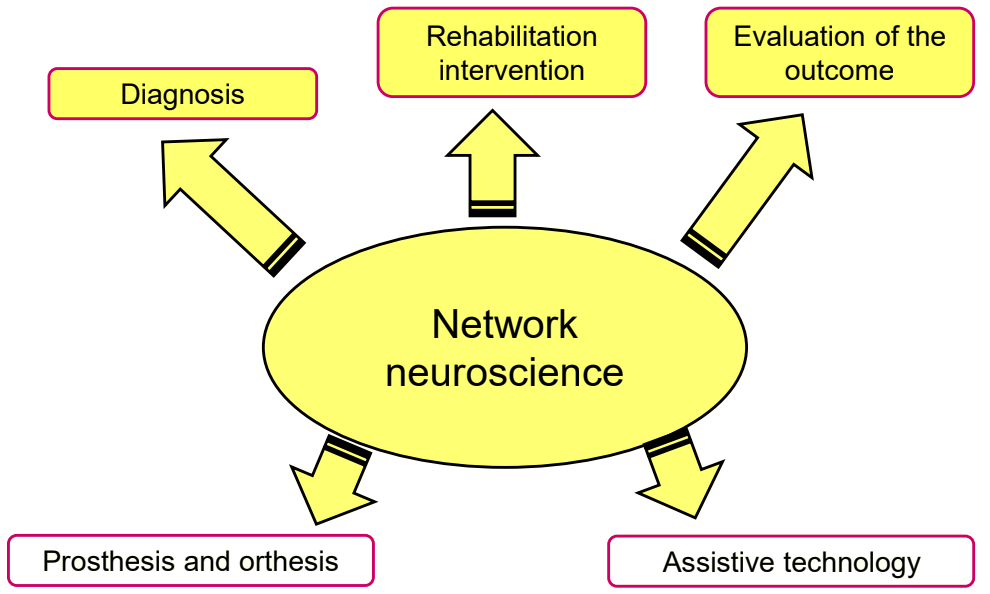
\includegraphics[width=0.4\textwidth]{images/applications_1.png} 
\end{figure} 
\subsection{Principles of Motor Learning}
The acquisition and refinement of motor control occur predominantly through a trial-and-error process. Crucially, motor learning relies on the concept of \textit{prediction error}: the quantifiable difference between the outcome anticipated by the brain's internal forward models and the actually observed movement outcome. 
Motor learning is triggered both in response to external environmental perturbations and to internal bodily modifications that generate these movement errors. Importantly, post-injury recovery processes heavily rely on the same mechanisms that govern normal motor learning.

\subsection{The Role of Feedback}
Feedback mechanisms are indispensable for continuous learning and neural reorganization. This feedback is typically categorized into two forms:
\begin{itemize}
    \item \textbf{Intrinsic Feedback:} Provided autonomously by the patient's own sensory systems (proprioceptive, visual, tactile), enabling the internal evaluation of performance for each executed movement.
    \item \textbf{Extrinsic (Augmented) Feedback:} Provided by an external source or clinical device, supplying additional, often quantitative, information regarding the quality of the movement.
\end{itemize}

\section{Evaluation of Rehabilitation Outcomes}
Accurate diagnosis and ongoing evaluation are critical components of the rehabilitation lifecycle.

\subsection{Functional Evaluation}
The clinical assessment of motor ability is traditionally quantified through standardized clinical scales, such as the Barthel Index, the Motricity Index, and the Fugl-Meyer Assessment. These instruments assign specific scores to distinct body regions and movement types, allowing clinicians to compare a patient's motor capability against normative data.

\subsection{Neurophysiological Evaluation}
Beyond functional scales, neuroengineering facilitates the direct evaluation of brain plasticity. For instance, post-stroke recovery can be monitored using electroencephalography (EEG) screening. Advanced network neuroscience techniques reveal that Brain-Computer Interface (BCI)-supported training can induce quantifiable increases in inter-hemispheric connectivity. Furthermore, specific graph-theoretical indices of brain networks have demonstrated strong correlations with improvements in functional clinical outcomes.
\begin{figure}[H]
     \centering
     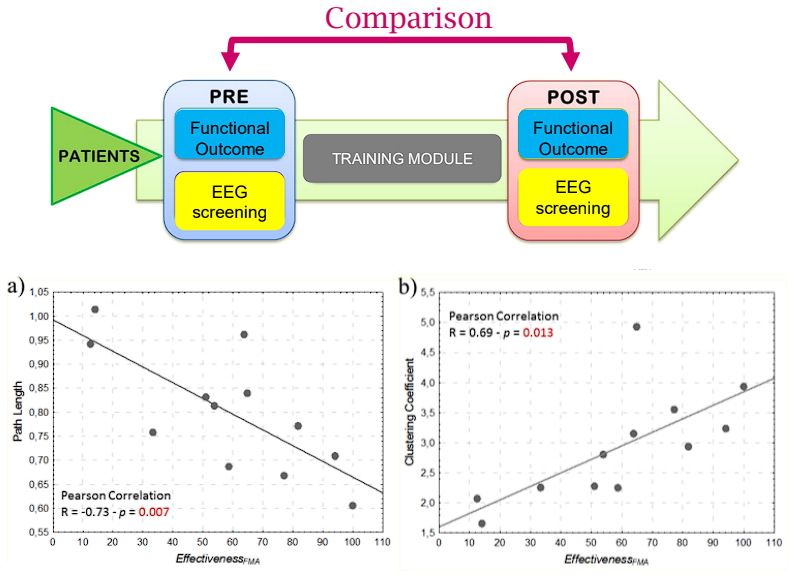
\includegraphics[width=0.5\textwidth]{images/application_2.png} 
\end{figure} 
\section{Innovative Therapeutic Interventions}
Conventional rehabilitation is increasingly augmented by advanced technological interventions, which provide higher intensity, better engagement, and precise quantification.

\subsection{Brain-Computer Interfaces (BCI)}
BCI-based rehabilitation allows for the deliberate and controlled activation of specific brain cortical areas. One of the most significant advantages of this approach emerges when a patient can successfully activate the appropriate neural motor commands but cannot physically execute the movement due to paralysis or weakness. In such cases, the BCI detects the correct neural intent and triggers a motivating reward. If the impaired limb is coupled to a robotic orthosis, the device can physically complete the intended task, closing the sensorimotor loop and reinforcing synaptic plasticity.

\subsection{Robotics and Virtual Reality}
Robotic devices applied to the upper and lower limbs offer multifaceted advantages:
\begin{itemize}
    \item \textbf{Precise Measurement:} They accurately quantify movement kinematics (e.g., position, acceleration) and dynamics (force) throughout the recovery trajectory.
    \item \textbf{Controlled Environments:} Robot-assisted therapy ensures absolute control over task timing, environmental stimuli, and the delivery of augmented feedback (biofeedback).
    \item \textbf{Cost and Intensity:} They facilitate the delivery of highly intensive, repetitive therapeutic regimens at a potentially lower long-term cost compared to solely manual conventional therapies.
\end{itemize}
Concurrently, Virtual and Augmented Reality (VR/AR) environments immerse the patient in engaging, realistic scenarios, significantly increasing attentional focus and motivation during repetitive motor tasks.
\begin{figure}[H]
     \centering
     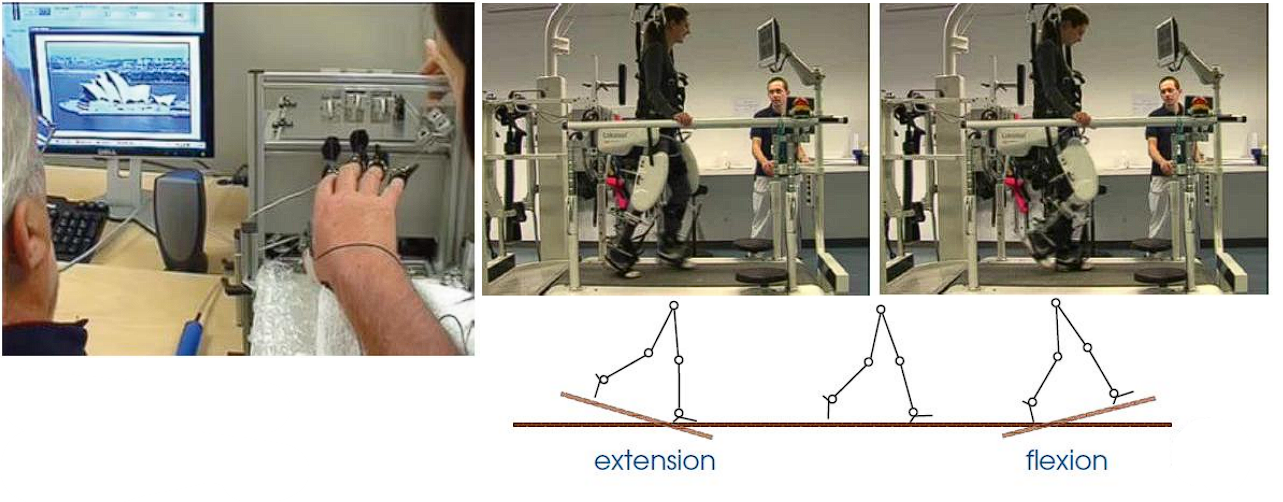
\includegraphics[width=0.7\textwidth]{images/application_3.png} 
\end{figure} 
\subsection{Cognitive Rehabilitation}
Neuroengineering is not restricted to motor domains. Cognitive rehabilitation utilizes physiological correlates (such as EEG sensorimotor rhythms, ECG, and Heart Rate Variability) to provide real-time neurofeedback. By presenting patients with visual or auditory representations of their brain states, home-based or remote-controlled systems can train sustained attention and rehabilitate memory functions following a stroke.
\begin{figure}[H]
     \centering
     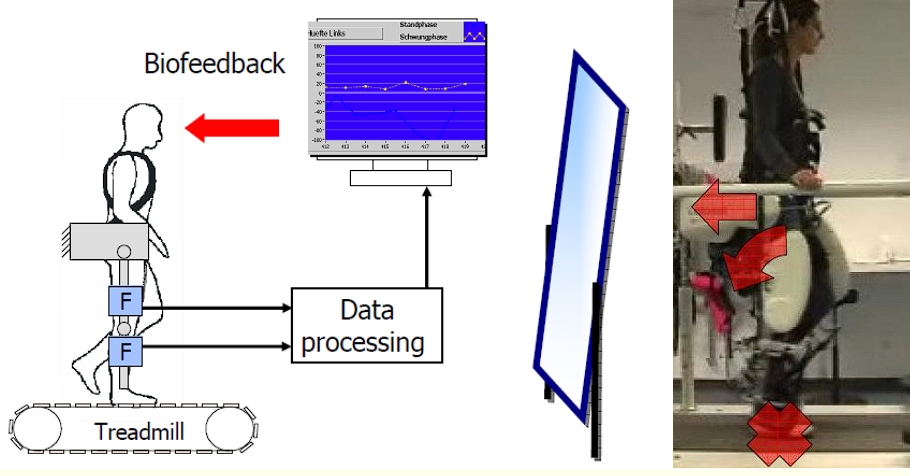
\includegraphics[width=0.7\textwidth]{images/application_4.png} 
\end{figure} 
\section{Neuroprosthetics and Orthotics}
When endogenous recovery is insufficient, neuroprostheses aim to artificially restore lost capacities. These interventions are broadly categorized based on the direction of information flow.
\begin{figure}[H]
     \centering
     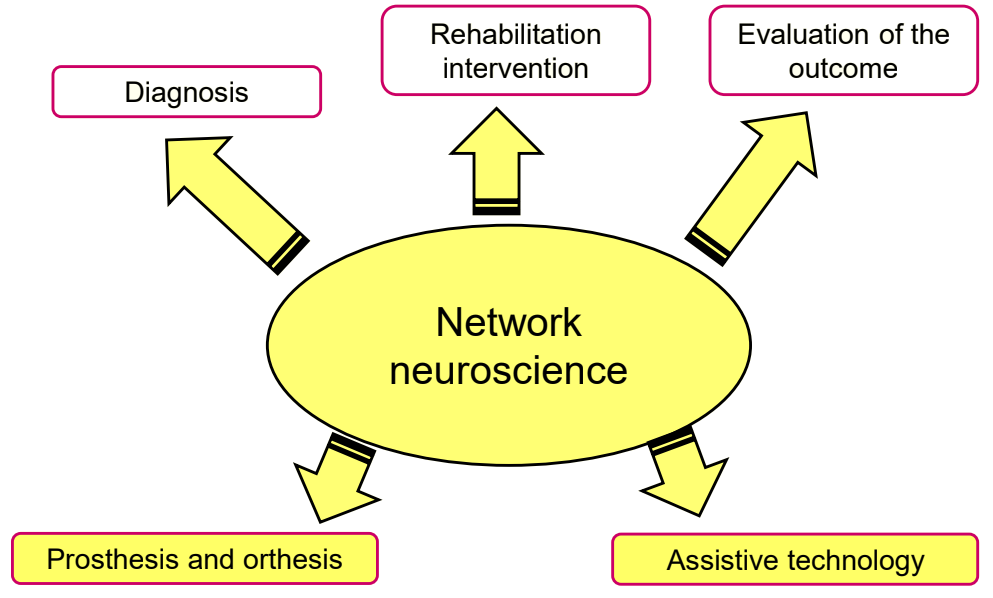
\includegraphics[width=0.4\textwidth]{images/applications_5.png} 
\end{figure} 
\subsection{Input (Sensory) Prostheses}
Input prostheses measure external physical signals and convert them into neural perceptions via targeted electrical stimulation.
\begin{itemize}
    \item \textbf{Auditory Neuroprostheses:} The cochlear implant is the most established sensory prosthesis (in use since 1957). It consists of external components (microphone, speech processor, transmitter) and internal implanted components (receiver and stimulator arrays). The internal electrodes directly stimulate the acoustic nerve, effectively restoring hearing function.
    \item \textbf{Visual Neuroprostheses:} Aimed at restoring vision in conditions like macular degeneration. They involve capturing an image, encoding the visual stimulus, and transmitting this data to a microelectrode array implanted in the visual cortex or retina, thereby eliciting visual percepts.
\end{itemize}
\begin{figure}[H]
     \centering
     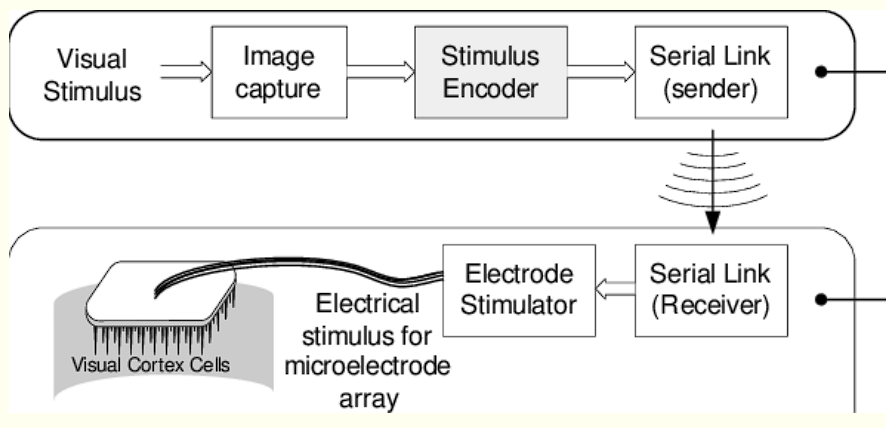
\includegraphics[width=0.4\textwidth]{images/visual_recovery.png} 
\end{figure} 
\subsection{Output (Motor) Prostheses}
Output prostheses decode brain signals to translate user intentions into physical actions. These include artificial limbs, exoskeletons, or Functional Electrical Stimulation (FES) orthoses. FES systems operate by delivering an electrical current directly into a paralyzed muscle to evoke controlled contractions (e.g., to restore hand grasp).
Advanced setups rely on multichannel neural signal processing, where data from implanted microelectrode arrays is transmitted via telemetry, translated into 3D movement trajectories, and used to drive a robotic arm in real-time.

\section{Assistive Technologies}
Beyond direct medical rehabilitation and functional replacement, neuroengineering significantly contributes to assistive technologies designed to improve overall quality of life. For patients with severe motor impairments (e.g., locked-in syndrome), non-invasive BCI systems can be integrated into daily software, providing alternative channels for communication (e.g., BCI-driven spelling applications) and facilitating digital social interaction.

\chapter{Measurement of Bioelectrical Signals}
\section{The Electroencephalogram}
In the 1920s and 1930s, the research about non invasive measurements of signals from the scalp began to progress significantly, in particular, a reports published by Hans Berger (Germany) was able to demonstrate a large and persistent 10 Hz rhythm that he named the ''alpha'' rhythm. Lord Adrian, a british neuroscientist, found that these alpha oscillation appeared only when the occipital cortex had a ''small workload'', in particular, when the eyes are shut and there is no visual information to process, suggesting that these oscillation they are the consequence of an state.\begin{center}
     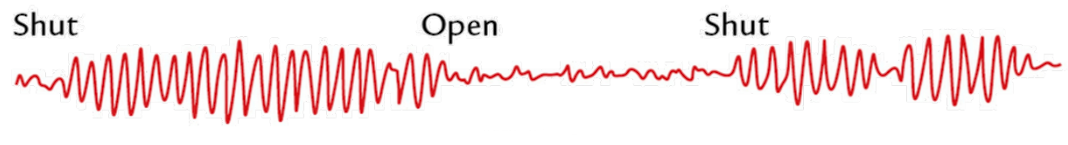
\includegraphics[width=0.8\textwidth]{images/idling_alpha.png} 
\end{center} 
The \textbf{electroencephalogram} (EEG) is the measurements of the electrical activity of the brain, that can be measure by putting a set of \textit{electrodes} on the scalp. The activity of a single neuron is imperceptible to our instruments, but when multiple neurons starts to work in ''combination'' some variations of electrical potential can be observed.
\begin{boxdefinition}{Synchronization}{}
    In the context of neuroscience, we say that the EEG \textbf{synchronize} when the amplitude of the registered wave increase.
\end{boxdefinition}
The brain can be seen as a complex, non-linear and time variant dynamical system, the registered waves on the scalp are the reaction to a given ''input''. The registered oscillation are different between different execution of the same input, so usually more registration of the same input are taken to construct the average EEG signal, time locked to various sensory stimuli, thereby significantly
increasing the signal-to-noise ratio.\bigskip

We talk about \textbf{Event Related Potential} when a change in the electrical potential is registered immediately after a given input to the brain (for example, a flash light turning on in front of the eyes), there are also spontaneous rhythm that doesn't needs a time defined event. The already mention averaging procedure is essential to distinguish between the spontaneous rhythm, the ERP, and the electrical noise (also called signal's ''artifacts'').\bigskip

As we already mentioned, the EEG is measured through  an electrode, this is basically a very sensible voltmeter, that captures the changes in the electrical potential on the surface where it's placed, usually, a large number of electrodes are placed on the head (up to 256), to measure the signal over time for each electrode.
\begin{center}
     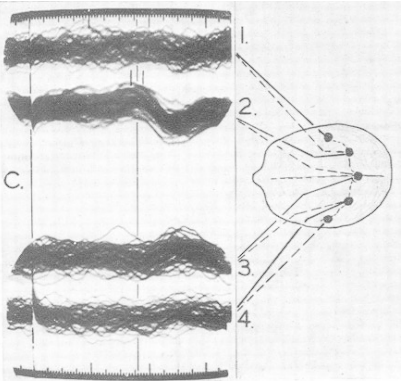
\includegraphics[width=0.3\textwidth]{images/averaging.png}
     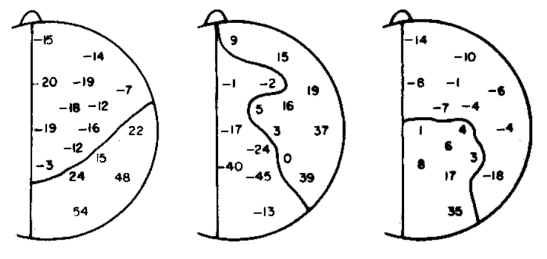
\includegraphics[width=0.6\textwidth]{images/potential_scalp.png} 
\end{center} 
The following image shows the displacement of three groups of electrodes (2 for each group) placed in different areas of the head.
\begin{center}
     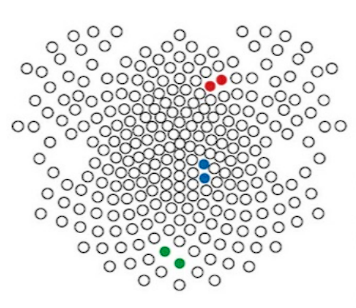
\includegraphics[width=0.3\textwidth]{images/electrode_displacement.png}
\end{center} 
The red electrodes are placed in an area near the cheeks, the blue electrodes are placed on the top of the head, on the motor cortex, and the green one are placed on the occipital cortex. Let's consider the following signals:\begin{center}
     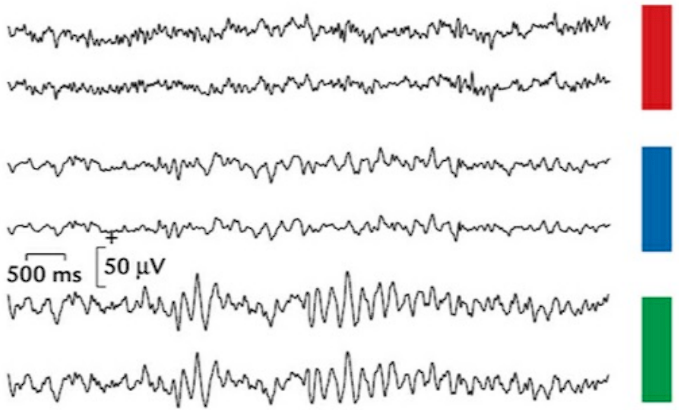
\includegraphics[width=0.35\textwidth]{images/alpha_waves.png}
\end{center} 
we can observe how the electrodes placed on the occipital cortex synchronize at some points, and start oscillating around 10 Hz, these are the so called \textbf{alpha rhythm}, mainly registered on the occipital cortex, the other electrodes doesn't seem to register any reaction. The following signals are registered when the muscle of the subject are completely still:
\begin{center}
     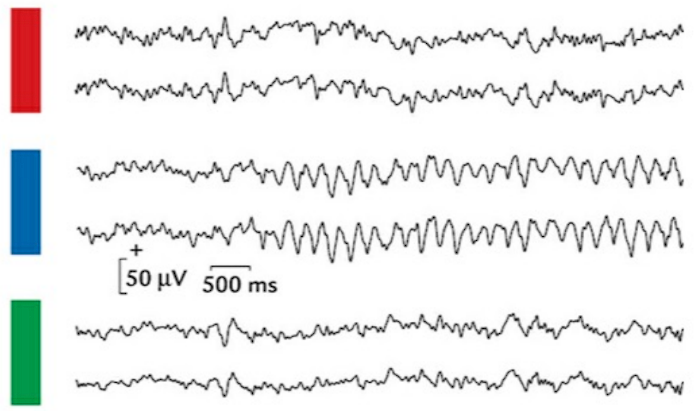
\includegraphics[width=0.35\textwidth]{images/mu_waves.png}
\end{center} 
We can observe how the electrodes placed on the motor cortex reacts, these oscillation are directly connected to the motor system. It is recorded in very specific conditions that concern the ''rest'' state of the muscles and movement planning.\bigskip

\textit{About the axes}: In every EEG there are two small ''bars'', called \textit{calibration bars}, these are needed to show the scale of the timeline and the amplitudes of the signals. From the alpha and the mu rhythm we can see how the ERP are in the order of micro volts [$\mu V$].
\begin{center}
     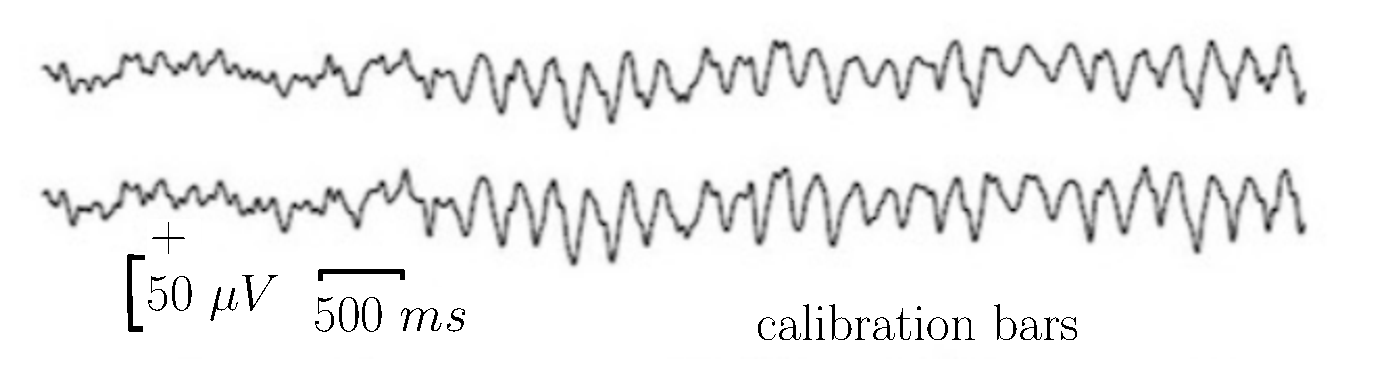
\includegraphics[width=0.4\textwidth]{images/cal_bars.eps}
\end{center} 

We categorize the observed signals in base of their frequency, by considering 5 different bands.
\begin{itemize}
    \item Delta: less than 3.5 Hz 
    \item Theta: from 4 to 7.5 Hz
    \item Alpha: from 8 to 13 Hz 
    \item Beta: from 14 to 30 Hz 
    \item Gamma: more than 30 Hz
\end{itemize}
Clearly, the alpha rhythm is in the alpha band (around 8 to 13 Hz), also the mu rhythm is in the same band, it might be confusing, it is important to remember than the word ''bands'' refers only to the frequency, and not to other properties of the observed rhythm (like the areas where are registered).\begin{center}
     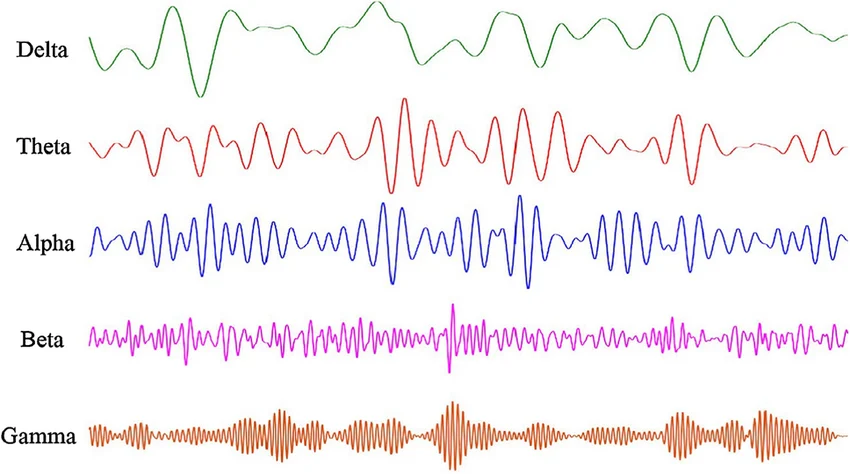
\includegraphics[width=0.5\textwidth]{images/bands.png}
\end{center} 
\begin{boxdefinition}{ERP}{}
     An \textbf{Event Related Response (ERP)} is a potential related to an event (cognitive input) to the brain, the time that the brain takes to react depend of the kind of input, and can range from a few milliseconds to hundreds of milliseconds, usually the ''fastest'' response comes from the \textit{primal areas}, that are the earlier in the stage of processing.
\end{boxdefinition}
\begin{boxdefinition}{Trial}{}
     A \textbf{trial} is a segment of the EEG after a sensory stimulus, and the latency is the time delay between the stimulus and the trial, as we already mentioned, we takes many individual trial and then average the data to see the global response. 
\end{boxdefinition}
\begin{figure}[H]
     \centering
     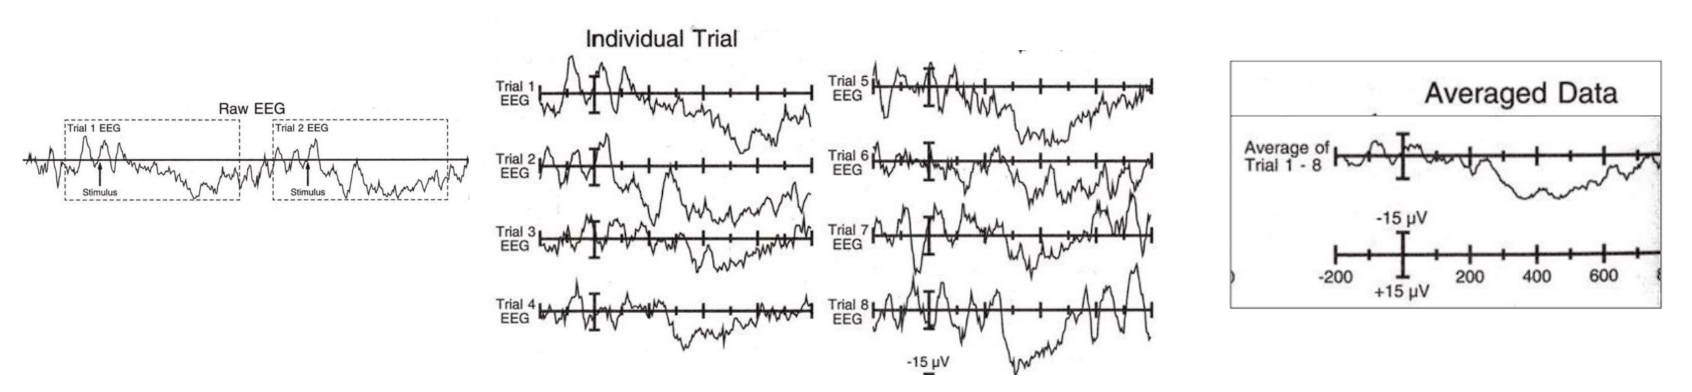
\includegraphics[width=1\textwidth]{images/trials.eps}
     \caption{Averaging different trials of an EEG.}
     \label{AVG_EEG}
\end{figure} 
\subsection{EEG Instrumentation}
The EEG measurements are very tiny (microvolt), the electrodes are sensors that measure these voltages, and are usually made of silver with a surface layer of silver
chloride. Some properties that an electrode should have is\begin{itemize}
    \item nonreactivity to biological tissues
    \item accurate reproduction of extremely slowly changing
potentials
    \item low polarization potentials, drift, and noise.
\end{itemize}
\begin{center}
     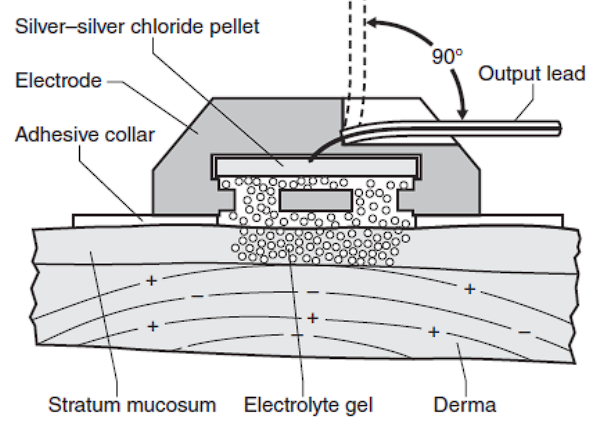
\includegraphics[width=0.4\textwidth]{images/electrode.png}
\end{center} 
The electrode is not directly in contact with the skin, since it needs a uniform surface, so a conductive gel is applied, to create a much more stable interface, and make the skin more conductive.

Neurons communicate by moving charged atoms (ions) such as Sodium ($Na^+$), Potassium ($K^+$), and Chlorine ($Cl^-$) across their membranes.
\begin{itemize}
    \item When a neuron fires, it opens channels that let these ions in or out.
    \item This movement creates a difference in charge between the inside and outside of the cell.
    \item This variation is called Action Potential.
\end{itemize}
Neurons generate streams of ions. These flows create electric fields that propagate in the tissues. The electrode captures the potential variation of these fields and transforms it into an electrical signal, then an analog to digital conversion is applied to display the signal on the screen.\bigskip

Since the potential measured on the scalp is in the order of micro volts, amplifiers are needed to distinguish these signals from the other signals measured by the electrodes that comes from external sources. The simplest type of amplifier is the \textit{operational amplifier}.
\begin{figure}[H] 
     \centering
     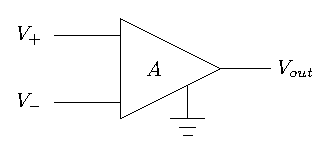
\includegraphics[width=0.2\textwidth]{images/opAmplifier.eps}
     \caption{Schematic of the operational amplifier.}
\end{figure}
The measured potential $V_{out}$ is \begin{equation}
     V_{out}=A(V_+-V_-)
\end{equation}
We need an amplifier that\begin{itemize}
     \item performs an high amplification on the desired signal, without amplifying the noise
     \item have an high input impedance.
\end{itemize}
A real amplifiers can be modeled as follows\begin{equation}
     V_{out}=G_d(V_+-V_-)+G_c\left(\frac{V_++V_-}{2}\right)
\end{equation}
$V_+-V_-$ is the quantity that we want to measure and amplify, and the amplitude of this signal is given by the \textit{differential gain} $G_d$. The \textit{common mode gain} $G_c$ amplifies the common signal that is identical on the two electrodes, and is always gain. In an ideal amplifier, $G_c=0$.
\begin{boxdefinition}{Common-Mode Rejection Ratio}{}
     The \textbf{Common-Mode Rejection Ratio} is the ratio between $G_d$ and $G_c$, it measures how well the amplifier rejects noise that affects both electrodes in the same way (such as 50Hz power line interference) and amplifies only the actual brain signal.
     \begin{equation}
          CMRR=\frac{G_d}{G_c}\Bigg|_{\text{dB}}=20\log_{10}\frac{G_d}{G_c}
     \end{equation}
\end{boxdefinition}
\begin{figure}[H] 
     \centering
     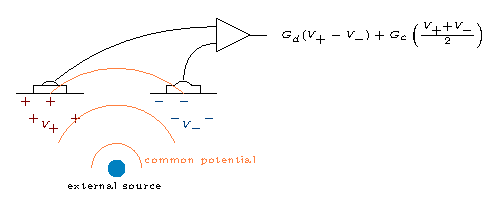
\includegraphics[width=0.7\textwidth]{images/CMRR.eps}
     \caption{The value $\frac{V_++V_-}{2}$ is the common potential shared between the two electrodes.}
\end{figure}
Of course, a good amplifiers should have an high $CMRR$. Due to the huge difference in amplitudes between the signals from the neurons and the signals from the external sources, the differential gain is usually in the order of $10^{15}$ times greater than the common mode gain. Despite this difference, the output of amplifier have still some artifacts to deal with.\bigskip

A desirable feature for an amplifier is an \textit{high input impedance}. Before explaining what the impedance is, we need some electronics concepts, the following circuit is the simplest model of a source and a measurement system.
\begin{figure}[H] 
     \centering
     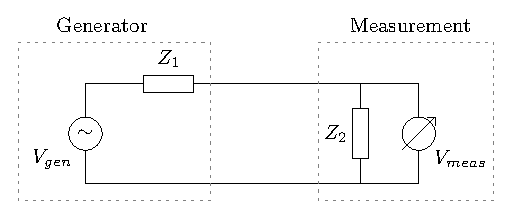
\includegraphics[width=0.6\textwidth]{images/measurement.eps}
     \caption{A simple measurement model.}
     \label{impedance}
\end{figure}
This is a model of  real generator that is an ideal generator in series with an output impedance.\begin{equation}
     V_{meas}=V_{gen}\frac{Z_2}{Z_1+Z_2}
\end{equation} 
The impedance is (in simplistic words) a \textbf{frequency dependant resistance}. The measurement system in Figure \ref{impedance} is a real multimeter, composed by an ideal multimeter (that measures the voltage without disturbing the circuit) plus an impedance in parallel. This is the simplest model of a real measurement system. 

We want the input impedance $Z_2$ to be high, in order to have the most accurate measurement possible:\begin{equation}
     \lim_{Z_2\rightarrow+\infty}V_{gen}\frac{Z_2}{Z_1+Z_2}=V_{gen}.
\end{equation}
For the same argument, we want a low output impedance for the source:\begin{equation}
      \lim_{Z_1\rightarrow 0}V_{gen}\frac{Z_2}{Z_1+Z_2}=\frac{Z_2}{Z_2}V_{gen}=V_{gen}.
\end{equation}
Our output source is the membrane that generates the ionic current, the contact impedance $Z_1$ is given by the pathway that goes from the source (the neurons) to the measurement system (the electrode). Most of the structure in this pathway are low impedance (mostly wet tissues).
\begin{figure}[H] 
     \centering
     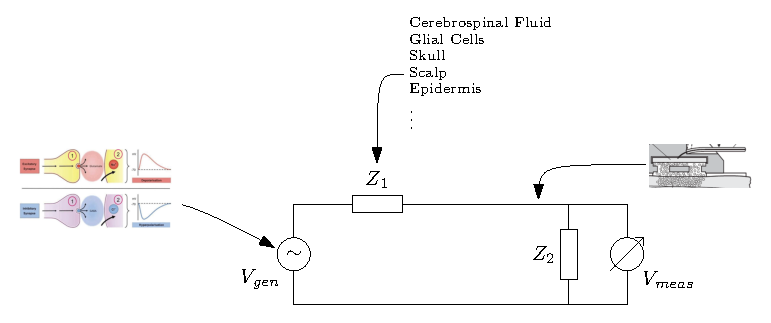
\includegraphics[width=0.7\textwidth]{images/measurement2.eps}
     \caption{A simple measurement model.}
     \label{impedance2}
\end{figure}
The real problem in the impedance is the skin, the surface part of the skin is composed mostly by dead cells, that have an high impedance, for that purpose we use a gel to stabilize the contact surface  and infiltrates the dry skin to moist it, by reducing the impedance.

The international guidelines suggest to keep electrode impedance below 5 k$\Omega$, the modern amplifiers with high input impedance allows to relax this requirement, a typical value for the input impedance is around hundreds of M$\Omega$.
\subsection{Standard Electrode Displacement}
The first standard from the 90's required 19 electrodes.
\begin{figure}[H] 
     \centering
     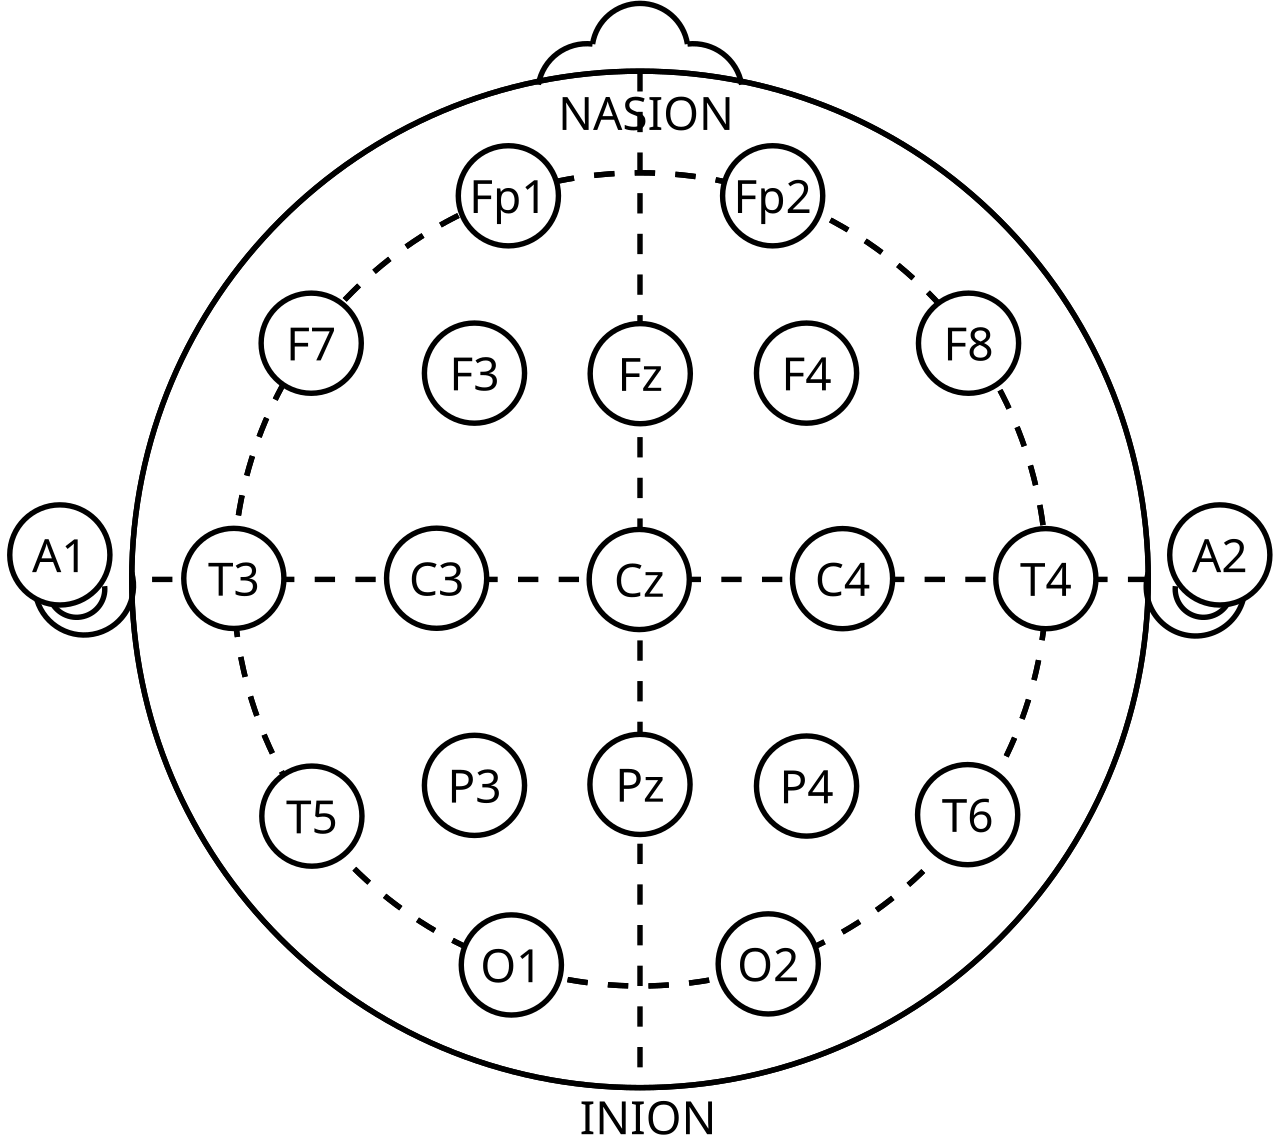
\includegraphics[width=0.35\textwidth]{images/10_20_EEG.png}
     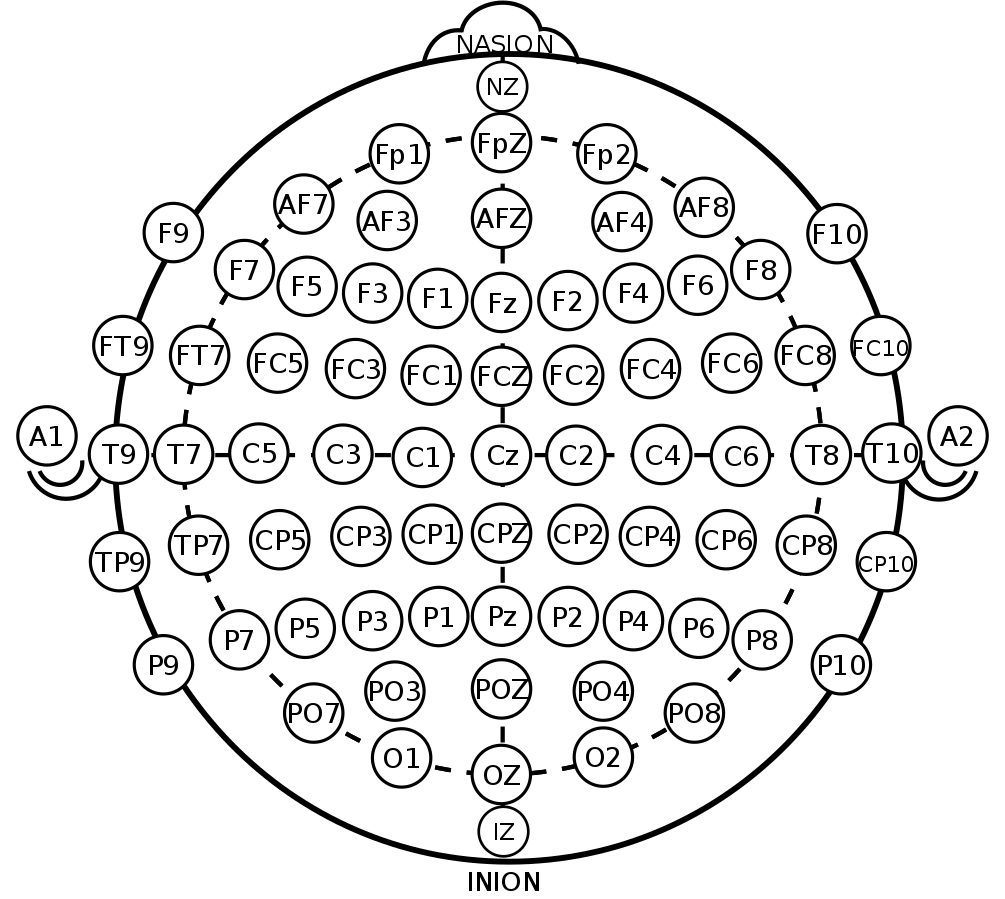
\includegraphics[width=0.35\textwidth]{images/10_10_EEG.png}
     \caption{International 10-20 system (left) and 10-10 system (right) of EEG electrode placement and labeling.}
     \label{10_20_EEG}
\end{figure}
The 10-20 system prescribes where to put the electrodes and what the labels of the electrodes are. For research purposes, 19 electrodes are not enough.Another system is the 10-10 system that uses at most 73 electrodes. The inion and the nasion are points that can be localized on the skull.\begin{center}
     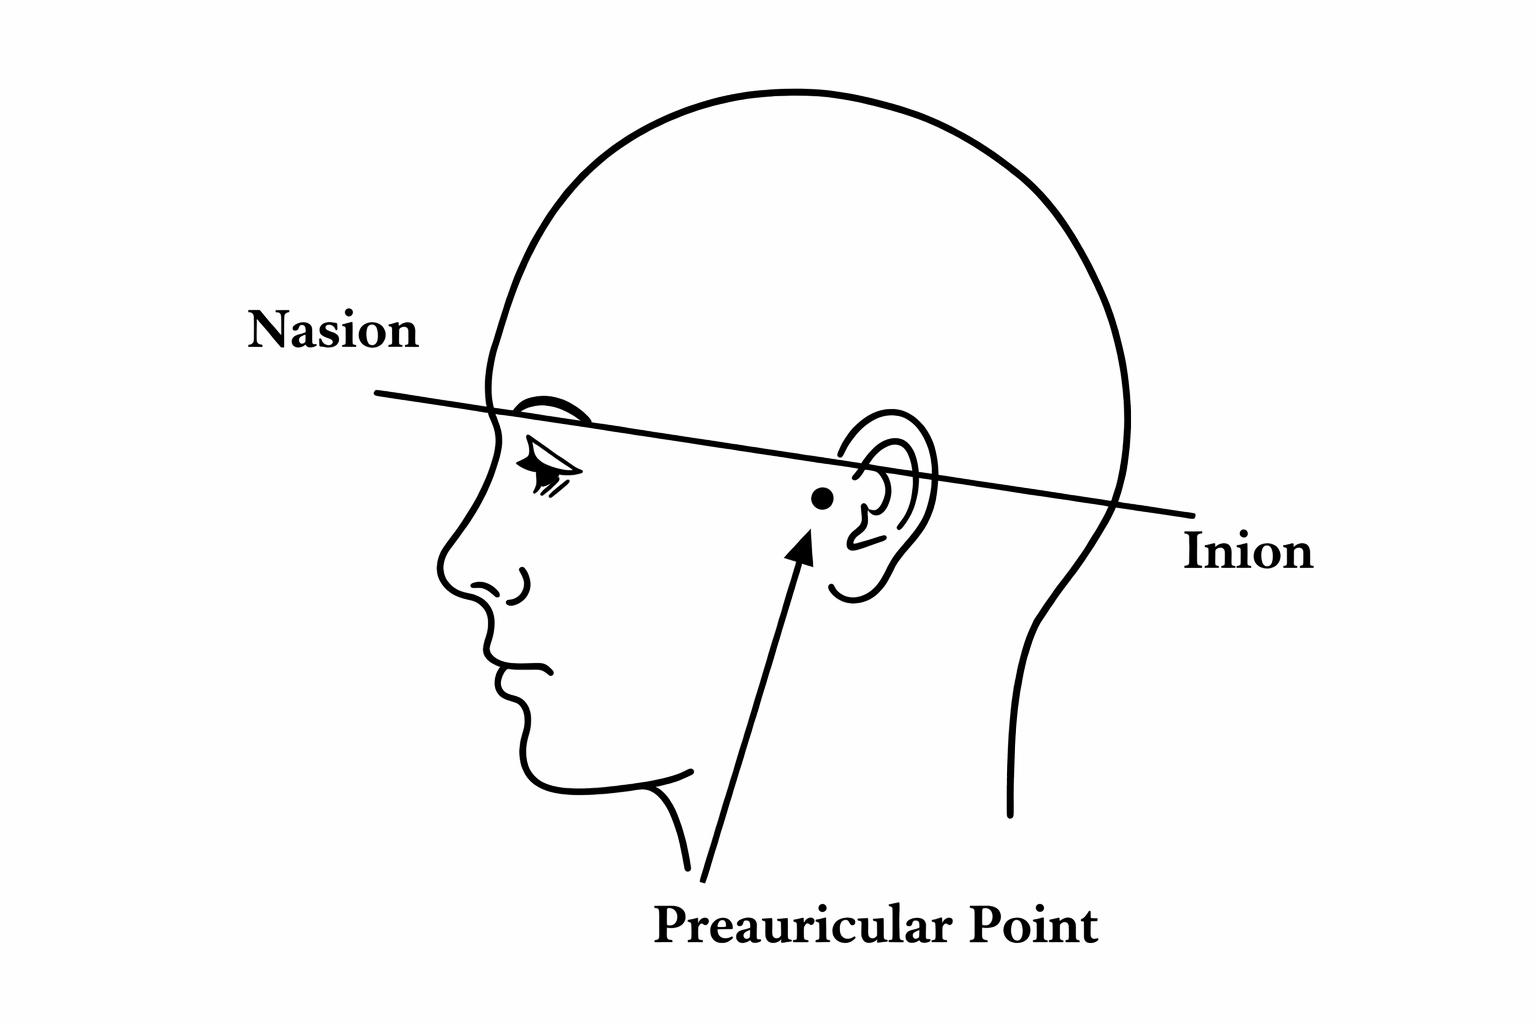
\includegraphics[width=0.5\textwidth]{images/inion_nasion.png}
\end{center}
This points are ''reliable'' and can be located in every skull, allowing to build the standard displacement. The labels on the electrodes (N, AF, F, FT, T, \dots) are named by the lobes of the brain.
\begin{center}
     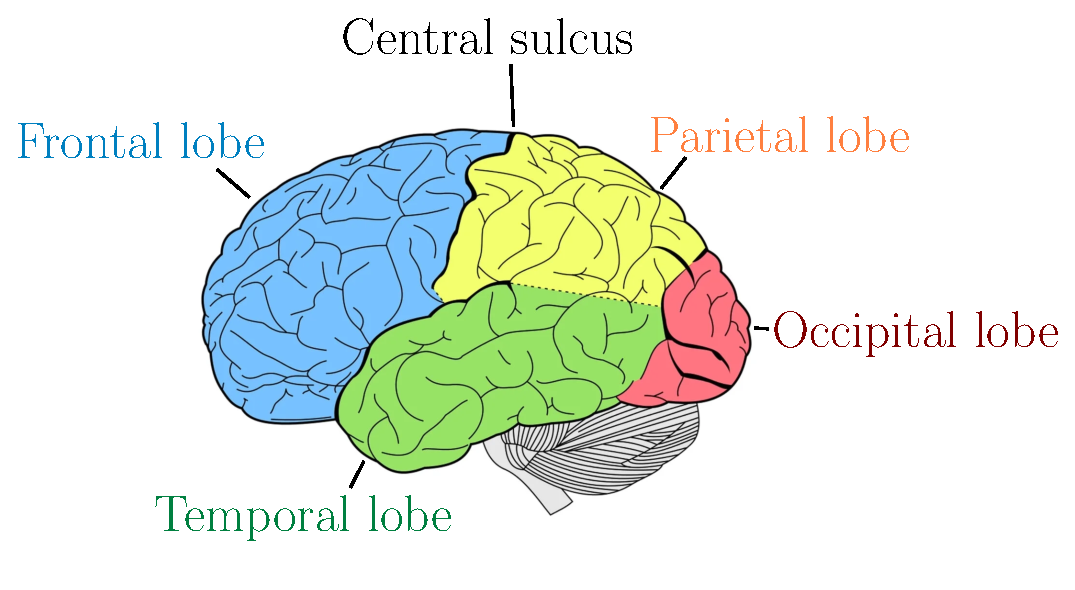
\includegraphics[width=0.6\textwidth]{images/lobes}
\end{center}
There are four lobes, as can be seen in the 10-10 system, the electrodes placed in proximity of the frontal lobes are labeled with an F (or AF), as the labels placed near the temporal and the parietal lobes are labeled with TP. There is an exception for the electrode on the nasion, labeled with N and the electrode on the inion, labeled with I and the ear, labeled with A. 
The electrodes on the left are labeled with an odd number subscript, the labels on the right with an even number, the further the electrodes are from the sagittal arc\footnote{arc connecting the inion and the nasion, that divides the skull in two parts. The electrodes on this segment are labeled with $z$ (zero).}, the greater their number on the label will be.
\subsection{Reference Electrodes}

We define the zero potential as the potential measured at infinite distance (far away from any electrical source). This is a convention, we will have to arbitrary define where is the zero potential. We are measuring the difference of potential so we need at least two electrodes, an additional amplifier is needed for the ground. One of the two electrodes used to measure the difference is called the \textbf{reference electrode}, the other is called \textbf{active electrode}, the reference electrode is placed where we set the potential to zero. So we measure the position of the \textit{active electrode} with reference to the \textit{reference electrode}.

There are no ''good'' position for the reference electrode, but the displacement will influence the signal that will be displayed.

\begin{figure}[H] 
     \centering
     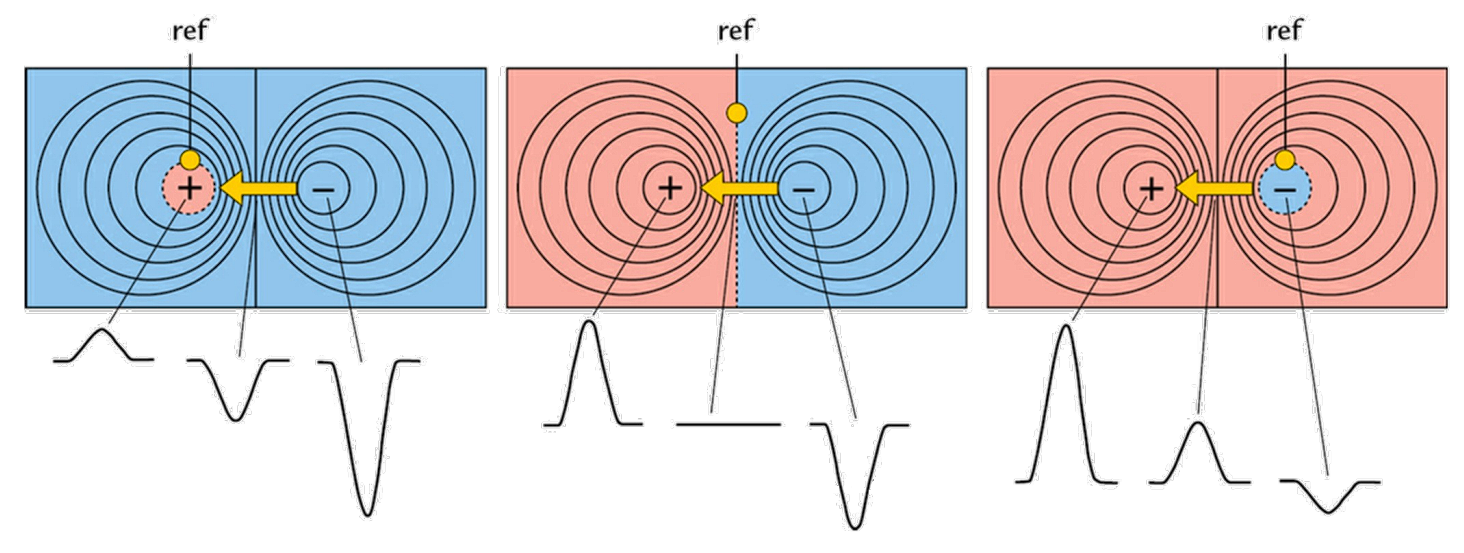
\includegraphics[width=0.7\textwidth]{images/ref_electrodes.png}
\end{figure}

\begin{figure}[H] 
     \centering
     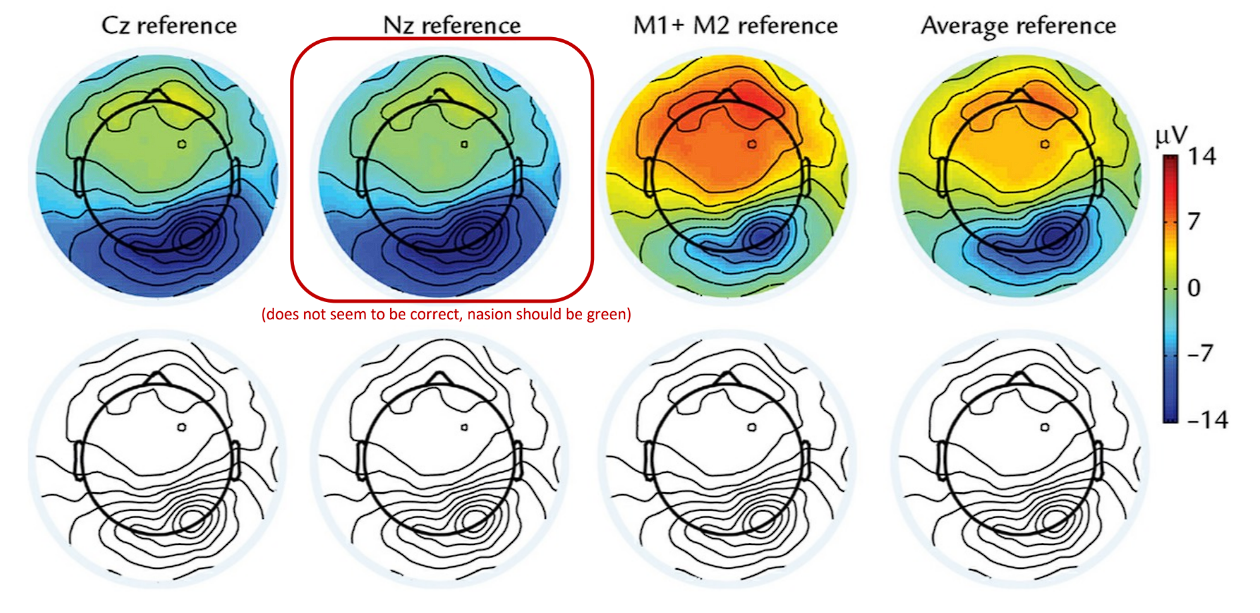
\includegraphics[width=0.7\textwidth]{images/ref_potentials.png}
     \caption{Distributions of potential depending on the reference position. }
\end{figure}

Changing the reference is equivalent to imposing a value of zero on a specific channel. By subtracting the potential of one electrode from all other recordings, that channel becomes the new reference.

While one might attempt to create a paired reference by physically short-circuiting two earlobe electrodes, this is ill-advised. Because potentials are asymmetric across the ears, short-circuiting them forces these two points to an identical potential, which physically redistorts the electric field across the head. 

Instead, this should be handled in software: by recording both electrodes separately, calculating their average, and subtracting it from the remaining channels, we create a mathematically stable \textbf{virtual reference}.


Observe the Figure  \ref{bipolar_monopolar}.
\begin{figure}[H] 
     \centering
     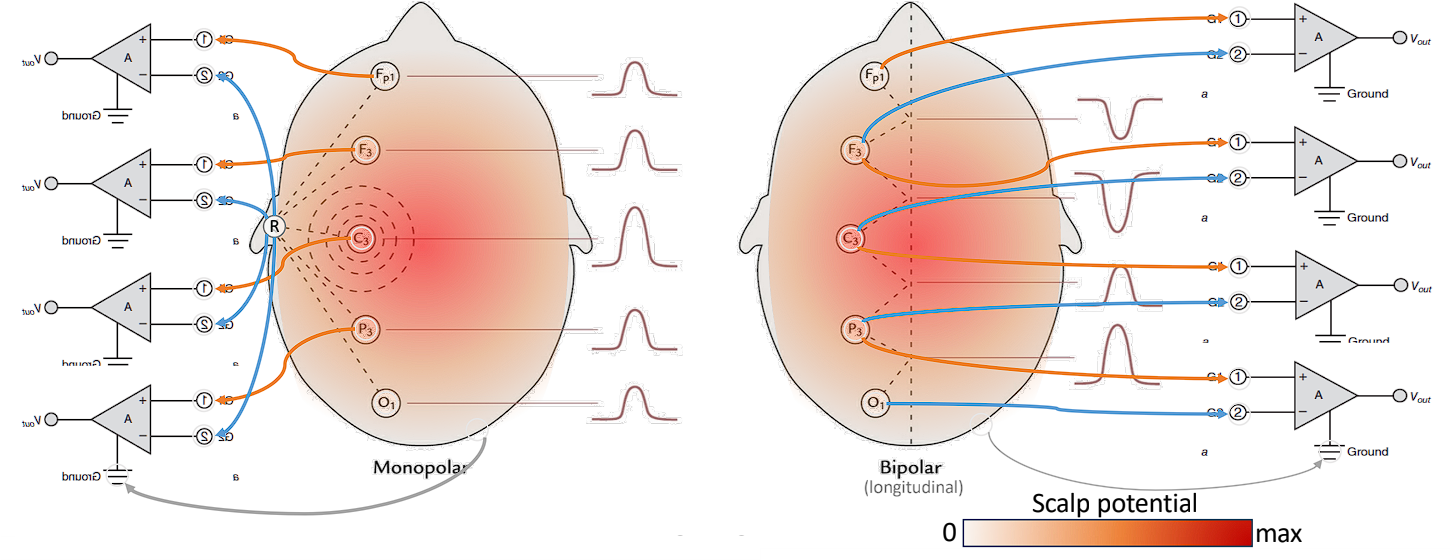
\includegraphics[width=\textwidth]{images/bipolar_monopolar.png}
     \caption{Monopolar vs. bipolar montages}
     \label{bipolar_monopolar}
\end{figure}
\begin{boxdefinition}{}{}
     With \textbf{Montage} we refers to the disposition of electrodes on the skull (displacement and number) and how they are connected.
\end{boxdefinition}
In the left diagram, we are acquiring data from different electrodes by using the same reference electrode, this is a \textbf{Monopolar Montage}: All the channel shares the same potential as a reference.\bigskip

In case of \textbf{Bipolar Montage}, there is not a single reference potential, for each channel to record we use a different reference. Usually, there is a ''line'' of electrodes, and for each channel we use as active electrode, the one that was a reference electrode in the previous channel. In the image, the bipolar montage is placed in a longitudinal way.

As we can observe in the example of figure \ref{bipolar_monopolar}, the potential is distributed in such way to have a peak on the vertex. The monopolar montage in this case mount the reference electrode near the ear where the potential is minimum, and waveform recorded by the channels faithfully represent the potential distribution.

In the bipolar montage the displacement and the connections effects the recording in a different way, for example, the first two electrodes on the top records a negative potential since the reference electrode $F_3$ is closer to the peak, so the difference $F_{p1}-F_3$ is a negative value. The bipolar montage highlight phase reversals, making easier to detect peaks in the potential, so in the clinical practice, the bipolar montage is often used more than the monopolar montage.
\begin{figure}[H] 
     \centering
     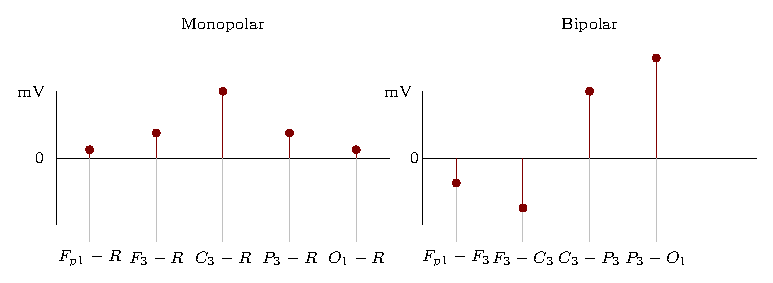
\includegraphics[width=0.7\textwidth]{images/phase_reversal.eps}
     \caption{The phase reversal makes easier to identify the peaks in the potential.}
\end{figure}
\subsection{Data Collection}
Successful EEG experimentation requires meticulous planning and adherence to strict protocols to ensure high-quality, artifact-free data. The following guidelines summarize the key phases of data collection:\bigskip

\noindent\textbf{Planning and Documentation}:
Regardless of whether the experiment is formal or exploratory, rigorous organization is essential:
\begin{itemize}
    \item \textbf{Protocol adherence:} Follow strict experimental protocols at all times.
    \item \textbf{Systematic logging:} Accurately document conditions for every run.
    \item \textbf{Metadata management:} Save explanatory metadata, such as time markers, alongside the primary data for future analysis.
\end{itemize}
\begin{figure}[H] 
     \centering
     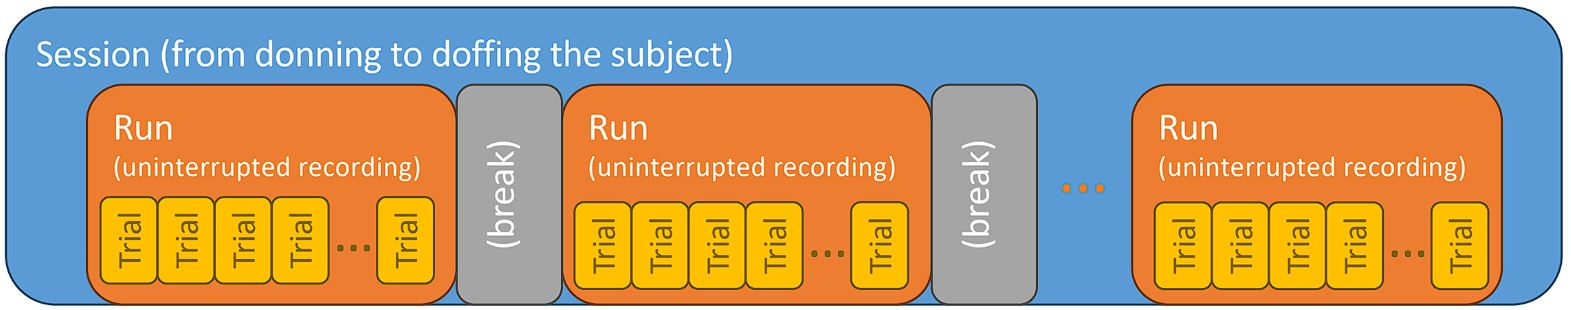
\includegraphics[width=\textwidth]{images/datacollection.png}
\end{figure}

\noindent\textbf{Subject and Electrode Preparation}:
Proper preparation is critical to reducing signal noise and interference:
\begin{itemize}
    \item \textbf{Subject hygiene:} Instruct subjects to wash their hair and skin prior to arrival and avoid cosmetic products.
    \item \textbf{Electrode application:} Utilize conductive gel, applied through the top of the electrode using a blunted needle or syringe.
    \item \textbf{Skin preparation:} Use the blunted needle for light abrasion of the scalp skin when necessary.
    \item \textbf{Impedance targets:} Aim for electrical impedances of less than 5-10 k$\Omega$ to ensure optimal signal quality.
\end{itemize}

\noindent\textbf{Experimental Execution and Monitoring}:
Maintaining the integrity of the data stream during the session:
\begin{itemize}
    \item \textbf{Session structure:} Divide the recording session into smaller, manageable ''runs'' or blocks, interspersed with breaks.
    \item \textbf{Subject comfort:} Consistently remind subjects to relax muscles, minimize eye blinks, and avoid head or body movements to prevent artifacts.
    \item \textbf{Continuous monitoring:} Monitor brain signals online throughout the session to detect and address technical issues or artifacts immediately.
\end{itemize}
\noindent\textbf{\sapText{Author Disclaimer}}: Sections \ref{Artifacts} and \ref{EEGAnalysis}  were not written by me, but by Gioele Migno, taken from the notes at the following link:

\noindent\url{https://github.com/universitymarr/Neuroengineering/blob/master/Notes/Notes_PART_B.pdf}.

\noindent This discussion is valid \underline{exclusively} for these two sections.
\section{Artifacts}\label{Artifacts}
With the term \textbf{artifacts} we refer to external signals that produces electrical activities not related to
the brain. This
activities are recorded together the data and makes it difficult to read EEG data. For that reason in
the first place we have to avoid the generation of artifacts and then remove them from our EEG
recording.
\begin{figure}[H] 
     \centering
     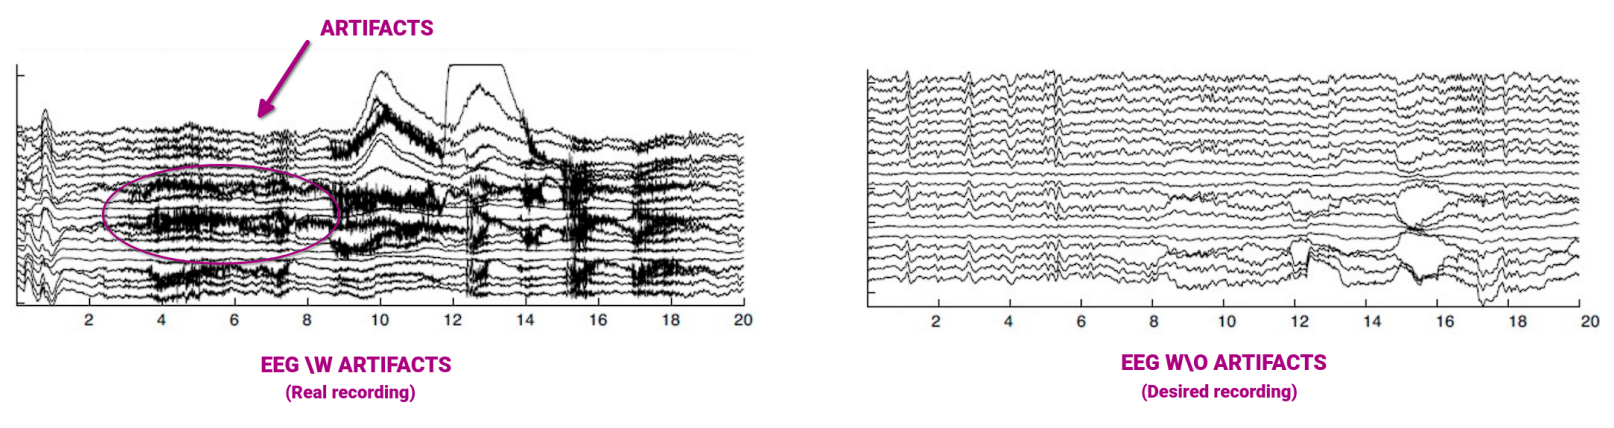
\includegraphics[width=\textwidth]{images/artifacts.png}
\end{figure}
More formally we can define artifact in EEG as any potential difference due to an extracerebral
source. We can distinguish the artifacts of technical and biological origin:\begin{itemize}
     \item Biological: (Physiological) Eye blinks, eye movements (EOG), muscle activity including
swallowing and teeth clenching (EMG), electrocardiogram (ECG).
\item Technical: (Non-Physiological) Power supply, spurious electrical, noise from electrical engines,
bad electrode contact, or its detachment, saturation of the ADC (analog to digital converter)
\end{itemize}
Body and head movements may induce not only muscle electrical activity, but also slow potential
shifts due to the physical displacement of the ions double layer on the electrode surface.\begin{boxobservation}{}{}
     Prevention of artifacts is always preferable to removing or compensating for them post hoc
during data analysis.
\end{boxobservation}
\subsection{Physiological Artifacts}
There are several types of physiological artifacts:\begin{itemize}
     \item Eye-related artifacts
\item Muscle artifacts
\item Cardiac artifacts
\item Sweating artifacts
\end{itemize}
Ocular artifacts arise because the eye is an electrical dipole, with the cornea positively charged with
respect to retina at the back of the eyeball. During eye movements, the eyeball moves within the volume conductor and changes potential
measured on the scalp. Using reference at infinity, we have a positive potential in the direction
pointed by the cornea as shown in the following figure:
\begin{figure}[H] 
     \centering
     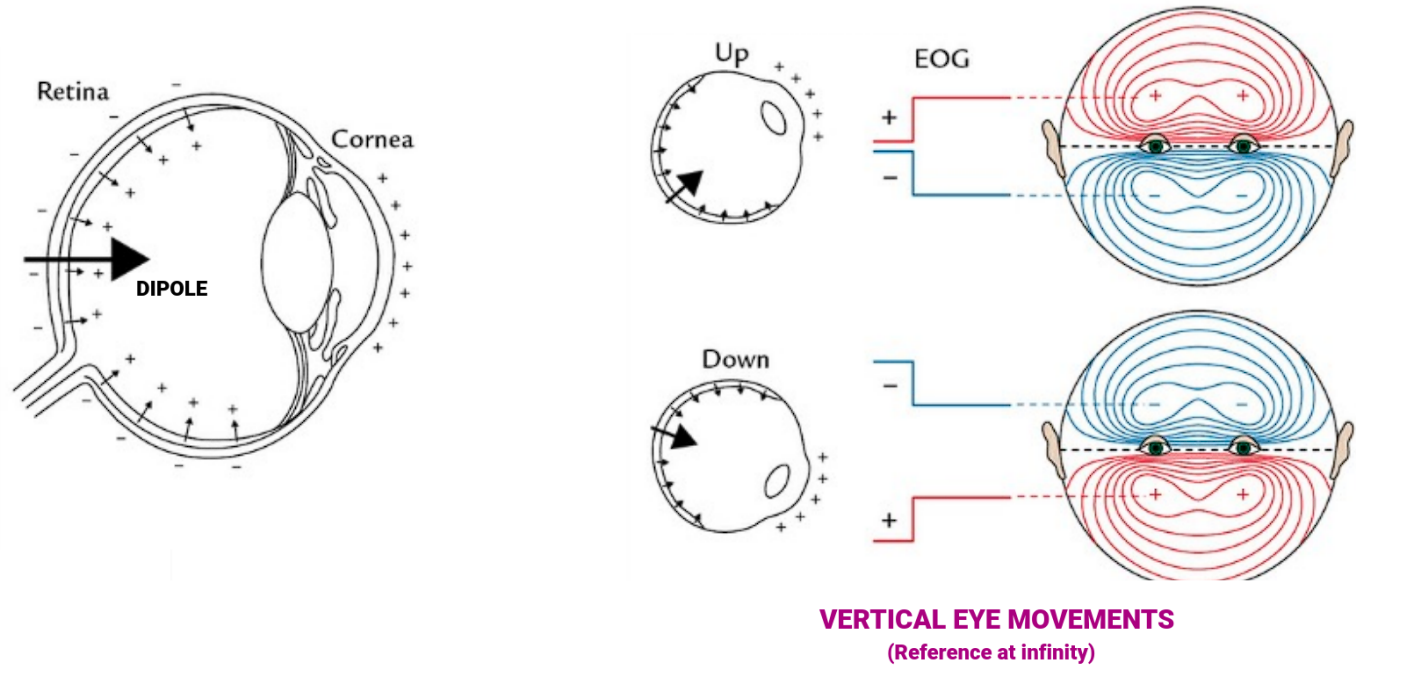
\includegraphics[width=0.7\textwidth]{images/eye_artifacts.png}
\end{figure}
Let's see some example of eye movements artifacts:
\begin{figure}[H] 
     \centering
     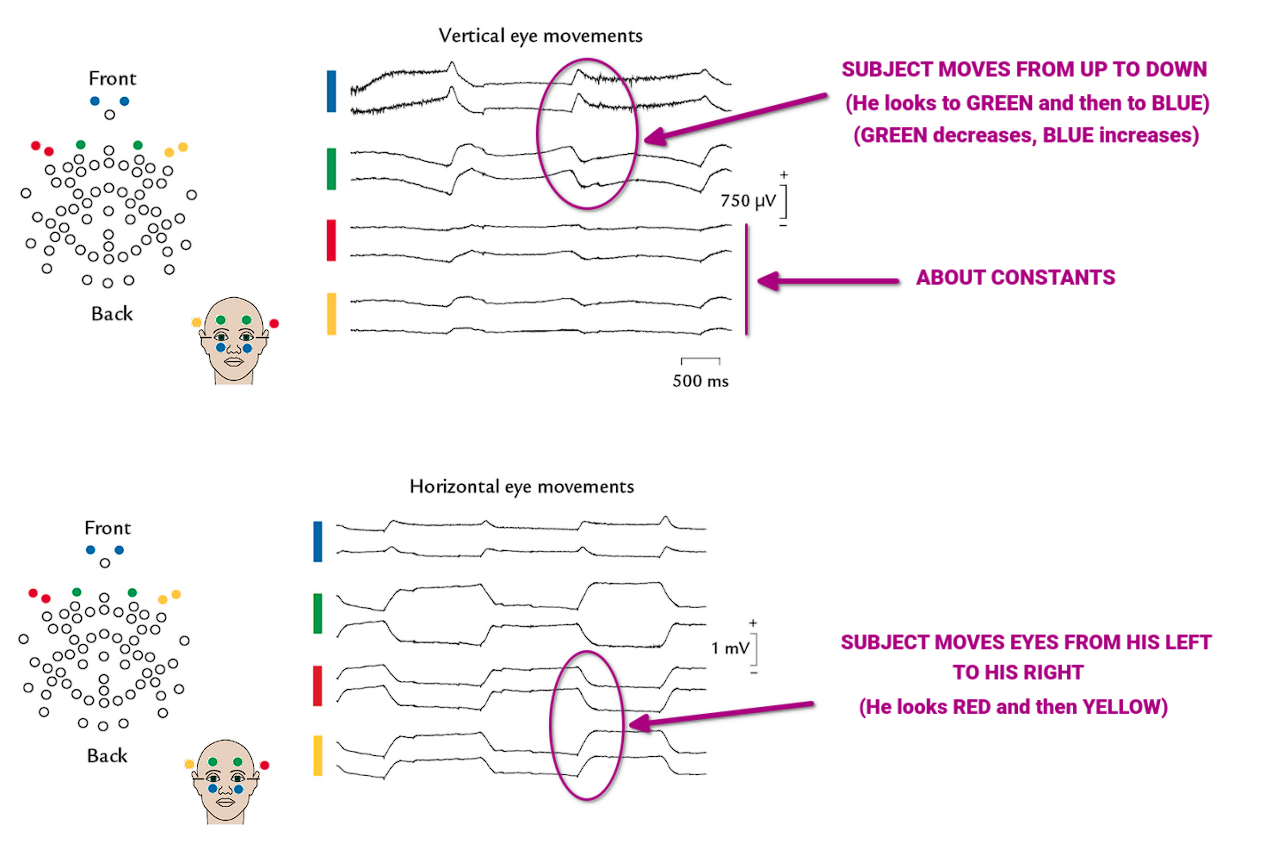
\includegraphics[width=0.7\textwidth]{images/eye_artifacts2.png}
\end{figure}
During \textbf{eye blinks}, the volume conductor changes because of movements of the eyelids that due to
their moist inner surface provide a well-conducting pathway for current flow.
\begin{figure}[H] 
     \centering
     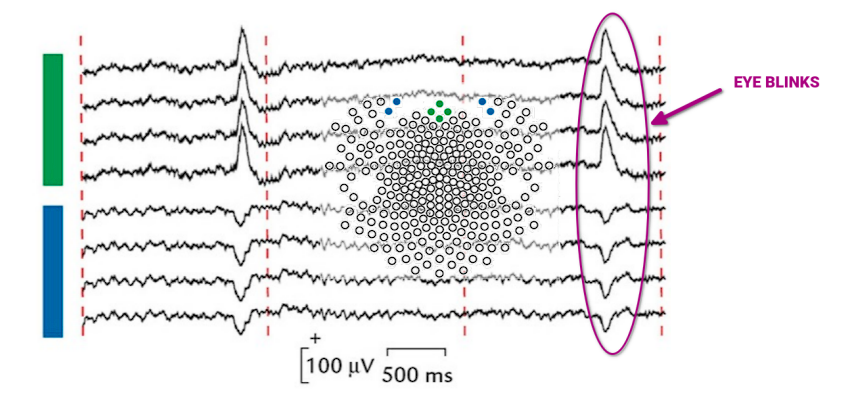
\includegraphics[width=0.6\textwidth]{images/eye_blinks.png}
\end{figure}
These ocular artifacts are of the order of 0.5 mV, monophasic, 200 - 400ms.\bigskip

\noindent\textbf{Muscle Artifacts}: Muscle contractions are seen as artifacts in the 100 $\mu$V or 1 mV range, with a wide frequency
spectrum from tens of Hz to a few kHz, thereby in the same frequency range as beta- and gammaband signals.
The experimenter should always ask the subject to relax the muscles and carefully inspect the EEG
traces to check for contamination. Despite the instructions, subjects may be unable to relax and
release muscle tension.\bigskip 

We distinguish two different types of \textbf{cardiac artifacts}, the first one is not a real issue, let's see both
of them:\begin{itemize}
     \item \textbf{Heart electrical potential}: Electric potentials generated in the heart can be easily recorded, and are known as the
electrocardiogram (ECG). In the literature they can also be referred to by the German-derived
acronym EKG.
In EEG recordings using noncephalic reference electrodes prominent ECG artifacts occur, but less so
when the EEG reference is placed on the subject's head since heart electrical potential is the same
over the head. Therefore, these artifacts usually do not occur during a standard EEG recording.\begin{figure}[H] 
     \centering
     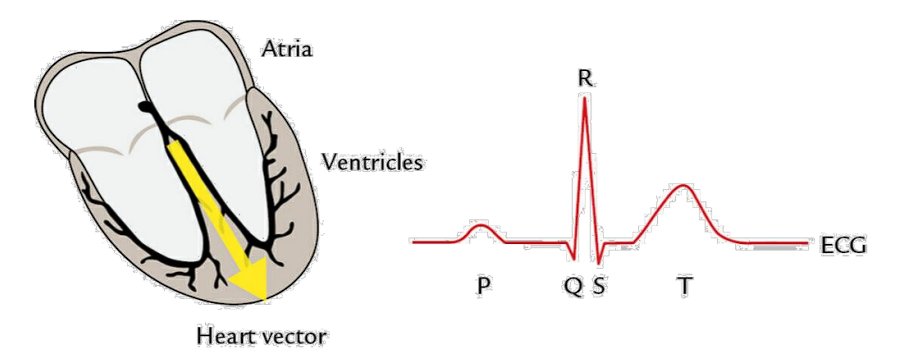
\includegraphics[width=0.5\textwidth]{images/cardiac1.png}
\end{figure}
     \item \textbf{Ballistocardiogram}: Another important cardiac-cycle-related artifact in EEG data results from the ballistocardiogram that
reflects small electrode movements due to a nearby blood vessel in the scalp. This artifact is usually
clearly visible during online monitoring, and it can be eliminated by moving the EEG electrode a small
distance.\begin{figure}[H] 
     \centering
     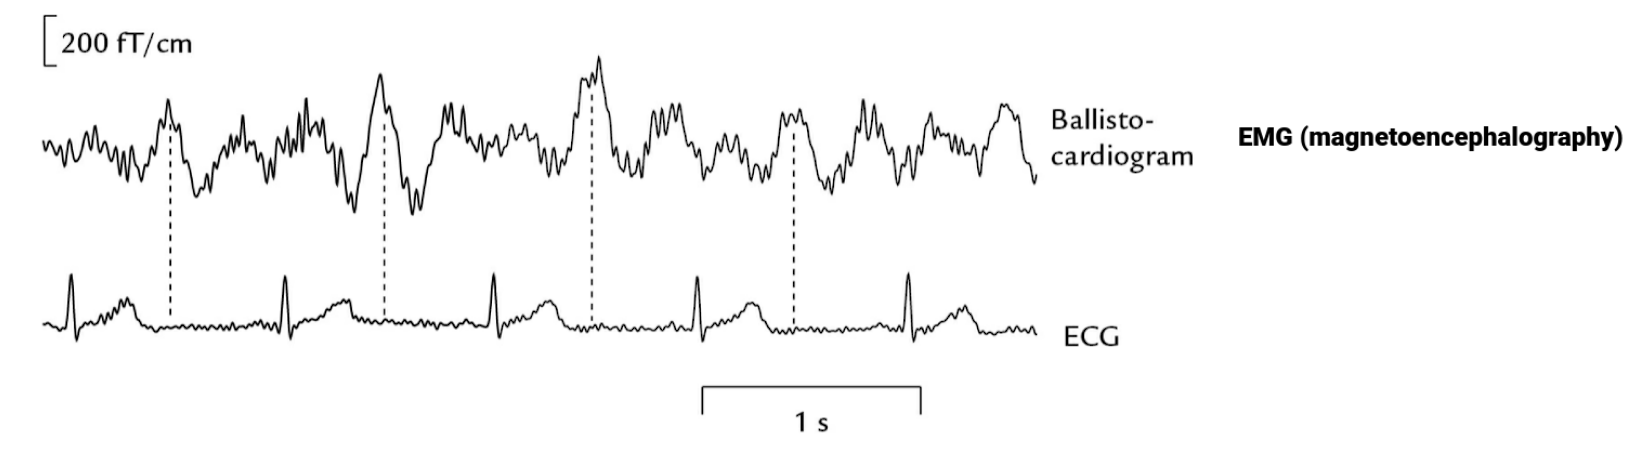
\includegraphics[width=0.6\textwidth]{images/cardiac2.png}
\end{figure}
\end{itemize}
\textbf{Sweating} can be a problem in EEG recordings as it is accompanied by electrodermal responses,
high-amplitude slow ($<$ 0.5 Hz) potentials.
\subsection{Non-Physiological Artifacts}There are several types of non-physiological artifacts: powerline artifacts, electrode-related artifacts and motion artifacts.\bigskip

\noindent \textbf{Powerline artifacts}: Power-line noise arises from the capacitive coupling of alternating current supplied to electrical wall
outlets, thIs line noise occurs either at 50 Hz (or 60 Hz) and at their harmonics, thus, in the time
domain, the signal is not necessarily a sinewave. Powerline artifacts are accentuated in EEG
electrode pairs that have an impedance mismatch (reduced CMRR). Unless there are no other
alternatives, a digital notch filter set to the appropriate line frequency (and its harmonics, if
necessary) can remove this noise.
\begin{figure}[H] 
     \centering
     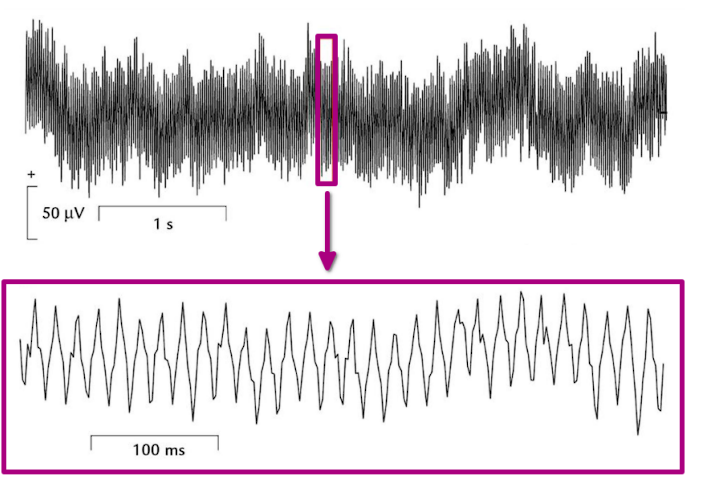
\includegraphics[width=0.5\textwidth]{images/powerline.png}
\end{figure}
\noindent \textbf{Electrode-related artifacts}:
A number of different artifacts can arise from improperly applied EEG electrodes:\begin{itemize}
     \item 
     Bad electrode: artifacts as very slow baseline drifts
      \item  Electrode pop: is an intermittent phenomenon that appears as a sharp, sudden rise followed by a
     gradual fall in the EEG signal of a single electrode. It can happen due to an accumulation of
     capacity in an electrode
\end{itemize}
\begin{figure}[H] 
     \centering
     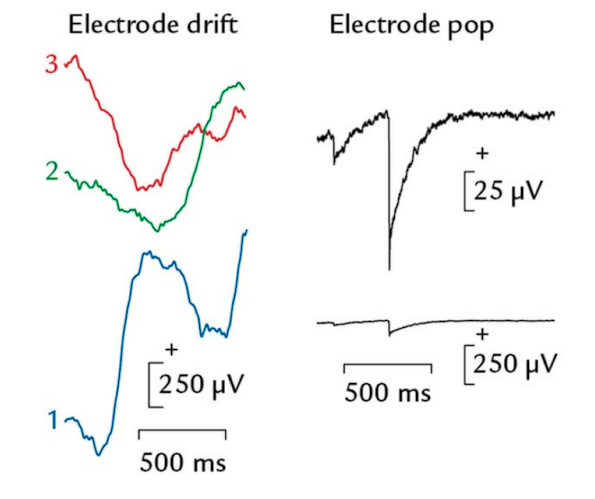
\includegraphics[width=0.35\textwidth]{images/bad_electrodes.png}
\end{figure}
Regarding to electrode drift, sometimes it can happen that all your channels are good but there are 1
or 2 channel that are behaving differently. It means that you see something like sweating, and you
see that one electrode is going up and down like 1, or 2 and 3.
In EEG recordings, artifacts can be created by the experimenter's movements around the subject,
and this problem can be exaggerated in dry air environment creating a problem with static electricity.\bigskip

\noindent \textbf{Motion Artifacts}: At the interface between metal (electrode) and ionic conductor (gel/skin) there is a displacement of
ions that resembles a capacitor. Movement of the electrode (e.g. produced by movements of the
subject's head) disturbs the geometry of the ''capacitor'', producing a relatively strong potential.
\section{EEG Analysis}\label{EEGAnalysis}
In this section we will see some very basic EEG data analysis techniques.\bigskip

\textbf{Off-line data inspection}:
The first step before any kind of analysis is to perform a (off-line) data inspection, namely review
raw data before processing and analysis. Bad EEG segments or channels must be removed from the
data, in this step is important to understand which artifacts mostly affect the results of the analysis,
so that we do not waste data by rejecting too much of it. From a practical point of view, dealing with
bad channels or epochs will depend on the analysis software we are using.\bigskip

EEG data are typically collected in experiments using multiple trials per condition, as the signals of
interest may be quite small, but one of the basic assumptions of analysis is that the signal remains
the same during the whole experiment although it is masked by noise.
With the term \textbf{evoked potential} (EP) we indicate the stimulus-driven activity. In contrast, the terms
event-related potential (ERP) is used more generally to describe changes in EEG signals triggered by
either external stimuli or related to internal mental or task-related events.
\begin{boxobservation}{}{}
     A stimulus can be also produced by the subject, for example when he moves a finger. So in
general we can distinguish two different classes of stimulus:\begin{itemize}
     \item External Stimulus: External stimulus independent by the subject.
  \item Internal Stimulus: Interval stimulus caused by the subject.
\end{itemize}
\end{boxobservation}
\noindent We will see two different kind of EEG analysis:\begin{itemize}
     \item Analysis EP EEG: (EP = Evoked Potential) Analysis of an EEG recording during external
stimulation.
 \item  Analysis Spontaneous EEG: Analysis of an EEG recording without external stimulation.
\end{itemize}
\subsection{Analysis of EP EEG}
About the first type of EEG analysis, we see only (synchronized) averaging that we have already
briefly introduced in previous sections. The continuous EEG record must first be ''cut up'' into epochs (or segments)—consisting of a prestimulus or a pre-event period, followed by a period of time suitably long enough to be able to
highlight the particular activity of interest.\bigskip

\textbf{Averaging}: Signal averaging is based on the assumption that the recorded time-varying signal $x(t)$ comprises a
distinct signal embedded in noise. Averaging $N$ responses would improve the signal-to-noise ratio by
$\sqrt{N}$, namely noise amplitude decreases as $\frac{1}{\sqrt{N}}$ where $N$ is the number of trials.
\begin{figure}[H] 
     \centering
     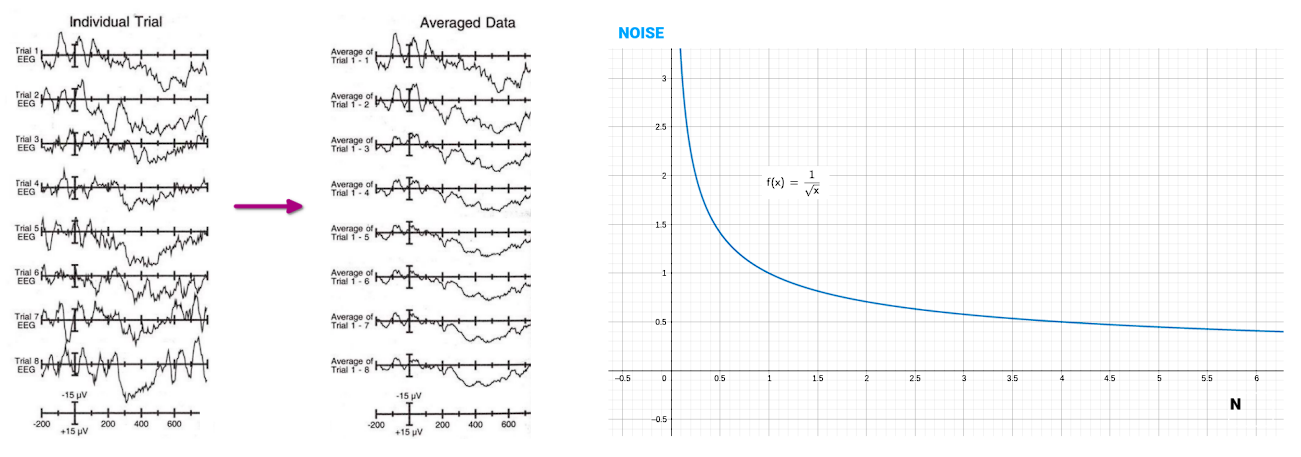
\includegraphics[width=0.8\textwidth]{images/noise_reduction.png}
\end{figure}
\textbf{ERP components}:The peak amplitudes (with respect to pre-stimulus baseline) and latency (with respect to stimulus
onset, or relative to a motor event) are commonly measured.
\begin{figure}[H] 
     \centering
     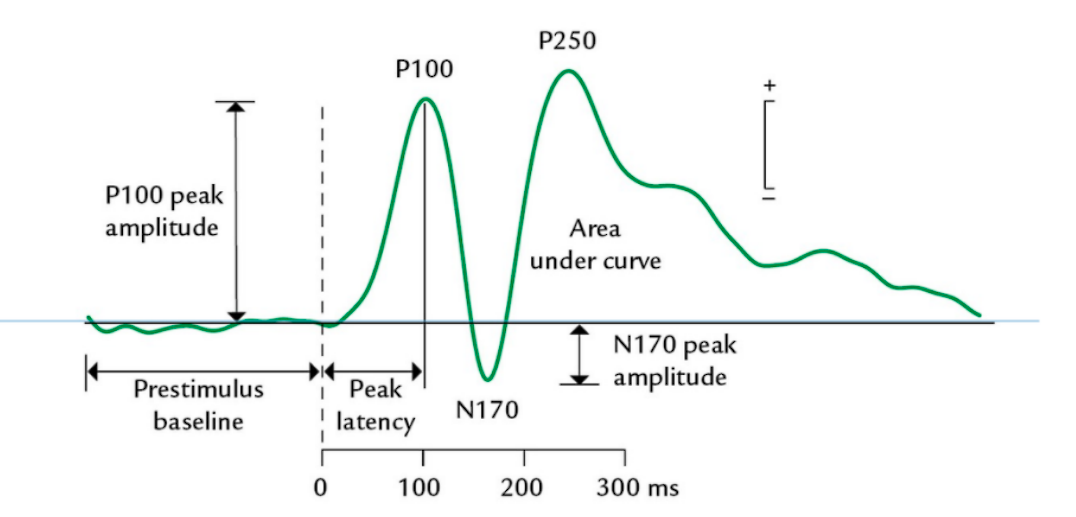
\includegraphics[width=0.7\textwidth]{images/ERP.png}
\end{figure}
In the vast EEG and MEG literature, the nomenclature of evoked responses is diverse and confusing.
An old naming convention numbered successive deflections separately for scalp-positive (P) and
scalp-negative (N) EPs—where the polarities refer to the ''active electrode''—resulting in notations
such as P1, N1, P2, N2, P3. To make matters worse, letters are sometimes added to these labels,
such as P3a and P3b.
A less ambiguous way is to combine the polarity (N or P) of the response peak or trough with the
nominal peak latency in milliseconds, for example, P60, N100, and P200.\begin{boxobservation}{Nominal Latency}{}
     Note that in most cases it is clear enough to use in the response name the approximate (or
nominal) latency (and not the measured individual latency). For example, the mean peak
latency of the N100 deflection may vary between, say, 90 or 110 ms without causing any
confusion in the nomenclature.
\end{boxobservation}
\noindent Let's see some \textbf{standard time quantities}:\begin{itemize}
     \item Stimulus Onset Asynchrony (SOA): Refers to the time between two successive stimulus onsets.
     \item Interstimulus interval (ISI): Refers to the time between the offset of one stimulus and the onset
of another.
     \item Intertrial interval (ITI): Refers to the time between the beginning of subsequent trials (during
which multiple stimuli may be presented).
\end{itemize}
\begin{figure}[H] 
     \centering
     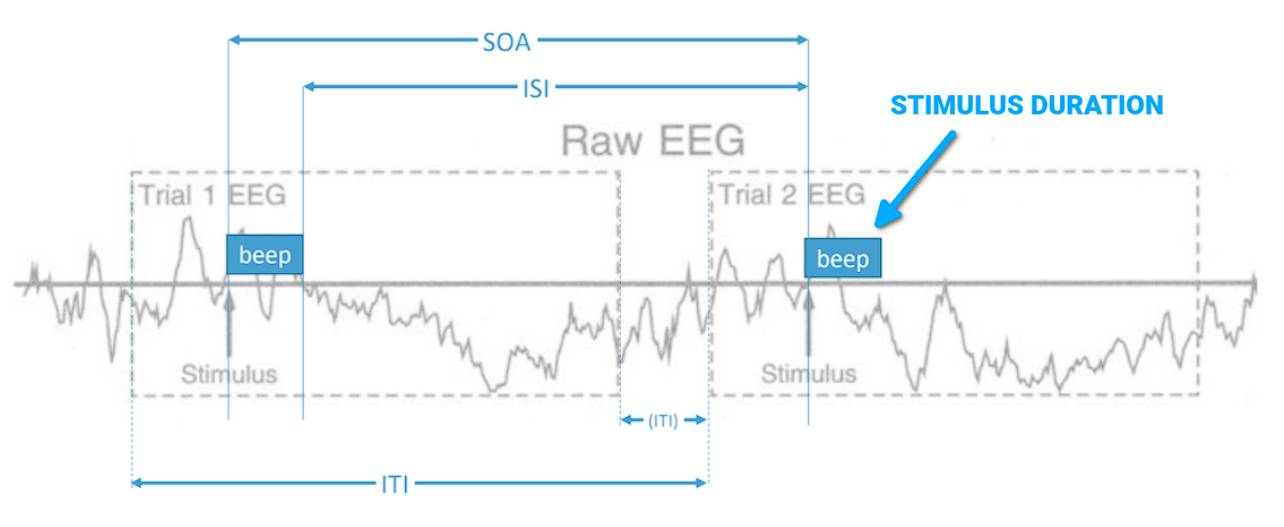
\includegraphics[width=0.7\textwidth]{images/time_quantities.png}
\end{figure}
\begin{boxobservation}{Long Stimulus Duration}
     SOA and ISI/ITI can be quite different from each other if the stimulus duration is long,
indeed we have:\begin{equation}
     \text{ISI}=(\text{SOA$-$stimulus duration}).
\end{equation}
\end{boxobservation}
\noindent\textbf{Effect of stimulus timing}:The shape and amplitude of the ERP may strongly depend on the timing of stimuli. In general, the
longer the latency of the response, the more sensitive the response is to stimulus repetition rate,
namely brain tends to respond less stronger to the same stimulus repeated several times in a short
interval. Therefore, since we want to reduce the overall time of the EEG recording we have a tradeoff
between number of stimuli (noise decreases in $N$) and SOA (total time = $N\cdot$SOA).
\begin{figure}[H] 
     \centering
     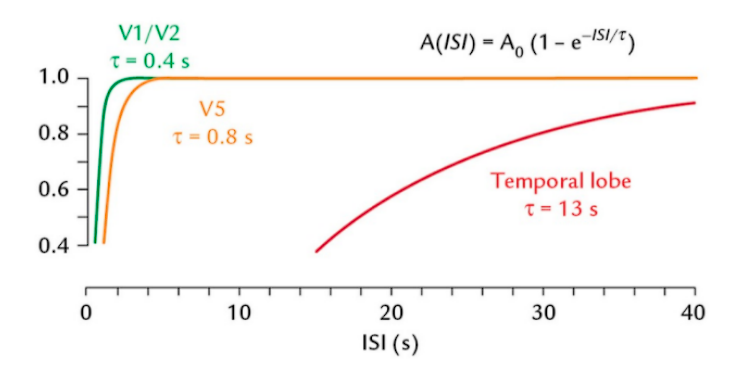
\includegraphics[width=0.6\textwidth]{images/stimulusTiming.png}
\end{figure}
\subsection{Analysis of Spontaneous EEG}
The second type of EEG analysis that we see is analysis of spontaneous EEG where we are
interested to study EEG response after a internal stimulus namely a stimulus produced by the
subject (e.g. finger movement or mental task).\bigskip


The first huge different between external and internal stimulation is that in the last one, response
time of subject can vary, namely time between stimulus delivery and EEG signal response is not
always the same (non-phase response). This time quantity is called jitter.
Spontaneous or ongoing brain activity is always present irrespective of whether or not a subject
performs a task, and it can influence how evoked and induced responses evolve and how they are
related to perception and cognition.\bigskip


We have seen in previous EEG analysis, where the evoked activity is time-locked (phase-locked) to
the stimulus, that EEG stimulus response can be uncovered by stimulus-locked averaging
(synchronized averaging). However, this technique cannot be applied easily in this case due to jitter.\bigskip


Let's compare phase-locked response and non-phase locked EEG responses assuming their shapes
are the same at each trial.
\begin{figure}[H] 
     \centering
     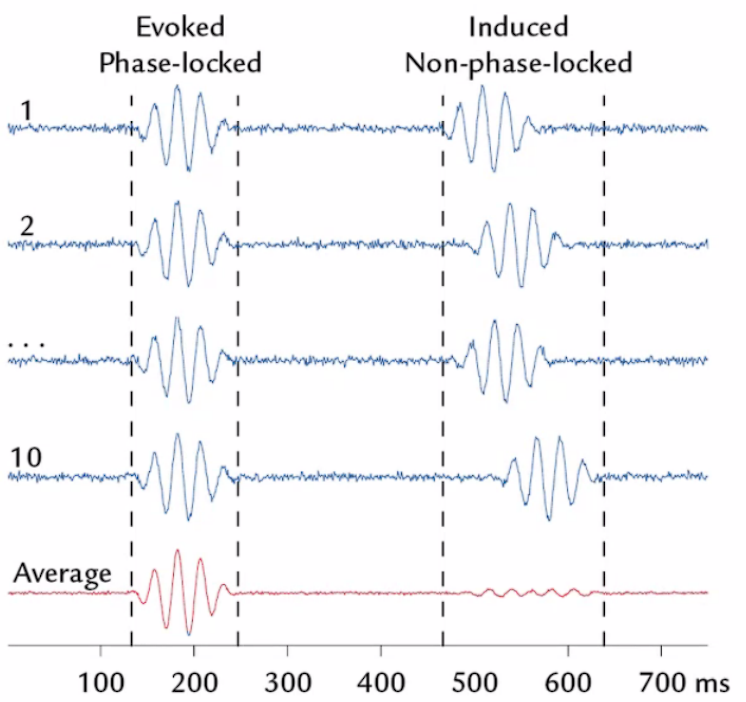
\includegraphics[width=0.4\textwidth]{images/evoked_induced.png}
\end{figure}
As we can see from the previous figure (EEG non realistic), averaging non-phase-locked responses
provided a resulting zero response that will be lost for sure behind ongoing EEG activity. To perform
averaging properly we should align the response of each trial, this method is not so easy in practice
and can be considered as an advanced technique.
A more simple technique to averaging non-phase-locked responses is to use compute the average
envelop, doing that the final average will not be zero since each envelop is always positive:
\begin{figure}[H] 
     \centering
     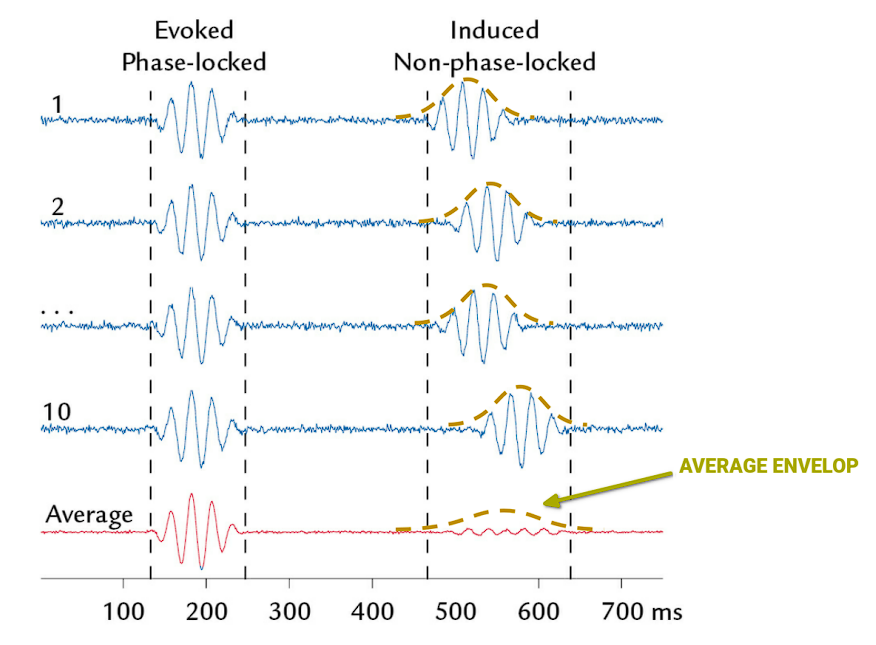
\includegraphics[width=0.5\textwidth]{images/evoked_induced2.png}
\end{figure}
Let's now see how this technique is applied in real scenarios where we call a negative envelop \textbf{event
related desynchronization (ERD)} and a positive envelop \textbf{event related synchronization (ERS)}.\bigskip

\noindent\textbf{Event related desynchronization/synchronization (ERD/ERS)}:  Let's define more clearly these two quantities:

\begin{itemize}
    \item \textbf{Event Related Desynchronization (ERD):} \textit{Negative} variation of the EEG power rhythms at one time relative to a \textit{baseline} period at another time.
    \item \textbf{Event Related Synchronization (ERS):} \textit{Positive} variation of the EEG power rhythms at one time relative to a \textit{baseline} period at another time.
\end{itemize}

The steps to follow to obtain these quantities from $N$ raw EEG trials are the following:

\begin{enumerate}
    \item \textbf{Bandpass filtering} of all event-related trials.
    \item \textbf{Squaring} of the amplitude samples to obtain power samples.
    \item \textbf{Averaging of power samples} across all trials.
    \item \textbf{Averaging over time samples} to smooth the data and reduce the variability.
\end{enumerate}
\noindent At the end the result is expressed as percentage variation of the signal respect to the baseline.

In the following figure one example for each type of envelop is shown: one example of dominant ERD in the alpha band on the left side and one example with dominant ERS in the beta band on the right side.
\begin{figure}[H] 
     \centering
     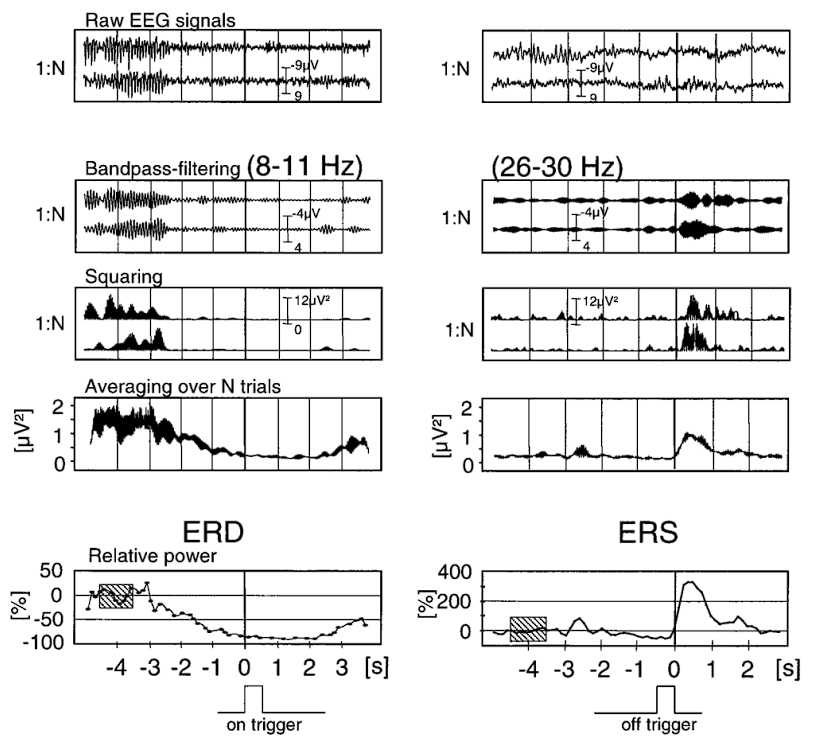
\includegraphics[width=0.5\textwidth]{images/ERD_ERS.png}
\end{figure}
In the case of ERD we are interested into mu rhythmic, indeed the stimulus correspond to a finger
movement by the subject.
\begin{boxobservation}{Large Time Window}{}
     As we can see from the previous figure, it is necessary to start EEG signal recording several
seconds before the stimulus, this is necessary to detect the baseline signal. Baseline is
''faraway'' because the subject's brain prepares in advance to move the finger, indeed this is
a voluntary movement.
\end{boxobservation}
\section{Time Frequency EEG Analysis}
\textbf{Time-frequency analyses} go one step further by computing and visualizing the spectral or amplitude content of the signal as a function of time simultaneously for all frequencies of interest. Fourier transforms, Hilbert transforms, and wavelet-based approaches can be used to calculate MEG/EEG signal power (amplitude). Using this procedure, features in MEG/EEG data can be visualized in both time and frequency.

The following figures show examples of time-frequency plots, in particular they show the frequency of EEG signals during a visual task with two conditions: a face gazing away (Eyes away) and at the subject (Eyes direct) as a function of time. Vertical color scale indicates power in dB. The two conditions show very similar profiles of activity: a prolonged increase in theta and alpha activity and a prolonged decrease in beta activity after the stimulus (vertical broken line). Passband 0.1-200 Hz. Data are from a nine-electrode cluster centered on the left sensorimotor scalp.
\begin{figure}[H] 
     \centering
     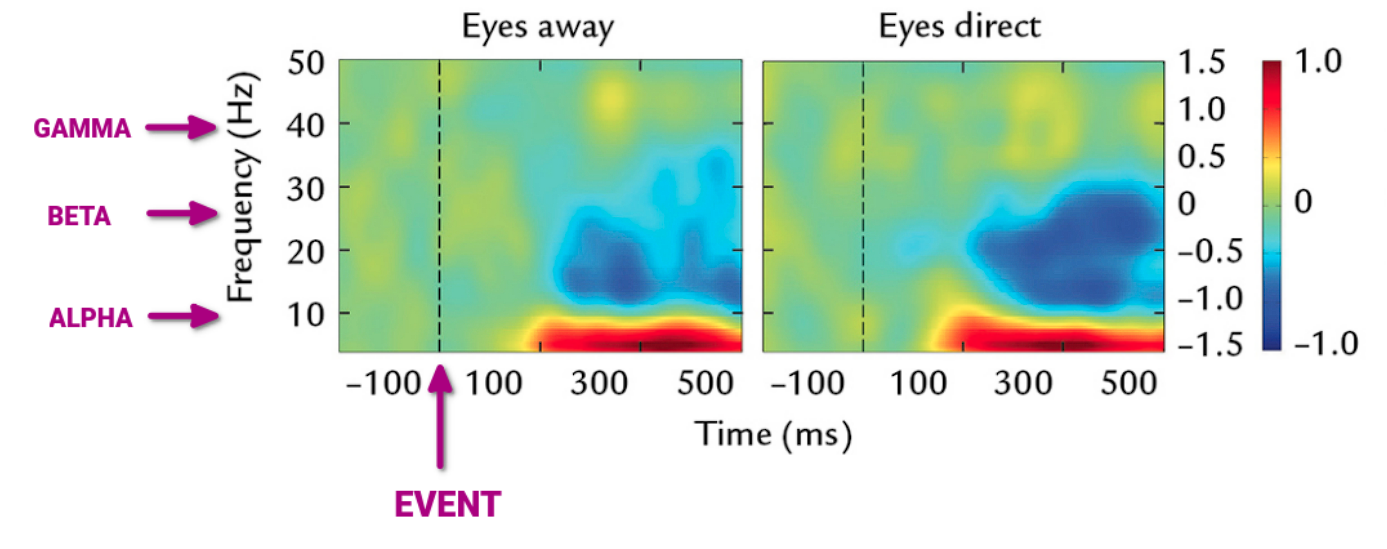
\includegraphics[width=0.5\textwidth]{images/tf_EEG.png}
\end{figure}
One important concept is \textbf{resolution tradeoff}: Improving time resolution worsens spectral resolution (and vice versa).
\begin{figure}[H] 
     \centering
     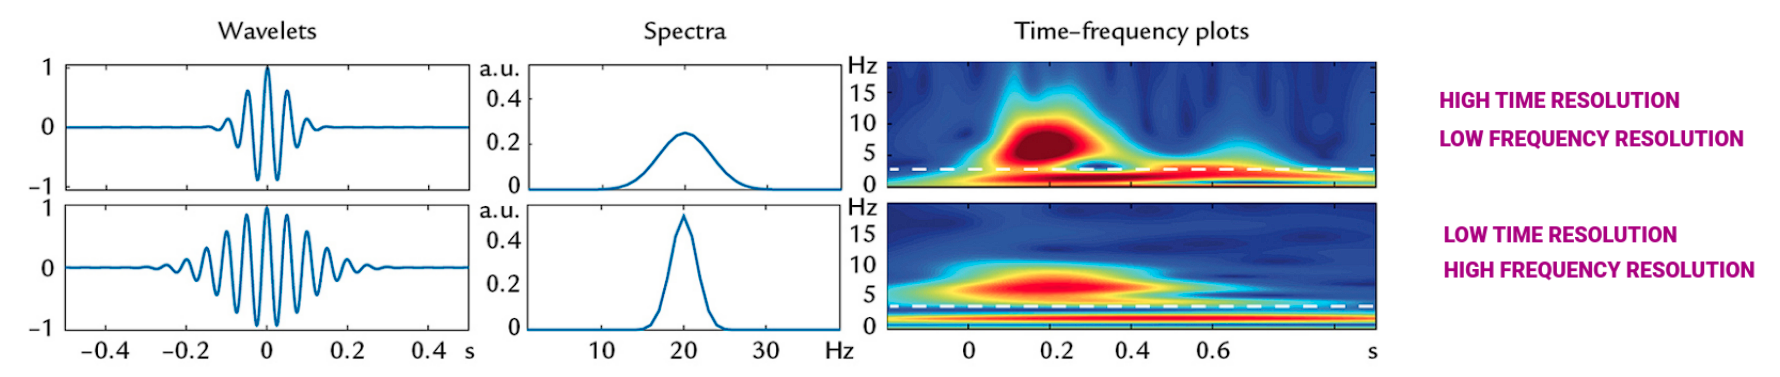
\includegraphics[width=\textwidth]{images/res_tradeoff.png}
\end{figure}
\chapter{Signal Processing}\label{sig_proc}
This section is a small recap of some basic signal processing concepts.
The bio-signal processing procedure follows a precise pipeline:\begin{enumerate}
     \item the bio signal (as electrical energy generated by ionic current) is perceived by a transducer
     \item there is an amplifier that makes the signal readable 
     \item the analog signal is converted into a digital signal 
     \item the digital signal is stored in a buffer and processed by a computer 
     \item the processed signal is displayed.
\end{enumerate}
\begin{figure}[H] 
     \centering
     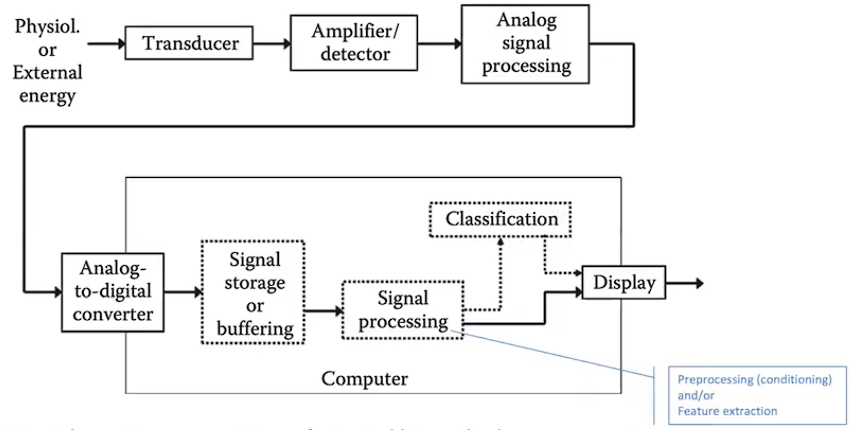
\includegraphics[width=0.7\textwidth]{images/sig_processing.png}
\end{figure}
\section{Sampling and Quantization}
The signal processed by the bio signal aplifier is a continous signal in the time domain and in the amplitude domain, we need to digitalize the signal by discretizing the time (sampling) and amplitude axis (quantization).
\begin{figure}[H] 
     \centering
     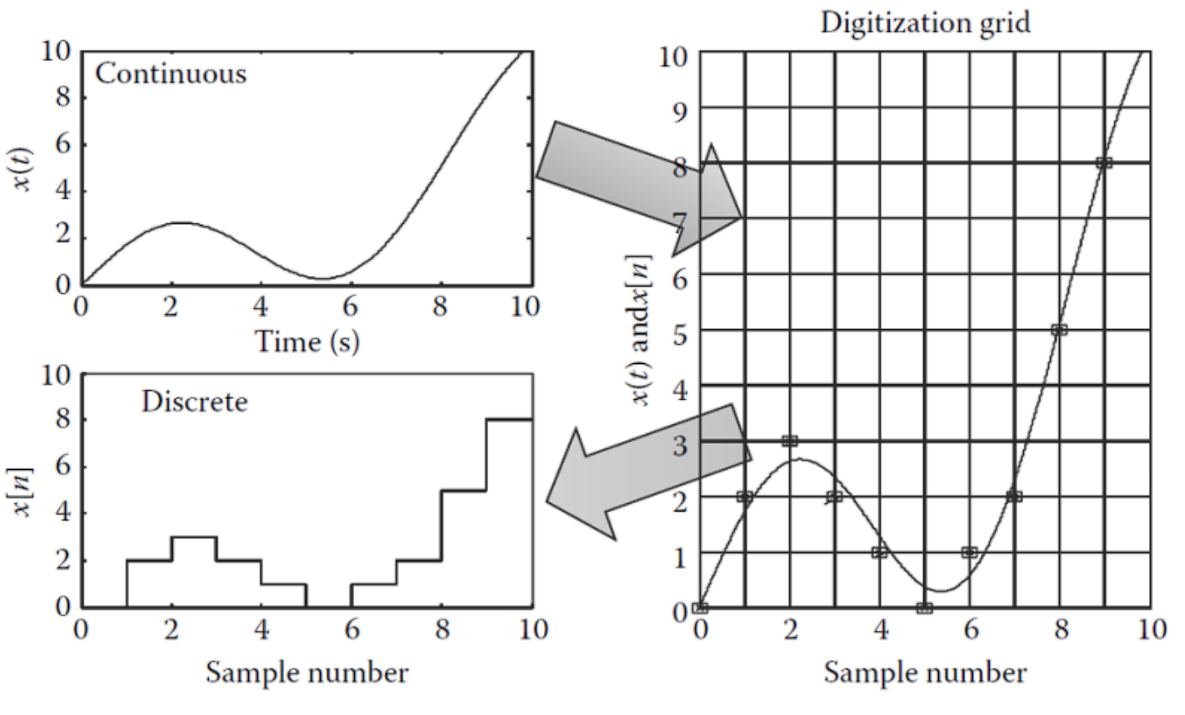
\includegraphics[width=0.6\textwidth]{images/discretization.png}
\end{figure} 
We have to consider a limited (and finite) number of possible amplitudes for the signal, due to the fact that these information are stored in a computer as bytes of data.  This is a two-step process, first we discretize time, by considering only the function samples on some equi-distant time steps, and then we discretize the amplitude by considering the nearest value that can be represented in bit.\begin{itemize}
     \item \textbf{Sampling}: time discretization.
     \item \textbf{Quantization}: amplitude discretization.
\end{itemize}
When we quantize a signal $x(t)$ we allow only a finite number of available levels for the amplitude, let's denote $x^*(t)$ the quantized signal (still continuous in time).
By doing that, we are introducing an error between the real signal and the quantized one, this profile is called \textit{quantization noise} and is exactly the difference between the quantized signal and the original one\begin{equation}
     n(t)=x(t)-x^*(t).
\end{equation} 
We call \textit{allowed levels} the values of discrete amplitudes that we consider in $x^*(t)$.\begin{itemize}
     \item allowed levels: $X=\{a_1,a_2\dots a_k\}$
     \item original signal: $x(t)$
     \item let $t_0$ to be a particular time value:\begin{equation}
          x^*(t_0)=\arg\min_{a\in X}\|x(t)-a\|.
     \end{equation}
\end{itemize}
\begin{figure}[H] 
     \centering
     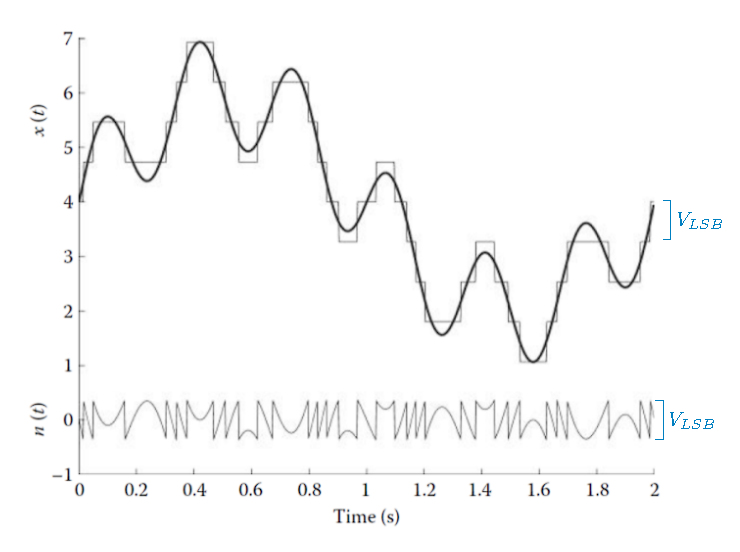
\includegraphics[width=0.5\textwidth]{images/quantization.eps}
\end{figure}
The range of the error is exactly the distance between two allowed levels. In the noise $n(t)$, every value of the image is equally probable to be found (there is a uniform probability distribution). To reduce the noise, we have to choose a smaller distance between two allowed levels.

Let $V_{LSB}$ to be the distance between two close amplitude levels. The noise $n(t)$ is uniformly distributed between $[-\nicefrac{V_{LSB}}{2},\nicefrac{V_{LSB}}{2}]$. So the expected value of the noise is 0 and the standard deviation is $$\sigma=\frac{1}{\sqrt{12}}V_{LSB}\simeq 0.29V_{LSB}.$$
The quantization is made in binary and is characterized by the number of bits involved. If \texttt{bits} is the number of bits, the number of allowed levels is $2^{\texttt{bits}}$. The range of the measured signal is\begin{equation}
     range=V_{LSB}\cdot 2^{\texttt{bits}}
\end{equation}
for example, if we are measuring a signal that we know can change between 0 and 14 mV, and we are storing each  sample with 8 bit, the distance between two allowed levels is\begin{equation}
      14=V_{LSB}\cdot 2^{8}\implies V_{LSB}=0.0546875 \text{ mV}.
\end{equation}
The original signal measured already contain some noise due to artifacts or other sources. The total noise of the quantized signal is given by the original signal noise and the noise provided by the quantization\begin{equation}
     noise_{tot}=\sqrt{(noise_{signal})^2+(noise_{quant})^2}
\end{equation}
is important to use a sufficient number of bits in order to decrease the quantization noise such that is negligible (or at least comparable) respect to $noise_{signal}$.\bigskip 

Other than the quantization, is important to perform a good \textit{sampling} of the signal. A signal is \textbf{properly sampled} if we are able to reconstruct the analog signal from the sampled signal with no error.
The Nyquist-Shannon theorem states that 
a time continuous signal can be properly sampled only if does not contain frequency components above one half of the sampling rate.\bigskip

When sampling a signal, the values of this in the points not covered by the sampling interval are necessarily lost, it is clear that a smaller sampling time $T_C$ equates to greater precision. We also want to reconstruct the signal from digital to analog so that it is as faithful as possible to the desired signal.\bigskip

For a time-continuous signal $x(t)$, we denote $X(j\omega)$ it's spectrum given by the Fourier transform. Consider the spectrum of a (continuous) band-limited signal $X(j\omega)$
\begin{center}
    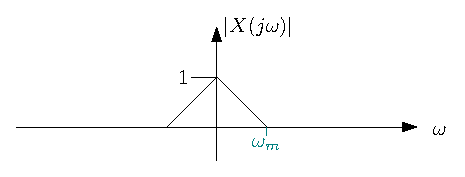
\includegraphics[width=0.7\textwidth]{images/segLimitatoBanda.eps}
\end{center}
When this is sampled, the magnitude of the sampled frequency response $|X^*(j\omega)|$ will be scaled by a factor $\frac{1}{T_C}$. Furthermore, sampling a continuous signal over time is equivalent, in the frequency domain, to multiplying the original spectrum of the signal by a train of pulses. This multiplication has the effect of periodically replicating the original spectrum, thus creating \textit{complementary components}.
\begin{center}
    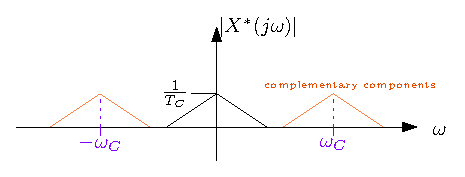
\includegraphics[width=0.7\textwidth]{images/segLimitatoBanda2.eps}
\end{center}
We denoted $\omega_C=\frac{1}{T_C}$ the sampling rate.
The original signal $|X(j\omega)|$ can be reconstructed with a reconstruction filter $G_R$ defined as follows
$$ G_R(j\omega)=\begin{cases}
    T_C \text{ if }|\omega|\le \frac{\omega_C}{2}\\ 
    0 \text{ else}
\end{cases}$$
it is clear that $|X(j\omega)|=|G_R(j\omega)|\cdot |X^*(j\omega)|$
\begin{center}
    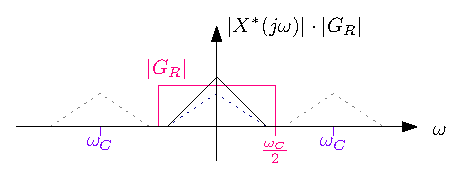
\includegraphics[width=0.7\textwidth]{images/segLimitatoBanda3.eps}
\end{center}
This example makes the following result clear.
\begin{boxtheorem}{Nyquist, Shannon}{}
     Given the signal $X(j\omega)$, let $\omega_m=\max\{\omega_i\ | \ X(j\omega_i)>0\}$ be the maximum frequency allowed by the signal. In order to reconstruct the signal without errors from a sampled version $X^*(j\omega)$, it is necessary that the sampling frequency $\omega_C$ is at least twice $\omega_m$: \begin{equation}
          \omega_C\ge 2\omega_m.
     \end{equation}
\end{boxtheorem}
If this were not the case, the complementary bands would overlap with the original band, this phenomenon is called \textbf{aliasing}, and involves a \textit{corrupt} signal construction, regardless of the filter used. For the signal considered in the previous example, a sampling frequency $\omega_C$ is considered less than $2\omega_m$
\begin{center}
    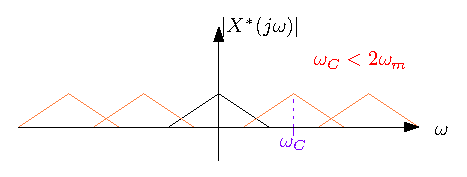
\includegraphics[width=0.7\textwidth]{images/segLimitatoBanda4.eps}
\end{center}
The filter is applied
\begin{center}
    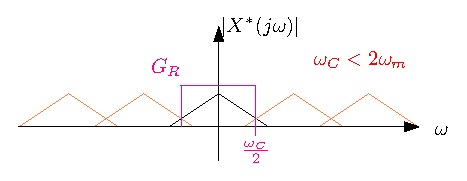
\includegraphics[width=0.7\textwidth]{images/segLimitatoBanda5.eps}
\end{center}
the reconstructed signal is corrupted
\begin{center}
    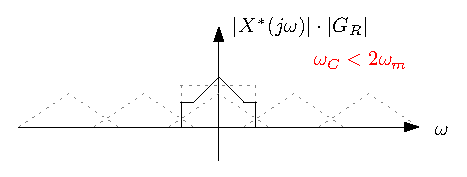
\includegraphics[width=0.7\textwidth]{images/segLimitatoBanda6.eps}
\end{center}
Real signals have components at sufficiently high frequencies that a sufficiently high sampling frequency is not possible, therefore it is inevitable that there is aliasing, which is why analog filters are used upstream before sampling.
\subsection{Randomness in Signals}
In real life, we deal with systems that are not completely deterministic, and they have some intrinsic randomness. We need some tools to evaluate the properties of systems of this kind.

The word ''random'' can refers to different levels of complexity in the context of stochastic behaviors. A whole signal can be ''random'', and can't be known in advance, but we can predict the probability that the signals (for example) reaches at some point a given value.\bigskip 

A random process in our context, assign a probability to every possible EEG signals over time that we might observe, when we measure the EEG we have a \textbf{realization} of the random process.\bigskip 

In the context of statistic, the true mean of a given random variable $X$ can be approximated by considering $N$ observation $\{x_i\}:\subset Im(X)$\begin{equation}
     \bar X=\frac{1}{N}\sum_{i=0}^{N-1}x_i
\end{equation}
$Im(X)$ is the image set of the variable $X$.
We denote $\mu_X$ the real mean:\begin{equation}
     \lim_{N\rightarrow \infty}\bar X=\mu_X
\end{equation}
this estimation is called \textbf{sampled mean}. The real mean is a deterministic value (not stochastic) but it is unknown. The mean is a measure of \textit{central tendency}, so, where around each value the observation aggregates. The \textbf{variance} $\sigma_X^2$ instead, is a measure of how much the data points in a set differs from the mean, calculated as the average of the squared deviations. Can be estimated through the observation of $N$ samples $\{x_i\}$, resulting in the \textbf{sampled variance}:\begin{equation}
     s_X^2=\frac{1}{N-1}\sum_{i=0}^{N-1}(x_i-\bar X)^2
\end{equation}
of course is true that\begin{equation}
      \lim_{N\rightarrow \infty} s_X^2=\sigma_X^2.
\end{equation} 
The \textbf{standard deviation} is just the square root of the variance:\begin{equation}
     s_X=\sqrt{\frac{1}{N-1}\sum_{i=0}^{N-1}(x_i-\bar X)^2}.
\end{equation}
The currents produced by the population of neurons are not deterministic, hence it is a stochastic process, on which each EEG measurement over time is a realization. To get the sample mean of an EEG under static conditions (the patient remain still) we can register $N$ trials, and then average all the trials to get an idea of the mean value for the EEG, as shown in figure \ref{AVG_EEG}.
\bigskip

An important tool used in stochastic signal theory is the \textit{Gaussian White Noise}, the amplitude of that signal at any given time follows a normal distribution with zero mean. This means small fluctuations are common, while extreme spikes are rare.
\begin{center}
    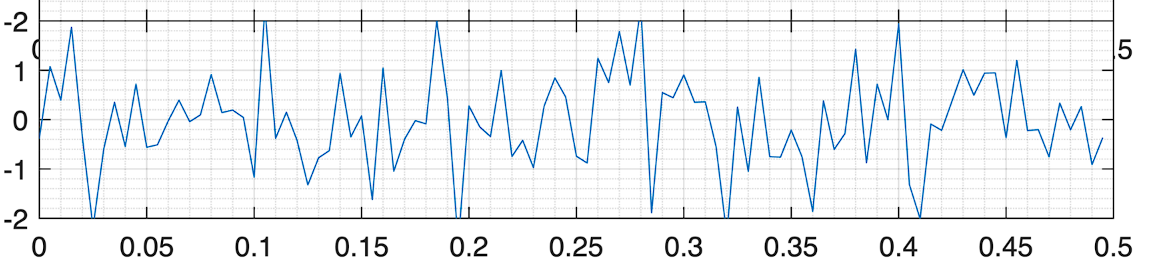
\includegraphics[width=0.7\textwidth]{images/gwn.png}
\end{center}
If we sample a Gaussian white noise and we plot the histogram, where on the $x$ axis we have the observed amplitudes and on the $y$ axis the number of occurrences for each observed value, we will  have a bell curve (normal distribution) with the sampled mean near to zero.
\begin{figure}[H] 
     \centering
     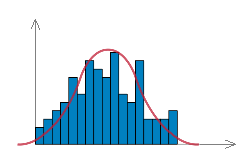
\includegraphics[width=0.4\textwidth]{images/hisogram_gwn.eps}
     \caption{Example of histogram of the Gaussian white noise.}
\end{figure}
Why is called ''white''? The term is an analogy to white light. Just as white light contains all frequencies of the visible spectrum with the same intensity, white noise contains all sound (or signal) frequencies with the same power. In technical terms, it is said to have a constant power spectral density.\begin{itemize}
     \item Each value (sample) extracted from the signal is totally independent from the previous and subsequent ones.
     \item  Knowing the value of the signal at time $t$ gives you absolutely no information about what the value will be at time $t+1$.
\end{itemize}
\begin{boxtheorem}{Central Limit}{}
     Let $\{X_1,X_2\dots X_N\}$ to be a countable set of $N$ identically distributed random variables, and let $Z$ to be the average variable:\begin{equation}
          Z=\frac{1}{N}\sum_{i=1}^NX_i.
     \end{equation}
     With the number of random variables growing to infinity: $N\rightarrow\infty$, $Z$ tends toward a normal distribution, even if the original variables $\{X_1,X_2\dots X_N\}$ are not normally distributed:\begin{equation}
          \lim_{N\rightarrow \infty}\frac{1}{N}\sum_{i=1}^NX_i=\mathcal N.
     \end{equation}
\end{boxtheorem}
The mean of this resulting ''almost'' normal distribution will be the mean of $X_i$, all the variables have the same distribution, so we just write $X$\begin{equation}
     \mu_Z=\mu_X
\end{equation}
the variance and the standard distribution are\begin{align}
     &\sigma_Z^2=\frac{1}{N}\sigma_X^2\\ 
     &\sigma_Z=\frac{1}{\sqrt N}\sigma_X.
\end{align}
\section{Spectral Analysis}
There are four kinds of ways to perform the Fourier analysis on a function:\begin{itemize}
     \item Let $x(t)$  be a continuous function periodic in $[0,T]$. We know that this function is a linear combination of an infinite (but countable) number of trigonometric functions.
     The coefficients of it's Fourier series are given by the complex-valued function $X:\Z\rightarrow\C$  defined as follows: \begin{align}
          &X[m]=\frac{1}{T}\int_{0}^{T}x(t)\exp(-j2\pi mft)dt, \ \ \ m\in \Z\\ 
          &f=\nicefrac{1}{T}
     \end{align}
     We are denoting $j=\sqrt{-1}$ the imaginary unit.
     \item An \textit{aperiodic} continuous function $x(t)$ is a linear combination of an infinite (not countable) number of basic harmonics, it's fourier transform identifies the coefficients of this linear combination:\begin{equation}
          X(f)=\int_{-\infty}^{+\infty}x(t)\exp(-j2\pi ft)dt.
     \end{equation}
     \item A discrete periodic function $x[n]$ of $N$ samples can be analyzed in the frequency domain through it's discrete time Fourier series, which it's coefficients are given by\begin{align}
          &X[m]=\sum_{n=1}^N x[n]\exp(-j2\pi m n \nicefrac{1}{N})\\ 
          &m=0,\pm 1, \pm 2,\dots \pm \nicefrac{N}{2}.
     \end{align}
     \item For an aperiodic discrete function $x[n]$ it's discrete time Fourier transform is given by\begin{equation}
          X(f)=\sum_{n=-\infty}^{+\infty}x[n]\exp(-j2\pi nf ).
     \end{equation}
\end{itemize}
We are interested in decomposing signals into sum of sinewaves, in order to analyze a signal in the frequency domain. In our context, we deal with time limited and discrete signals that are sampled, like the EEG,  given in their time domain, and we will apply the discrete Fourier transform (DFT) to get their bandwidth limited and sampled representation in the frequency domain. Later we will see how a time limited signal is equivalent to a periodic signal, so formally, the DFT applies to periodic signals.
\begin{boxdefinition}{}{}
     A signal $x$ is said to be \textit{bandwidth limited} if there exists a maximum frequency $M$ such that $X[M]=0, \ \forall |m|>M$.
\end{boxdefinition}
\noindent Notice how we usually denote $x$ a signal in the time domain and $X$ it's frequency representation. 
Let's consider a sinewave characterized by three parameters, the amplitude $A$, the frequency $f$ and the phase $\phi$\begin{equation}\label{sinewave}
     A\cos(2\pi ft+\phi)
\end{equation}
we know that each complex number $z\in \C$ can be represented in exponential form as follows:\begin{equation}
     z=Ae^{j\phi}
\end{equation}
and the amplitude and phase can be extracted as follows \begin{align}
     &A=|z|\\ 
     &\phi = \angle z
\end{align}
the continuous wave in equation \eqref{sinewave} can be identified by a complex number (that represent the amplitude and the phase) and a real number $f$ that is the frequency. If the frequency is fixed, the wave is identified exactly by a single complex number $ z=Ae^{j\phi}$.

Each discrete time sampled signal is a periodic signal made up by the sum of a finite number of sinewaves of different frequencies, represented as complex numbers, we are interested in the map between the signal $x[n]$ and the set of complex numbers $X[m]$ that identifies these sinewaves.
\begin{figure}[H] 
     \centering
     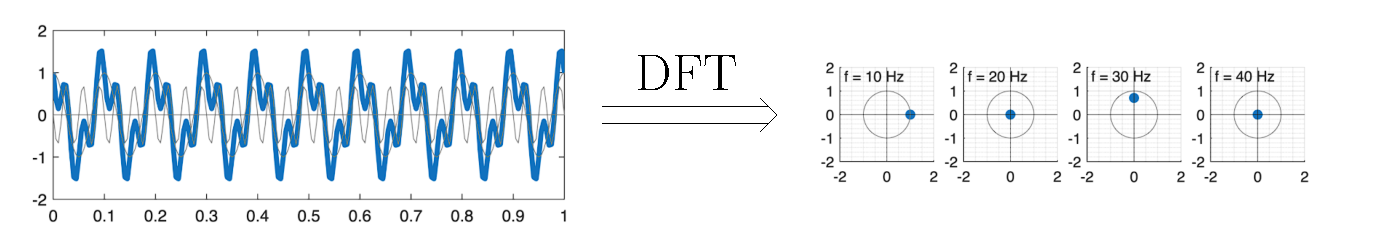
\includegraphics[width=\textwidth]{images/DFT.eps}
\end{figure}
The DFT is exactly the relationship between the time domain samples $x[n]$ of the signal and the amplitude and phase relative to a specific frequency $m$:\begin{equation}\label{DFT}
     X[m]=\sum_{n=0}^{N-1}x[n]\exp(-j2\pi mn\nicefrac{1}{N})
\end{equation}
the product over the summation $\sum_{n=0}^{N-1}x[n]\exp(-j2\pi mn\frac{1}{N})$ is a  \textbf{similarity measure} between the signal $x[n]$ and the specific harmonic $\exp(-j2\pi mn\frac{1}{N})$ of frequency $m$.\begin{quote}
     \textit{the contribution of the sinewave in the signal is given by the dot product between these two.}
\end{quote}
In fact, in the vector space of continuous function periodic in $[0,T]$, the dot product between two functions $f$ and $g$ is given by\begin{equation}
     \langle f,g\rangle=\frac{1}{T}\int_0^T f(t)\overline{g(t)}dt
\end{equation}
where $\overline{g(t)}$ is the complex conjugate of $g(t)$. In the DFT, we add the minus in the exponential to take the complex conjugate of the sinewave. 

From a series of complex numbers $X[m]$ that represent the signal in the frequency domain, we can reconstruct each sample of the time domain representation through the anti transformation:\begin{equation}
     x[n]=\frac{1}{N}\sum_{m=0}^{N-1}X[m]\exp(j2\pi mn\nicefrac{1}{N}).
\end{equation}
The transformation in equation \eqref{DFT} is linear in the samples $x[n]$. Let $\mathbf x$ to be the vector of time samples\begin{equation}
     \mathbf x=\begin{pmatrix}
          x[0]&x[1]\dots x[N-1]
     \end{pmatrix}^T
\end{equation}
and $\mathbf X$ to be the vector of the frequency representation\begin{equation}
     \mathbf X=\begin{pmatrix}
          X[0]&X[1]\dots X[N-1]
     \end{pmatrix}^T
\end{equation}
The DFT is a linear transformation $W$:\begin{equation}
     \mathbf X = W\mathbf x
\end{equation}
where $W$ is the $N\times N$ matrix defined as follows\begin{equation}
     W_{n,m}=\exp\left(-j\frac{2\pi}{N}mn\right).
\end{equation}
Let's recap some relationship between the sampling quantities for periodic signals:
For a time domain signal sampled with the first sample in time zero and the last sample in time $T$ (the signal is $T$-periodic), the frequency domain will be $\Delta f$ discrete where\begin{equation}
     \Delta f=\frac{1}{T}
\end{equation}
i.e., each sample in the frequency domain is at distance $\Delta f$, furthermore, the sampling time is $T_S$ (distance between each sample in the time domain) and\begin{equation}
      \Delta f=\frac{1}{T}=\frac{1}{NT_S}
\end{equation}
where $N$ is the number of samples. The frequency domain is $f_S$-periodic, where \begin{equation}
     f_S=\frac{1}{T_S}.
\end{equation}
\begin{figure}[H] 
     \centering
     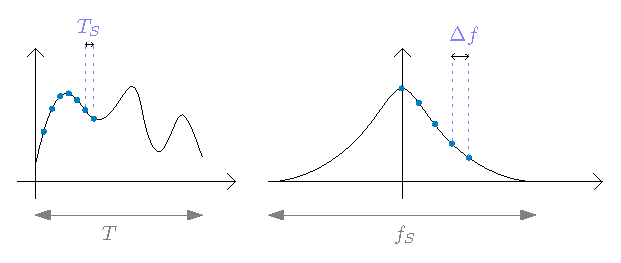
\includegraphics[width=0.7\textwidth]{images/sampling_values.eps}
\end{figure}
If we take the Fourier transform of a sampled signal, we will have a periodic frequency domain representation, in a dual way, by taking the anti-transformation of a sampled frequency spectrum, we will have a periodic signal.

\begin{table}[H]
    \centering
    \caption{Sampling relations for periodic signals}
    \label{tab:campionamento}
    \begin{tabular}{cll}
        \toprule
        \textbf{Notation} & \textbf{Description} & \textbf{Relation} \\
        \midrule
        $T$ & Total Duration / Signal Period & $T = N \cdot T_S$ \\
        $T_S$ & Sampling period (time between samples) & $T_S = 1 / f_S$ \\
        $N$ & Total number of samples & $N = T / T_S$ \\
        $\Delta f$ & Frequency resolution (distance between samples in freq.) & $\Delta f = \frac{1}{T} = \frac{1}{N \cdot T_S}$ \\
        $f_S$ & Sampling rate & $f_S = \frac{1}{T_S}$ \\
        \bottomrule
    \end{tabular}
\end{table}

To represent graphically the DFT of a signal we use two plots, one for the magnitudes of each sample, one for the phases:
\begin{figure}[H] 
     \centering
     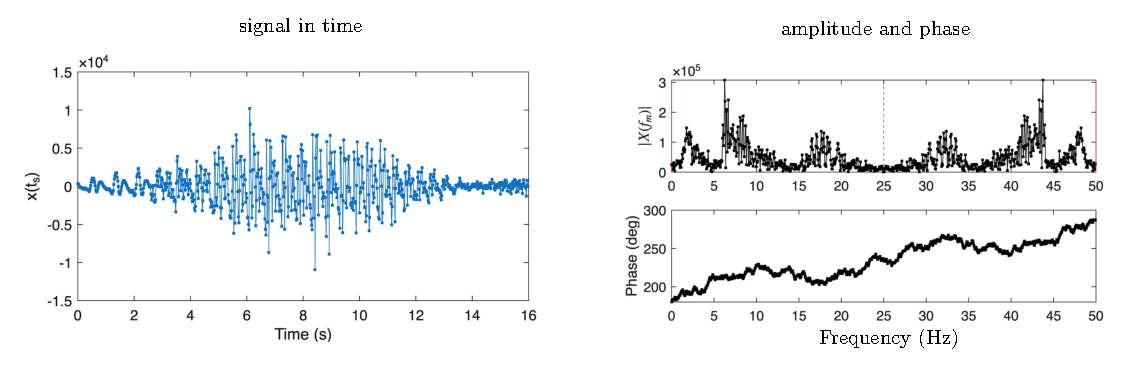
\includegraphics[width=0.9\textwidth]{images/graphical_repre.eps}
\end{figure}
The magnitude spectrum is symmetrical, while the phase spectrum is anti symmetrical, since a real sample satisfies the following relation:\begin{equation}
     x(t)\in\R \xLeftrightarrow{\mathcal F} X(f)=X^*(-f)
\end{equation}
where $X^*$ is the complex conjugate of $X$. The left side $f<0$ does not contain any information, so it is practical to represent the plots only for positive frequencies $f\ge 0$.\bigskip 

\noindent\textbf{Example}: Let's consider two signals, one have the power spread to all the spectrum (white noise), while the other have most of it's power concentrated in a limited frequency band (sine wave). Assume that we have a signal that is a sine wave corrupted by this white noise, and we would like to see the sine wave within noise.
\begin{figure}[H] 
     \centering
     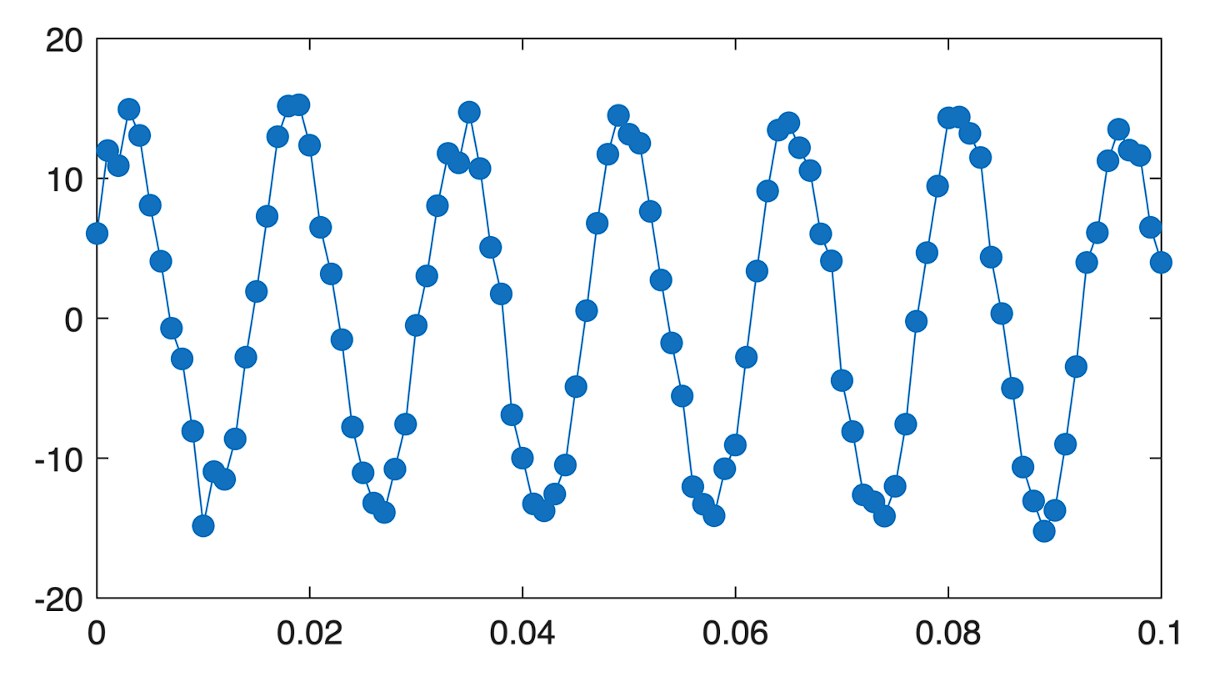
\includegraphics[width=0.5\textwidth]{images/corrupted_sin.png}
\end{figure}
The spectrum of this signal is\begin{figure}[H] 
     \centering
     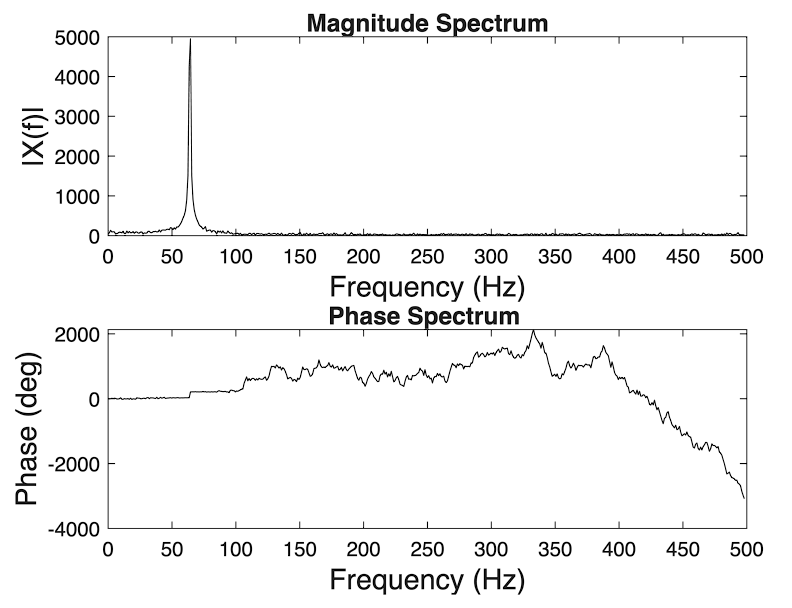
\includegraphics[width=0.4\textwidth]{images/corrupted_sin2.png}
\end{figure}
The magnitude spectrum is not a perfect Dirac delta, we can see the ''leakage'' due to the white noise, even if in the time domain the signal is pretty corrupted, in the frequency domain the peak is still visible.\subsection{Zero Padding}
\noindent Now we show a technique for spectral estimation, called \textit{Zero Padding}:
Let's consider a signal $x(t)$, that last half a second, and is a triangular wave (rising ramp then falling ramp). We sample the signal with a sampling frequency of 1 kHz ($T_S=0.001$ s).
\begin{figure}[H] 
     \centering
     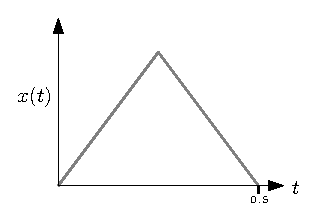
\includegraphics[width=0.3\textwidth]{images/triangle.eps}
\end{figure}
So we take 500 samples of the signal. We can observe the spectrum of frequencies from 0 to 500 Hz. The distance between each sample in the spectrum is $\Delta f=\frac{1}{T}=2$ Hz. Let's take into account only the first 6 samples of the spectrum (from $f=0$ Hz to $f=10$ Hz):
\begin{figure}[H] 
     \centering
     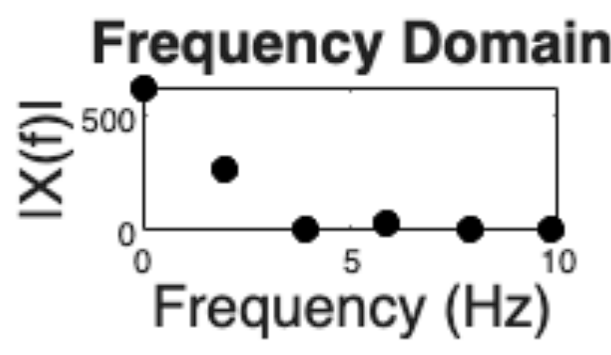
\includegraphics[width=0.4\textwidth]{images/first6Samples.png}
\end{figure}
Now, let's take the same original signal $x(t)$,  we extend this signal by adding (after the first half second) a zero value for 1.5 seconds:
\begin{figure}[H] 
     \centering
     \includegraphics[width=0.7\textwidth]{images/triangle2.eps}
\end{figure}
We are not adding any information, now that $T=2$, the distance between two points in the spectrum will be $\Delta f=\frac{1}{2}$ Hz, i will have a more dense sampling in the spectrum:
\begin{figure}[H] 
     \centering
     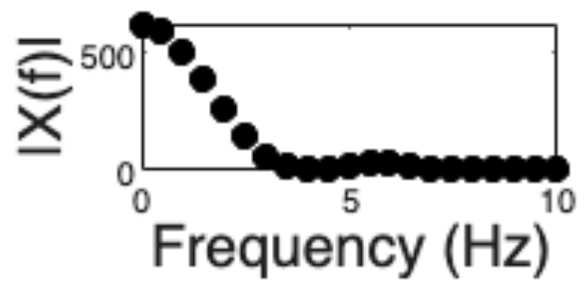
\includegraphics[width=0.4\textwidth]{images/first6Samples2.png}
\end{figure}
\begin{boxdefinition}{Zero Padding}{}
     Adding a row of zeros at the end of the signal allows to (artificially) increase the spectral
     resolution, even with dealing with short signals.
\end{boxdefinition}
This does not add any information to the spectrum, it is used just to make the spectrum more ''visible'' and better understandable: it is \underline{just a visual improvement}.
\subsection{Windowing}
When we want to estimate  the properties of a stochastic signal, we need (in principle) to know the signal for an infinite amount of time. Let's see what happens (even to a deterministic signal) when this is not possible.\bigskip 

Let $x(t)$ to be a signal defined on all the real line $\R$, we don't have access to all the signal, but only to a short recording $x'(t)$:
\begin{figure}[H] 
     \centering
     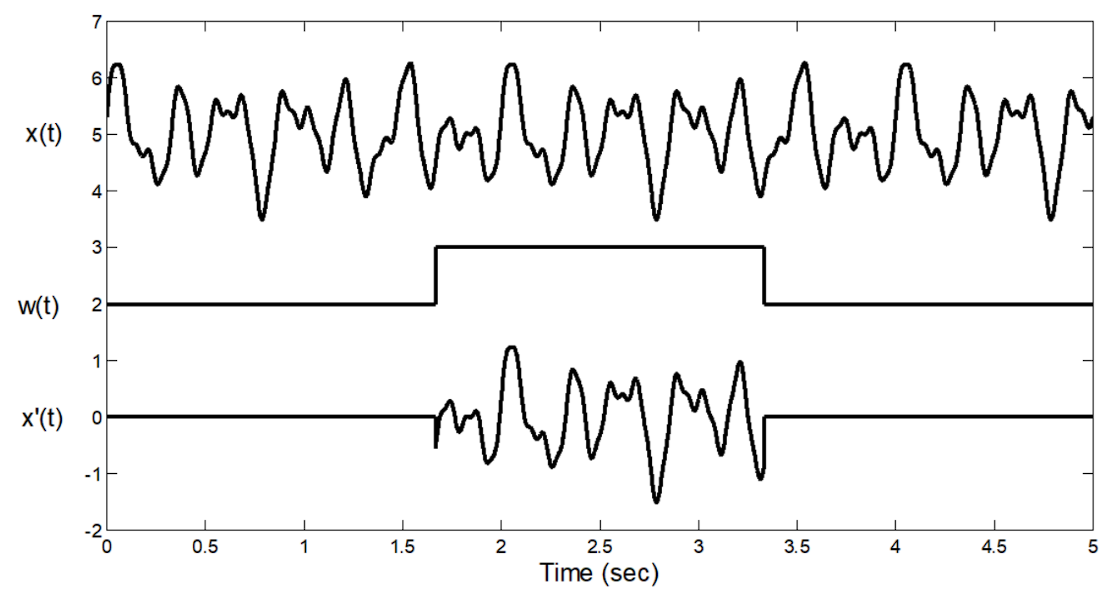
\includegraphics[width=0.6\textwidth]{images/recording.png}
\end{figure}
\textit{Question}: How does the spectral properties of $x'(t)$ relates to the spectral properties of the original infinite time signal $x(t)$?

We have introduced the \textbf{window function} $w(t)$, that is zero before and after the recording time, and 1 during the period of recording. $x'(t)$ is just the result of $x(t)w(t)$. What happens in the frequency domain? We know that multiplication in the time domain is equivalent to convolution in the frequency domain:\begin{equation}
     x'(t)=x(t)w(t) \xLeftrightarrow{\mathcal F} X(f)*W(f)=X'(f)
\end{equation}
The only thing that we can compute is the Fourier transform of $x'(t)$, denoted $X'(f)$, the spectrum of the rect function $w(t)$ is the sinc function: $W(f)=\frac{\sin f}{f}$.\bigskip 

When we convolute the original spectrum with the sinc wave we have a spectrum leakage, the power of each sine component of $x(t)$ is ''spread'', and no anymore concentrated. \bigskip 

Since every $x(t)$ can be decomposed as an infinite sum of sinewaves, we can see this phenomena by looking at how the convolution with $W(f)$ acts when $x(t)=\sin(2\pi f_0 t)$, in this case $X(f)$ results in two concentrated impulse (Dirac delta) in $f=f_0$ and $f=-f_0$
\begin{equation}
     X(f)=\frac{1}{2i} [\delta(f - f_0) - \delta(f + f_0)]
\end{equation}
convolving this impulse centered at $f_0$ with $\frac{\sin f}{f}$ results in the identical sinc wave centered on $f_0$. The finite amount of time of recording produce \textbf{spectral leakage}.\bigskip

The multiplication with the window function $w(t)$ introduce discontinuity, this is another point of view to see the cause of leakage, this discontinuity makes the signal $x'(t)$ ''fast'', with very high frequencies, so it's creating energy at high frequencies that was not there.\begin{boxobservation}{}{}
     Discontinuity introduce energy at new frequencies.
\end{boxobservation}
Instead of starting and stopping the recording, that are modeled by the rect function that is sharp, we might start a recording with a zero gain, rise the gain slowly, and then at the end, reduce the gain, having smooth transition, defining a new windowing function.
\begin{figure}[H] 
     \centering
     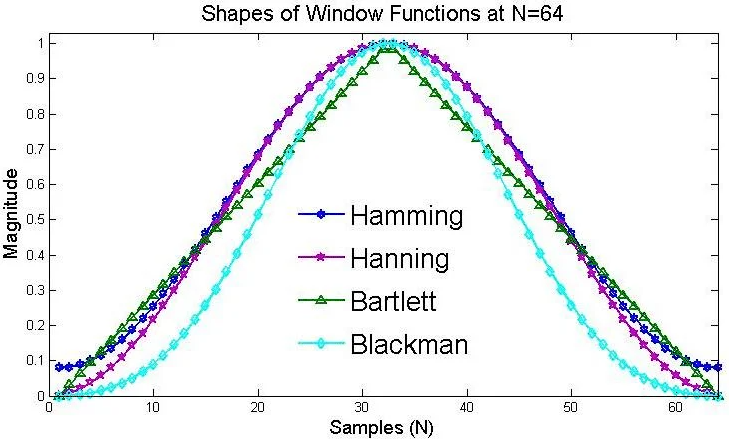
\includegraphics[width=0.5\textwidth]{images/windowingFunctions.png}
     \caption{Some examples of non rectangular windowing functions.}
\end{figure}
Let's take in account the Hamming and Blackman windowing functions, these two introduce less leakage respect to the rect function.
\begin{figure}[H] 
     \centering
     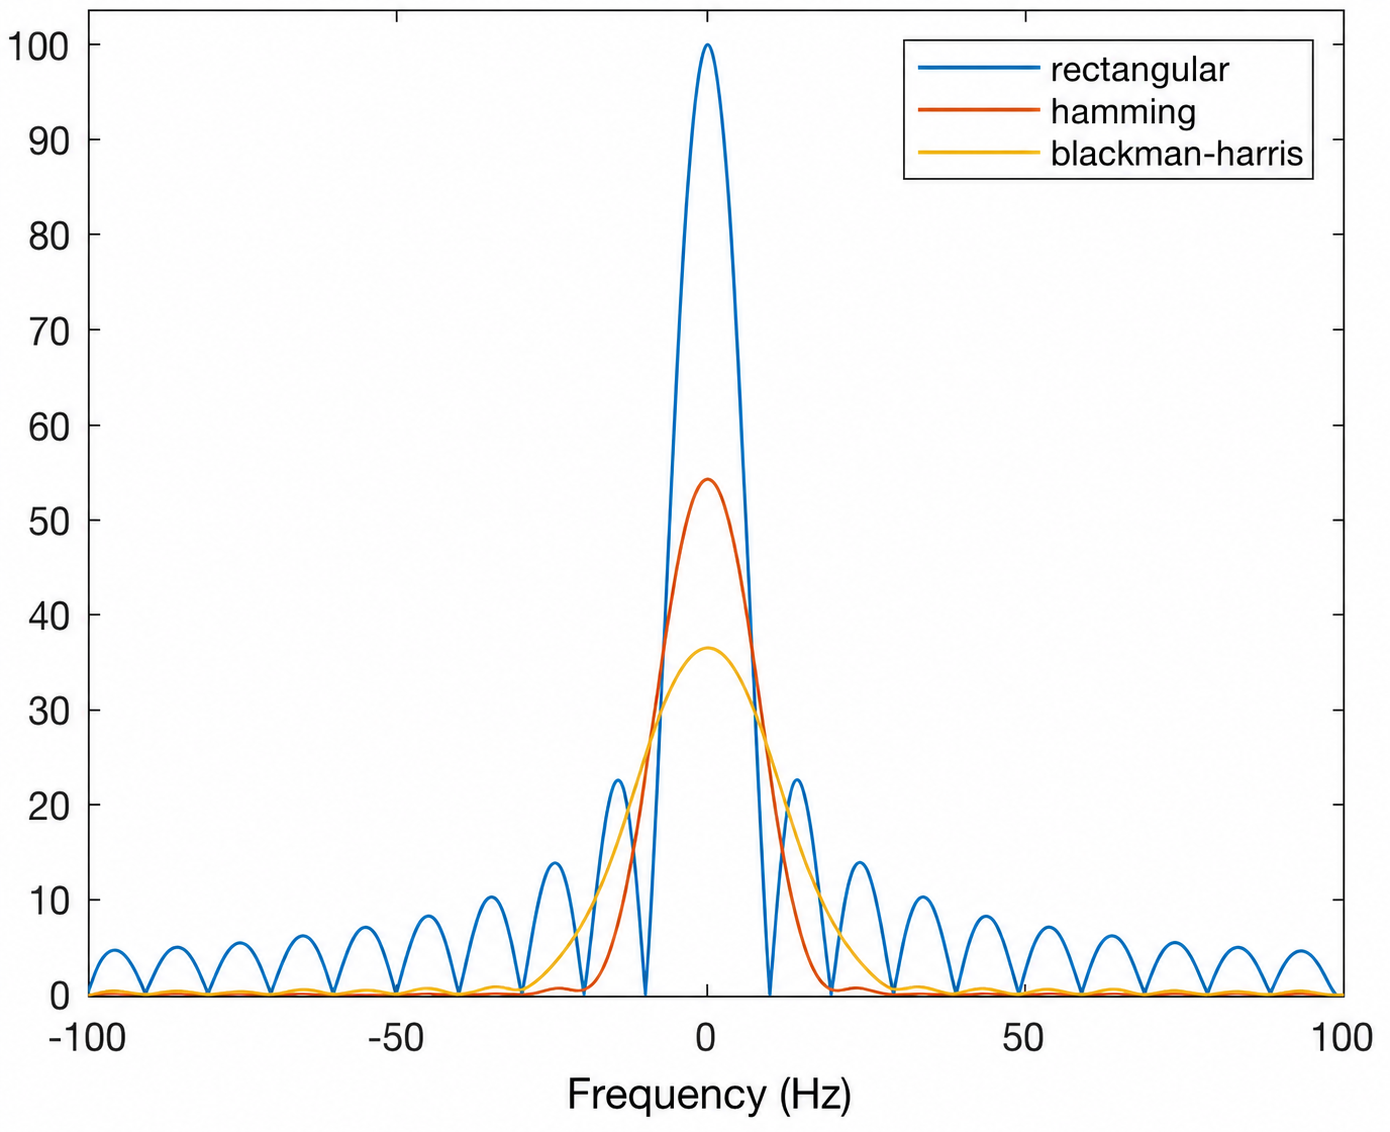
\includegraphics[width=0.45\textwidth]{images/windowingFunctionsFT.png}
     \caption{Fourier transforms of the windowing functions.}
\end{figure}
For the Fourier transforms of the windowing functions we define the \textbf{main lobe} and the \textbf{secondary lobes}:\begin{itemize}
     \item The main lobe is the central peak, the widest and with the greatest amplitude. The width of the main lobe defines how close two frequency components can be for the system to distinguish them as two separate peaks. The narrower the main lobe, the better the resolution. However, it is physically impossible to have an infinitely narrow main lobe (the ideal would be a Dirac pulse), so a compromise is accepted.
     \item The secondary lobes are the minor oscillations that propagate to the sides of the main lobe. They determine the spectral leakage (or dispersion). When a signal has a strong component at a certain frequency, the energy of this component ''leaks'' through the secondary lobes into other nearby frequencies. This creates artifacts and reduces the dynamic range of the system. The lower the amplitude of the secondary lobes compared to the main lobe, the lower the background noise caused by leakage.
\end{itemize}
It is not possible to simultaneously minimize the width of the main lobe (better resolution) and the width of the secondary lobes (less leakage), there is an intrinsic trade-off between these two elements.
With a logarithmic scale for the Fourier transforms we can see the difference in the primary and secondary lobes.
\begin{figure}[H] 
     \centering
     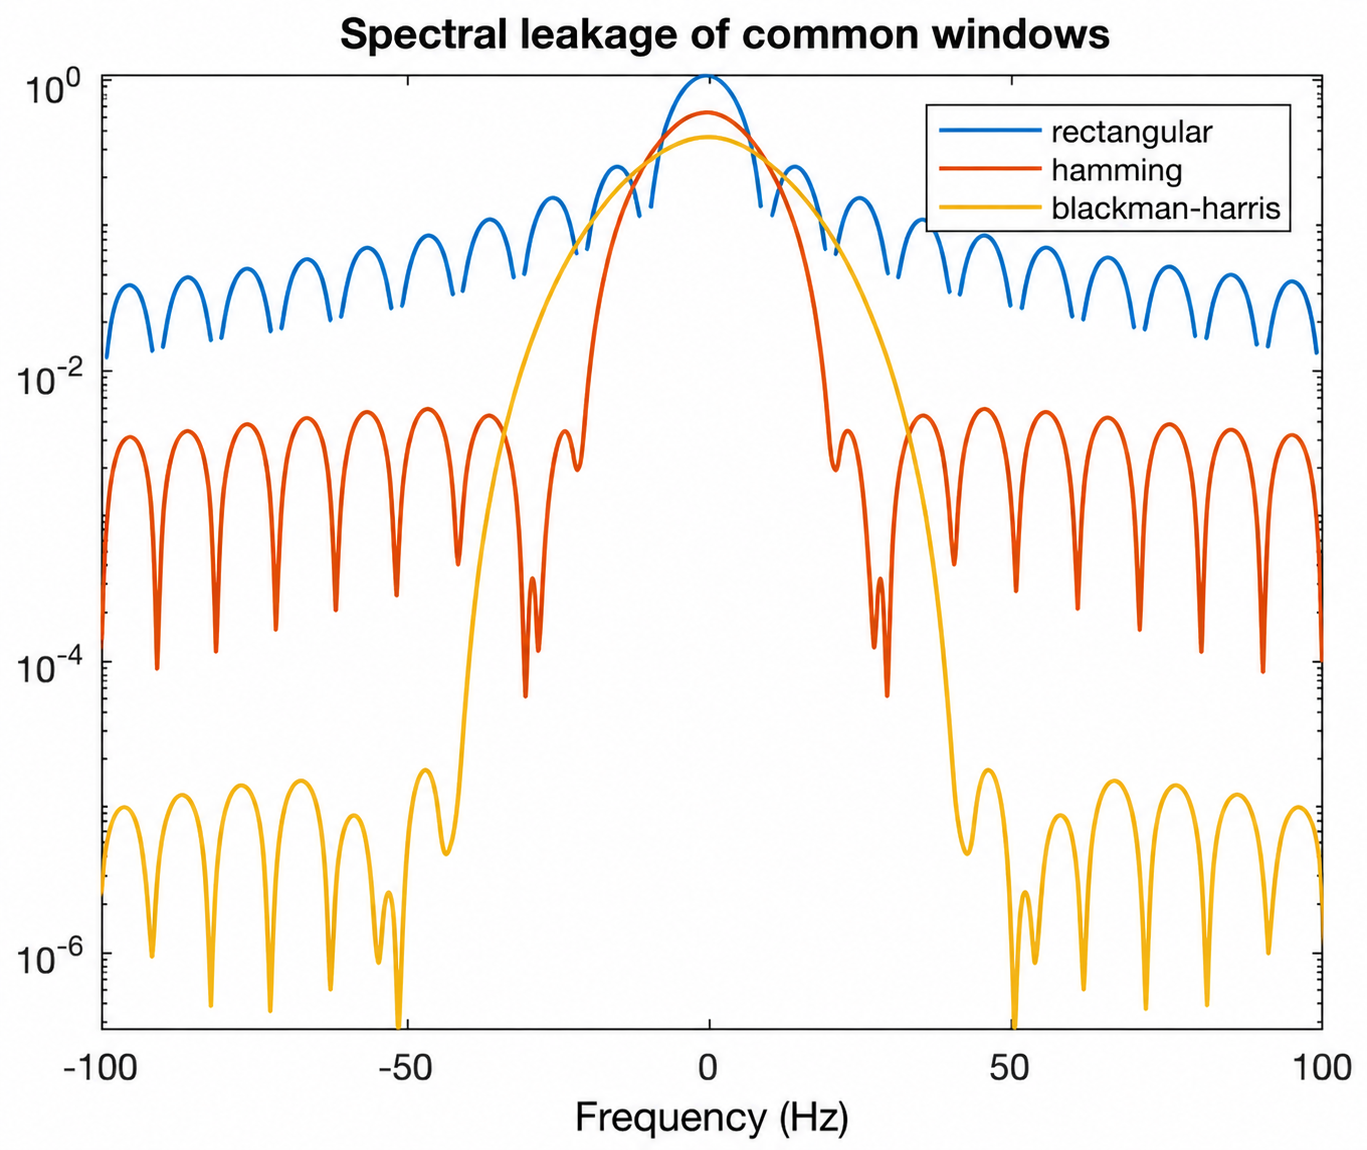
\includegraphics[width=0.45\textwidth]{images/windowingFunctionsFT2.png}
     \caption{Fourier transforms of the windowing functions.}
\end{figure}
\subsection{Stochastic Signals}
\begin{boxdefinition}{Power Spectrum (Density)}{}
     The power spectrum describes the power of the signal in each frequency band of the spectrum. A basic
estimation called \textbf{periodogram}  can be obtained by taking the square of the absolute value of the DFT of the
signal.\begin{equation}
     PS(f)=|DFT(x(t))|^2.
\end{equation}
\end{boxdefinition}
This is not the formal definition, but is the one required for our purposes. The sum of the amplitudes of the DFT is the total energy of the signal, the power spectral density (PSD) is the Power Spectrum divided by the width of frequency bins.

Note that the periodogram is not appropriate to analyze a stochastic signal. In fact, estimating the properties
of the generating stochastic process from a single realization of the signal yields a large variance of the
estimate (though it is unbiased it is a non consistent estimator).\bigskip

A stochastic process is the source that generates a signals with some statistical properties, a realization is one specific instance generated from that process, an EEG is a realization of the brain that is the stochastic process that generates the time varying potential on the scalp. To estimate the properties of the stochastic process, we need several realizations of it.

A stochastic process is \textbf{ergodic} if a single realization is enough to describe it completely: Everything that the process can express is always summarized in just one realization. Despite that, we would need that realization to be defined in $t\in\R$ (whole time history of the signal), practically this is never the case, since we always register a time limited window of a signal.

The best thing that we can do is understand what happens when we register this time limited realization.\bigskip 

The periodogram is not a great estimator for the spectral properties of the signal, is unbiased but it is not consistent: even if we take a longer signal, the variability of the spectrum will not reduce.
How can we get a better estimator? Instead of having one estimate, we take the average of several estimate: 
\begin{itemize}
     \item We record an EEG for one second.
     \item We have 1000 samples.
     \item We take a windowing function and compute the periodogram.
     \item the resolution $\Delta f=\frac{1}{T}=1$ Hz depends only on the length of the signal.
     \item Assume we are not interest in the 1 Hz resolution, assume we can  accept 2 Hz resolution. So we need just $\frac{1}{2}$ seconds of signal.
     \item We take the first  $\frac{1}{2}$ seconds of signal and compute the periodogram, and do the same for the remaining  $\frac{1}{2}$ seconds.
     \item We have two instances of the periodogram, we average that.
     \item The variability is reduced by a factor\begin{equation}
          \sqrt{\texttt{num\_samples}}=\sqrt{2}
     \end{equation}
\end{itemize}
We can also identify another window that overlaps the original two, and compute the average of the three periodograms. In this case the segments are not independent and the central limit theorem does not apply, so the variability will not be exactly reduced by a factor $\sqrt{3}$.
\begin{figure}[H] 
     \centering
     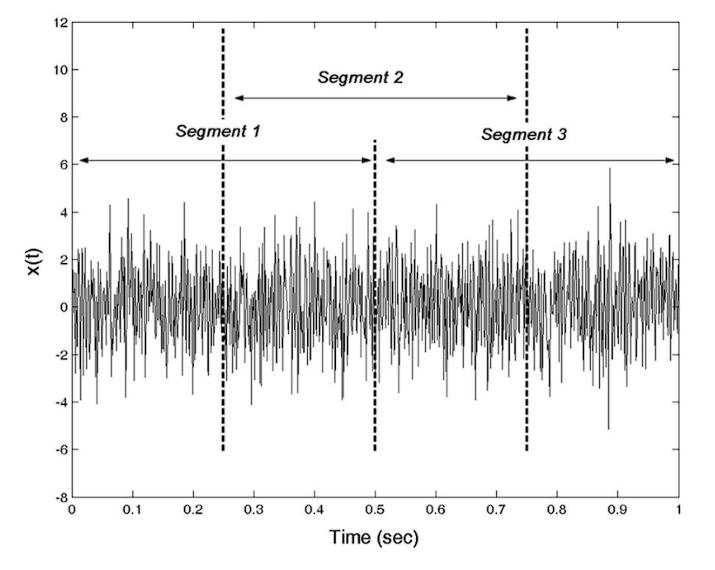
\includegraphics[width=0.4\textwidth]{images/segments}
\end{figure}
\noindent In the general case, this procedure is called \textbf{Welch's method} and consists in the following steps.
\begin{boxdefinition}{Spectral Averaging - Welch's Method}{}
\begin{enumerate}
     \item Take a short segment of the signal of length \texttt{nsamples}. 
     \item Apply a windowing function $win(t)$.
     \item Compute the windowed periodogram $$
     |DFT(win(t)\cdot x(t))|^2
     $$
     and store the resulting PSD.
     \item Shifts \texttt{nsamples} to the right, (or a fraction of this amount, if overlapping segments are desired). 
     \item Repeat the steps 1 to 4 until the end of the signal is reached, having in total \texttt{num\_samples}. 
     \item Average all the PSDs.
\end{enumerate}
\end{boxdefinition}
\noindent The reduction in spectral resolution is determined by the length of the segment\begin{equation}
     \Delta f\propto \frac{1}{\texttt{nsamples}}
\end{equation}
and the variability of the PSD is reduced by a factor $\sqrt{\texttt{num\_samples}}$.
\begin{figure}[H] 
     \centering
     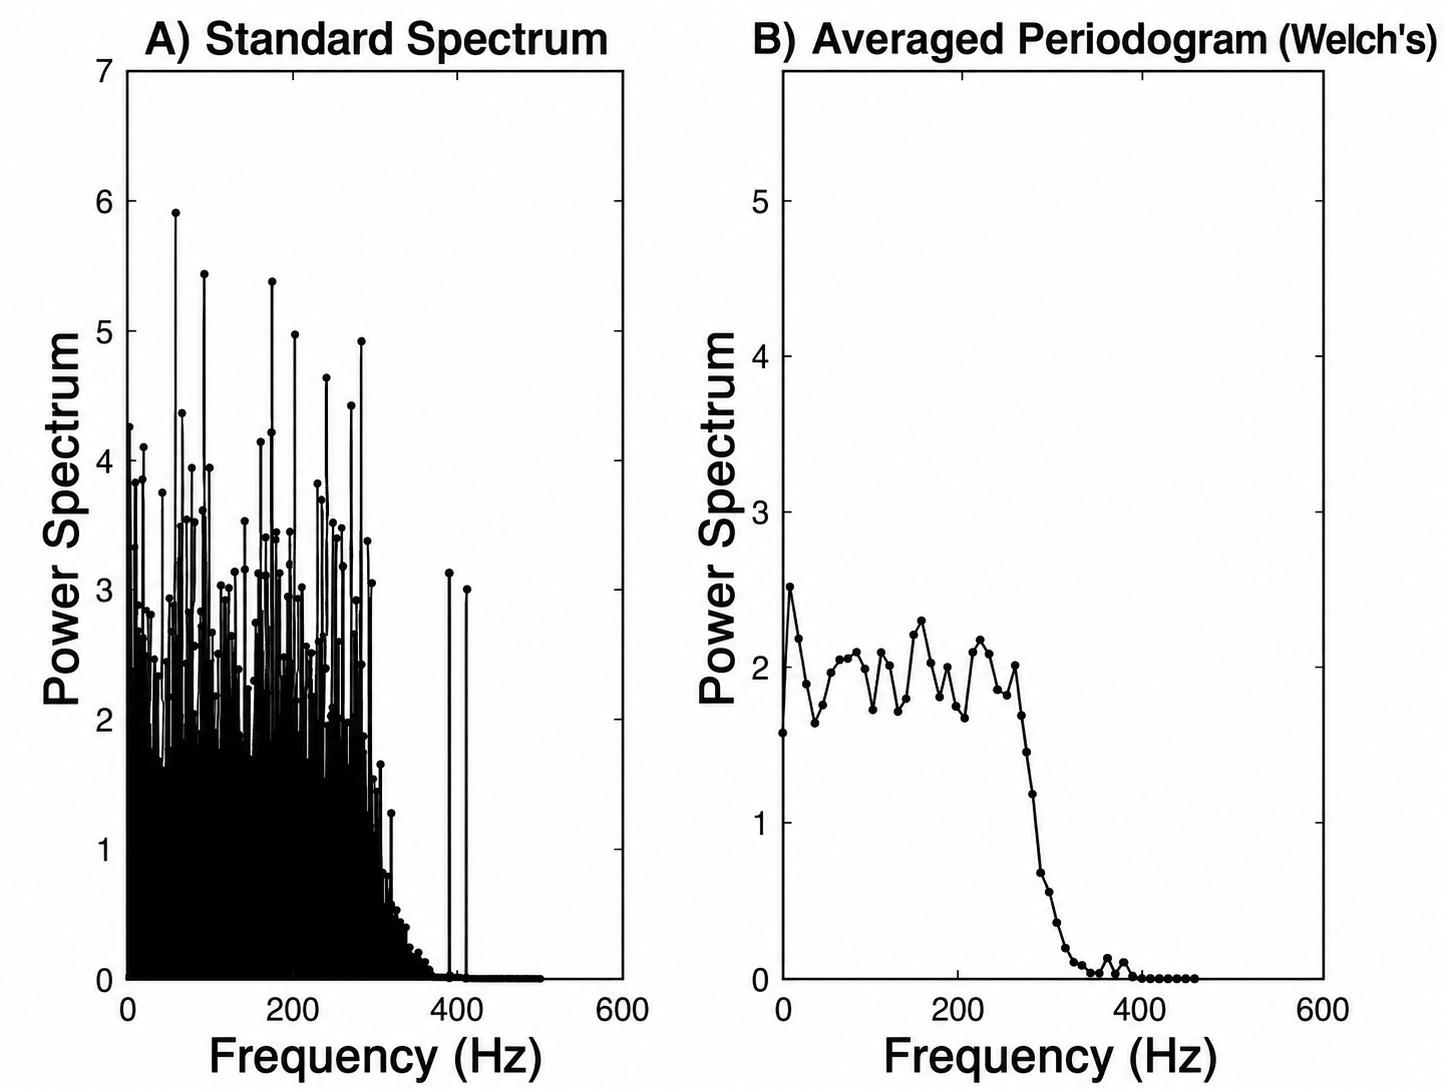
\includegraphics[width=0.45\textwidth]{images/avgPer.png}
     \caption{Averaged periodogram.}
     \label{avgPer}
\end{figure}
In figure \ref{avgPer} we can see the differences between the spectrum computed with the periodogram (left) and the spectrum after the Welch's method (right). \bigskip


\noindent When the signal is \textbf{not stationary}, PSD should not be used to describe the signal's spectrum. If short
segments of the signal can be considered stationary (the signal is pseudo-stationary), the evolution of the
spectrum over time can be displayed using a spectrogram.
\textbf{STFT} (short-time fourier transform) is the simplest method to achieve this goal.
\begin{figure}[H] 
     \centering
     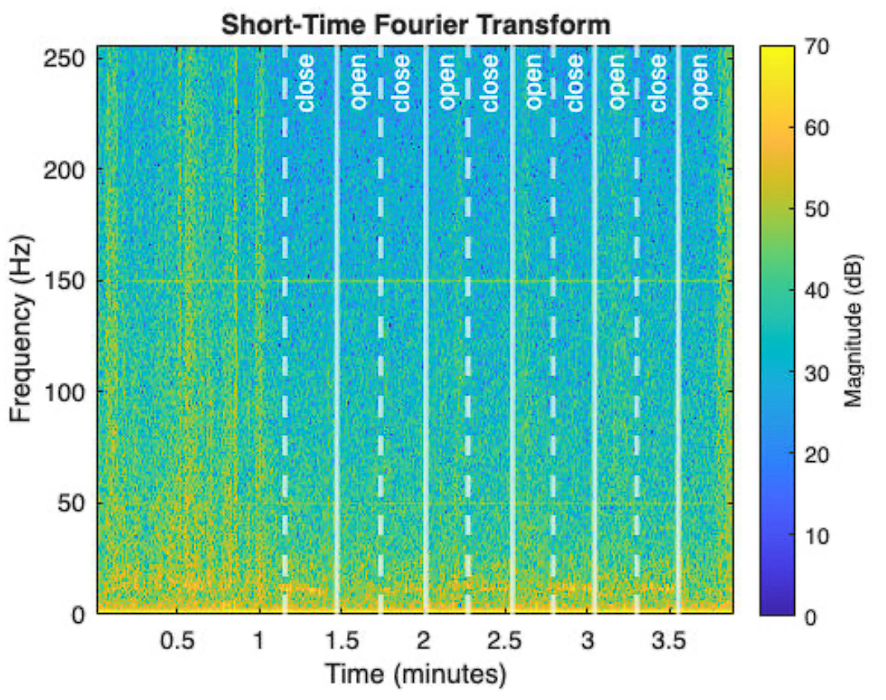
\includegraphics[width=0.5\textwidth]{images/spectrogram.png}
     \caption{Spectrogram.}
\end{figure}
Every vertical bar of this diagram is a spectrum, the spectrum is color coded, for each time window a spectrum is computed.

\section{Digital Filters}
A filter is needed to remove or attenuate some components of the signal that we are acquiring: Usually we divide a signal in two components, the useful information, and the noise/disturbance. Most of the time, signal and noise have almost separate components in the spectrum. Filters are a way to \textit{improve the signal/noise ratio}.

In real filters, the signal passes almost unaltered, and the noise is almost removed (never completely blocked). There are four families of filters, and they differs in how they modify the spectrum of a signal:
\begin{figure}[H] 
     \centering
     
\includegraphics[width=0.55\textwidth]{images/filters.png}
\end{figure}
The passband refers to those frequencies that are passed, while the stopband contains those frequencies
that are blocked. The transition band is between. A fast \textbf{roll-off }means that the transition band is very
narrow.

The division between the passband and transition band is called the \textbf{cutoff frequency}. In analog filter design,
the cutoff frequency is usually defined to be where the amplitude is reduced to 0.707 times the input (i.e. -3dB). Digital filters often specify different attenuation at the cutoff frequency, depending on the synthesis
process.\bigskip

\noindent Let's see three properties that measures how well a filter performs. The first one is the already mentioned roll-off, to separate closely spaced frequencies, the filter must have a fast roll-off:
\begin{figure}[H] 
     \centering
     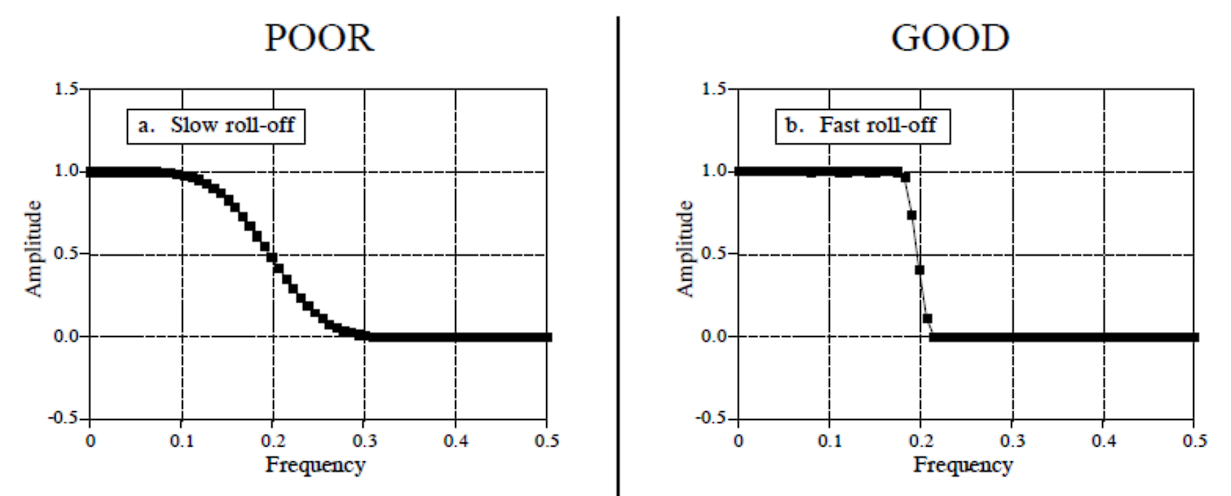
\includegraphics[width=0.7\textwidth]{images/roll_off.png}
\end{figure}
For the passband frequencies to move through the filter unaltered, there must be no passband ripple:
\begin{figure}[H] 
     \centering
     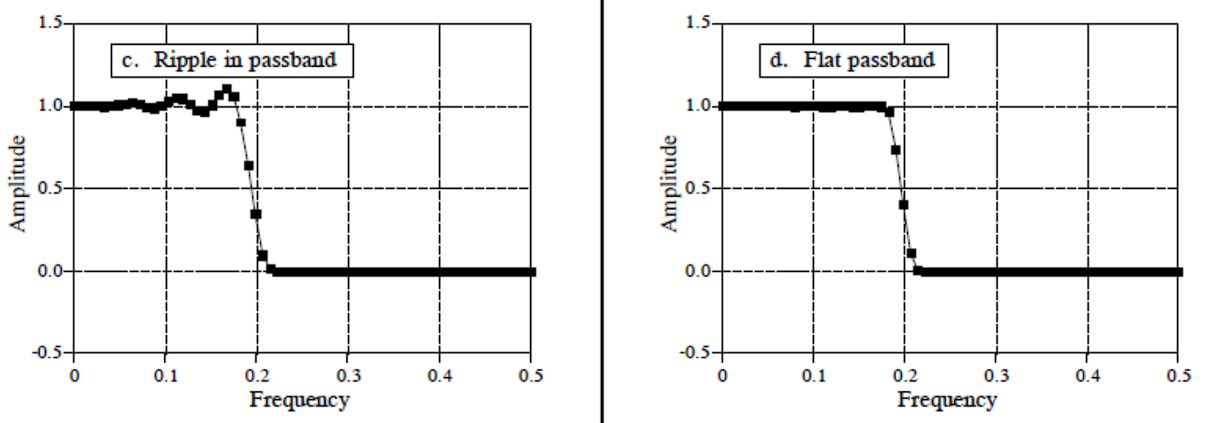
\includegraphics[width=0.7\textwidth]{images/ripple.png}
\end{figure}
\noindent Lastly, to adequately block the stopband frequencies, it is necessary to have good stopband attenuation:
\begin{figure}[H] 
     \centering
     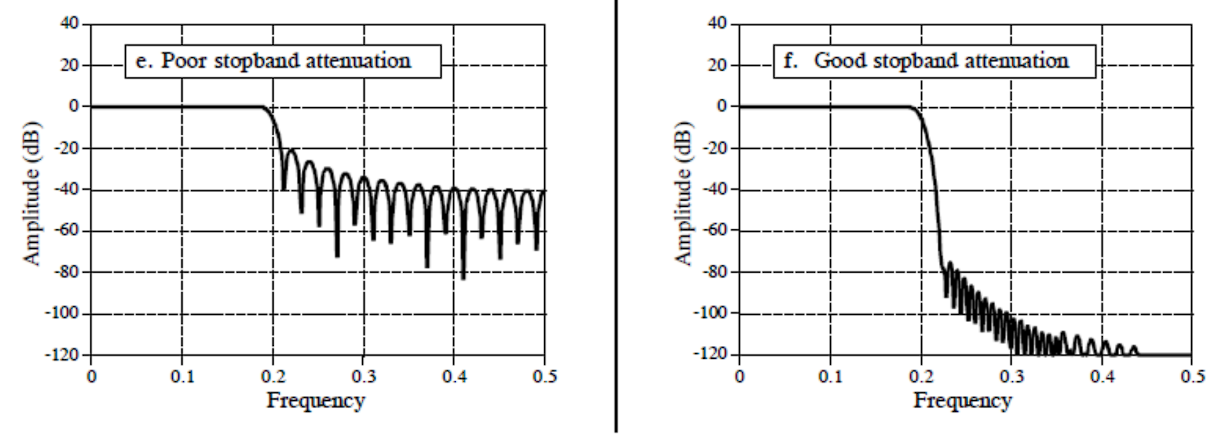
\includegraphics[width=0.7\textwidth]{images/attenuation.png}
\end{figure}
\subsection{FIR and IIR Filters}
We have divided the filters in 4 families, by distinguish them from the band that they attenuate. There is an other different classification in 2 families, \textbf{Finite Input Response (FIR)} and \textbf{Infinite Input Response (IIR)}.\bigskip

FIR filters are systems where the output is calculated based solely on the current and past input values. Because they lack feedback loops, their impulse response eventually hits zero and remains there after a finite number of steps. In FIR filters the output $y[i]$ is computed by combining samples of the input:\begin{equation}
     y[i]=\sum_{k=0}^{N}b_kx[i-k]
\end{equation}
is a weighted sum of the $N$ inputs $x[i],x[i-1]\dots x[i-N]$. The definition of the coefficients $b_k$ defines the behavior of the filter. These filters are not much used in practice. On the other hand, an IIR filter have the output computed by combining samples of the input and previous samples of the output:\begin{equation}
     y[i]=\sum_{k=0}^{M}b_kx[i-k]-\sum_{k=1}^{N}a_ky[i-k].
\end{equation}
The order $\max(N,M)$ of a filter indicates how many recent samples are used to compute the output. 
So, to recap the differences:\begin{itemize}
     \item FIR: we have only the convolutive component of the computation of the output. 
     \item IIR: we have both the convolutive component and a recursive component.
\end{itemize}
Some common design methods for FIR filters are:\begin{itemize}
     \item windowed sinc 
     \item minimax
\end{itemize}
on the other hand, design methods for IIR filters are:\begin{itemize}
     \item Butterworth
     \item Chebyshev (type I or II)
     \item elliptic.
\end{itemize}
An RC filter is the simplest type of an analog Butterworth filter. \bigskip

\noindent\textbf{Example}: The following image shows the difference between a raw signal (blue) and the filtered signal (orange):
\begin{figure}[H] 
     \centering
     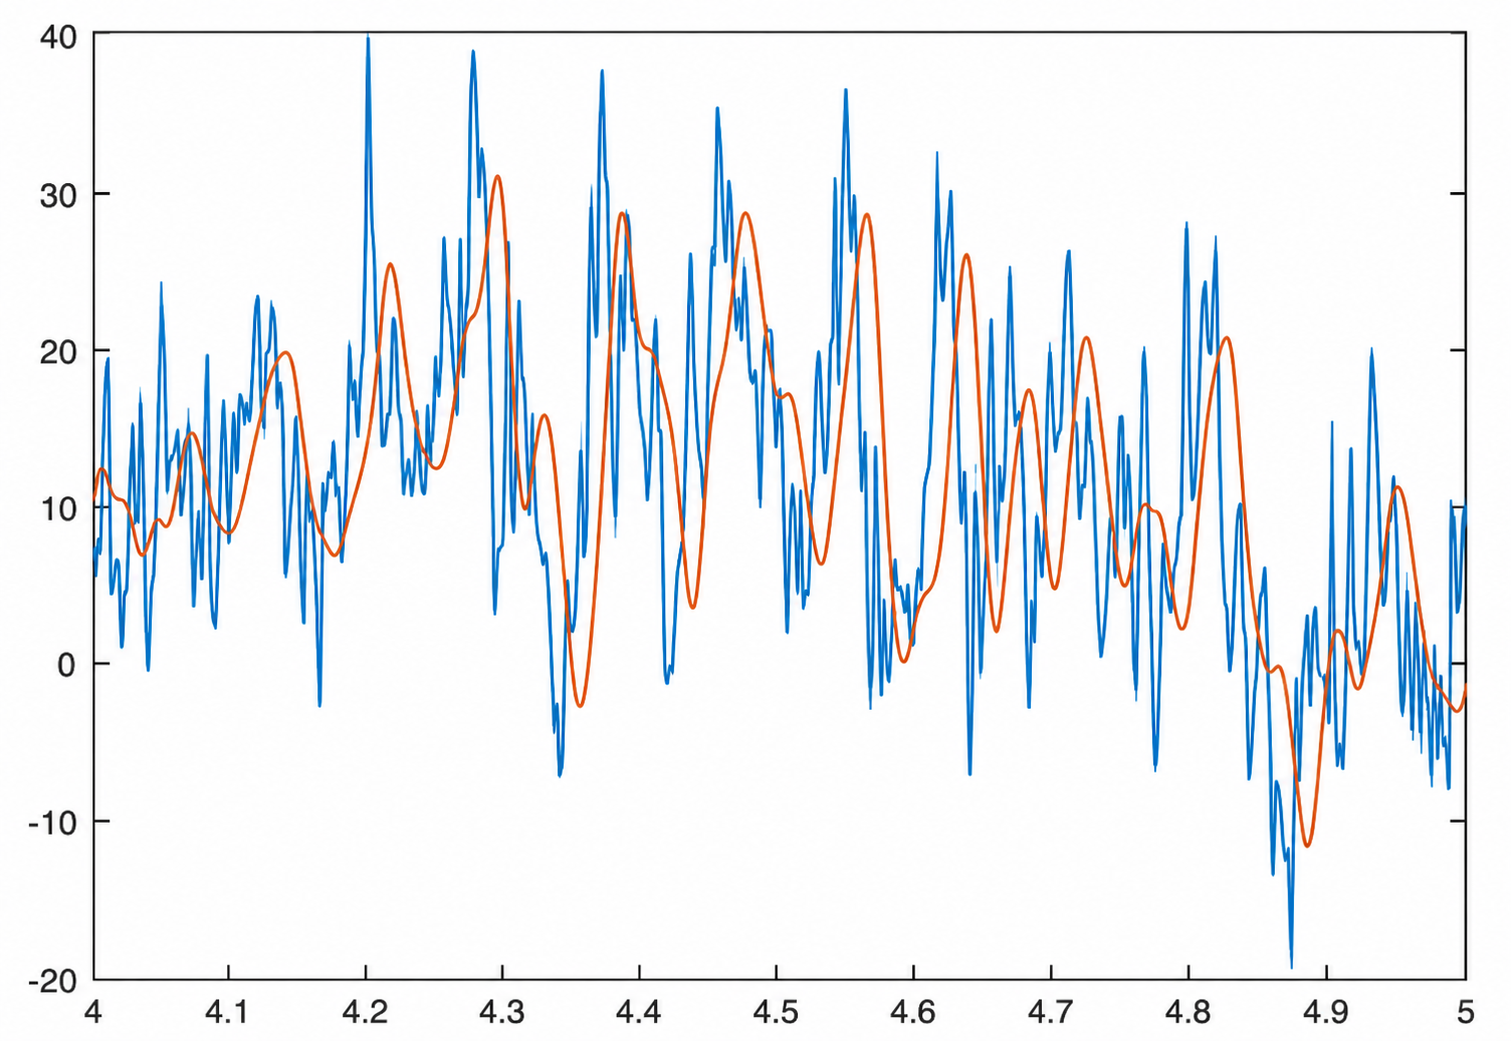
\includegraphics[width=0.5\textwidth]{images/raw_filter.png}
\end{figure}
\noindent We can see how the filter ''smoothed'' the signal, practically reduced the amplitude of the signal, shifted the signal and eliminated (or at least attenuated) it's high frequency components. The orange signal contains less high frequency components. The low frequency components are preserved, as we can see from the signal at a different scale (in a time window of 10 seconds):
\begin{figure}[H] 
     \centering
     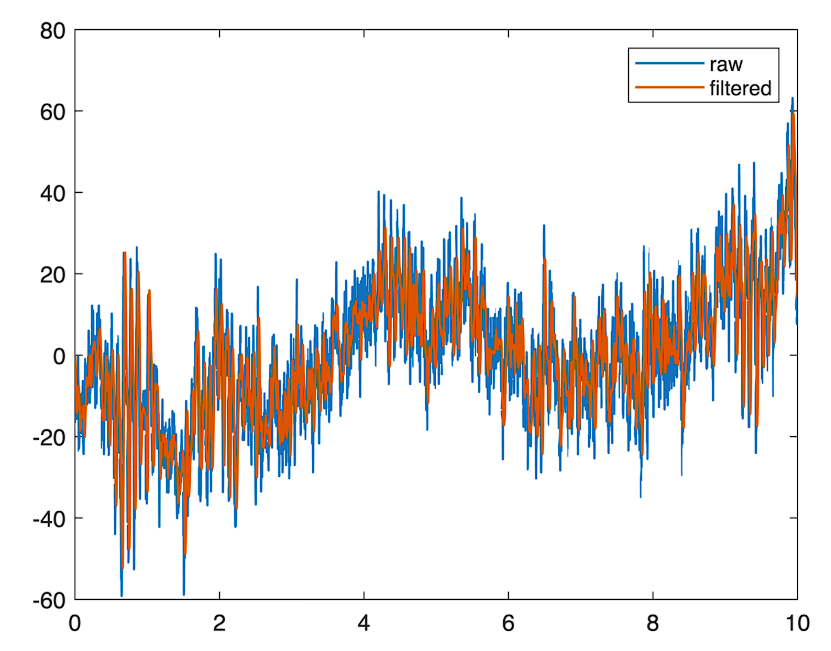
\includegraphics[width=0.5\textwidth]{images/raw_filter2.png}
\end{figure}
\noindent We applied a low-pass filter, the power/frequency plot of the filter is the following:
\begin{figure}[H] 
     \centering
     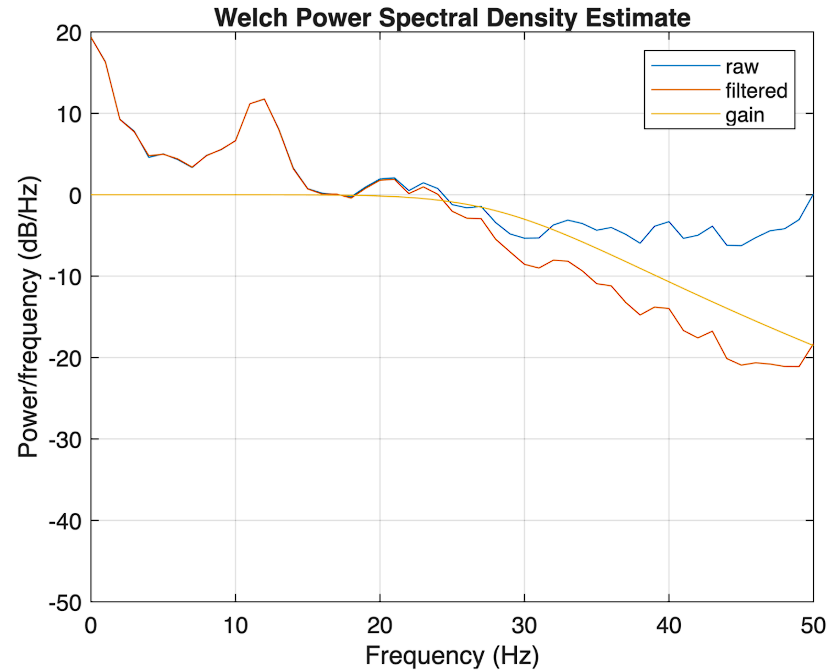
\includegraphics[width=0.5\textwidth]{images/raw_filter3.png}
\end{figure}
\noindent The blue line is the spectrum of the raw signal, the orange one is the spectrum of the filtered one. At the beginning the two signal have the same spectrum, the frequency components of 20 Hz or less are not attenuated. After 30 Hz (cut off frequency) there is a visible difference in attenuation, and the higher the frequency, the higher is the attenuation. 
\chapter{Brain-Computer Interfaces}
\section{What is a Brain--Computer Interface?}

\subsection{Formal Definition}

A Brain--Computer Interface (BCI) is a system that measures signals originating in the
Central Nervous System (CNS) and converts them into an artificial output. The defining
characteristic of a BCI — the feature that distinguishes it from all other human--machine
interfaces — is that it \emph{completely bypasses} the normal nerve and muscle pathways
that humans naturally use to interact with their environment.

\begin{boxdefinition}{BCI}{}
A \textbf{Brain--Computer Interface (BCI)} is a system that measures CNS activity and
converts it into an artificial output that replaces, restores, enhances, supplements, or
improves natural CNS output, without relying on normal neuromuscular pathways.
\end{boxdefinition}

\subsection{The Five Goals of a BCI}

According to the taxonomy established by Wolpaw \& Wolpaw (2012), the artificial output of a
BCI is designed to achieve one of five goals, each corresponding to a distinct clinical or
engineering objective:

\begin{enumerate}
  \item \textbf{Replace.} A permanently lost function is substituted entirely. A classical
  example is a paralysed patient using a BCI to drive a motorised wheelchair or
  communicate via a speller interface.

  \item \textbf{Restore.} A specific lost ability is given back to the user. For instance, a
  BCI may restore the capacity to grasp an object by controlling a robotic prosthesis or
  a functional electrical stimulation (FES) device.

  \item \textbf{Enhance.} An existing cognitive or physiological function is augmented
  beyond its natural baseline. A monitoring system that detects driver drowsiness from
  EEG and triggers an alert exemplifies this category.

  \item \textbf{Supplement.} The BCI adds a new channel of communication or control
  that complements, rather than replaces, the user's natural neuromuscular output.

  \item \textbf{Improve.} The BCI is used to train or rehabilitate a damaged function,
  with the aim of promoting genuine biological recovery.
\end{enumerate}

\subsection{The BCI as a Closed-Loop System}

The translation of neural intent into external action requires the BCI to operate as a
\textbf{closed-loop pipeline}. Critically, this loop is not merely a technical convenience; it
is a \emph{physiological necessity}. Because controlling a device through brain signals is
an entirely unnatural skill, the user's brain requires continuous real-time feedback to
evaluate its own performance, detect errors, and progressively refine the generated signals.
This process is directly analogous to learning any new motor skill — such as playing tennis
or riding a bicycle — where the absence of feedback would render learning impossible.

The pipeline consists of four sequential stages:

\begin{enumerate}
  \item \textbf{Intention (User Training).} The user performs a specific cognitive task —
  such as imagining a movement or attending to a stimulus — in order to generate a
  predictable, detectable modification in their brain signals.

  \item \textbf{Extraction.} Signal-processing algorithms operate on the raw acquired
  signal to isolate and quantify the relevant features (e.g., the amplitude of a specific
  frequency component, or the magnitude of an event-related potential).

  \item \textbf{Translation (Classification).} The extracted features are fed into a
  classification or regression algorithm that maps them onto a discrete or continuous
  control command.

  \item \textbf{Command and Feedback.} The decoded command is executed in the
  external environment. The resulting outcome is presented back to the user as sensory
  feedback, closing the loop and enabling the brain to adapt iteratively.
\end{enumerate}

\begin{boxobservation}{}{}
Real-time feedback is not optional in a BCI system — it is a fundamental component of
the architecture. Without it, the closed-loop mechanism collapses and effective user
learning cannot occur.
\end{boxobservation}

\subsection{Signal Acquisition Methods}

Brain signals can be acquired through two broad categories of methods, which differ
substantially in their invasiveness, spatial resolution, temporal resolution, and practical
applicability:

\begin{itemize}
  \item \textbf{Implanted (invasive) methods.} Sensors are surgically positioned on or
  within the brain tissue. Examples include Electrocorticography (ECoG) grids placed
  directly on the cortical surface, and microelectrode arrays that record Local Field
  Potentials (LFP) or single-/multi-unit spiking activity (SUA/MUA). These methods
  offer excellent spatial resolution and signal quality but carry the inherent risks
  associated with neurosurgical procedures.

  \item \textbf{Non-implanted (non-invasive) methods.} Sensors are placed externally on
  the scalp. Several modalities exist, including Functional Magnetic Resonance Imaging
  (fMRI) and Near-Infrared Spectroscopy (NIRS). However, \textbf{Electroencephalography
  (EEG)} remains by far the most widely used and extensively studied technique for
  non-invasive BCIs, primarily due to its high temporal resolution, relatively low cost,
  and portability.
\end{itemize}

\subsection{Two Primary Clinical Paradigms}

In clinical practice, non-invasive BCI systems are deployed under two overarching
paradigms, which form the structural backbone of these notes:

\begin{itemize}
  \item \textbf{Assistive BCIs} substitute a permanently lost function — most commonly
  communication or environmental (domotic) control — by routing decoded brain signals
  into commercial assistive technology software.

  \item \textbf{Rehabilitative BCIs} harness the brain's own plasticity to drive the
  biological recovery of a damaged function, rather than merely bypassing it.
\end{itemize}

\section{The Accessibility Gap in Assistive Technology}

\subsection{Rethinking Disability}

In the context of Assistive Technology (AT), disability is not conceived as an intrinsic medical
deficiency of the individual. Rather, guided by the World Health Organization's framework,
disability is understood as a \textbf{mismatch between a person's condition and their
environment}. Assistive Technology functions as the bridge that closes this gap, encompassing
any device, software, or system that enables individuals to perform tasks they would
otherwise be unable to do. The primary goals of AT are the restoration of autonomy, dignity,
meaningful social participation, and effective communication.

\subsection{The Fundamental Limitation of Conventional AT}

Conventional digital AT solutions — including joysticks, touch screens, computer mice, head
trackers, and eye-tracking devices — are highly capable interfaces. However, they all share
one fundamental constraint: they require the user to produce a \emph{reliable, voluntary
muscular or physical movement} to generate a command. Even an eye-tracking device, which
might appear to require no effort, demands intact oculomotor control.

When a severe neurological condition — such as Amyotrophic Lateral Sclerosis (ALS),
Locked-In Syndrome (LIS), or a severe stroke — compromises all residual motor function,
every one of these solutions becomes inaccessible simultaneously. This is the
\textbf{accessibility gap} that BCIs are uniquely positioned to address.

By bypassing the neuromuscular system entirely and using brain-derived signals as the
control channel, BCIs provide access to digital environments even when no reliable physical
movement remains.

% ============================================================
\section{The P300 Event-Related Potential}

\subsection{Event-Related Potentials and the P300}

Non-invasive BCIs based on EEG frequently exploit \textbf{Event-Related Potentials (ERPs)}:
transient voltage deflections in the EEG that are time-locked to the presentation of a specific
stimulus. Because ERPs are typically smaller in amplitude than the ongoing background EEG,
they are extracted by \textbf{signal averaging}: the EEG epochs following repeated stimulus
presentations are aligned and averaged across trials, causing random background noise to
cancel out while the consistent, stimulus-locked response is preserved.

The most prominent ERP exploited in assistive BCIs is the \textbf{P300 wave}:

\begin{boxdefinition}{The P300 Wave}{}
The P300 is a large, positive voltage deflection in the EEG occurring approximately
\textbf{300~ms} after the presentation of a target stimulus. It is most pronounced over
the \textbf{centro-parietal} scalp regions and is physiologically associated with higher
cognitive processes including memory updating, attentional allocation, and executive
function.
\end{boxdefinition}

\subsection{The Oddball Paradigm}

The P300 is reliably elicited using the \textbf{oddball paradigm}, a classic psychophysical
protocol. A stream of stimuli is presented to the user, consisting of:

\begin{itemize}
  \item \textbf{Frequent, non-target stimuli}: common events that the user is instructed
  to ignore;
  \item \textbf{Rare, target stimuli}: infrequent, task-relevant events that the user is
  instructed to attend to.
\end{itemize}

Because the P300 is a neural response to \emph{rare, meaningful events}, it is generated
exclusively when the user's attended target stimulus is presented. Non-target stimuli do
not elicit this response. This selectivity is the key property that makes the P300 useful as
a BCI control signal.

\subsection{The P300 Speller Matrix}

The classical implementation of the P300 oddball paradigm in the context of assistive
communication is the \textbf{P300 Speller}, originally developed by Farwell \& Donchin (1988).
The interface presents the user with a matrix of characters — typically a 6$\times$6 grid of
letters, numbers, and symbols. The rows and columns of the matrix flash in a randomised
sequence.

The operating principle is as follows:
\begin{enumerate}
  \item The user fixates their attention on the desired character (the \emph{target}).
  \item As rows and columns flash randomly, the P300 response is elicited \emph{only}
  when the row or column containing the target character is illuminated.
  \item Flashes of all other rows and columns do not elicit the P300.
  \item After accumulating a sufficient number of flashes (to improve the signal-to-noise
  ratio through averaging), the system identifies which row and which column elicited the
  P300 response. Their intersection corresponds to the intended character.
\end{enumerate}
\section{BCI as a Modular AT Channel}

\subsection{Integration Over Reinvention}

Historically, BCI research tended to produce \emph{standalone}, monolithic systems: the
BCI software managed not only the signal processing and classification, but also the entire
application layer (e.g., a dedicated spelling program). This approach was pragmatically
limiting, as it required researchers to perpetually reinvent sophisticated software
functionality — word processors, communication aids, web browsers — that already existed
in highly refined commercial forms.

The contemporary paradigm in neuroengineering prioritises \textbf{integration over
reinvention}. The modern BCI is designed to act exclusively as an \textbf{alternative access
channel}, sitting at the exact same hierarchical level as a conventional input device (mouse,
joystick, head tracker, etc.). The classification output is a generic, hardware-agnostic
``selection'' event that any compatible AT platform can interpret.

\subsection{Technology Readiness and the Clinical Pipeline}

This architectural shift carries important implications for clinical translation. The transition
from isolated laboratory prototypes (Technology Readiness Level, TRL~4) to modular,
commercially deployable systems (TRL~7--8) is a critical milestone. Systems such as
BCI2000 handle the stimulation and classification stages and pass a discrete
\emph{Selection} trigger to platforms like GRID3, which drive the end-user application.
This modularity makes the system far easier to validate, maintain, and deploy in real
clinical and domestic settings.

\begin{boxobservation}{}{}
The modular AT approach is not merely a software engineering convenience. It is a
prerequisite for clinical viability: only by leveraging mature commercial AT platforms can a
BCI achieve the functional breadth and reliability required for everyday use by people with
severe motor impairments.
\end{boxobservation}


\section{Physiological Foundations of Rehabilitative BCIs}

Rehabilitative BCIs serve a fundamentally different purpose from their assistive
counterparts. Rather than \emph{substituting} a permanently lost function by routing around
the damaged neuromuscular system, a rehabilitative BCI aims to \emph{restore} the
impaired biological function itself. In the context of stroke recovery, the BCI acts as a
temporary neuro-technological driver: by engaging the damaged motor networks in a
precisely structured way, the system actively guides Central Nervous System (CNS)
plasticity, with the goal of facilitating the progressive recovery of voluntary movement.

\subsection{Neuroplasticity and Its Role in Recovery}

The CNS is not a static organ. It possesses a remarkable intrinsic capacity to reorganise
its neural connections in response to experience, learning, and injury — a property
collectively referred to as \textbf{neural plasticity}. Following a stroke, surviving perilesional
tissue and contralateral homologous areas can, under appropriate conditions, assume some
of the functions formerly carried out by the damaged region.

Rehabilitative BCIs capitalise on this plasticity by creating a highly structured training
environment that drives the brain to explore and consolidate new neural strategies for
motor control.

\subsection{Motor Imagery as the Physiological Interface}

A central challenge in rehabilitation is that severely paretic or plegic patients cannot
produce overt movements. How, then, can the motor network be engaged? The solution lies
in \textbf{Motor Imagery (MI)}: the deliberate mental rehearsal of a movement without any
associated muscular activation.

Neuroimaging studies have demonstrated that the cortical networks recruited during MI
overlap substantially with those activated during actual movement execution, including the
\textbf{primary motor cortex (M1)}, the \textbf{supplementary motor area (SMA)}, and the
\textbf{premotor cortex}. This functional equivalence makes MI a valid
and detectable proxy for motor intent, even when the descending neuromuscular pathways
are severed or damaged.

\begin{boxobservation}{}{}
Kinesthetic motor imagery — in which the patient mentally rehearses the internal
sensation and muscular effort of movement from a first-person perspective — is
substantially more effective at recruiting the motor network than visual motor imagery (in
which the patient imagines \emph{watching} themselves move from a third-person
viewpoint). The latter engages primarily visual processing areas and generates insufficient
SMR modulation for effective BCI control.
\end{boxobservation}

\subsection{Sensorimotor Rhythms and Event-Related Desynchronisation}

Non-invasive rehabilitative BCIs detect motor intent by monitoring continuous EEG
oscillations known as \textbf{Sensorimotor Rhythms (SMR)}. These oscillations are
recorded over the sensorimotor cortex and are concentrated primarily in the \textbf{mu
band} (8--12~Hz) and the \textbf{beta band} (14--30~Hz).

The functional behaviour of the SMR is directly analogous to the well-known \emph{alpha
block} phenomenon in the visual cortex:
\begin{itemize}
  \item During \textbf{motor rest}, the sensorimotor neuronal populations are
  synchronised, producing a high-amplitude, regular oscillation in the mu and beta bands.
  \item During \textbf{movement or motor imagery}, the neuronal populations rapidly
  desynchronise to process the complex motor command, causing a pronounced
  \emph{decrease} in the amplitude and spectral power of the SMR.
\end{itemize}

This power decrease is formally termed \textbf{Event-Related Desynchronisation (ERD)}.
In an asynchronous rehabilitative BCI, the system continuously monitors the SMR power
spectrum in real time; a quantified drop in power below a resting baseline is classified as
evidence of active motor intention.

\begin{boxobservation}{}{}
The term \emph{ERD} has a precise technical definition: it refers to a non-stationary
spectral change that must be estimated by averaging across multiple trials time-locked to
a discrete triggering event. However, in the BCI literature — and in informal communication
among researchers — the term is frequently used as a generic synonym for \emph{any}
drop in SMR power, including during continuous, asynchronous state classification (i.e.,
in the absence of a discrete event). As neuroengineers, you should be aware of this
semantic overextension and interpret the term according to its context.
\end{boxobservation}

% ============================================================

\section{System Architecture: Driving Neuroplasticity}

\subsection{Closing the Broken Sensorimotor Loop}

In stroke patients with severe motor impairment, the descending neural pathways —
particularly the corticospinal tract — are disrupted, effectively severing the connection
between the motor cortex and the peripheral muscles. This disconnection creates a vicious
cycle: the inability to move deprives the motor cortex of the sensory feedback that
movement would normally generate, thereby inhibiting the plasticity required for recovery.

Rehabilitative BCIs intervene precisely at this point. Rather than controlling a screen
cursor, the regression score derived from real-time SMR modulation is used to command a
\textbf{physical assistive device} coupled to the patient's paretic limb — either a
robotic exoskeleton or a \textbf{Functional Electrical Stimulation (FES)} device. When
the patient performs kinesthetic motor imagery and the BCI detects the corresponding
cortical signal, it triggers the device to execute the imagined movement.

\subsection{Endogenous vs. Exogenous Drivers}

Neuroplasticity-enhancing interventions can be classified according to what drives neural
reorganisation:

\begin{itemize}
  \item \textbf{Exogenous drivers} rely on \emph{external} interventions to promote
  connectivity changes. Examples include passive robotic mobilisation, Transcranial
  Magnetic Stimulation (TMS), and Transcranial Direct Current Stimulation (tDCS).

  \item \textbf{Endogenous drivers} require the patient's \emph{active, internal} neural
  participation. Motor Imagery-based BCIs are the prototypical endogenous driver: the
  therapeutic input is triggered by, and contingent upon, the patient's own decoded
  motor intent.
\end{itemize}

The clinical significance of BCI-FES or BCI-robot systems lies precisely in this
combination: an \emph{endogenous} decoder commands what is physically an
\emph{exogenous} device, creating a maximally contingent sensorimotor loop.

\subsection{Contingent Sensory Feedback and Hebbian Plasticity}

The ultimate therapeutic mechanism is not the movement of the device itself, but the
\textbf{sensory feedback} that the movement generates. When the exoskeleton opens the
patient's paralysed hand, proprioceptive signals from muscles and joints, together with
cutaneous tactile information, are relayed to the \textbf{primary somatosensory cortex
(S1)}. Simultaneously, visual feedback from watching the hand open is processed by the
visual cortex.

Crucially, the BCI ensures that this rich sensory input arrives at the exact moment the
motor cortex is engaged in imagining the movement. This precise temporal coincidence
between motor output (cortical intent) and somatosensory input (peripheral feedback)
instantiates the classical \textbf{Hebbian learning} principle — ``neurons that fire together,
wire together'' — reinforcing the surviving neural pathways and guiding the CNS to
reorganise around the lesion.

% ============================================================
\section{Advanced Architectures: Hybrid BCIs and Corticomuscular Coherence \textnormal{\small(Optional)}}

As rehabilitative BCIs mature, researchers are exploring more sophisticated hybrid
architectures that monitor neural activity at multiple levels of the motor system
simultaneously.

\subsection{The Concept of Corticomuscular Coherence}

\textbf{Corticomuscular Coherence (CMC)} quantifies the degree of functional
synchronisation between cortical motor commands (measured via EEG) and the resulting
peripheral muscle activation (measured via EMG). A traditional rehabilitative BCI monitors
only the brain signal; a CMC-based hybrid BCI monitors \emph{both} levels and decodes the
integrity of the full corticospinal communication pathway.

\subsection{Preventing Maladaptive Plasticity}

The critical clinical motivation for CMC-BCI systems is the prevention of
\textbf{maladaptive compensatory strategies}. During stroke recovery, patients often
develop compensatory movement habits — for example, recruiting proximal shoulder
muscles to partially substitute for lost distal hand function, or involuntarily activating the
contralateral healthy limb in a mirror movement. While such strategies may appear
superficially functional, they can actually inhibit the recovery of the correct motor
pathways if reinforced during training.

A CMC-BCI is calibrated to:
\begin{itemize}
  \item \textbf{Encourage} the correct cortical-peripheral coupling: coherent activation
  between the motor cortex and the target muscle group (e.g., finger extensors).
  \item \textbf{Discourage} maladaptive patterns: proximal compensatory recruitment or
  mirror movements in the healthy limb.
\end{itemize}

Only when the system detects the correct, targeted physiological attempt does it trigger
the FES device. This strict gating mechanism aims to enforce an error-free rehabilitation
loop, providing the brain with precisely the sensory feedback that reinforces the desired
motor pathway.

% ============================================================
\section{Clinical Efficacy and Neural Network Reconfiguration}

\subsection{Randomised Controlled Trial Evidence}

The clinical efficacy of the rehabilitative BCI architecture has been evaluated in a
\textbf{randomised controlled trial (RCT)} conducted at Fondazione Santa Lucia (Rome).
Stroke patients were assigned either to a BCI-supported motor imagery training group or
to a control group performing identical motor imagery exercises without BCI-derived
feedback.

Clinical outcomes were assessed using standardised tools: the \textbf{Fugl-Meyer
Assessment (FMA)}, the \textbf{Medical Research Council (MRC) scale}, and the NIH
Stroke Scale (NIHSS). At the conclusion of the one-month training protocol, the BCI group
demonstrated significantly greater functional improvement. Most notably, the probability of
achieving the \textbf{Minimal Clinically Important Difference (MCID)} — the threshold
beyond which the patient perceives a meaningful functional improvement — was
\textbf{2.5 times higher} in the BCI group than in the control group.

\subsection{Evidence of Targeted Neuroplasticity}

Beyond the overt clinical gains, EEG analysis revealed measurable reorganisation of
motor brain networks in the BCI group:

\begin{enumerate}
  \item \textbf{Ipsilesional motor re-engagement.} Topographical maps showed
  significantly greater involvement of the \emph{ipsilesional} (affected-side)
  sensorimotor areas during motor imagery post-training in the BCI group. Furthermore,
  this increase in affected-hemisphere spectral power positively correlated with each
  patient's individual FMA improvement.

  \item \textbf{Motor-specific interhemispheric connectivity.} Analysis of
  \emph{interhemispheric} functional connectivity revealed that the BCI group exhibited
  significantly enhanced coupling between the two hemispheres specifically in the
  \textbf{beta$_1$ and beta$_2$} bands — frequency bands directly associated with motor
  function. In contrast, the control group showed increased connectivity only in the
  theta and alpha bands, which reflect general attentional and cognitive engagement rather
  than motor-specific processing.
\end{enumerate}

These findings provide concrete neurophysiological evidence that the contingent
sensorimotor loop implemented by the BCI actively drives \emph{targeted} motor
neuroplasticity, rather than merely improving general engagement or attention.
\chapter{Electromyography}
The electromyography is the electrical activity generated by the muscles. The following picture shows a recorded electromyography:
\begin{figure}[H]
     \centering
     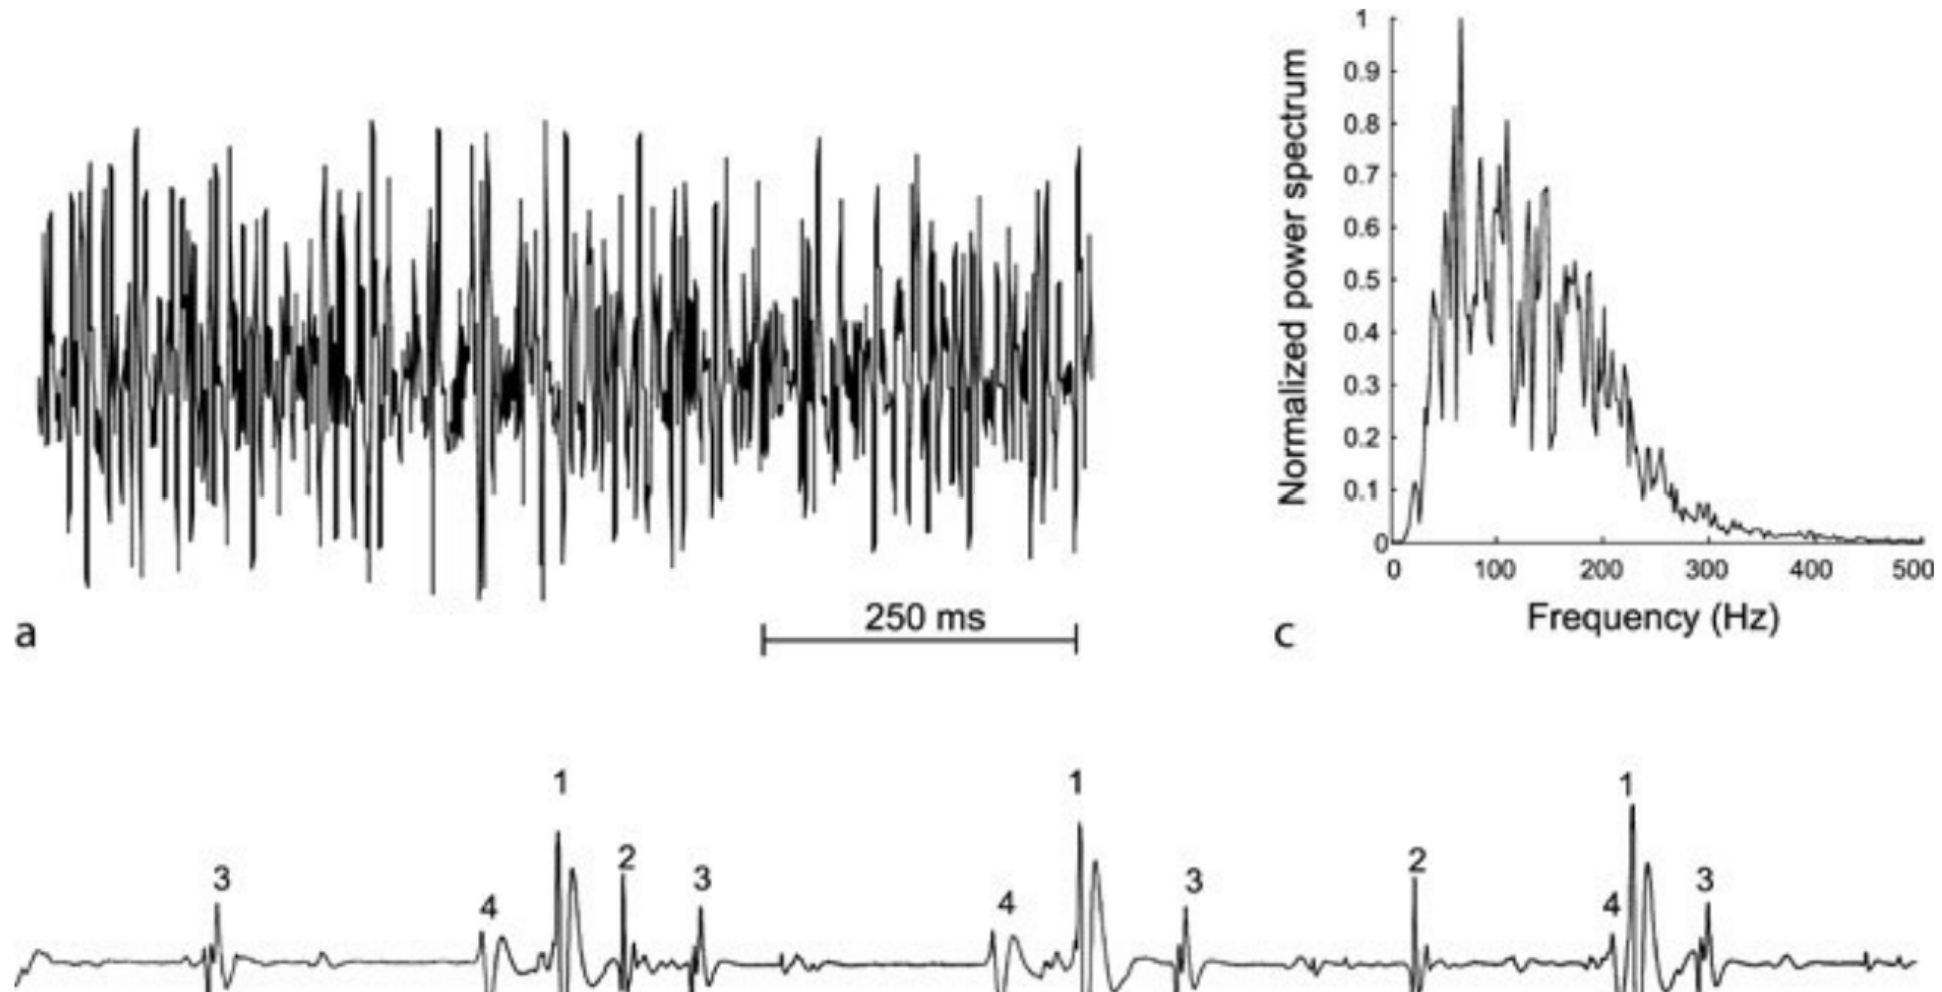
\includegraphics[width=0.6\textwidth]{images/electromyography.png}
\end{figure}
taken with electrodes placed on the skin. Compared to the EEG is faster (presents higher frequency components), the spectrum has frequency components up to (around) 450 Hz. In the EEG, like for the alpha rythm, must of the power is concentrated in the alpha band, no higher than 70 Hz. In the bottom profile of the figure we can see a time zoom of the signal, that comprends a few milliseconds, we observe wavelets of signals, alternating with silence, we can distinguish families of wavelets (labeld with numbers in the picture). \bigskip

There are several application for the electromyography (especially with needle electrodes): 
\begin{figure}[H]
     \centering
     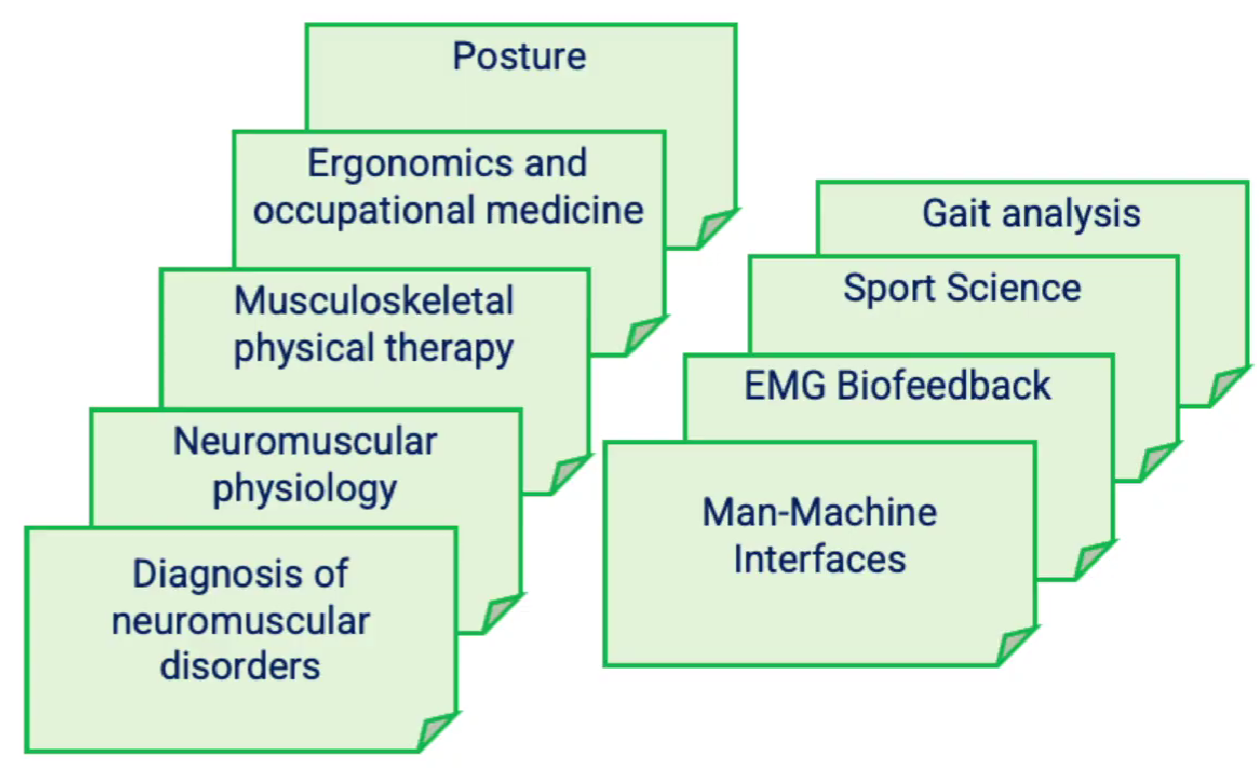
\includegraphics[width=0.4\textwidth]{images/application_electromyography.png}
\end{figure}
\section{Muscle Fibers}
Inside the muscle there are several fascicles, and inside a fascicles there are several muscle fibers.
\begin{figure}[H]
     \centering
     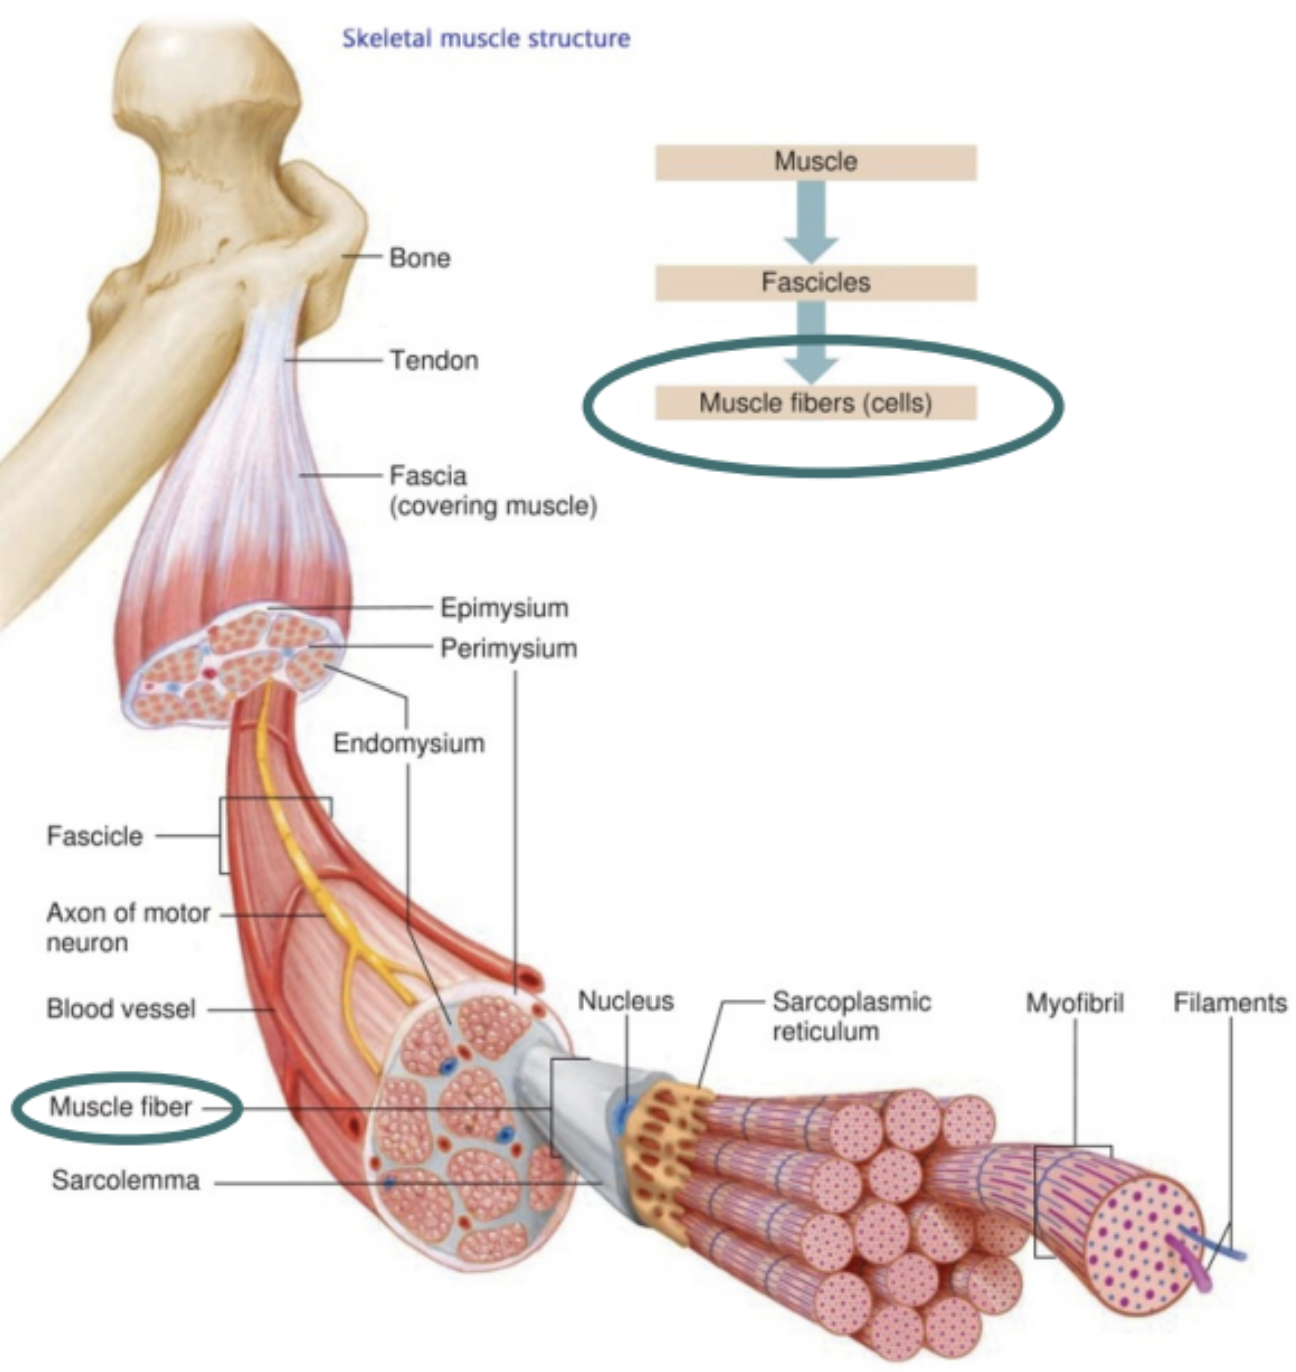
\includegraphics[width=0.4\textwidth]{images/muscle_fiber.png}
\end{figure}
These are the same role that the neurons have for the EEG, they are the core component that generates electrical activity. A single muscle fiber can be in a resting condition, or can produce a response called \textbf{muscle fiber action potential}.
\begin{figure}[H]
     \centering
     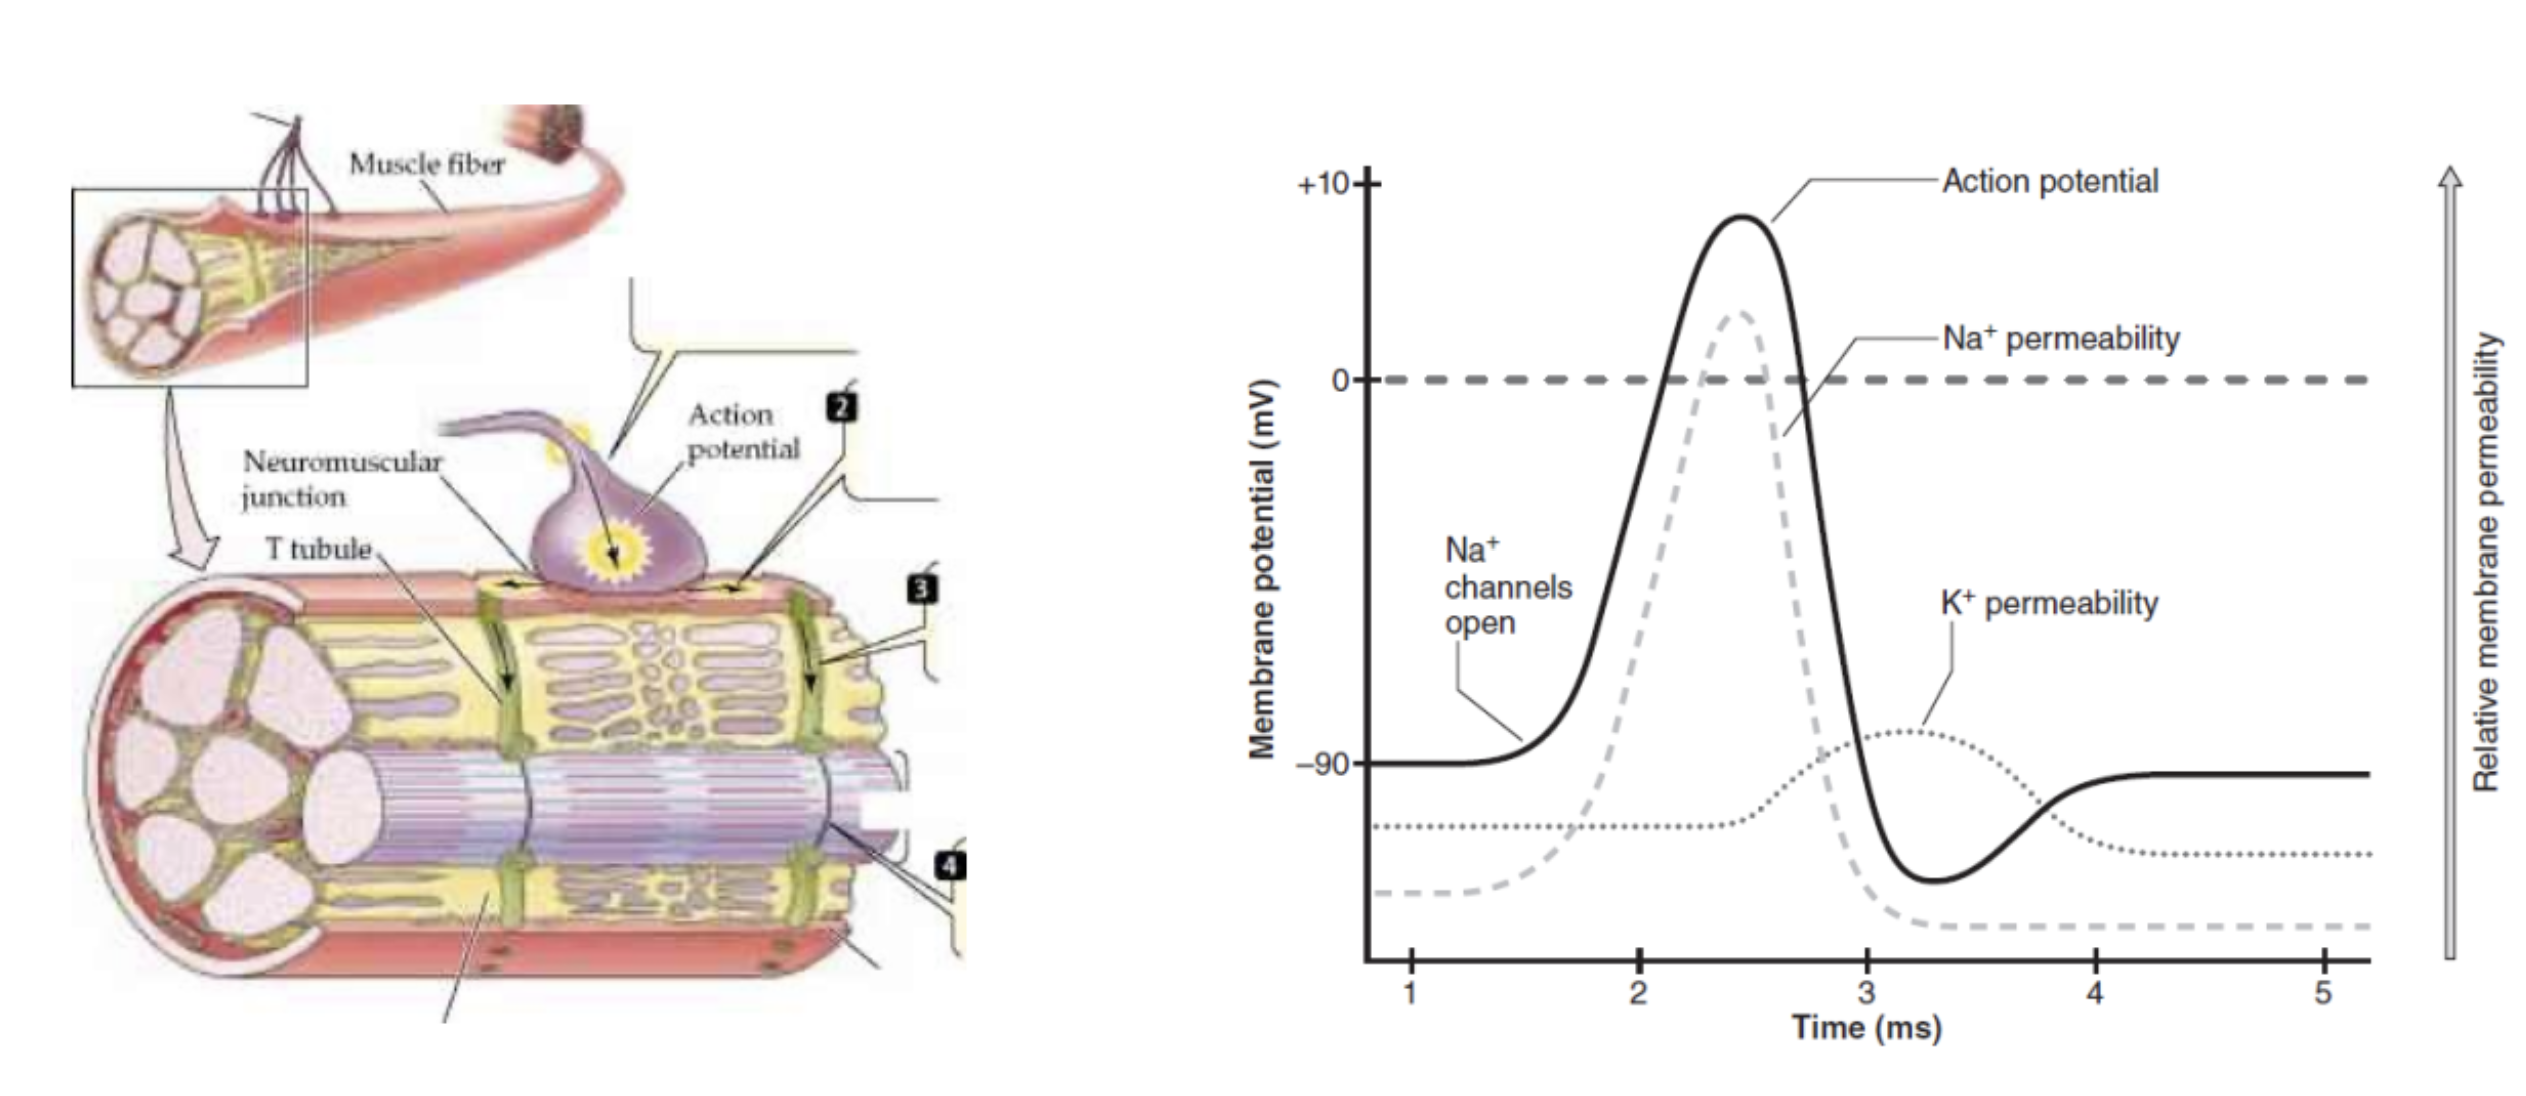
\includegraphics[width=0.8\textwidth]{images/muscle_AP.png}
\end{figure}
The equilibrium is around -90 mV, the action potential touches its peak at around 10 mV. An action potential moves along the muscles, the velocity of movement is called \textbf{Muscle Fiber Conduction Velocity (MFCV)}. The range of this velocity is from 2 to 6 $\frac{\text{m}}{\text{s}}$ and it depends on various factors:\begin{itemize}
     \item ionic concentration,
     \item temperature,
     \item muscle fiber diameter and morphology, 
     \item muscle fiber length,
     \item fiber type,
     \item muscle fatigue (happens because the chemical ions becomes unbalanced),
     \item neuromuscolar pathology.
\end{itemize}
How does the muscle contracts? As for the neurons there is a ''synapse'', is not a synapse between two neurons but between two hetrogeneus cells, one from the nervous system and the other from the muscle system.
\begin{figure}[H]
     \centering
     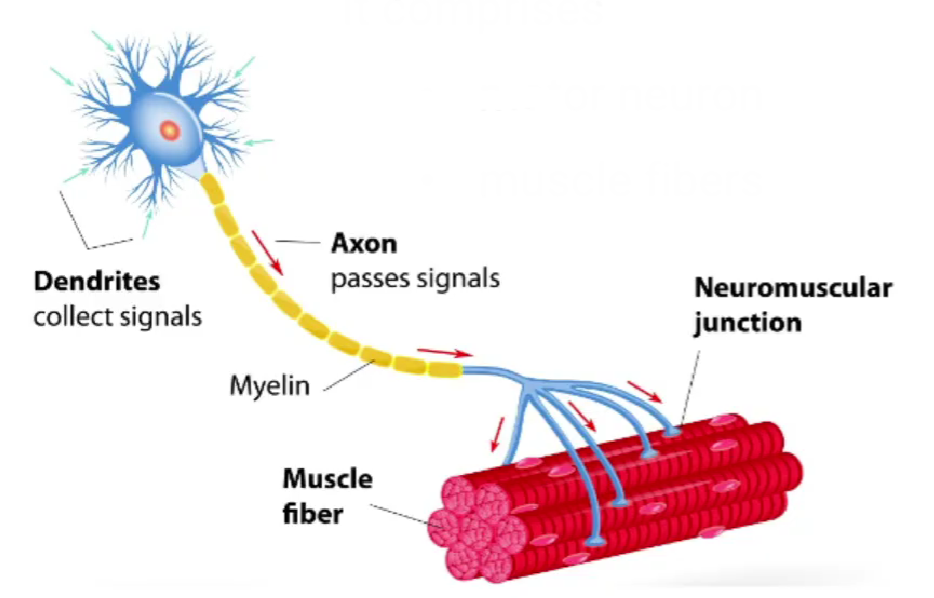
\includegraphics[width=0.55\textwidth]{images/muscle_synapse.png}
\end{figure}
These kind of synapses (they are not really synapses, but acts like them) are called \textbf{neuromuscolar junctions}. They connect one neuron to one fiber, neurons that connects to muscles are called \textit{motor neurons}, one neuron connect to several fibers. A \textbf{motor unit} is one motor neuron with all the fibers connected to it.
\begin{figure}[H]
     \centering
     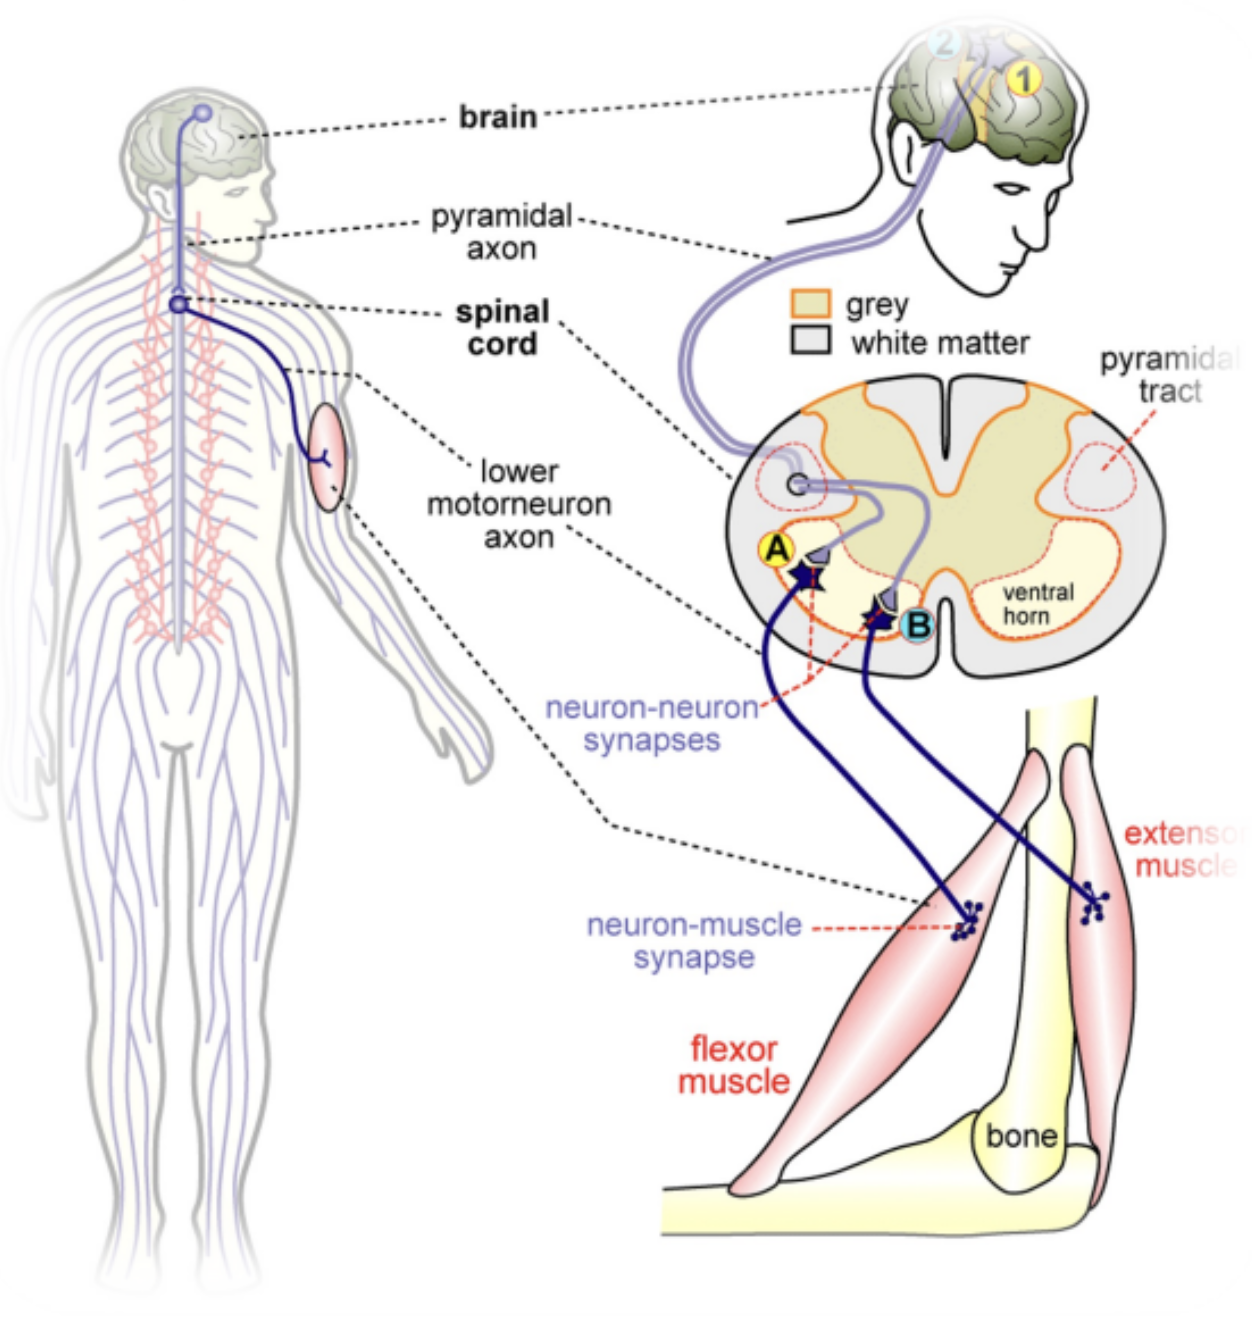
\includegraphics[width=0.35\textwidth]{images/motorNeuron.png}
\end{figure}
Let's focus on a single motor unit, let's say that we have two motor neurons $A$ and $B$, neuron $A$ is connected to fiber 1,4 and 5, neuron $B$ to 2 and 3.
\begin{figure}[H]
     \centering
     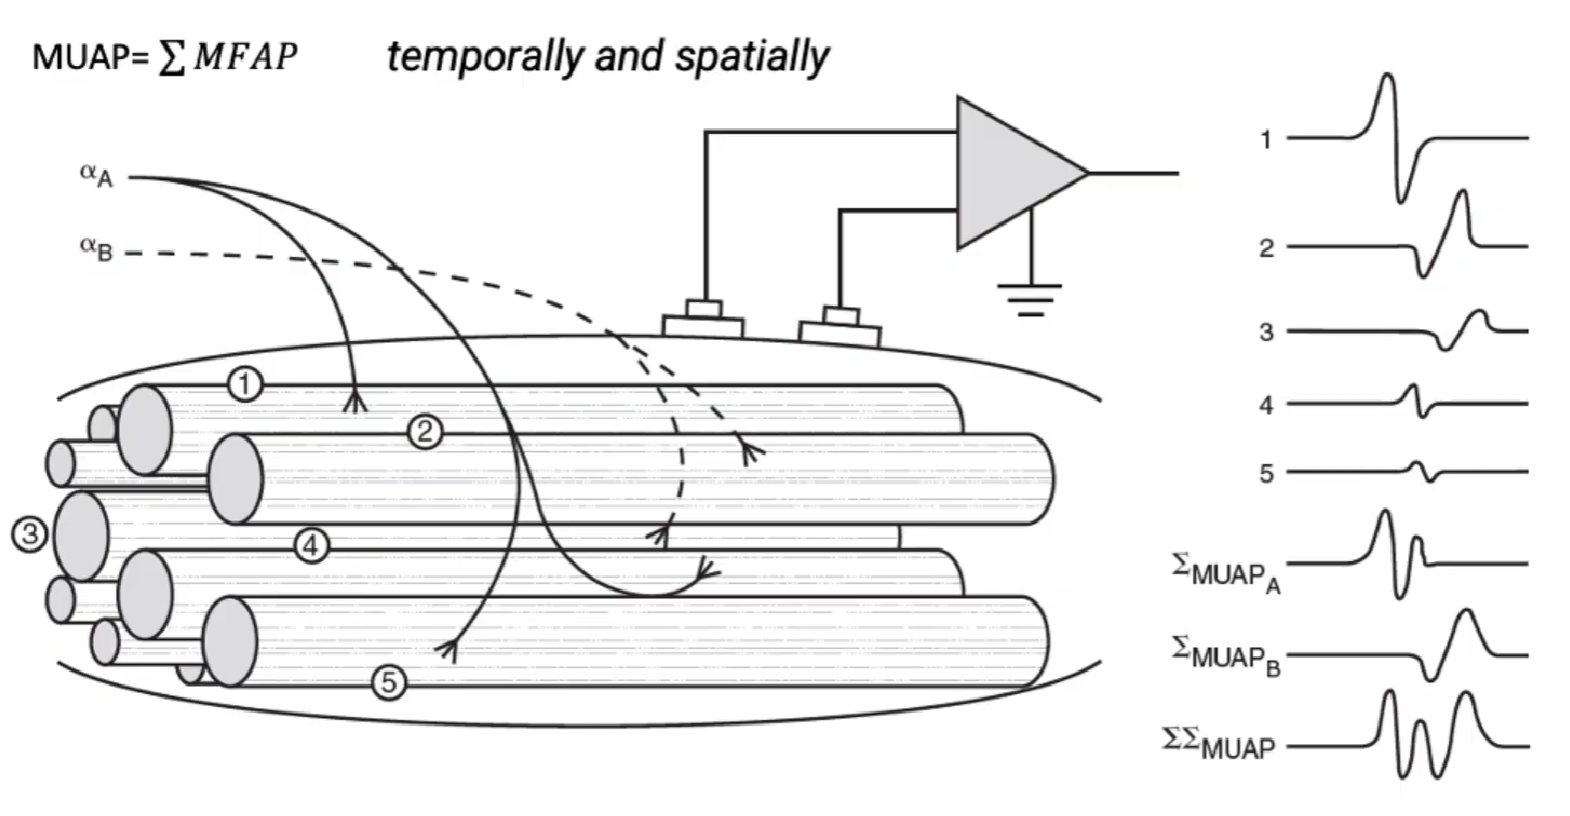
\includegraphics[width=0.55\textwidth]{images/AP_fibres.png}
\end{figure}
Assume fibers 1, 4 and 5 start an action potential, the timing in the picture for the spikes on fiber 1 4 and 5 is the same since they are generated by the same motor neuron, as well the action potential on fiber 2 and 3 discharge togheter. When we look at the electromyogram on the surface, we will observe only the cumulative effect of the fibers that discharge togheter, an external electrode will see only the summation.\bigskip 

If more motor neurons activates near in time, we will observe the summation of the potentials from more motor units, this signal is called \textbf{interferential EMG}.\begin{boxobservation}{}{}
     With non invasive methods we can \textit{only} measure interferential EMGs (summation of many motor units action potentials).
\end{boxobservation}
How do our body modulates the contraction of a muscle? What do the action potential of the neurons look like when we want to exert a stronger or weaker force? We have hundreds of thousends of motor units, one way to modulate the force is to engage more or less units (\textbf{rectruitment}). The other way is to involve the same fibers multiple times a second (\textbf{rate coding}). The higher the rate of discharge, the stronger the force is and shorter the fiber gets. These two phenomena can be modulated separately.\begin{itemize}
     \item \textbf{Rate coding}: The firing rate can range from a minimal of 5/10 impulse per second, to a maximal of 60 impulse per second.Early recruited units may decrease their discharge rate when new units are
recruited (experiencing an increase and then a subsequent decline of their
discharge rate increase)
\end{itemize}
\begin{boxobservation}{}{}
     More motor units and greater rate coding means that EMG amplitude increases.
\end{boxobservation}
\begin{figure}[H]
     \centering
     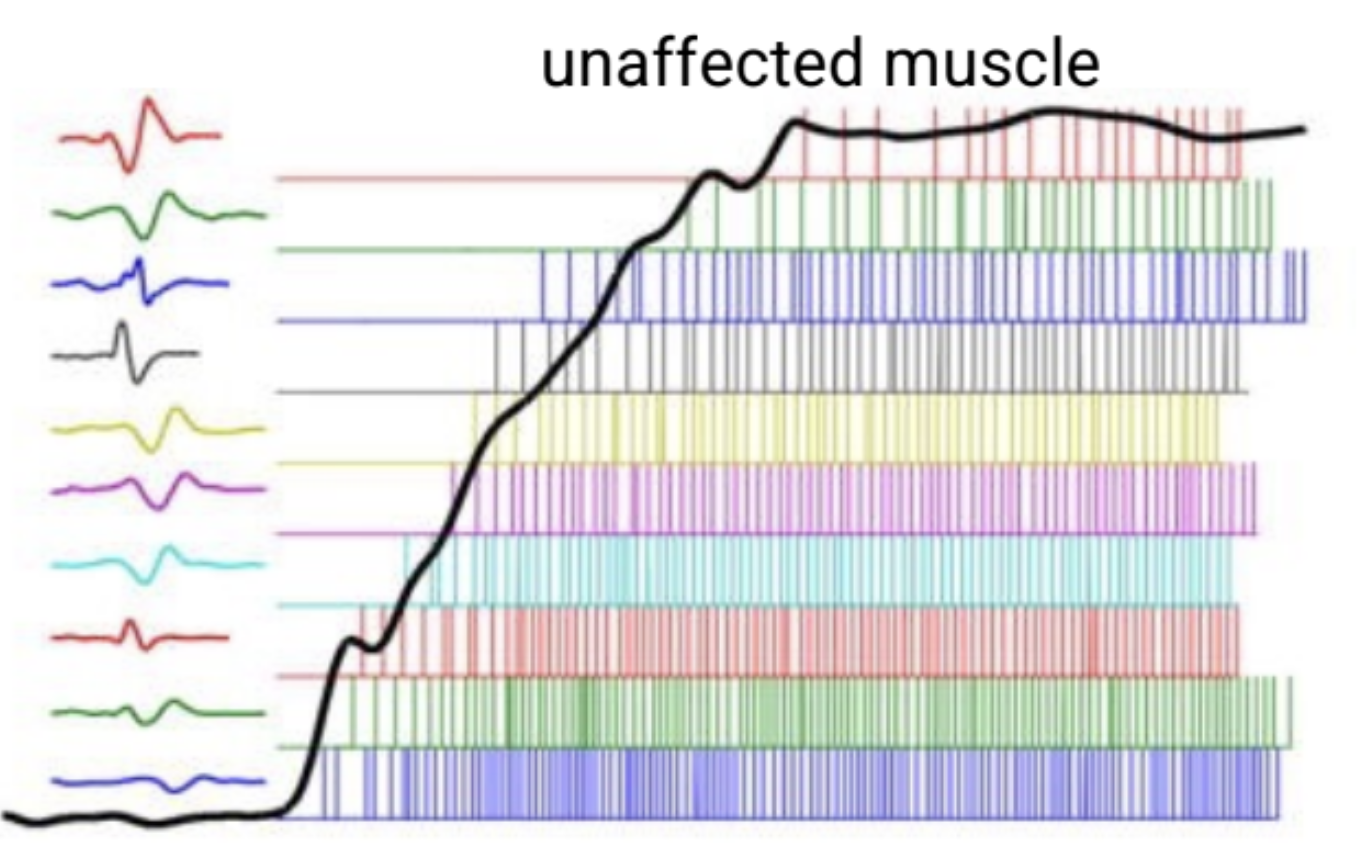
\includegraphics[width=0.4\textwidth]{images/uneffacted_muscles.png}
\end{figure}
\section{Biophysics of the Generation of EMG
Signals}
Non invasive measurment have to deal with signals that passes trough a channel before reaching the sensor, we have  many ways to module the volume condaction of the electrical signals.

Volume conduction properties explain how the size and the shape of the resulting
potential depends on the location on the recording electrode, biological tissues act as spatial and temporal \textit{low-pass}
filters on the potential distribution.
\begin{figure}[H]
     \centering
     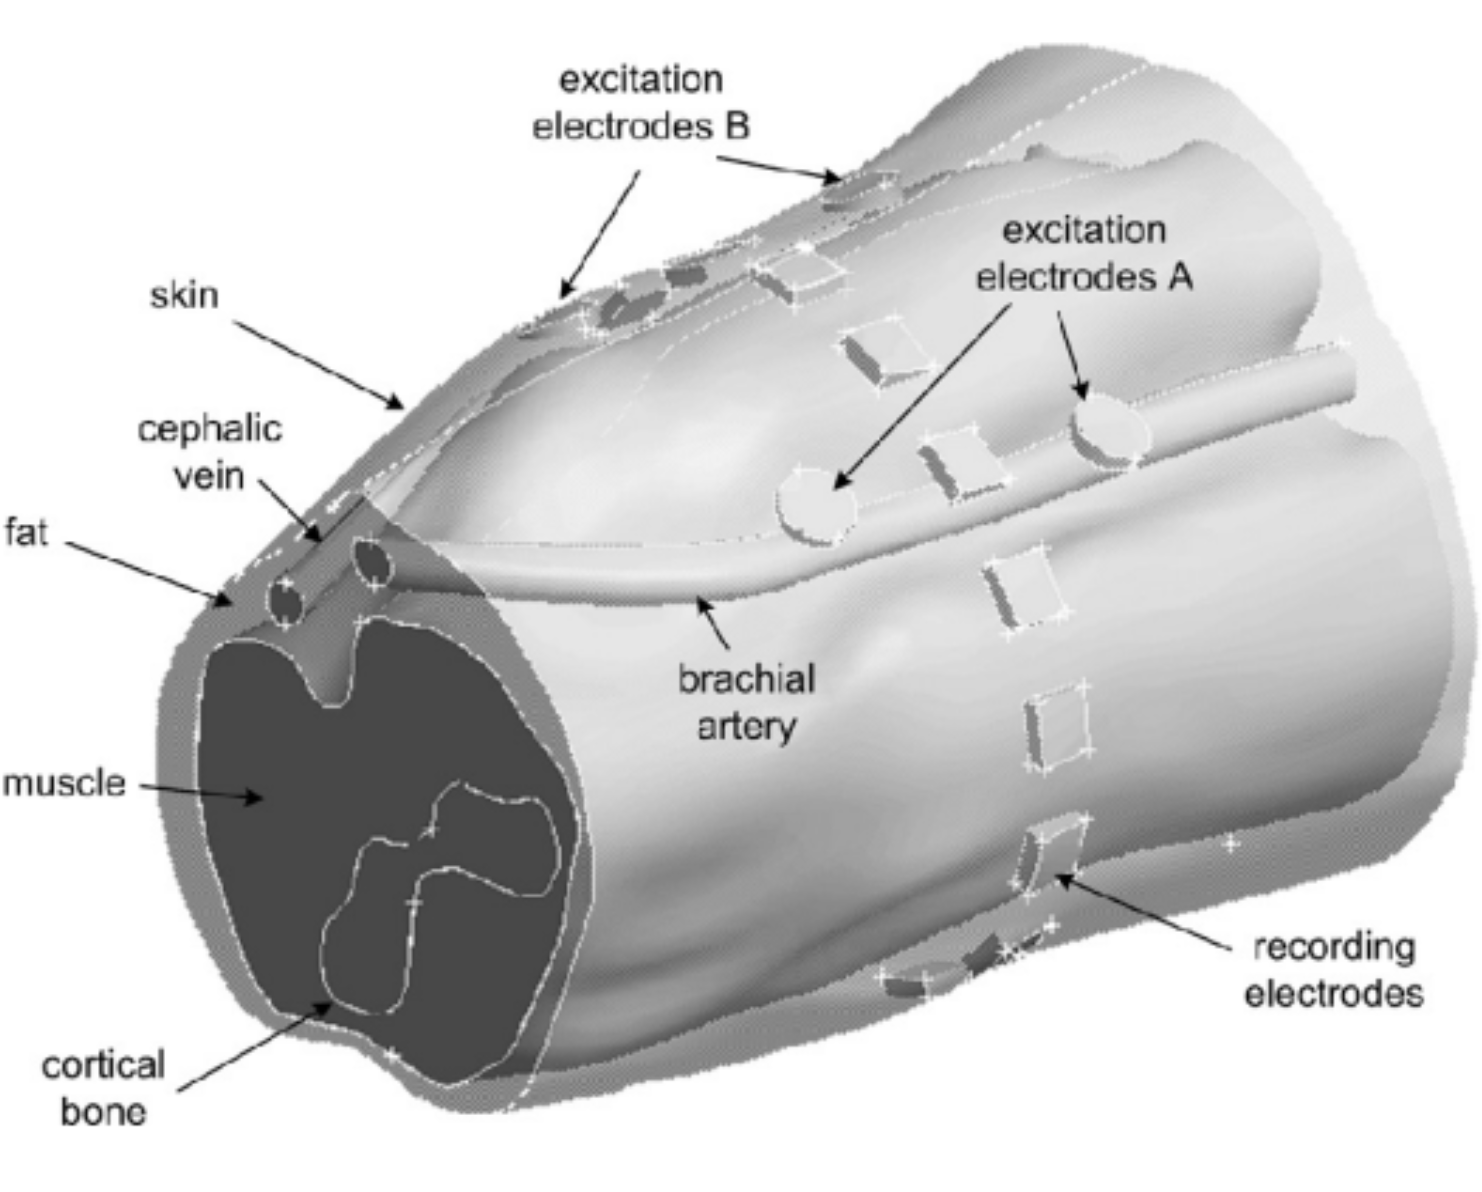
\includegraphics[width=0.35\textwidth]{images/volume_conduction.png}
\end{figure}
One issue is that the sensors are more sensitive to superficial sources than deep sources.
Whichever volume conduction we have (the head for the EEG, the muscle and skin for the EMG) they always behave like a low frequency filter for the conduction of potential. \bigskip

How do we model an action potential? The tripole model consider an action potential as a triple of negative-positive-negative charge that is moving.  
\begin{figure}[H]
     \centering
     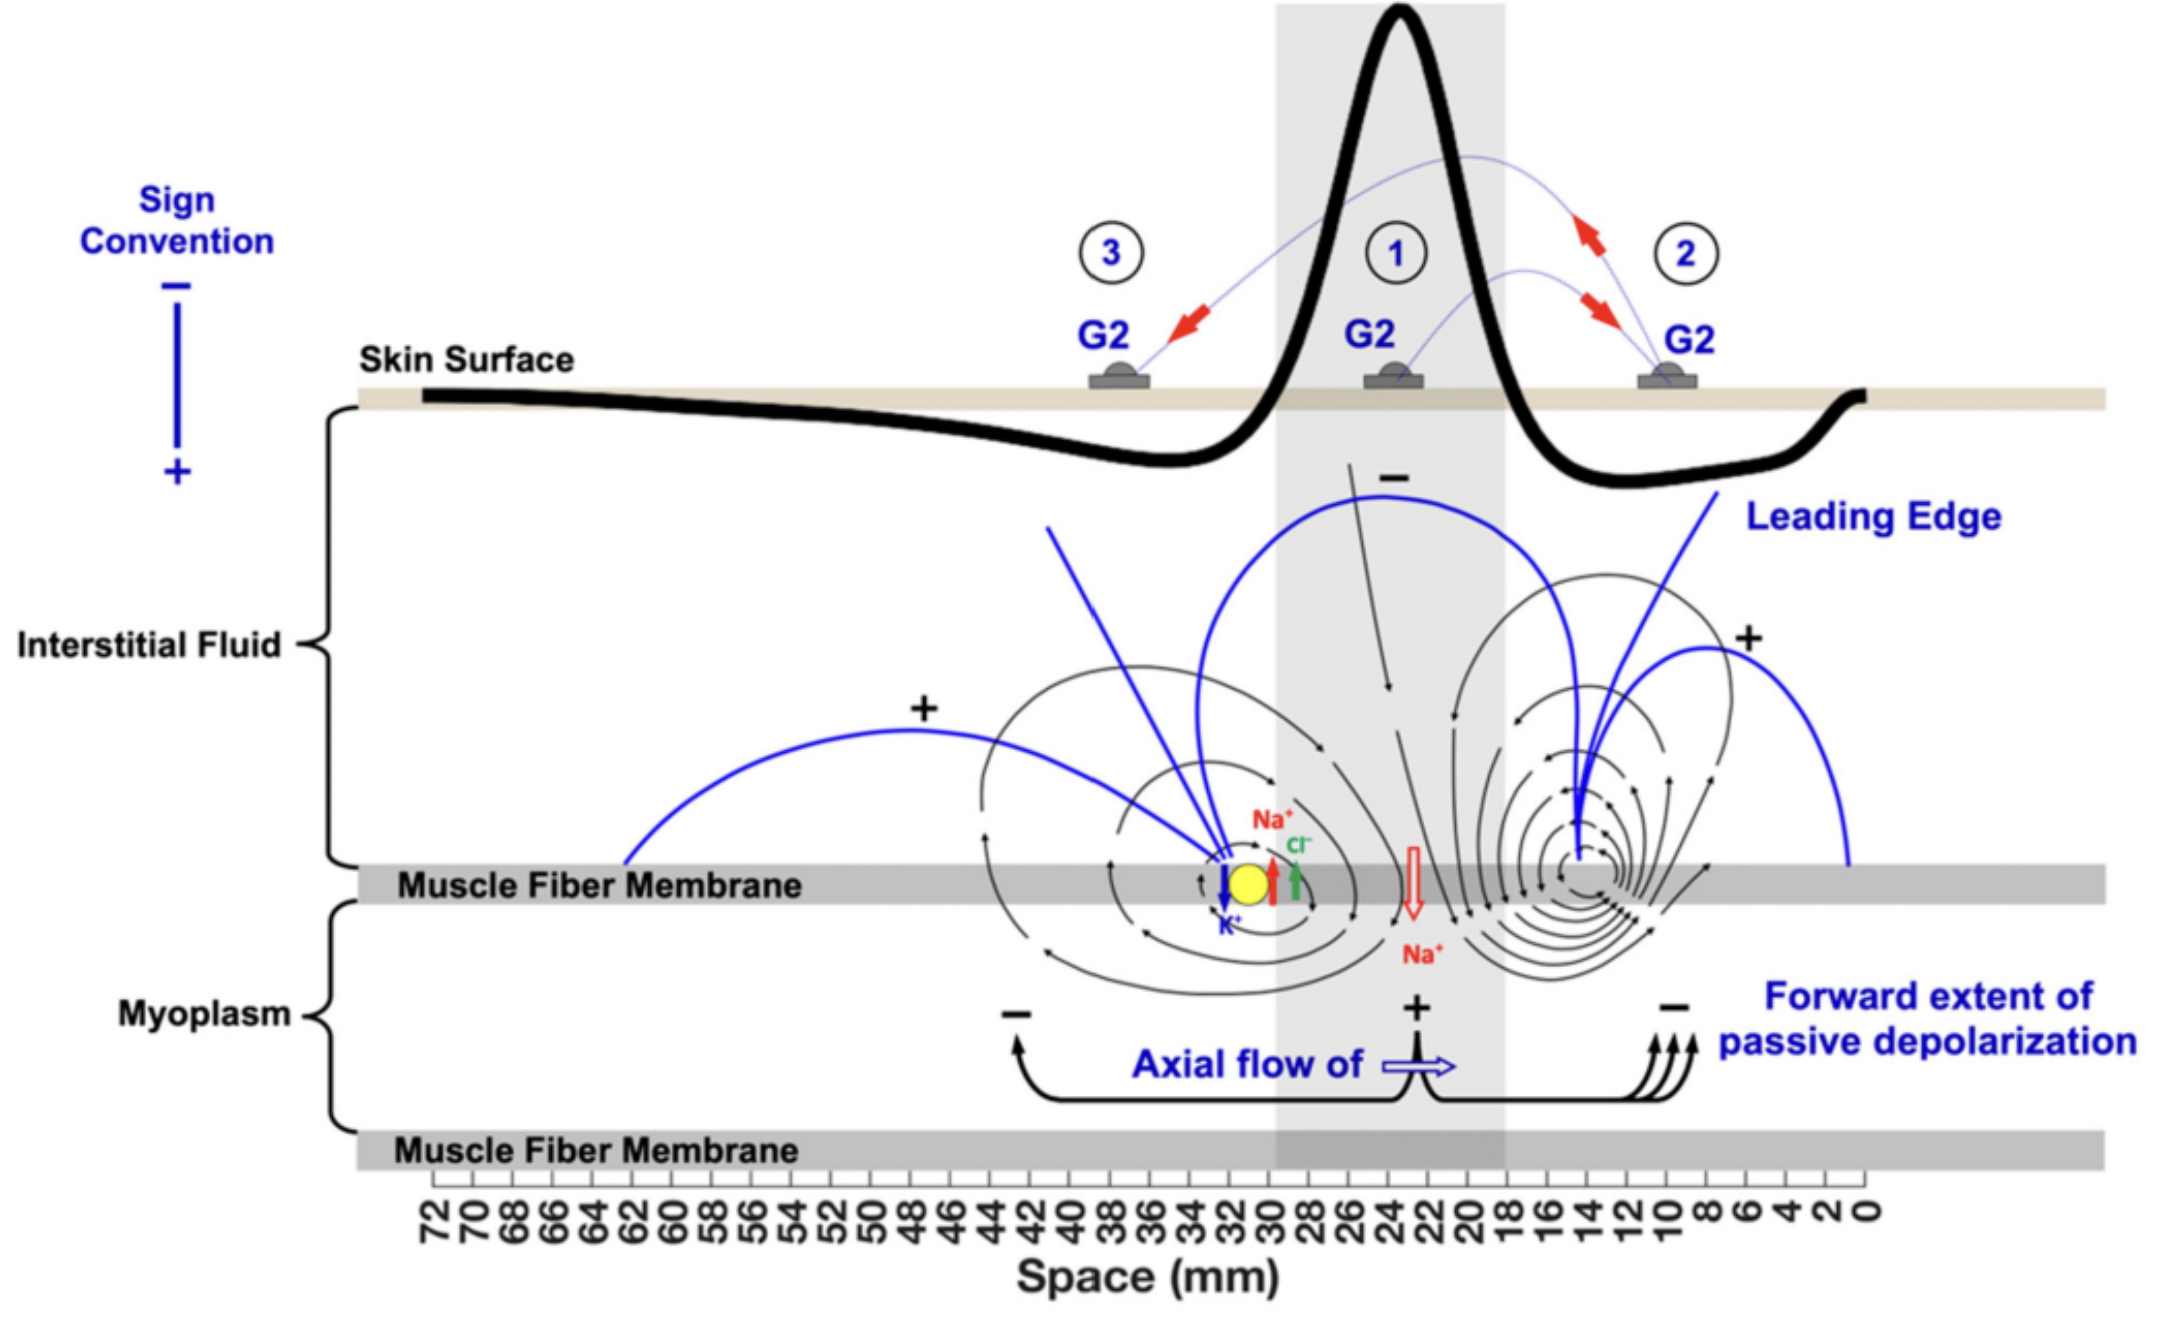
\includegraphics[width=0.6\textwidth]{images/MFAP.png}
\end{figure}
This diagram illustrates the spatial distribution of extracellular potentials and volume conduction during the propagation of a muscle fiber action potential ($AP$) recorded at the skin surface. As the $AP$ travels along the muscle fiber membrane from right to left, it establishes distinct current sources and sinks across the myoplasm and interstitial fluid: a leading edge of passive depolarization ($10{-}14$\,mm), a central zone of active sodium influx and membrane depolarization (shaded gray region, $18{-}30$\,mm), and a trailing region of potassium-mediated repolarization ($32{-}36$\,mm). According to the specified sign convention where upward deflection denotes negativity, a surface electrode ($G_2$) captures a characteristic triphasic waveform at sequential temporal phases (1, 2, and 3) corresponding to the passage of these spatial voltage gradients beneath the recording site.
\begin{figure}[H]
     \centering
     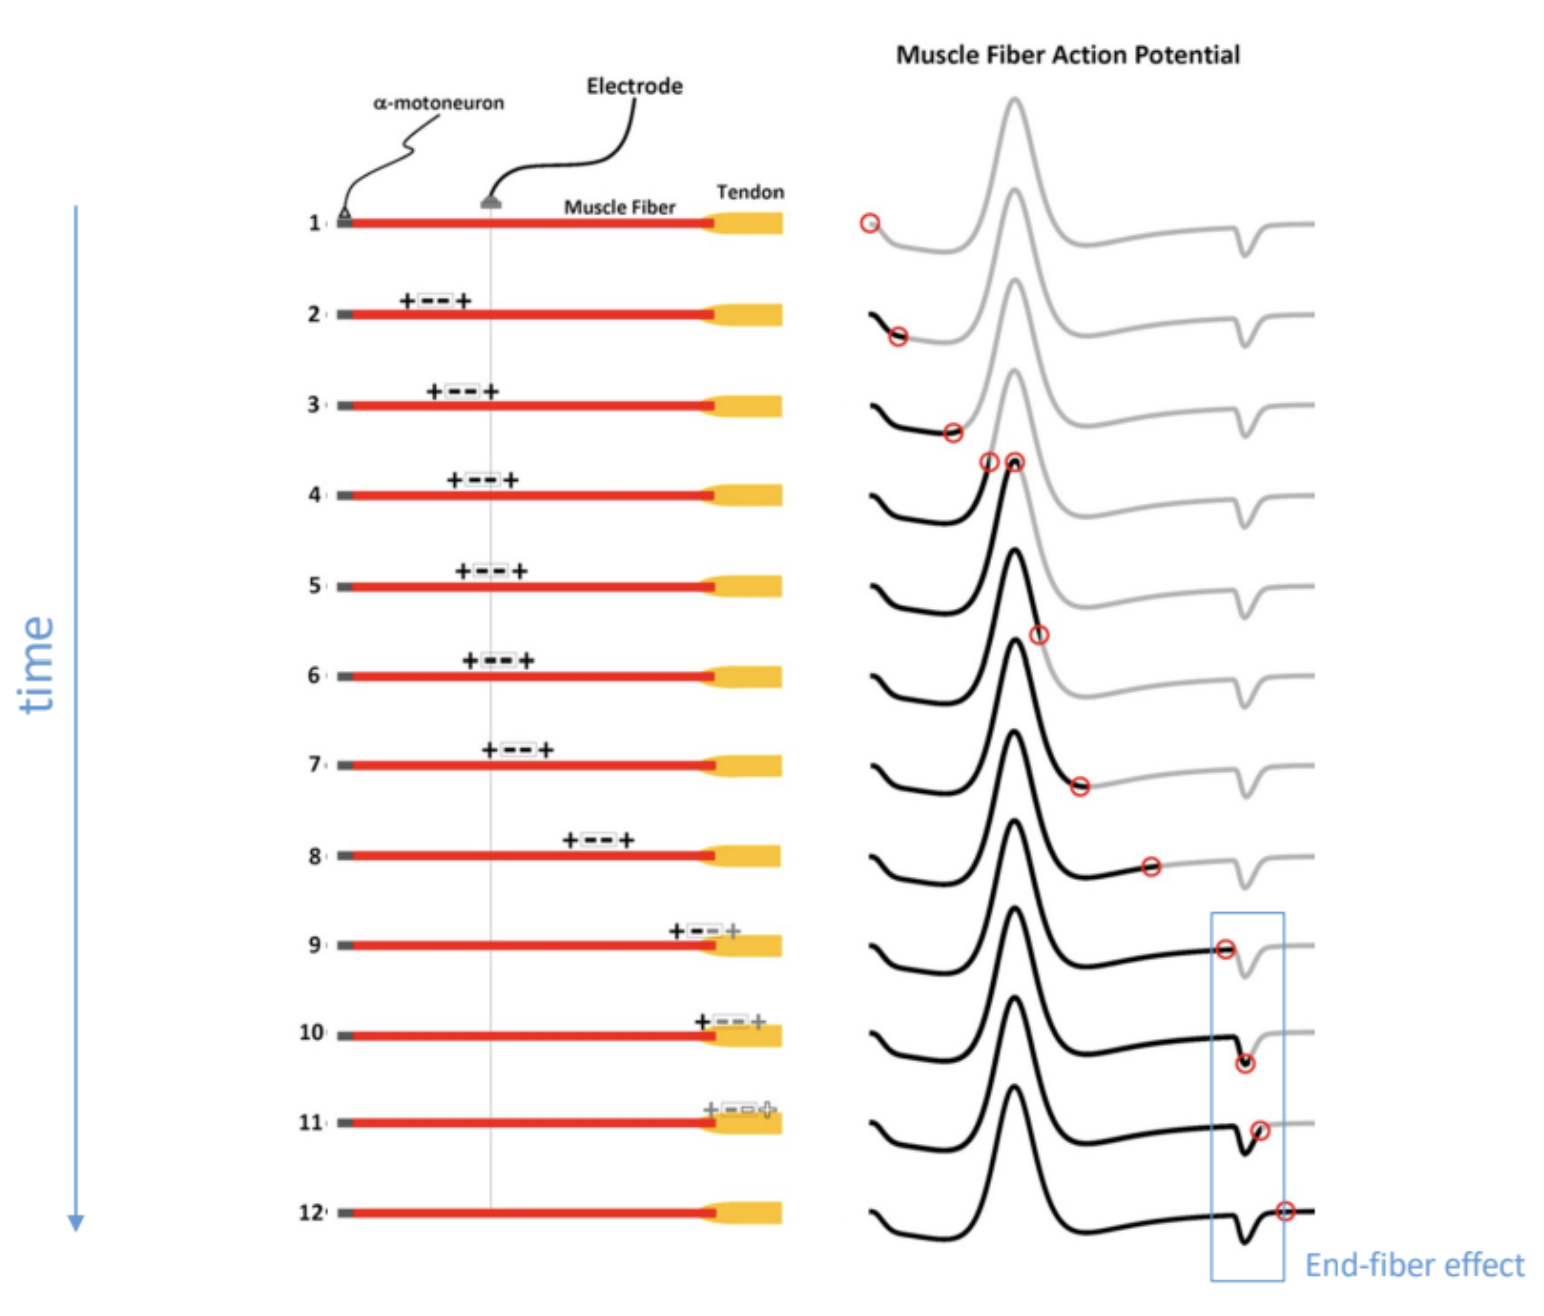
\includegraphics[width=0.4\textwidth]{images/time_dist.png}
\end{figure}
\begin{figure}[H]
     \centering
     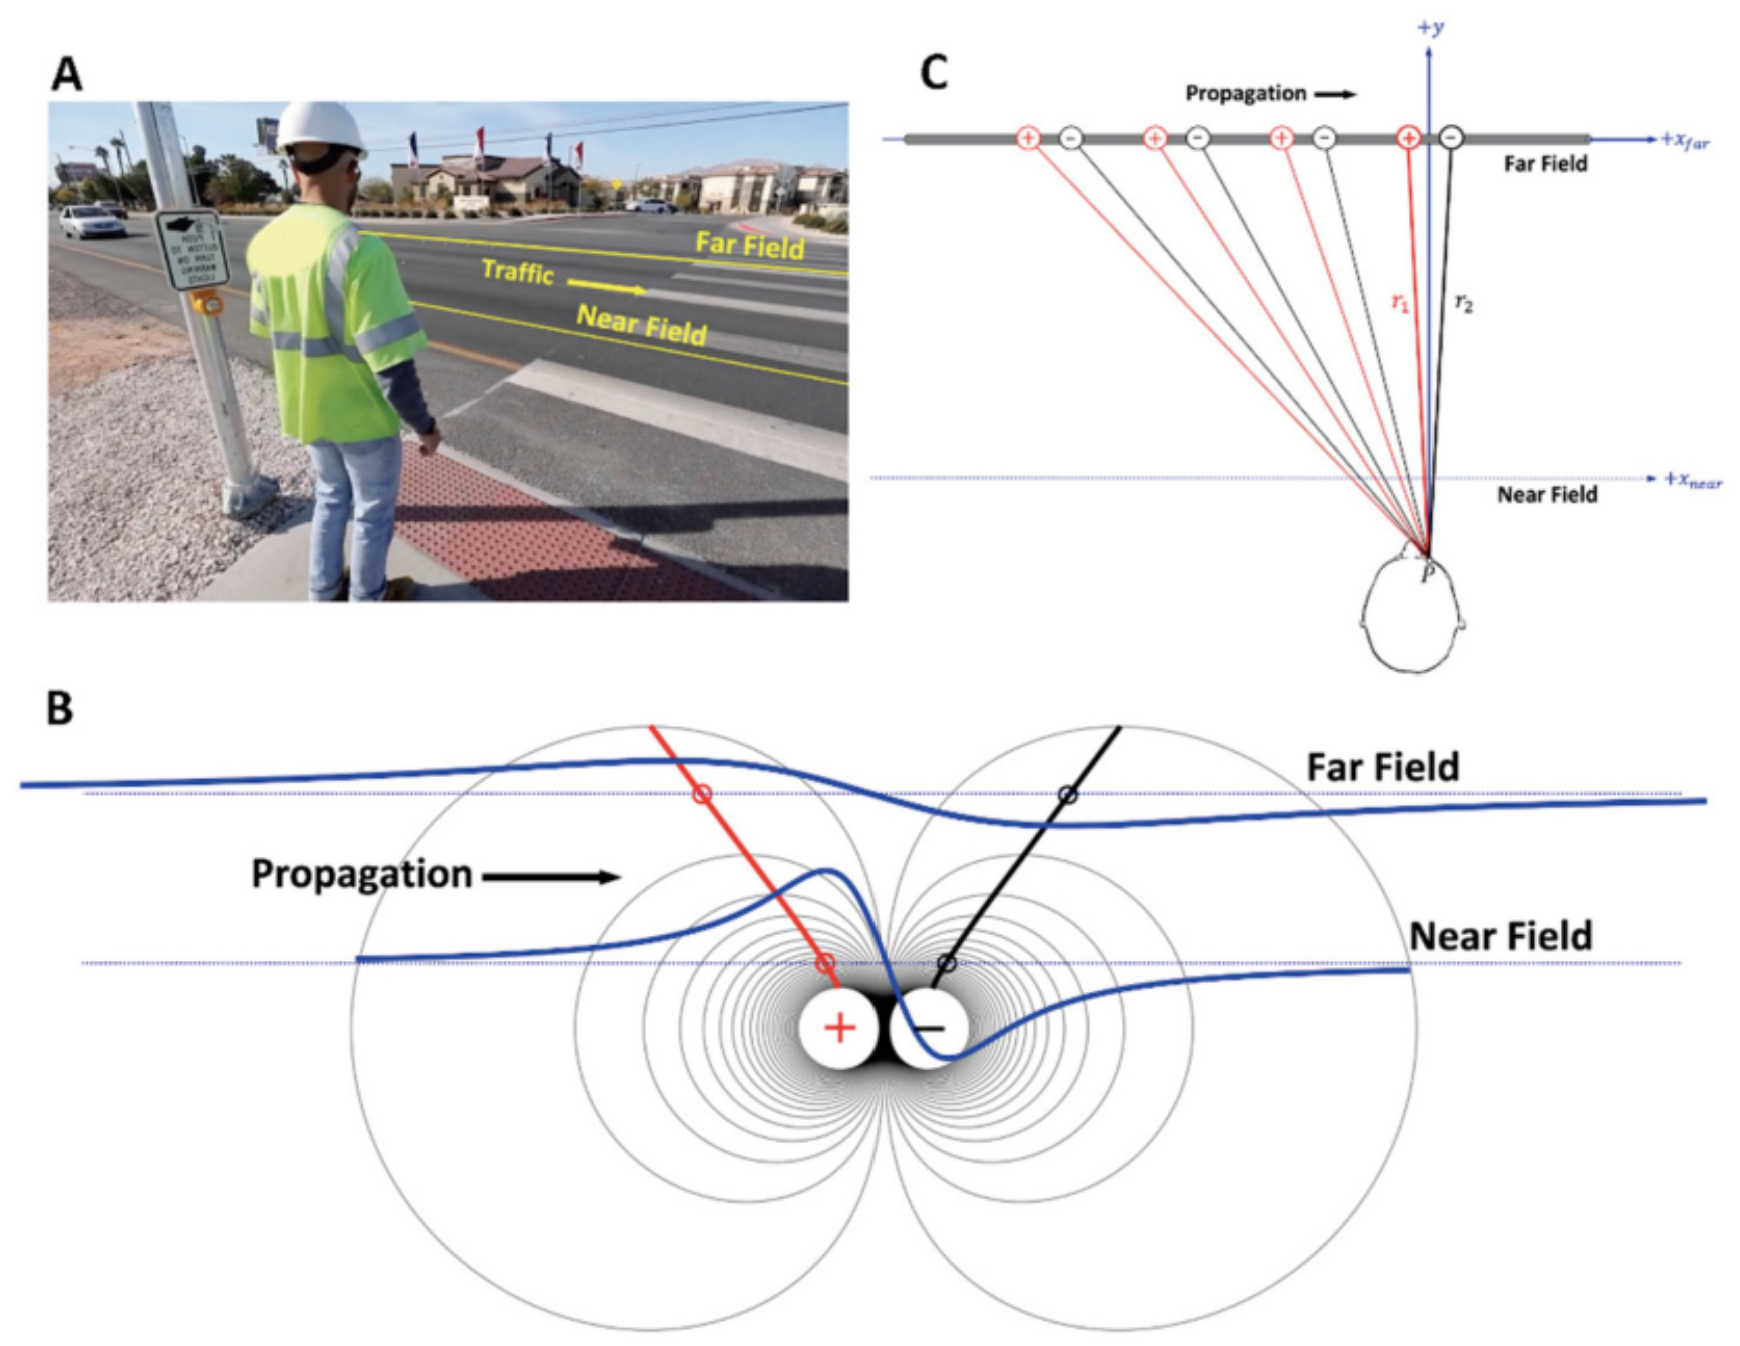
\includegraphics[width=0.4\textwidth]{images/boh.png}
\end{figure}
This image illustrates the differentiation between near-field and far-field detection of Muscle Fiber Action Potentials (MFAPs) in monopolar recordings using a physical analogy and volume conduction geometry.\begin{itemize}\item \textbf{Panel A} presents a real-world traffic analogy: an observer close to the road resolves individual passing vehicles (near-field), whereas a distant observer perceives only a smoothed, collective flow (far-field). \item \textbf{Panel B} depicts the potential fields of the traveling electrical dipole; near-field electrodes capture high-amplitude, high-frequency localized potential changes, while far-field paths yield highly attenuated and spatially blurred waveforms.\item  \textbf{Panel C} formalizes this geometrically, showing that at a large recording distance ($P$), the vectors $r_1$ and $r_2$ to the positive and negative poles become nearly identical in magnitude and angle, causing the opposite electrical fields to largely cancel each other out and result in a low-amplitude, widespread signal.\end{itemize}
\section{Electromyography Instrumentation}
\textit{Adhesive electrodes} can be applied on the skin to register the EMG (can't be used for the EEG due to the hair) anc can be easily stuck on the skin, and doesn't need too much gel. There are also linear array electrods, able to record more spots in a longitudinal way, and 2D array electrodes, able to record a wider surface.
\begin{figure}[H]
     \centering
     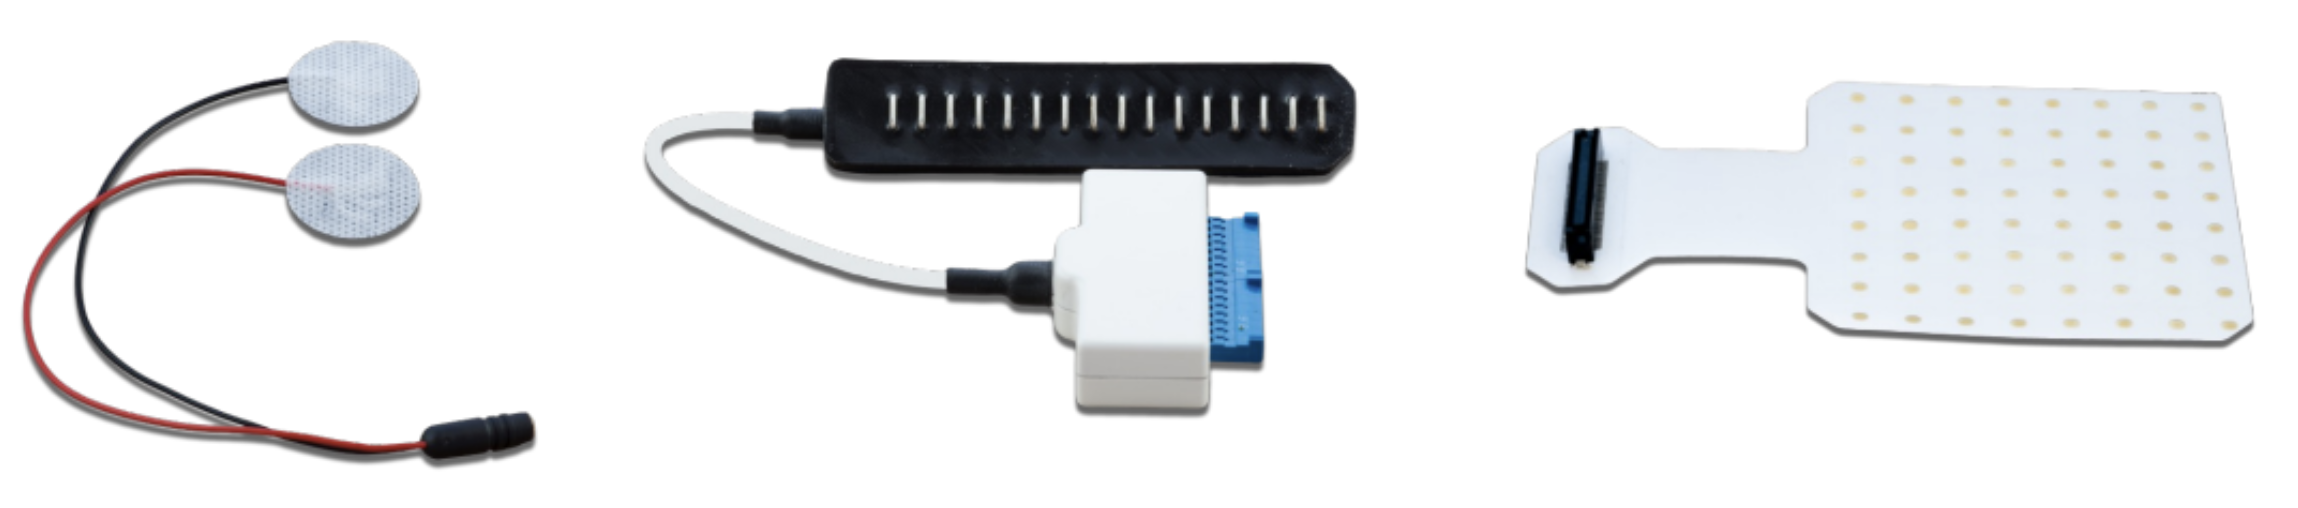
\includegraphics[width=0.6\textwidth]{images/EMG_electrodes.png}
\end{figure}
To measure directly the motor action potential from a single fiber we need to insert a needle inside the muscle, in this case the operator thet performs the EMG must have a deeper knowledge of the human anatomy, since he should know exactly where to place the electrode. 
\begin{figure}[H]
     \centering
     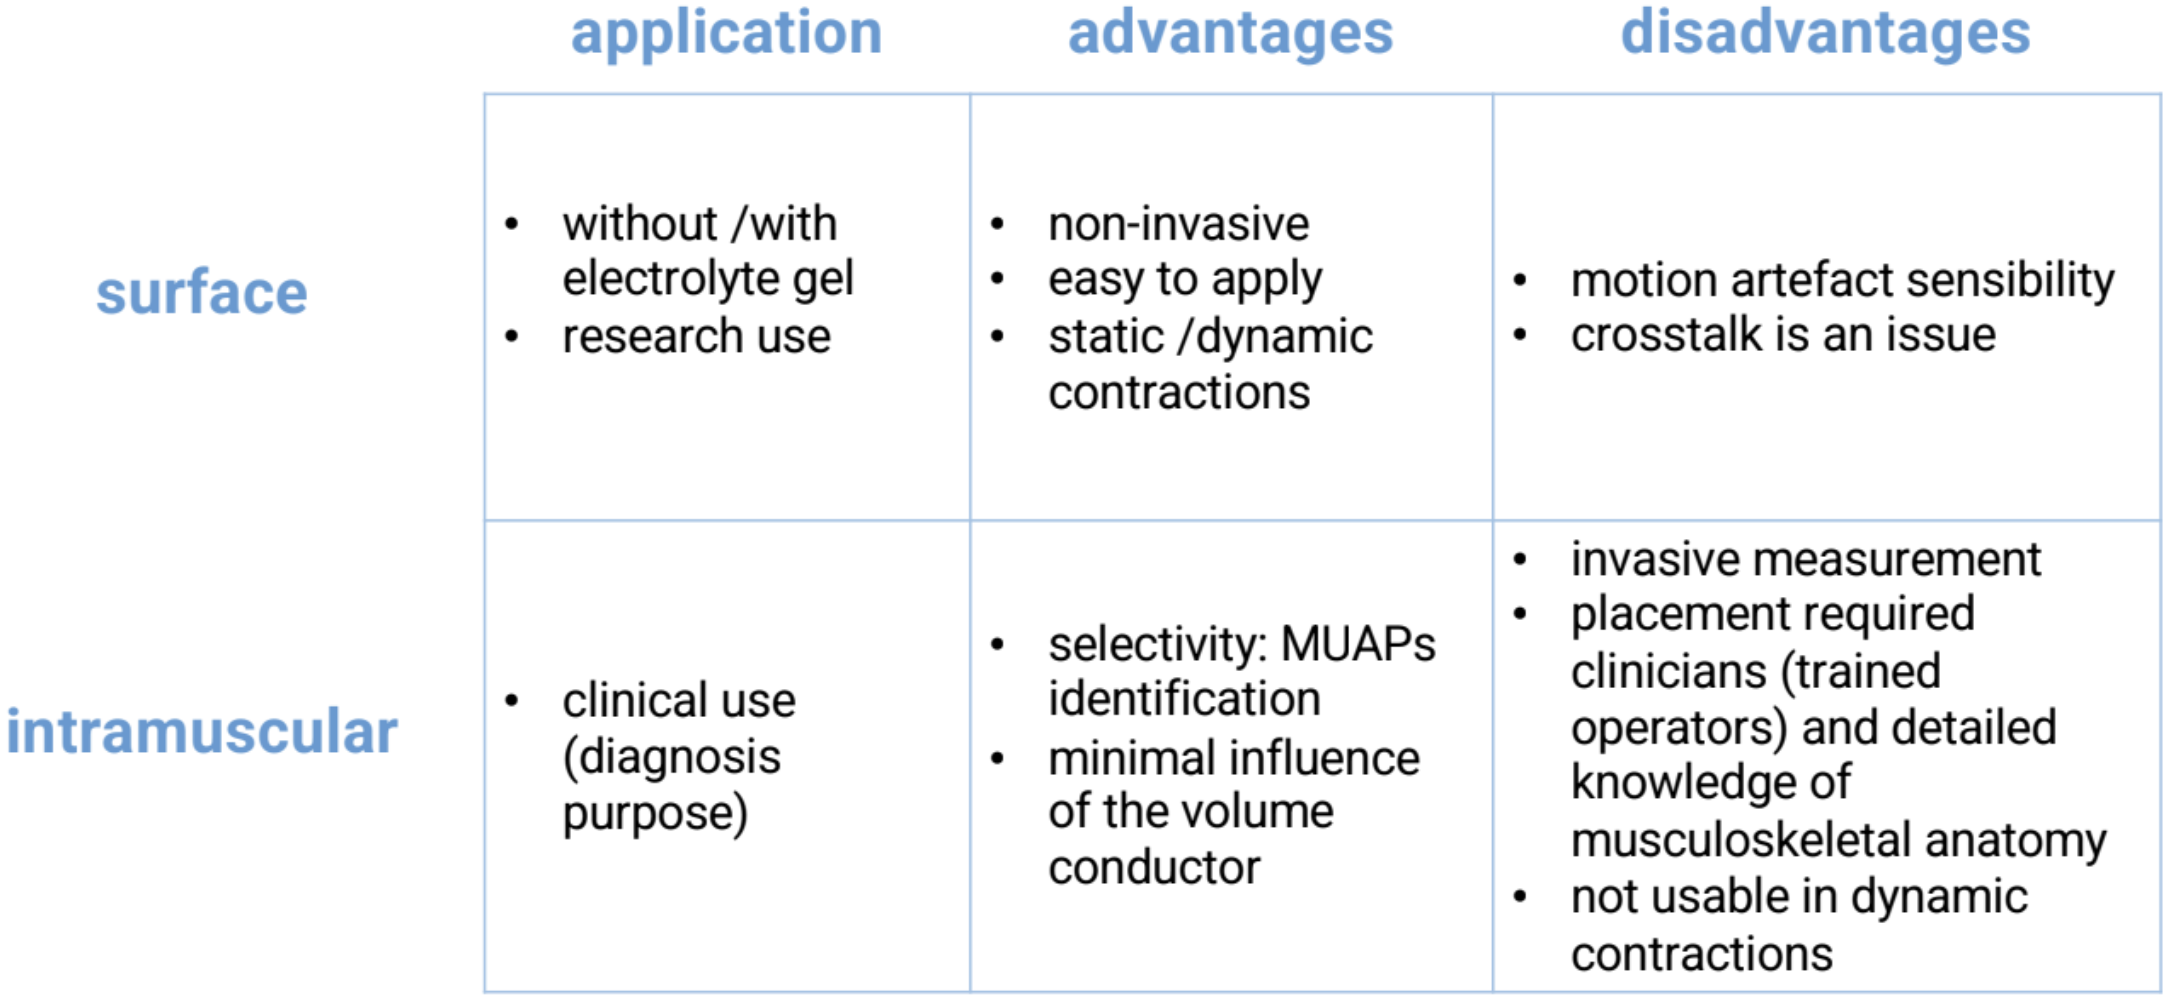
\includegraphics[width=0.6\textwidth]{images/pros_cons.png}
\end{figure}
When you place an electrode, the potential that you record is an average potential field over the area where you place the electrode.
\begin{boxobservation}{}{}
     The larger is the electrode, the lower will be the recorded amplitude, since we are doing an average and we ''miss'' the peaks due to the high frequency components.
\end{boxobservation}
\begin{figure}[H]
     \centering
     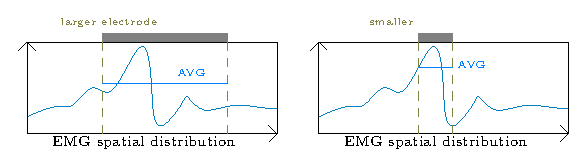
\includegraphics[width=0.7\textwidth]{images/avg_dist.eps}
\end{figure}
The relationship between distribution in time and space of the potential are the same, linked by the conduction velocity of the motor action potential.
\begin{figure}[H]
     \centering
     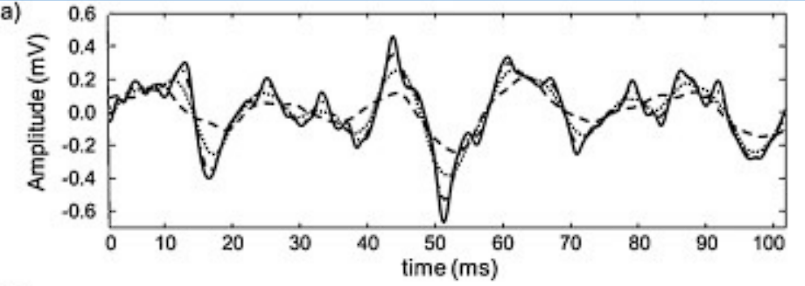
\includegraphics[width=0.6\textwidth]{images/EMG_dist.png}
\end{figure}
This is the time distribution of a recorded EMG, this waveform is similar to the space distribution. The more the electrodes are large, the smoother the recorded waveform will be (due to the averaging).\bigskip

The smoothing is a ''spatial filter'':
\begin{figure}[H]
     \centering
     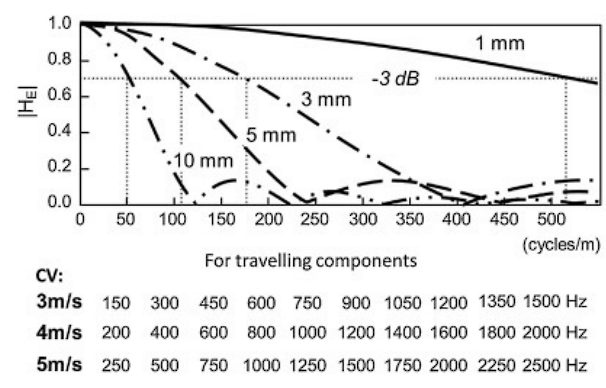
\includegraphics[width=0.4\textwidth]{images/smoothing_filter.png}
     \caption{Section of the transfer function.}
     \label{space_dist}
\end{figure}
The $x$-axis of Figure \ref{space_dist} is expressed in cycles per meter, that is the spatial equivalent of the Heartz, in fact is the representation in the frequency domain of a spatial filter, so instead of Heartz: $\frac{1}{\text{sec}}$ we have $\frac{1}{\text{meter}}$, so the plot is the spectrum of a space distribution. The graph show us different curves relative to different sizes for an electrod, if the electrode is small (1 mm), the filter tends to attenuate less the high frequencies, the larger is the electrode, the stronger is the attenuating effect of the filter.

We consider the cutoff frequency as the usual frequency at which the gain is -3dB. To convert from cycles per meters to Heartz, we need to fix a condutction velocity (as shown in the lower part of Figure \ref{space_dist}).
\section{Electrodes Configuration}
Where do we put the electrodes? For monopolar montage we usually place the reference and ground electrode on bones, and the active electrode on the muscle that we want to measure. For the EMG is more common to use bipolar montage, where we put the ground on a bone and the pair of electrodes on the muscle, usually on the belly (center) of the muscle.
\begin{figure}[H]
     \centering
     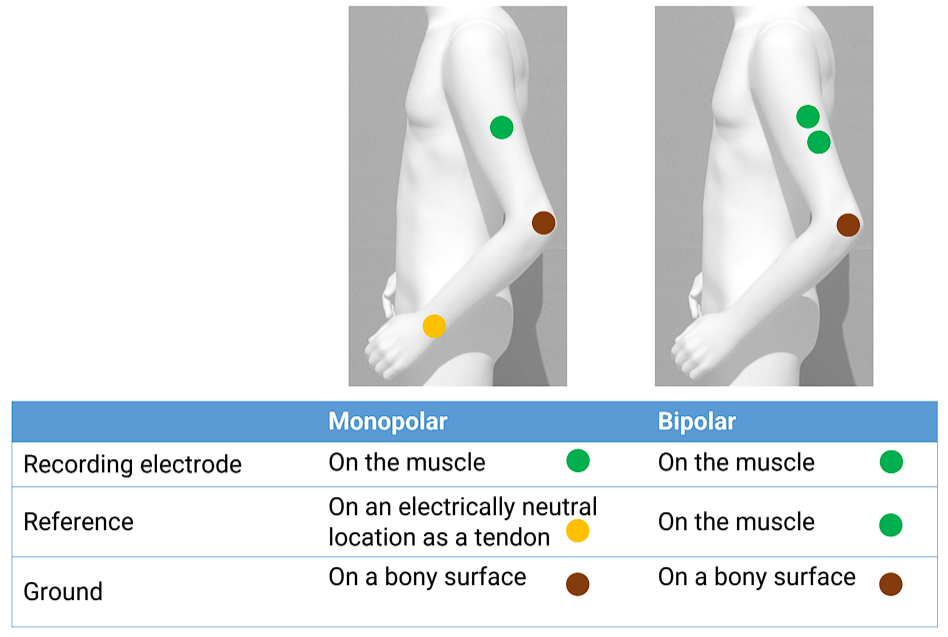
\includegraphics[width=0.5\textwidth]{images/EMG_montage.png}
\end{figure}
Furthermore, the segment between the two electrodes must be parallel to the muscolar fiber. We have to choose properly the \textbf{Inter Electrode Distance (IED)}. We have seen how smaller or larger electrodes affect the recording, now we have to decided how far apart they must be placed: The answer to this question is the following:\begin{boxobservation}{}{}
     The larger is the distance between two electrodes, the lower is the \textit{selectivity}, but the amplitude will be higher.
\end{boxobservation}
\textbf{Selectivity} and \textbf{Detection Volume} are quantities that refers to the same phenomena, observe the following picture:
\begin{figure}[H]
     \centering
     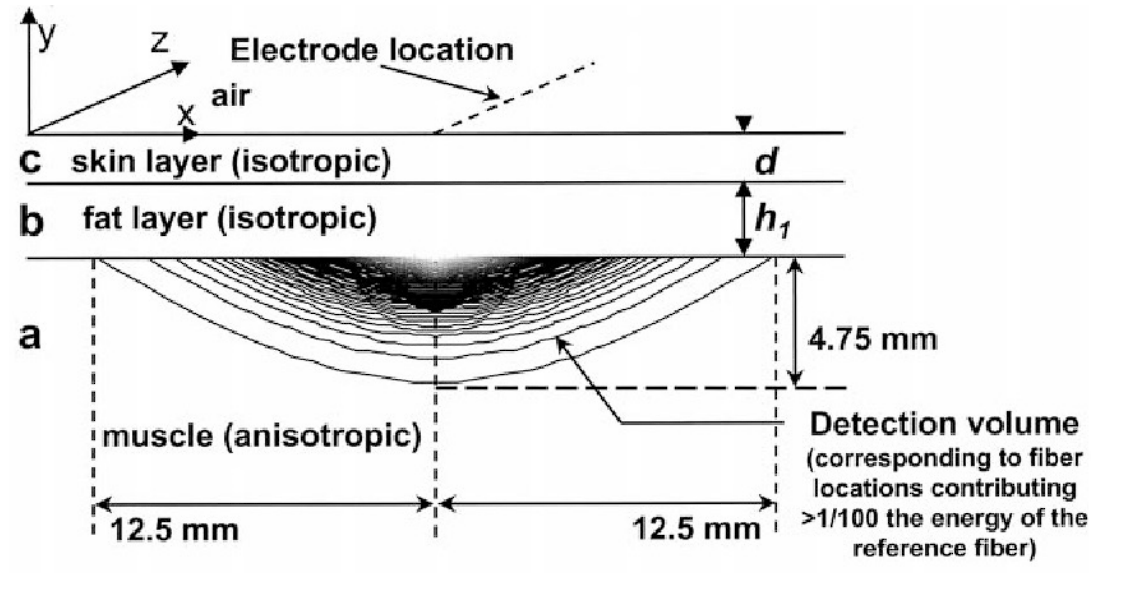
\includegraphics[width=0.5\textwidth]{images/detection_volume.png}
\end{figure}
Is a schematic representation, the negative $y$ axis goes towards the tissue from where we are recording from. The electrical source is in the muscle, we measure the source from the electrode place on the skin. The electrode will record the closest source with maximum amplitude (assuming all the sources have the same strength).

The larger we go from the source, the higher will be the noise with respect to the apparent amplitude. If we take the set of sources for which the apparent amplitude produce an acceptable signal-to-noise ratio, we have the \textit{Detection Volume}.\begin{boxdefinition}{Detection Volume}{}
     The detection volume is the region of the muscle where the sources produce an activity that is detected by the sensors above the noise level.
\end{boxdefinition}
\begin{figure}[H]
     \centering
     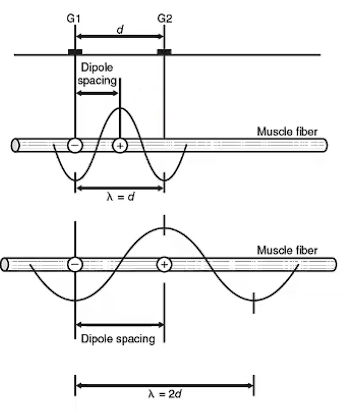
\includegraphics[width=0.3\textwidth]{images/sinewave_in_distr_EMG.png}
     \caption{Two sinusoidal components of the EMG distribution in space.}
     \label{sinewave_in_distr_EMG}
\end{figure}
Consider the 1D spatial distribution of potential on a muscle fiber, this distribution can be expressed (by its Fourier transform) as a superposition of sinewaves. Consider two sinewave components, one of wavelength $d$, and the other of wavelength $2d$:
Let $d$ to be (also) the distance between two electrodes in a pair (the points $G1$ and $G2$ in Figure \ref{sinewave_in_distr_EMG}). We are consider these two electrodes for a bipolar recording. Consider the sinewave whose wavelength is exactly $d$, the potential measured by the amplifier that takes the difference between the potential on $G1$ and $G2$ will be mathematically zero, because $G1$ and $G2$ will be on the same ''part'' of the sinewave.
\begin{boxobservation}{}{}
     Some wave components of the spatial potential distribution will be completely ignored.
\end{boxobservation}
Instead, consider the sinusoidal component of wavelength $2d$. In Figure \ref{sinewave_in_distr_EMG} $G1$ is on the trough and $G2$ on the peak, in this case the difference is the maximum possible.
If the wavelength is $\frac{2}{3}d$, with a trough on $G1$ we would have again a peak on $G2$:
\begin{figure}[H]
     \centering
     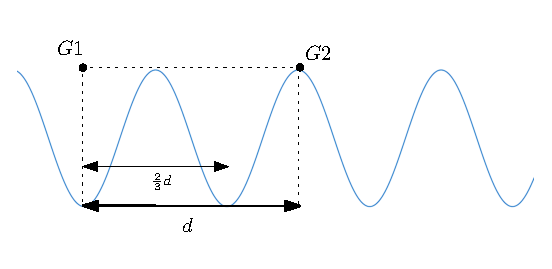
\includegraphics[width=0.6\textwidth]{images/sinewave_in_distr_EMG2.eps}
\end{figure}
Also in this case the difference of potential is the maximum possible. This phenomena in space, is observed also in time: Since the source is moving in the muscle fiber, spatial filtering effects become temporal filtering effects and some frequency components are attenuated more than others. The relationship betweeen the distance and the measured potential shows a filtering effect callded \textbf{comb filter}:\begin{figure}[H]
     \centering
     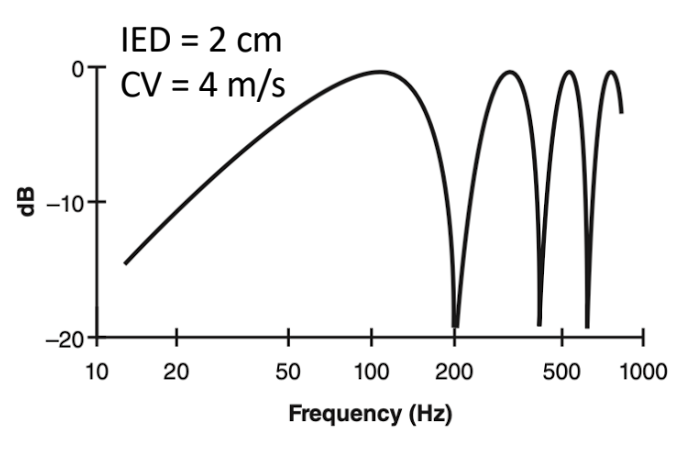
\includegraphics[width=0.4\textwidth]{images/log_freq_DB.png}
\end{figure}
\noindent Observe the following picture:
\begin{figure}[H]
     \centering
     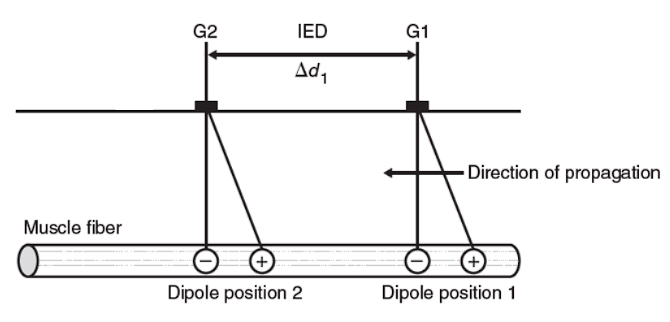
\includegraphics[width=0.6\textwidth]{images/moving_dipole.png}
     \caption{Moving Dipole.}
     \label{moving_dipole}
\end{figure}
A dipole is moving (from left to right) and is represented in two positions (at different times). Consider $\Delta d_1$ as the distance between $G1$ and $G2$. If we measure from $G1$ only, we will record first the negative peak, and then the positive peak (since the negative charge is in front the positive charge in the direction of motion).
\begin{figure}[H]
     \centering
     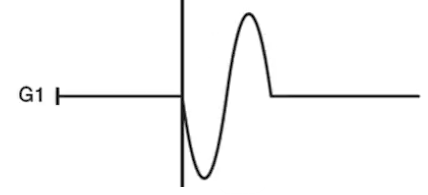
\includegraphics[width=0.3\textwidth]{images/G1_rec.png}
\end{figure}
The negative peak happens when the negative charge is exactly below the electrode $G1$, and the positive peak when the positive charge is there. If we know that $G1$ recorded this potential, we can guess what $G2$ will record,  is exactly the same of $G1$ but delayed until the dipole is under $G2$ (the delay $\Delta t_1$ is given by the distance  $\Delta d_1$  and the condaction velocity).
\begin{figure}[H]
     \centering
     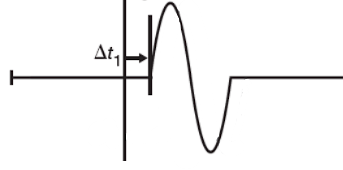
\includegraphics[width=0.3\textwidth]{images/G2_rec.png}
\end{figure}
If we have a bipolar recording we have to take $G1-G2$, we get a ''mexican-hat''-shaped waveform:
\begin{figure}[H]
     \centering
     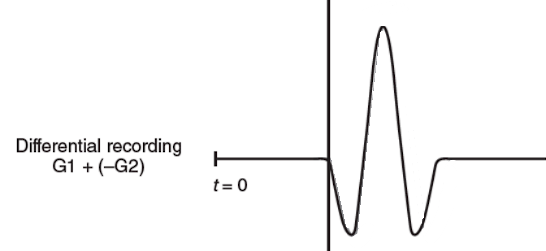
\includegraphics[width=0.4\textwidth]{images/diff_rec.png}
\end{figure}
Let's change the electrodes distace to $\Delta d_2$:
\begin{figure}[H]
     \centering
     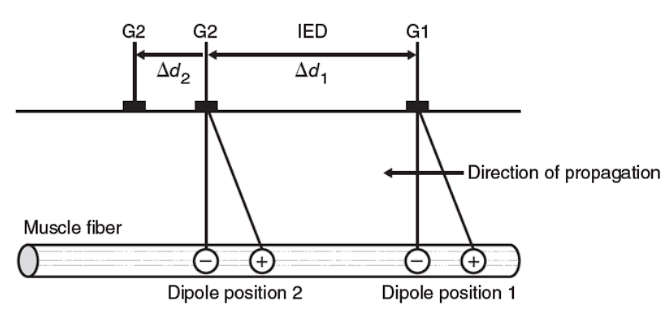
\includegraphics[width=0.5\textwidth]{images/moving_dipole2.png}
\end{figure}
The new delay is denoted $\Delta t_2$, there will be more delay, the gray line in the recording of $G2$ and $G1-G2$ represents this new case where the distance is $\Delta d_2$.  The difference start at the same time but ends later.
\begin{figure}[H]
     \centering
     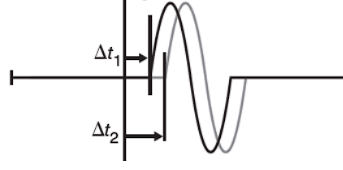
\includegraphics[width=0.3\textwidth]{images/G2_rec2.png}
     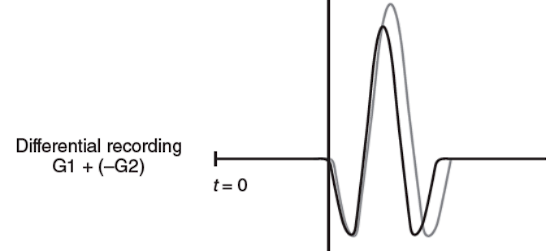
\includegraphics[width=0.3\textwidth]{images/diff_rec2.png}
\end{figure}
\begin{boxobservation}{}{}
     As the
interelectrode distance increases, the time that it takes for the muscle fiber action potential to travel
from $G1$ to $G2$ increases. The resulting differential recording $G1-G2$ is a
muscle fiber action potential that is longer in duration and greater in amplitude.
\end{boxobservation}
\noindent In order to resume these results:\begin{itemize}
     \item The electrode size introduces
a low-pass filtering effect
that attenuates the high frequency components of
both the spatial and
temporal power spectrum of
the spatial EMG.
     \item The (center-to-center) inter electrode distance
introduces a band-pass filtering effect that combines
with the low-pass effect due
to the electrode size to give
the overall filtering effect
depicted in the figure.
\end{itemize}\begin{figure}[H]
     \centering
     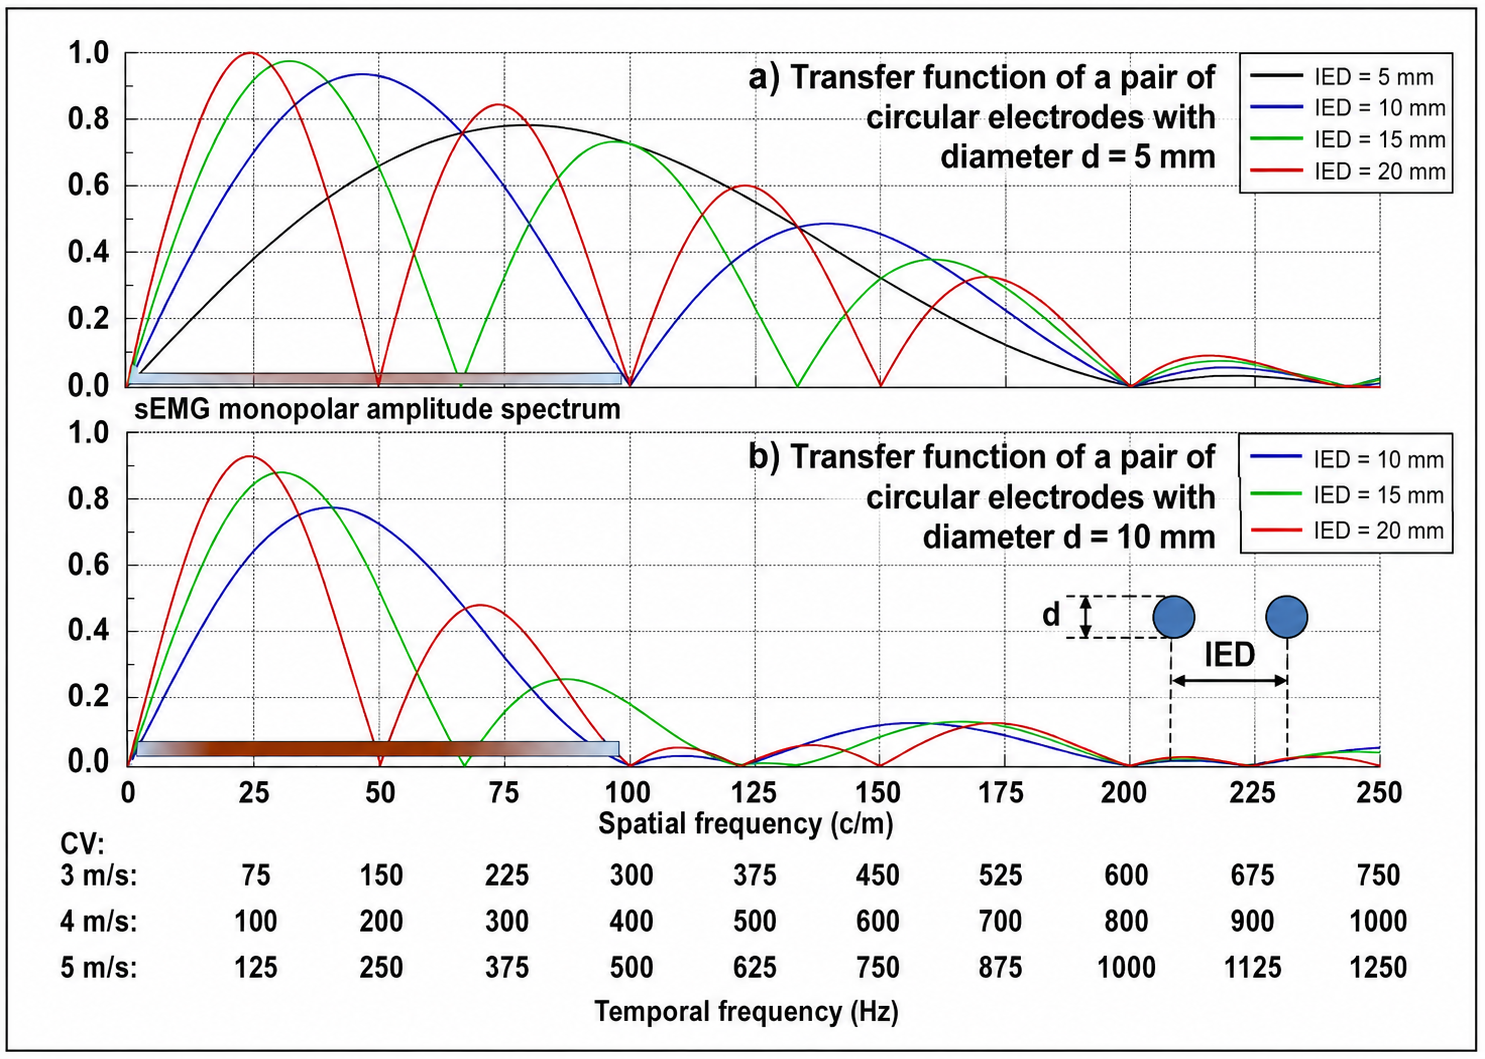
\includegraphics[width=0.7\textwidth]{images/EMG_filtering.png}
\end{figure}
In this image we can see how the main energy components are in the band $[0,100]$ Hz, we can observe how a inter electrode distance (IED) of 20mm place a zero crossing value exactly in the middle of this band, so we should avoid large IED. For IED=10mm, we have 0 gain at 0 and 100 Hz, and the maximum gain at 50 Hz (the middle of the band), we are actually introducing a band-pass filter. With IED=5mm the gain is zero at 0 Hz and higher near 100 Hz, in this case the filter introduced is an high-pass.
\begin{boxobservation}{}{}
     Larger electrode size behaves as stronger low pass filter. The inter electrode distance acts as a comb filter.
\end{boxobservation}
\subsection{Cross-Talk}
Crosstalk refers to the signal that is detected over a certain muscle, but is generated
by another, mostly nearby muscle. It is:\begin{itemize}
     \item Present exclusively in surface recordings when the distance of the detection points
from the sources is of the same order of magnitude for the sources in different
muscles.
     \item Due to the volume conduction properties in combination with the source properties,
and it is one of the most important sources of error in interpreting surface EMG
signals.
\end{itemize}
\begin{figure}[H]
     \centering
     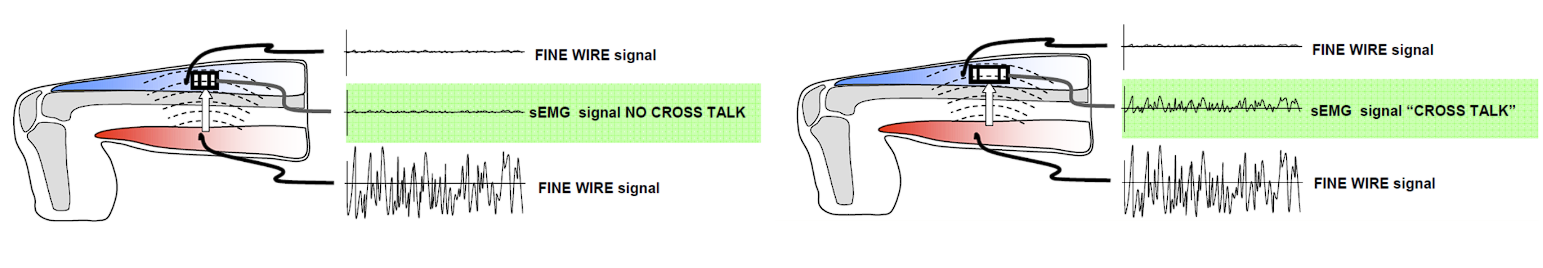
\includegraphics[width=\textwidth]{images/crosstalk.png}
\end{figure}
In real cases there are always some cross-talk.
\subsection{Parameters Influencing the EMG}
EMG signal features depend on anatomical, physical, and detection system parameters. The most important of these factors are:\begin{itemize}
     \item The \textbf{thickness} of the subcutaneous tissue layer (relevant only for surface recordings), if the layer of fat and skin is thicker, the signal amplitude decreases and the signal bandwidth is reduced (spatial and temporal low-pass filter).
     \item The \textbf{depth} of the sources, a deeper source will produce a lower amplitude.
     \item The \textbf{tilt} of the bipolar detection system with respect to the muscle fiber orientation (mainly for surface recordings).
     \item The \textbf{length} of the fibers, shorter fibers have relatively large end-of-fiber potentials. 
     \item The location between \textbf{innervation zone and tendon} (for bipolar derivations).
     \item The \textbf{spatial filter} (electrode montage) used for signal detection, including the electrode size and inter electrode distance.
     \item The \textbf{crosstalk} among nearby muscles (for surface recordings)
\end{itemize}
\subsection{Biosignal Amplifier}
Biosignal amplifiers are essential for recording electromyographic activity, where maximal isometric contractions can yield surface electromyography (sEMG) amplitudes up to $5\,\text{mV}$ and intramuscular EMG amplitudes up to $10\,\text{mV}$ due to reduced tissue attenuation. Critical amplifier specifications include differential gain—which suppresses common-mode noise like power line interference while amplifying the biological signal—input impedance, common-mode rejection ratio (CMRR), and the frequency response relative to the target signals. For hardware conditioning, sEMG activity is typically band-pass filtered between $10\,\text{Hz}$ and $500\,\text{Hz}$; a high-pass cutoff frequency eliminates low-frequency motion artifacts from cables and electrodes, while a low-pass cutoff frequency minimizes high-frequency environmental noise. Finally, selecting a proper sampling rate is imperative to avoid aliasing and preserve signal integrity.
\begin{figure}[H]
     \centering
     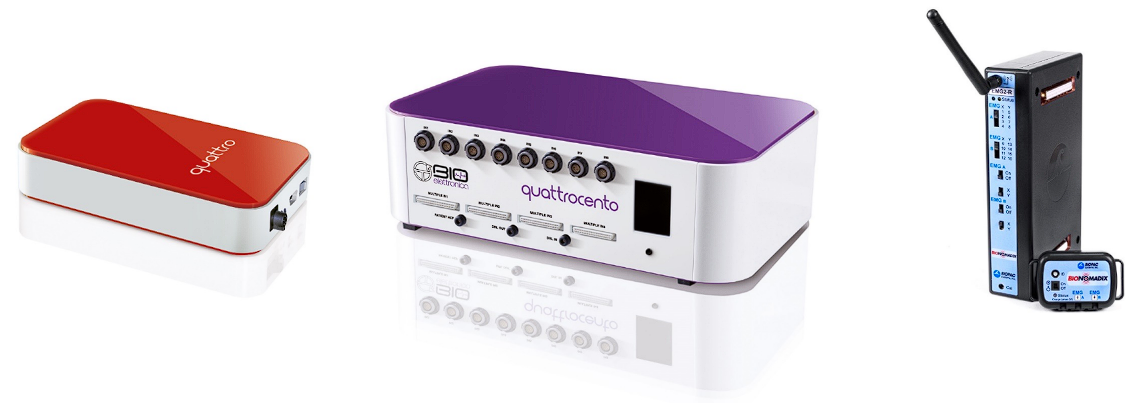
\includegraphics[width=0.7\textwidth]{images/biosignalAmplifier.png}
\end{figure}
\begin{boxobservation}{}{}
     The EEG is usually below 30-70 Hz, the EMG is usually 250 Hz. The single fiber EMG can get up to 1 kHz.
     The spontaneus EEG has an amplitude of a few tens of \underline{micro}Volts, while the EMG it is in units of \underline{milli}Volts (at least 100 times higher). The \textbf{band and the amplitude} of the EMG is \textbf{quite different} with respect to the EEG.
\end{boxobservation}
\section{EMG Signal Processing}
Processing the signal means to apply algorithms to extract parameters or features to
be used for some purpose such as signal classification or quantification of changes.
We consider single-channel techniques, we consider the potential aquired by one channel, we don't apply procedures that requires multiple channel recordings. Single channel method have advantages and disadvantages:\begin{itemize}
     \item \textbf{Advantages}: applicability to a number of
     experimental conditions and
     recording systems, used in basic and applied studies
     concerning sports, ergonomics and
     prevention of neuromuscular
     disorders.
     \item \textbf{Disadvantages}: no information about Motor Units.
\end{itemize}
The following picture is an overview of what have to be done in order to obtain a clean waveform of an EMG (starting from raw data).
\begin{figure}[H]
     \centering
     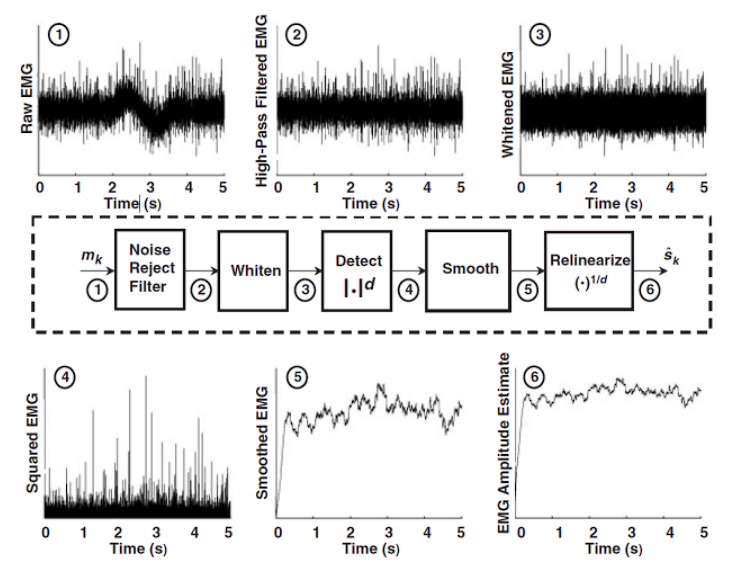
\includegraphics[width=0.7\textwidth]{images/EMG_sig_proc.png}
\end{figure}
The first step is to ''clean'' the data from the noise and artifacts, can be assessed trough:\begin{itemize}
     \item proper skin preparation and
electrode setup,
   \item  analog filtering in the amplifier,
   \item  digital filtering in post-processing.
\end{itemize}
The next step is \textbf{whitening}: make samples statistically
uncorrelated. The correlation between neighbouring
EMG samples is a consequence of the
limited signal bandwidth which reflects
the actual biological generation of EMG
and the low-pass filtering effects of the
tissues. Successive samples of EMG signal are
correlated: the signal correlation
temporally weights the information.\bigskip 

Then there is the \textbf{detection/demodulation} step that consists in taking the absolute value of the signal (can be considered also the squared absolute value). At that step we have a positive signal, now we want to \textbf{smooth} it, i.e. reduce random fluctuations in
the EMG amplitude estimate. We can perform a time averaging with a sliding time window (usually 100-250 ms), or we can apply a linear low pass filter with a cut off frequency between 1 and 6 Hz.

Lower cut off frequencies are appropriate when the
muscle activities under study are constant effort (or
slowly force-varying), and higher cut off frequencies
are appropriate for studies including rapid changes
in muscle effort. \bigskip 

At the end, if the signal was squared during the detection/demodulation phase, we have to take its square root to reconstruct a signal of the correct/original scale.\bigskip

Note that the amplitude of EMG is affected by confounding factors such as the
subcutaneous layer thickness, the inclination of the fibers with respect to the detection
system, the interelectrode distance selected and so on. Normalization can greatly facilitate
comparisons between muscles,
between recording sessions, or
between subjects.
The most frequently employed
normalization procedures is the use
of a \textbf{maximum voluntary contraction
(MVC)}.
\begin{figure}[H]
     \centering
     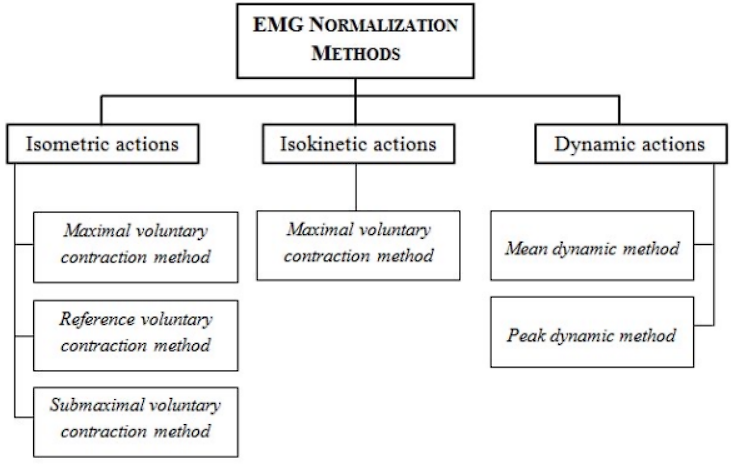
\includegraphics[width=0.5\textwidth]{images/MVC.png}
\end{figure}
the \textbf{double threshold algorithm}, a method used in the processing of electromyographic (EMG) signals to precisely determine the \textbf{onset} of muscle activation.

To decree the start of activation, the signal (in particular the envelope of the EMG signal) must simultaneously satisfy two conditions:\begin{itemize} 
\item Amplitude threshold ($A_c$): The amplitude of the signal envelope must exceed a certain statistical threshold value, denoted as $A_c$. This threshold is usually calculated as a multiple of the RMS (Root Mean Square) value of the signal recorded at rest (when the muscle is relaxed).
\item Temporal threshold ($t_c$): The signal must not only exceed $A_c$, but must remain stably above this threshold for a continuous time interval that is greater than a predefined minimum duration, indicated as $t_c$.
\end{itemize}
\begin{figure}[H]
     \centering
     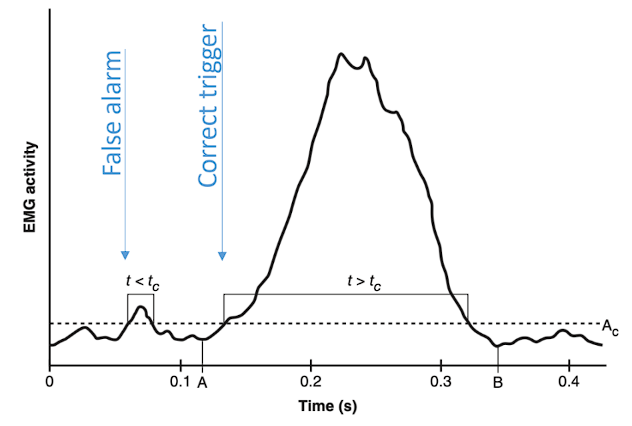
\includegraphics[width=0.5\textwidth]{images/EMGonest.png}
\end{figure}
The \textbf{power spectral density} functions from
different muscle groups all share the same
basic shape, generally related to the shape of
the underlying motor unit action potentials. The main difference between muscle groups
is the bandwidth of the signal, which is related
to the physiology of the muscle.
These properties include:\begin{itemize} 
\item the percent MVC over which motor units are
recruited
\item maximum firing rates
\item muscle fiber lengths.
\end{itemize}
During voluntary contractions the spectral content of the EMG signal progressively
moves towards lower frequencies. This phenomenon can be described as a
compression or frequency scaling of the spectrum; that is, the shape of the spectrum
does not change but only the scale factor of the frequency axis changes.
The median (MDF) and mean (MNF) frequencies are traditional measures of the
frequency content of the signal that require signal stationarity for their use. Let $P(f)$ to be the power spectrum of the EMG:\begin{align}
     &\text{MNF}=\frac{\displaystyle\int_0^{\nicefrac{f_s}{2}}fP(f)df}{\displaystyle\int_0^{\nicefrac{f_s}{2}}P(f)df}\\[1.5ex]
     &\text{MDF}=\frac{1}{2}\displaystyle\int_0^{\nicefrac{f_s}{2}}P(f)df.
\end{align}
\begin{figure}[H]
     \centering
     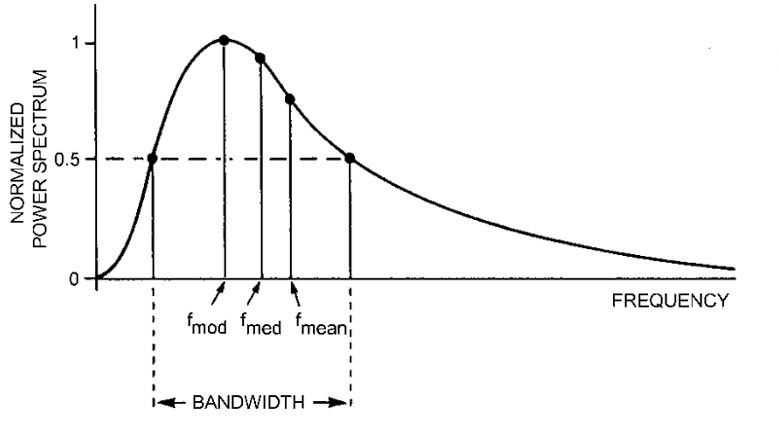
\includegraphics[width=0.5\textwidth]{images/PS_mean.png}
\end{figure}
The MDF and the MNF are single scalar values that tells how the spectral power is compressed towards the low frequencies or the high frequencies.\bigskip 


During a contraction maintained over time, the spectral content of the EMG signal tends to progressively shift towards lower frequencies. The general shape of the spectrum does not change radically, but undergoes ''compression'' or scaling along the frequency axis.

The compression of the frequency spectrum is the direct result of a change in the time domain: the modification of the shape of the MUAP (Motor Unit Action Potential). Due to the mathematical properties of signal analysis, if a wave broadens (becomes slower) in the time domain, its frequency spectrum compresses towards lower values.

What changes the shape of the MUAP? The two main physiological factors responsible for this temporal broadening:
\begin{itemize}
\item Conduction Velocity (CV): A decrease in the conduction velocity of the muscle fibers ''stretches'' the MUAP over time. The duration of the action potential ($\tau$) is inversely proportional to the conduction velocity, governed by the relation $\tau \propto 1/\text{CV}$. Because fatigue slows the propagation of potential along the fiber, the signal takes longer to pass under the sensing electrodes, resulting in a wider wave in the time graph.
\item  pH Change: During contraction, metabolic byproducts accumulate which lower the pH of muscle tissue (making it more acidic). Figure \ref{compression} compare an action potential at normal pH (7.4) with one in an acidic environment (6.6). Acidity alters the dynamics of cell membrane ion channels, slowing the generation of the potential and causing a visible broadening and slight delay of the wave.
\end{itemize}
\begin{figure}[H]
     \centering
     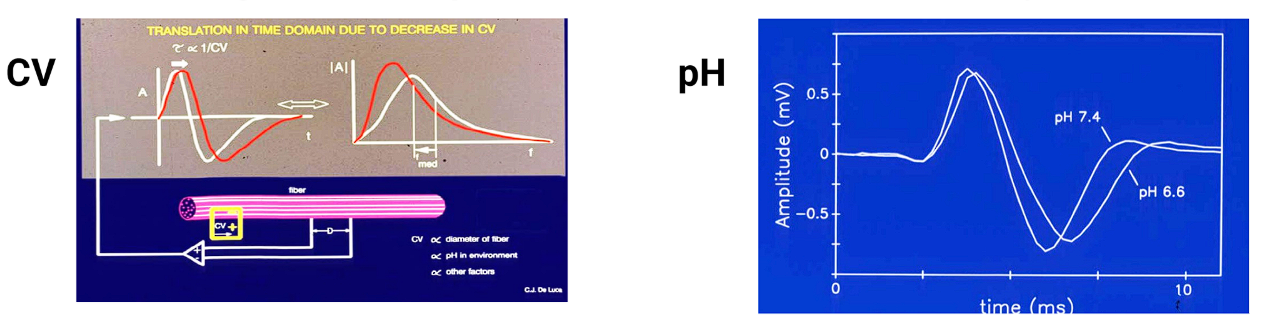
\includegraphics[width=\textwidth]{images/compression.png}
     \caption{Biochemical effect of fatigue.}
     \label{compression}
\end{figure}
\end{document}